\documentclass[12pt, titlepage]{scrartcl}

\usepackage{blubird}
\usepackage[margin=1in]{geometry}
%\usepackage[titletoc,toc,title]{appendix}
%\renewcommand{\hat}{\mathbf}

\usepackage{array}
\usepackage{makecell}
\newtheorem{law}{Law}
\usepackage{float}
\newtheorem{postulate}{Postulate}

\title{Pages in Physics}
\author{Bryan Lu, Rubaiya Emran}
\date{Spring Break 2020}
\begin{document}

\maketitle
\tableofcontents
\newpage

\setcounter{section}{-1}
\section{Introduction}
Well, here we go again. 

One thing's for certain: I have a lot of time on my hands, and everyone does now because of quarantine. At the time of writing, we are all holed up in our homes, responsibly social distancing but also doing not much of anything. 

A couple of years ago, I wrote ``Physics in One Hundred Pages,'' a guide to physics at the AP level, chronicling the basics of mechanics and electromagnetism. Since then, I've learned so much more about other fields of physics and I really wanted to do a continuation of this with all of this extra time. Therefore, this is a new (ongoing) project dedicated to building a repository of physics knowledge at TJ that future years can read quickly, pick up, and distribute. We hope to do this via understandable and accessible entry points, while not ditching a rigorous discussion of the subject. This includes a revamping of the old Hundred Pages, lectures and handouts given at TJ's Physics Team for their A Team during the 2019-2020 school year, and other assorted transcriptions of lectures from classes taught at TJ (most notably from the Quantum/Electrodynamics class during the 2018-2019 school year). 

As one of the principal lecturers of TJ Physics Team's A Team for the past three-quarters of a year, I have formulated some strong opinions on what students should learn in order to round out their physics knowledge, and the contents of this paper reflect that. I also believe that math should be as low as a barrier to entry as possible, so throughout this handout I have chosen to sprinkle in chapters dedicated to relevant mathematics that is used in subsequent chapters. We've arranged the chapters in an order that we think makes sense 

Exercises that I feel are interesting, rewarding, tricky, or otherwise difficult are included, and I've tried to rate the difficulty of each problem from 1-5 stars ($\bigstar$), with more stars implying a harder problem. Obviously, no rating system can be fully objective, but I hope it helps to 
As I am not clever to come up with some of these problems on my own, most have been compiled from a variety of other sources, which will be noted when possible. 

I hope to be clear yet concise, and if anything seems unclear, feel free to contact me through Facebook Messenger, e-mail, or in person. I'm generally willing to help whenever I can.

I have a lot of people to thank for helping me with this project. I'd like to thank Ajit Kadaveru, Jason Chen, Sohom Paul, Jeffery Yu, and Aaditya Singh for helping me through physics when I took the course, editing numerous drafts of the original Hundred Pages, and for help with LaTeX and typesetting everything you see here nicely. A big thank you to the inaugural Quantum/Electrodynamics class under Dr. Osborne's tutelage, in particular Rubaiya Emran (my co-lecturer for this year). Thanks to Dr. John Dell and Dr. Jonathan Osborne, who have taught me a lot of what I know now and have instilled in me a passion for physics. And finally, thanks go out to all of you who read this, who make my work worth something! Your viewing and reading is greatly appreciated. 
\pagebreak

\part{Mechanics}
The first semester is all about the study of mechanics, the study of how physical bodies interact with their environments. An understanding of mechanics is crucial since it serves as the foundation from which the rest of physics is built.  

\section{Building Blocks}
\subsection{Mathematics Excursion I: Calculus}
Before we dive head-first into mechanics, we have to establish our ground rules. Over the course of this handout, we will be using calculus extensively/pretty much everywhere. Some of the prouder physicists would say calculus was invented to deal with mechanics in the first place! In this vein, it's important that we at least have some understanding of what calculus is and how to use it. 

It's okay if this section doesn't make complete sense if you haven't taken a calculus course -- this section is mostly intended to highlight a few important concepts, and as a reference as you proceed through the rest of the handout. You will definitely want to consult other texts to learn and practice calculus more extensively -- TJHSST uses \textit{Early Transcendentals} by Anton, Bivens, and Davis, of which copies can certainly be found online, although we do not condone or encourage the use of piracy to obtain educational materials. 

There are two main parts of single-variable calculus -- differential calculus (dealing with derivatives) and integral calculus (dealing with integrals). We'll look at these two as well as some of the more common applications of calculus to solve problems.
\subsubsection{Derivatives}
Derivatives describe how a function is changing over time. We may as well call it the "slope" of the function - ie. how much a function's output changes with respect to the input. For a function $f$ that is a line, the derivative of the function really is just the slope of the line, because remember that the slope for a line $y = mx+b$ is:
\[
	f'(x) = \dv{f}{x} = \dv{}{x}f(x) = m = \frac{\Delta y}{\Delta x} 
\]	
which is exactly the ratio of the change in the output to the change in the input.\\
The first three expressions are basically equivalent ways to write "the derivative of the function $f$ with respect to $x$." Whatever you want to use is up to you to denote the derivative, but I tend to use different notations depending on the situation. 
\begin{center}
	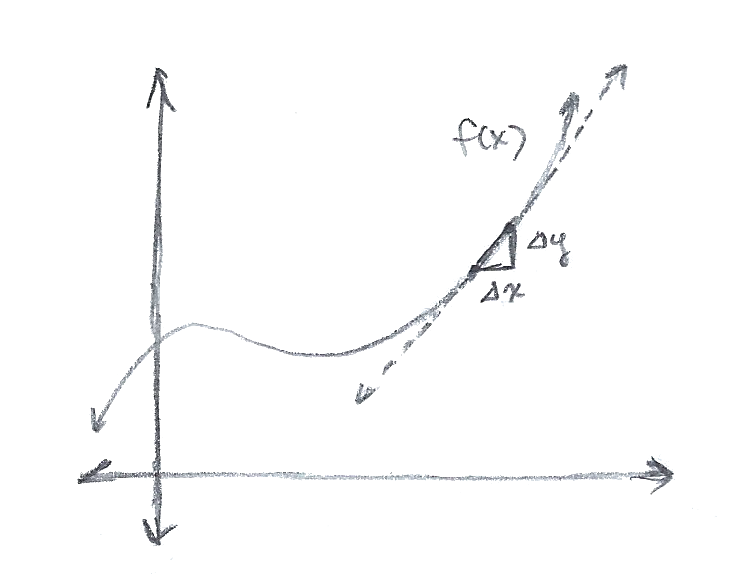
\includegraphics[scale=0.3]{images/math/calc/derivative.png}
\end{center}
What about for non-linear functions? We can still look at how a function's $y$-value changes due to small changes in $x$. If the change in $x$ is small enough, the region of the function around any $x$-value looks kind of like a line anyways. We can find an approximate value for the derivative of a function by looking at the value of the function on the interval $[x, x+h]$, where $h$ is some small real number: 
\[
	\dv{f}{x} \approx \frac{f(x+h) - f(x)}{x+h - x} = \frac{f(x+h) - f(x)}{h}
\]
To get the derivative of $f$, we let the value of $h$ go to zero, to see how the function changes instantaneously. Of course, we can't let $h$ equal zero, because that would be dividing by zero - but we can look at how this expression behaves for values of $h$ close to zero. This is the idea behind taking a limit, which in general allow you to look at what functions do as they approach certain values of $x$ (which you should have learned in TJ Math 5). 
\[
	\dv{f}{x} = \lim_{h\to 0} \frac{f(x+h) - f(x)}{h}
\]
This is the definition of the derivative of $f$ with respect to $x$. With this limit definition, we can start to compute the derivative for more complex functions. Let's look at the derivative of $f(x) = x^2$:
\[
	\dv{f}{x} = \lim_{h\to 0} \frac{f(x+h) - f(x)}{h} =  \lim_{h\to 0} \frac{(x+h)^2 - x^2}{h} =  \lim_{h\to 0} \frac{x^2 + 2xh + h^2 - x^2}{h} = \lim_{h\to 0} \frac{2xh + h^2}{h} = \lim_{h\to 0} 2x+h = 2x
\]
In general, it can be proven that if $f(x) = x^n$, for any real value of $n$: 
\[
	\dv{f}{x} = nx^{n-1}
\]	
This is called the power rule for derivatives. If $n$ is an integer, you can use the binomial theorem - but I'll leave that proof for you to discover. \\
Derivatives also satisfy the following properties, provable from the definition of the derivative:
The derivative of a sum or a multiple of two functions is the same as the sum or a multiple of the derivative of the functions. (This property is called linearity.) 
\[
	\dv{}{x}(f(x) + g(x)) = f'(x) + g'(x) \quad \dv{}{x}(cf(x)) = cf'(x) 
\]
For constant functions $f(x) = c$, we can see that 
\[
	\dv{f}{x} = \dv{}{x} (c) = 0
\]
For the product of functions, we can invoke the product rule, which states that:
\[
	\dv{}{x}(f(x) \cdot g(x)) = f'(x) g(x) + f(x) g'(x)
\]
Closely related is the quotient rule, which is applied for the quotient of two functions:
\[
	\dv{}{x}\left(\frac{f(x)}{g(x)}\right) = \frac{f'(x) g(x) - f(x) g'(x)}{g(x)^2}
\]
Most important of all is the chain rule for the composition of two functions $f(x)$ and $g(x)$:
\[
	\dv{}{x}f(g(x)) = \dv{f}{g} \cdot \dv{g}{x}
\]
What we mean by this notation is that wherever $g(x)$ is substituted in place of $x$ in $f(x)$, we take the derivative of $f(x)$ as if $g(x)$ were the variable, and then multiply by the derivative of $g(x)$ with respect to $x$. It would probably be more clear if I showed you a basic example - Let's look at the derivative of $f(x) = (3x+2)^2$. Let's evaluate this by expanding and taking the derivative of each term:
\[
	\dv{f}{x} = \dv{}{x} (9x^2 + 12x + 4) = 18x + 12
\]
Let's do this using the chain rule, assuming we're looking at the composition of the functions $x^2$ and $3x+2$:
\[
	\dv{f}{x} = 2(3x+2)^{1} \cdot 3 = 18x + 12
\]
The proof of the chain rule is the most complicated, and you can find proofs of all of these facts online. Using the limit definition, we can derive the derivatives of trigonometric, exponential, and logarithmic functions. I've listed them all here in a table:
\begin{center}
	\begin{tabular}{cc|cc|cc}
		\multicolumn{2}{c}{Trigonometric}&\multicolumn{2}{c}{Exponential}&\multicolumn{2}{c}{Inverse Trig}\\ \hline \hline \noalign{\smallskip}
		Function & Derivative & Function & Derivative & Function & Derivative \\ \hline \noalign{\smallskip}
		$\sin x$ & $\cos x$ & $e^x$ & $e^x$ & $\arcsin x$ & $\frac{1}{\sqrt{1-x^2}}$ \\ \hline \noalign{\smallskip}
		$\cos x$ & $-\sin x$ & $\ln x$ & $\frac{1}{x}$ & $\arccos x$ & $-\frac{1}{\sqrt{1-x^2}}$\\ \hline \noalign{\smallskip}
		$\tan x$ & $\sec^2 x$ & $a^x$ & $a^x \ln a$ & $\arctan x$ & $\frac{1}{1+x^2}$\\ \hline \noalign{\smallskip}
		$\cot x$ & $-\csc^2 x$ & $\log_a x$ & $\frac{1}{x \ln a}$ & $\arccot x$ & $-\frac{1}{1+x^2}$ \\ \hline \noalign{\smallskip}
		$\sec x$ & $\sec x \tan x$ & $c^f$ & $c^f \ln c\cdot f'$ & $\arcsec x$ & $\frac{1}{|x|\sqrt{x^2-1}}$ \\ \hline \noalign{\smallskip}
		$\csc x$ & $-\csc x \cot x$ & $f^{g}$ & $f^g \left(f'\frac{g}{f} + g' \ln f \right)$ & $\arccsc x$ & $-\frac{1}{|x|\sqrt{x^2-1}}$ \\ \hline \noalign{\smallskip}
	\end{tabular}
\end{center}
(The function $f(x) = e^x$ is defined so that its derivative is itself. The derivatives of other exponential functions are derived from the chain rule.) Using these principles, we can take the derivative of any elementary function and find out what it's rate of change using these rules.\\
We can also keep taking the derivative of the function as many times as we want, as long as the function is differentiable (meaning that the function is continuous and the limit involved in the derivative exists). We've only looked at the first derivatives of functions so far, but we can always find the second derivatives, third derivatives, etc. of functions. Notation-wise, we use $\dnv{y}{x}{n}$ for the $n$th derivative of a function, or $f^{n}(x)$ where $n$ is either expressed in Roman numerals if $n < 4$ or just written out regularly (which is in my opinion super arbitrary). Usually, however, we rarely go beyond the second derivative in physics. 

\subsubsection{Indefinite Integrals}
Given a function $f(x)$, let's try to find the function $F(x)$ that has $f(x)$ as its derivative. $F(x)$ is called the antiderivative of $f(x)$. We write $F(x)$ as the following:
\[
	F(x) = \int f(x) \, dx 
\]
The $dx$ at the end means that the antiderivative is being found with respect to the variable $x$. The big $\int$ symbol is called an integral, and finding the antiderivative is called taking the indefinite integral (or the integral, for short) - which is what I'll call it from now on, to avoid typing so much. \\
In general, it's much more difficult to integrate functions, and most of the time, the integral of a random composition of functions cannot be expressed as a combination of elementary functions. Let's just look at a simple example to start - the integral of $f(x) = x^2$. We can use a little bit of trial and error to do this. Notice that because of the power rule for derivatives, the exponents in polynomial functions decrease by 1. Therefore, we know that the antiderivative $F(x)$ has to be of the form $F(x) = kx^3$. By definition, 
\[
	\dv{}{x} F(x) = \dv{}{x} \int f(x) \, dx = f(x) 
\]
We know that $\dv{}{x} F(x) = 3 kx^2 = f(x)$. Therefore, $k = \frac{1}{3}$, so at the end of it all, we have:
\[
	F(x) = \int x^2 \, dx  = \frac{1}{3}x^3 + C
\]
Why add the $+C$? Because the derivative of a function eliminates the constant (the derivative of a constant is zero), any constant could have been added to the original function $F(x)$ to produce a derivative of $f(x)$. We can add any constant we want, but if we want to be as general as possible, we use a $+C$ represents any real number.\\
We don't have as many properties that hold in general for the evaluations of all integrals, but at least the properties of linearity still hold. That is, for any two functions, the integral of the sum or constant multiple of these functions is the sum or the constant multiple of the integral of the function:
\[
	\int f(x) + g(x) \, dx = \int f(x) \, dx + \int g(x) \, dx \quad \int cf(x) \, dx = c \int f(x) \, dx
\]
Here's a table of the most common integrals so you can get started: 
\begin{center}
	\begin{tabular}{c c}
		\multicolumn{2}{c}{Most Common Integrals}\\ \hline \noalign{\smallskip}
		Function & Antiderivative \\ \hline \hline \noalign{\smallskip}
		$\int x^n \, dx$ & $\frac{1}{n+1}x^{n+1}$ + C\\ \noalign{\smallskip} \hline \noalign{\smallskip}
		$\int e^x \, dx$ & $e^x + C$ \\ \noalign{\smallskip} \hline \noalign{\smallskip}
		$\int a^x \, dx$ & $\frac{1}{\ln a} a^x + C$ \\ \noalign{\smallskip} \hline \noalign{\smallskip}
		$\int \sin x \, dx$ & $-\cos x + C$ \\ \noalign{\smallskip} \hline \noalign{\smallskip}
		$\int \cos x \, dx$ & $\sin x + C$ \\ \noalign{\smallskip} \hline \noalign{\smallskip}
		$\int \sec^2 x \, dx$ & $\tan x + C$ \\ \noalign{\smallskip} \hline \noalign{\smallskip}
		%$\int \sec x \tan x \, dx$ & $\sec x + C$ \\ \noalign{\smallskip} \hline \noalign{\smallskip}
		$\int \tan x \, dx$ & $\ln |\sec x| + C$ \\ \noalign{\smallskip} \hline \noalign{\smallskip}
		$\int \frac{1}{x}\, dx$ & $\ln |x| + C$ \\ \noalign{\smallskip} \hline \noalign{\smallskip}
		$\int \frac{1}{\sqrt{1-x^2}} \, dx$ & $\arcsin x + C$ \\ \noalign{\smallskip} \hline \noalign{\smallskip}
		$\int \frac{1}{1+x^2}\, dx$ & $\arctan x + C$ \\ \noalign{\smallskip} \hline \noalign{\smallskip}
	\end{tabular}
\end{center}	
We do have some other tricks that we can use to evaluate more complex integrals. The most powerful is called the $u$-substitution, and it changes the variables inside the integral. Essentially, it's like the reverse of the chain rule, and works for integration. Let's just look at an example -  the integral $\int xe^{x^2} \, dx$. At first, this may seem really hard to do - after all, we don't know a function that has this as a derivative from the table, but what we can do is substitute $u = x^2$. When we do this, however, we also have to substitute in a new variable of integration (also called a differential) $du = 2x \, dx$. This is computed by taking the derivative of the substituted expression - note that $\dv{u}{x} = 2x$, so we just "multiply through" by $dx$. We substitute in $\frac{1}{2} u = x\, dx$ so we get:
\[
	\int xe^{x^2} \, dx = \int \frac{1}{2} e^u \, du = \frac{1}{2} e^u + C
\]
We can't leave our answer in terms of $u$, so we substitute back in to get: 
\[
	\int xe^{x^2} \, dx = \frac{1}{2}e^{x^2} + C
\]
Selecting the proper $u$-substitution for an integral can make the difference between making your job difficult and making your job easy. It takes a lot of practice to find the right $u$-substitution to simplify the integral to one of the most common integrals. \\
Another effective tool for evaluating integrals that involve products of functions. For functions $u$ and $v$ with differentials $du$ and $dv$, we have that:
\[
	\int u\, dv = uv - \int v \, du
\]
This is called the technique of integration by parts. For products of functions, even if the integral $\int u\, dv$ is hard to evaluate, we can transform it such that the new integral $\int v \, du$ is easier to evaluate. Let's look at the integral $\int x \sin x \, dx$. This is really hard to integrate on its own, but we can consider the products of the functions $u(x) = x$ and $v = -\cos x$. The differentials of these functions are $du = dx$ and $dv = \sin x \, dx$. If we plug this into the integration by parts formula, we have: 
\[
	\int x \sin x \, dx = -x \cos x - \int (- \cos x) \, dx = -x \cos x + \int \cos x \, dx
\]
We can evaluate the right side of the equation a bit more easily:
\[
	- x \cos x + \int \cos x \, dx = - x \cos x + \sin x + C
\]
Therefore, we have: 
\[
	\int x \sin x \, dx = -x \cos x + \sin x + C
\]
Our selection of $u$ and $v$ is a skill that can be improved with experience doing integrals. Usually, $u$ is a function that needs to be easily differentiated, and $dv$ needs to be easily integrated in order for the new integral to be easily evaluated. \\
A few other techniques that we will may look at throughout the course of the handout are using partial fractions to evaluate integrals and trigonometric substitution. We will address them as needed.

\subsubsection{Definite Integrals and the Fundamental Theorem of Calculus}
We can represent the accumulation of a quantity using a definite integral, and it has a close relation to the area that a function encloses. 
\begin{center}
	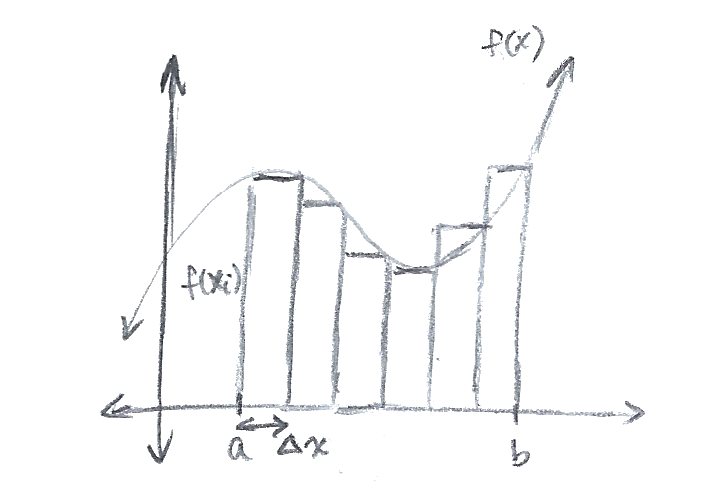
\includegraphics[scale=0.3]{images/math/calc/defintegral.png}
\end{center}
The area $A$ between the curve of $f(x)$ and $x-axis$ on the interval from $x = a$ to $x=b$ can be represented by a sum of many rectangles. If we subdivide the interval $[a,b]$ into $N$ equal intervals of length $\Delta x$, we can construct a rectangle in each interval that has width $\Delta x$ and height $f(x_i)$, where $x_i$ is the right-most $x$-coordinate of each interval. The area under the curve can be approximated by these rectangles. We can write this as:
\[
	A \approx \sum_{x_i \in [a,b]} f(x_i) \, \Delta x
\]
If we let the number of rectangles go to infinity and the width of each rectangle go to zero, we can approach the actual area of the curve. Therefore, we can write the area as a limit:
\[
	A = \lim_{N\to \infty , \Delta x \to 0} \sum_{x_i \in [a,b]} f(x_i) \, \Delta x = \int_a^b f(x) \, dx
\]
This is the definition of the definite integral, also called the Riemann integral. \\
We can also relate this to the indefinite integral. If $f(x)$ is the function that represents the rate of change of a function $F(x)$ with respect to $x$, every small rectangle in the area underneath the curve represents a small change in the value of $F(x)$. This is because that area represents the value of rate of change of $f(x)$ multiplied by the small change in $x$ ($dx$), which is the net change in $F(x)$, $\Delta F(x)$:
\[
	\Delta F(x) = f(x) \, dx
\]
If all of these small changes are summed up, the result is the net change in the function $F(x)$ on the interval $[a, b]$. Therefore, we can write the definite integral of a function $f(x)$ on the interval $[a, b]$ as the following:
\[
	\int_a^b f(x) \, dx = F(x)\Big|_a^b = F(b) - F(a) 
\] 
This is called the Fundamental Theorem of Calculus. We can now evaluate definite integrals by finding the antiderivative using an indefinite integral. This is incredibly useful for evaluating definite integrals, which we will do a lot during physics. 

\subsubsection{Differential Equations}
One of the applications for calculus is to create a model of a situation when the only information given is based on how things are changing at any particular point. Differential equations help us do this - they relate the derivatives of a function to the function itself. What if we want to do find a solution to a differential equation - that is, find an explicit expression for the function without involving its, given a few data points? This is extremely difficult in the general case, but in physics we will usually look at a few easier cases. \\
For the most part, we will be looking at first-order differential equations, where the only terms with derivatives involve the first derivative of the function. The most basic case is when the first derivative of a function only involves the independent variable $x$ (or $t$, $\theta$, etc.) and doesn't involve the function in the equation. For an example of this, let's look at the following function of $y$, assuming that we know that $y(0) = 1$:
\[
	\dv{y}{x} = e^{x} - 4x
\]
To solve it, we can just integrate with respect to $x$ from $0$ to some arbitrary real $r$: 
\[
	\int_0^r \dv{y}{x} \, dx = \int_0^r \, dy = \int_0^r e^{x} - 4x \, dx
\]
\[
	y(x)\Big|_0^r = (e^x - 2x^2)\Big|_0^r
\]
\[
	y(r) - y(0) = e^r - 2r^2 - 1
\]
\[
	y(r) = e^r - 2r^2 - 1 + y(0)
\]
Now, we see that the specific solution of the function that we're looking for depends on a data point. Since we know that $y(0) = 1$, we can simply plug in this value to get:
\[
	y(x) = e^x - 2x^2
\]
Since there's nothing special about our choice of $r$, it's simply standing in as a dummy variable - so I can replace it with $x$ or really anything I want. If I had changed the value of our initial data point, we could have had any arbitrary constant added onto the end of this, and it still would satisfy the original differential equation. In general, however, adding a constant to the end of any solution to a differential equation won't necessarily always allow it to satisfy the original equation. Let's look at another example: 
\[
	\dv{y}{x} = xy 
\]
In this case, we have the original function involved, so just integrating won't work. However, we can "separate" the variables by moving everything with a $y$ to one side and everything with an $x$ in it to another: 
\[
	\frac{1}{y} \, dy = x \, dx
\]
Now we can integrate with respect to each differential:
\[
	\ln |y| = \frac{1}{2}x^2 + C
\]
We can now solve for $y$:
\[
	y = e^{\frac{1}{2}x^2 + C} = Ce^{\frac{1}{2}x^2}
\]
Notice that because of the exponentiation, you can only manipulate the constant as a scale factor and not as an added constant. If you try substituting this back into the original equation, you can see that it works in general, whereas if you try adding a constant to the function instead it won't work. \\
In the text, I solve differential equations by moving all the terms to one side and integrating, which is essentially the same as separation of variables and results in the same solutions. Separation of variables is generally better for finding general solutions, but I use a shortcut for plugging in the data point to create the specific solution to match the situation. 

\subsubsection{Taylor Series Expansions}
The final tool that we use for solving problems are Taylor series. I claim that if a function is differentiable to an arbitrarily large degree at a point, I can approximate the behavior of the function as a polynomial at that point. (For simplicity, we'll assume that this point is at $x=0$.)\\
To create a polynomial that matches the behavior of the function at a point, all of the derivatives of the function at the point should match that of the polynomial. Let's be more specific - say the function is $f(x)$, and we know the values of $f(0), f'(0), f''(0),$ etc. We can try to build a function $p(x)$ that matches the $n$th-derivative at $x=0$. \\
If we just want to match $f(x)$ at $x=0$, we could just have $p(x) = f(0)$. This isn't a very good approximation of the function everywhere, though - it only matches the function at this point. Let's try again. \\
If we also want to make $p'(x)$ match $f'(x)$ at $x =0$, we could use a line - consider $p(x) = f(0) + f'(0) x$. Notice that this function has derivative $p(x) = f'(0)$, so it works. \\
Let's keep going to the second derivative. We want to add a term, but also make sure that the added term doesn't mess up what we had before. Because after taking two derivatives only polynomial terms of degree 2 will be constant, the added term should look like $kx^2$ for some $k$. If we take two derivatives of this term, the constant term that's left should look like $2k$ (because of the power rule). In order for us to have the right second derivative at $x = 0$, the coefficient $k = \frac{f''(0)}{2}$. So far, then, $p(x) = f(0) + f'(0)x + \frac{f''(0)}{2}x^2$ will match $f(x)$ for the first two derivatives and the value of $f(0)$. \\
We can continue on like this. The polynomial $p(x) = f(0) + f'(0)x + \frac{f''(0)}{2} x^2 + \frac{f'''(0)}{6} x^3$ will match $f(x)$ at the first three derivatives at $x=0$ (show this yourself) and we can keep adding on to infinity, basically. In general, we can make an infinite polynomial as follows that will be exactly $f(x)$:
\[
	f(x) = \sum_{i=0}^{\infty} \frac{f^{i}(0)}{i!}x^i
\]
This infinite polynomial is called the Taylor series of $f(x)$. A lot of the time, we will approximate functions using Taylor series if their inputs are close to zero. In these scenarios, we will basically just appproximate the first non-zero term to be the value of the function close to zero. Let's look at the function $\sin x$ (a function that we will approximate a lot) and compute the derivatives of $\sin x$ at $x=0$:
\[
	\sin (0) = 0
\]
\[
	\dv{}{x} \sin x = \cos x \rightarrow \dv{}{x} \sin x \Big|_{x=0} = \cos (0) = 1
\]
\[
	\ddv{}{x} \sin x = -\sin x \rightarrow \ddv{}{x} \sin x \Big|_{x=0} = -\sin (0) = 0
\]
\[
	\dnv{}{x}{3} \sin x = -\cos x \rightarrow \dnv{}{x}{3} \sin x \Big|_{x=0} = -\cos (0) = -1
\]
\[
	\dnv{}{x}{4} \sin x =  \sin x \rightarrow \dnv{}{x}{4} \sin x \Big|_{x=0} =  \sin (0) = 0
\]
Since the derivatives of $\sin x$ basically cycle through every four derivatives, we know that the Taylor series of $\sin x$ is:
\[
	\sin x = 0 + 1 \cdot x + \frac{0}{2} x^2 + \frac{-1}{6}x^3 + \frac{0}{24}x^4 + \ldots = \sum_{i = 0}^{\infty} \frac{(-1)^i}{(2i+1)!}x^{2i+1}
\]
The first non-zero term you see here is $x$, so we commonly approximate $\sin x = x$ for $x$ close to zero. (And now hopefully you understand math memes a little better.) \\
Taylor series are pretty important - although we don't use them in the text, some of the problems do require their use in order to solve them. 
\pagebreak

\subsection{Kinematics}
We begin our study of mechanics by trying to quantify the behavior of moving objects. Specifically, we will look at how objects' position, velocity, and acceleration are related, and how these can be used to solve problems involving motion, especially in certain special cases. 
\subsubsection{General Motion}
Moving forward, we will describe an object's position using a vector with respect to some point, denoted $\vec{r}$. For simplicity, we will use a point as our moving particle, but principles here really apply to any object. \\
\begin{center}
	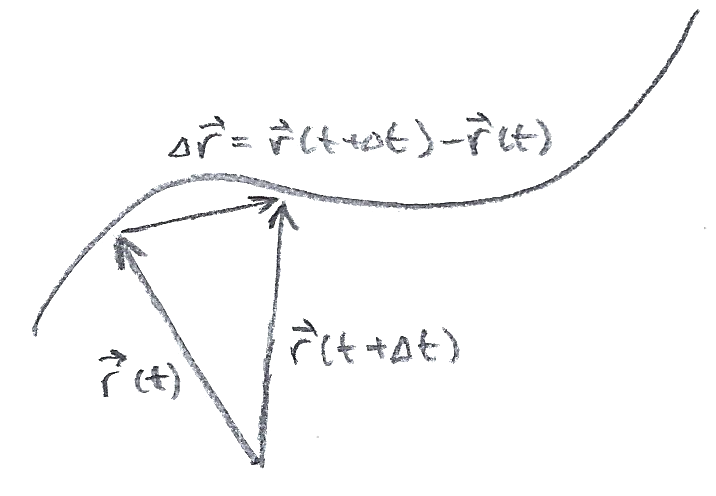
\includegraphics[width=0.5\textwidth]{images/mechintro/general_motion.png}\\
\end{center}
Knowing the position of the object is great, but we would definitely like to know more about a particle than just its position. For example, how do we know how fast is the particle going? Intuitively, we can find the average velocity of a particle over an interval by taking the distance traveled over the time interval. Consider the particle at two different times, with positions $\vec{r}(t)$ and $\vec{r}(t + \Delta t)$. Define the displacement of the particle as $\Delta\vec{r} = \vec{r}(t + \Delta t) - \vec{r}(t)$. Using the displacement vector, we can find the average velocity (a vector): 
\[
	\vec{v}_{av} = \frac{\Delta \vec{r}}{\Delta t} = \frac{\vec{r}(t + \Delta t) - \vec{r}(t)}{\Delta t}
\]
Average velocity is nice, but we would like to know the velocity instantaneously. Notice as we shrink the time interval $\Delta t$, our average velocity becomes more and more like the instantaneous velocity $\vec{v}$. In the limit as $\Delta t \rightarrow 0$, we have:
\[
	\vec{v} = \lim_{\Delta t \rightarrow 0} \frac{\vec{r}(t + \Delta t) - \vec{r}(t)}{\Delta t}
\]
This looks rather like the derivative of the position vector function $\vec{r}(t)$ with respect to time! However, we don't really know how to take the derivative of a vector, but we \textit{should} know how to take the derivative of an arbitrary function. We can actually do this by splitting the position vector $\vec{r}(t)$ into $xy$-components, where $\vec{r}(t) = x(t) \hat{x} + y(t) \hat{y}$ and $\vec{r}(t+\Delta t) = x(t+\Delta t) \hat{x} + y(t+\Delta t) \hat{y}$:
\begin{align*}
	\vec{v}(t) &= \lim_{\Delta t \rightarrow 0} \frac{x(t+\Delta t) \hat{x} + y(t+\Delta t) \hat{y} -x(t) \hat{x} -y(t) \hat{y}}{\Delta t}\\
	&= \lim_{\Delta t \rightarrow 0} \frac{x(t+\Delta t)-x(t)}{\Delta t} \hat{x} + \lim_{\Delta t \rightarrow 0}\frac{y(t+\Delta t)-y(t)}{\Delta t} \hat{y}\\
	&= \dv{x}{t}\hat{x} + \dv{y}{t} \hat{y} = v_x\hat x + v_y \hat y
\end{align*}
Note that $v_x = \dv{x}{t}$ is the $x$-component of the velocity, and $v_y = \dv{y}{t}$ is the $y$-component of the velocity. We can do this process again to attain the instantaneous acceleration vector $\vec a$, noting that the average acceleration is the change in the velocity vector over a time $\Delta t$ and allowing $\Delta t$ to go to $0$:
\[
	\vec a = \dv{v_x}{t}\hat x + \dv{v_y}{t} \hat y = \ddv{x}{t} \hat x + \ddv{y}{t} \hat y
\]
We normally don't deal with any derivatives of position (with respect to time) of order higher than two. Also, usually we will deal with constant-acceleration motion and constant-velocity (zero acceleration) motion, with some special exceptions. More general cases will be dealt with later when we discuss energy. \\
Let's deal with the constant-velocity case right now. Because of the Fundamental Theorem of Calculus, we can note the following: 
\[
	x(t) - x_0 = \int_0^t v_x \, dt = v_xt \rightarrow x(t) = v_xt + x_0
\]
where the last step follows from noting that the velocity is a constant, and therefore so are each component of the velocity vector. Using similar relations for the $y$-coordinate, we have: 
\[
	\vec r(t) = \vec v t + \vec r_0
\]
We don't need any other information about constant-velocity problems - since the velocity is constant, all higher order derivatives must be zero.\\
Now we look at the constant-acceleration case, starting with the acceleration vector $\vec a$. We can use the Fundamental Theorem of Calculus again, as we did with the constant-velocity case: 
\[
	v_x(t) - v_{0_{x}} = \int_0^t a_x \, dt = a_xt \rightarrow v_x(t) = a_xt + v_{0_{x}}
\]
Repeating this again, we can find the $x$-coordinate of position:
\[
	x(t) - x_0 = \int_0^t v_x \, dt = \int_0^t v_{0_{x}} + a_xt \, dt = v_{x0}t + \frac{1}{2}at^2  \rightarrow x(t) = x_0 + v_{0_{x}}t + \frac{1}{2}at^2
\]
Using similar processes for the $y$-coordinate, we have
\[
	\vec{r}(t) = \vec r_0 + \vec v_0 t + \frac{1}{2} \vec{a} t^2 
\]
\[
	\vec v(t) = \vec a t + \vec v_0
\]
where $\vec r_0$ is the initial position vector, $\vec v_0$ is the initial velocity vector, and $\vec a$ is the acceleration vector. \\
These equations work fine unless we don't have access to time data. However, we can derive a constant-acceleration equation that does not involve time, using one dimension for simplicity. We can square our general equation for velocity: 
\begin{align*}
	v &= at + v_0 \\
	v^2 &= a^2t^2 + v_0^2 + 2atv_0 \\
	v^2 - v_0^2 &= 2a\left(\frac{1}{2}at^2 + v_0t \right)
\end{align*}
This expression in the parentheses is familiar - note the displacement can be written as:
\[
	\Delta x = x(t) - x_0 = \frac{1}{2}at^2 + v_0t
\]
Now we have a kinematic equation that does not deal with time: 
\[
	v^2 - v_0^2 = 2a\Delta x
\]
Note that these equations are the same in higher dimensions (for example, in 3D space) and are derivable with the same procedures and steps. 

\subsubsection{Circular Motion}
A special type of motion that we will study is circular motion. In order to derive the equations for this motion, we use polar coordinates. We can parameterize the points in the plane with the angle it makes with the positive $x$-axis and the distance from the origin. Let $\theta(t)$ be this angle as a function of time, and we can express the position of a point in the plane as $\vec r = r \cos (\theta (t)) \, \hat x + r \sin (\theta (t)) \, \hat y$, where $r$ is the constant radius of the circle the particle travels upon. In addition to $\hat x$ and $\hat y$, constant unit vectors, we define changing unit vectors $\hat r$ and $\hat \theta$, where $\hat r$ is radially outward and $\hat \theta$ is the unit vector perpendicular to it, defined as follows: \\
\[
	\hat r = \cos (\theta (t)) \, \hat x + \sin (\theta (t)) \, \hat y 
\]
\[
	\hat \theta = -\sin (\theta (t)) \, \hat x + \cos (\theta (t)) \, \hat y
\]
\begin{center}
	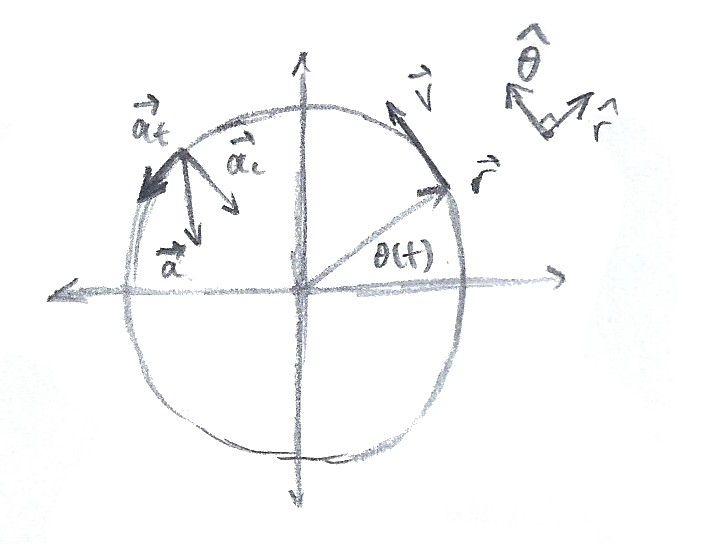
\includegraphics[width=0.5\textwidth]{images/mechintro/circular_motion.png}\\
\end{center}
We can take the derivative of the position vector in order to find the velocity of the object, using the method in the previous section: 
\[
	\vec v = \dv{\vec r}{t} = - r \sin (\theta (t)) \, \dv{\theta}{t} \, \hat x + r \cos (\theta (t)) \, \dv{\theta}{t} \, \hat y
\]
Notice by the chain rule an extra $\omega = \dv{\theta}{t}$ appears in each term; this term is called the angular velocity. We can rewrite $\vec v$ as follows: 
\[
	\vec v = \omega r (-\sin (\theta (t)) \, \hat x + \cos (\theta (t)) \, \hat y) 
\]
The acceleration of the object is a bit messy, but we can take derivatives again, substituting $\alpha = \dv{\omega}{t}$: 
\begin{align*}
	\vec a = \dv{\vec v}{t} &= -r \left(\dv{\omega}{t}\sin (\theta (t)) + \omega^2 \cos (\theta (t)) \right) \hat x + r \left(\dv{\omega}{t} \cos (\theta (t)) - \omega^2 \sin (\theta (t)) \right) \hat y \\
	&= \alpha r (-\sin (\theta (t)) \, \hat x + \cos (\theta (t)) \, \hat y) - \omega^2 r (\cos (\theta (t)) \, \hat x + \sin (\theta (t)) \, \hat y) 
\end{align*}
This is all pretty messy, but we can clean up these expressions by using $\hat r$ and $\hat \theta$: 
\begin{align*}
	\vec r &= r \hat r \\
	\vec v &= \omega r \hat \theta \\
	\vec a &= \alpha r \hat \theta - \omega^2 r \hat r
\end{align*}
Observe that since these unit vectors have magnitude $1$, so the velocity $v = \omega r$, with direction tangent to the circle. We should notice for cases with non-constant acceleration, we have a centripetal component ($-\omega^2 r \hat r$, pointing radially inward) and a tangential component ($\alpha r \hat \theta$, tangent to the circle).
A special case we study is when $\omega$ is a constant, implying that $\alpha = 0$. This is called uniform circular motion, and we see for this case the only acceleration is centripetal: 
\[
	\vec a = - \omega^2 r \hat r = - \frac{v^2}{r} \hat r 
\]
Overall, we have, for uniform circular motion (for the magnitudes of the velocity and angular velocity):
\begin{align*}
	v &= \omega r \\
	a &= \omega^2 r = \frac{v^2}{r}
\end{align*}

\subsubsection{Simple Harmonic Motion (SHM)}
Consider projecting circular motion into one dimension - namely, only considering the $x$-direction. This one-dimensional motion can basically be modeled by the function $x(t) = A \cos(\omega t + \phi)$, where $A$ is the amplitude, $\omega$ is the frequency/angular velocity, and $\phi$ is the phase shift. This is simple harmonic motion, which essentially uses a sine/cosine function as a model for motion. \\
Using our knowledge of derivatives, the velocity and acceleration functions: 
\begin{align*}
	v(t) &= -\omega A \sin(\omega t + \phi) \\
	a(t) &= -\omega^2 A \cos(\omega t + \phi) 
\end{align*}
We'll do something somewhat unorthodox - we'll substitute $x(t)$ for the cosine function in the acceleration function, giving: 
\[
	a(t) = \ddv{x}{t} = -\omega^2 x(t)
\]
In general, if given an acceleration function proportional to position, where $a(t) = -kx(t)$, we know the particle exhibits simple harmonic motion (sine/cosine wave) where $\omega = \sqrt{k}$ and the period $T = \frac{2\pi}{\omega} = \frac{2\pi}{\sqrt{k}}$. \\
Mathematically, if a second derivative of a function $\ddv{f}{t} = -kf$, the function $f$ can be modeled as a sine or cosine function. 

\subsubsection{Projectile Motion and Relative Motion}
We can apply general 2-D motion principles to projectiles. Let a particle be launched at an angle $\theta$ at an initial velocity $v_0$. Note that this particle is constantly accelerating downward with magnitude $g = 9.81 \, m/s^2$. To make things simpler, we will automatically project into the $x$- and $y$- directions, with the implication that we are in fact dealing with vectors. Also, further assumptions that we make is that the Earth's gravitational acceleration is uniform at all heights - which clearly isn't true in outer space - but otherwise we have non-constant acceleration which we haven't learned to deal with yet. We also neglect air resistance, which changes the acceleration of the particle. \\
The initial velocity in the $x$-direction is $v_0 \cos \theta$, and the initial velocity in the $y$-direction is $v_0 \sin \theta$. Plugging into our derived time-dependent kinematic equations, and letting the initial position be the origin: 
\[
	x(t) = v_0t\cos\theta  \quad v_x(t) = v_0\cos\theta
\]
\[
	y(t) = v_0t\sin\theta  - \frac{1}{2}gt^2 \quad v_y(t) = v_0 \sin \theta - gt
\]
We can analyze some critical points - we can calculate how far the particle will travel before it hits the ground, namely when $y = 0$. When this is the case, we have: 
\[
	v_0t\sin\theta  - \frac{1}{2}gt^2 = 0 \rightarrow v_0\sin\theta - \frac{1}{2}gt = 0
\]
This equation has a zero when $t=0$, and solving the remaining linear equation yields $t = \frac{2v_0\sin\theta}{g}$. When this is plugged into $x(t)$, we have $\frac{2v_0^2\sin\theta \cos\theta}{g} = \frac{v_0^2\sin 2\theta}{g}$.\\
Similarly, we can consider when the particle reaches its maximal height. Clearly, by symmetry we have that the distance that the particle had traveled to that point is $\frac{v_0^2\sin \theta \cos\theta}{g}$. However, we can find the maximal height by calculating the time when the $y$-component of the velocity is $0$, where the particle stops going upward and begins to fall back to earth. This occurs when:
\[
	v_0\sin\theta - gt = 0 \rightarrow t = \frac{v_0\sin\theta}{g}
\]
Note that the time when this occurs is exactly half of the time it takes for the particle to hit the ground. When this occurs, the height can be calculated by plugging into $y(t)$, where $y(t) =\frac{v_0^2\sin^2\theta}{2g}$. \\
Of course, this is all well and good, but we do need to be able to consider when things hit each other, especially with projectiles (which is a very common problem). \\
\begin{center}
	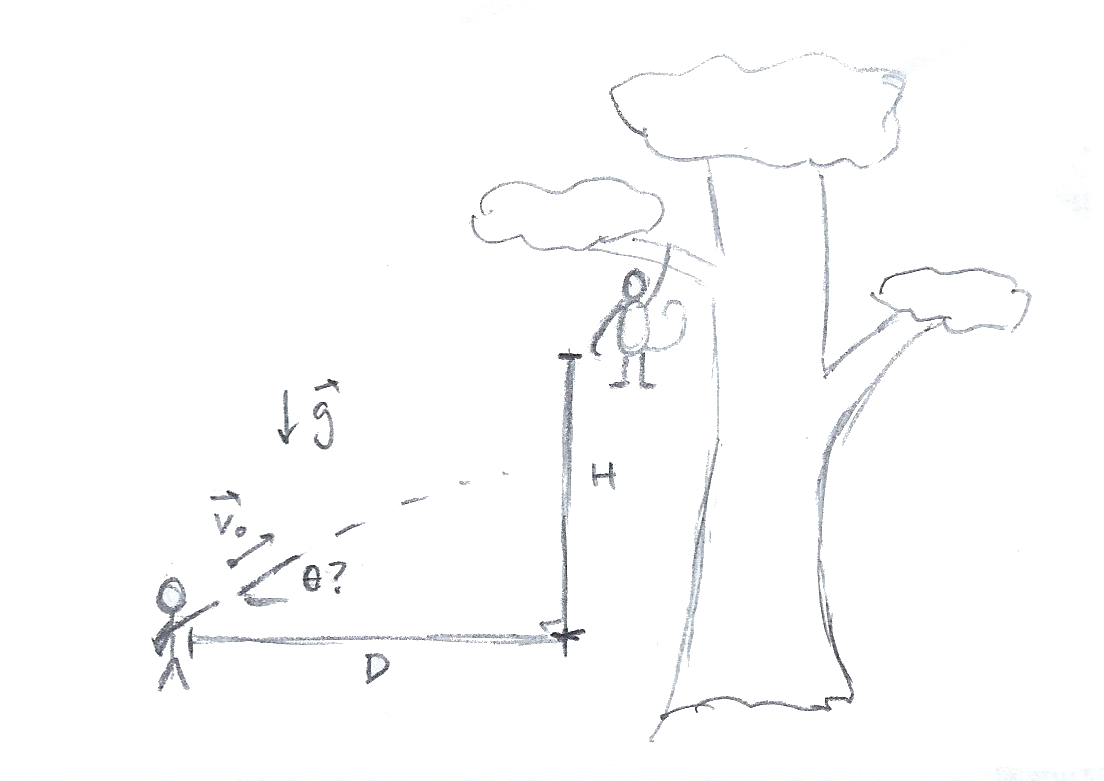
\includegraphics[width=0.5\textwidth]{images/mechintro/projectile_motion.png}\\
\end{center}
We can use kinematics to solve problems - one of the first applications was used for hunting, because animal cruelty organizations didn't exist when physics was invented. For example, suppose a hunter stands a distance $D$ away from the base of a tree, in which a monkey is sitting at the top, hanging from a branch. The monkey is hanging at a height $H$, and the hunter can shoot a bullet at the monkey with velocity $v_0$. We're trying to find at what angle $\theta$ should the hunter fire to hit the monkey. We're also assuming the monkey is effectively a point, and at the instant the hunter fires, the monkey lets go of the branch and begins to fall freely with downward acceleration with magnitude $g$.\\
Consider the position vector of the monkey relative to the bullet, $\vec r_{MB}$. To deal with this, we employ the following, where $O$ is some arbitrary origin we've been using the entire time:
\[
	\vec r_{BO} + \vec r_{MB} = \vec r_{MO} \rightarrow \vec r_{MB} = \vec r_{MO} - \vec r_{BO} 
\]
To compute the relative position vector, then, we really only need to 
compute the position vectors of the monkey and the bullet and subtract them. We know they collide when their relative position vector is the zero vector $\vec 0$.  We know how both of these particles work - effectively, they are both projectiles, which we have just established. For simplicity, let the position of the hunter be the origin. Then, we have: 
\[
	\vec r_{MO} = D\, \hat x + \left(H - \frac{1}{2}gt^2 \right)\, \hat y \quad \vec r_{BO} = v_0t\cos\theta \, \hat x + \left(v_0t\sin\theta - \frac{1}{2} gt^2 \right) \, \hat y
\]
Then their relative position is: 
\[
	\vec r_{MB} = (D - v_0t\cos\theta) \, \hat x + (H - v_0t\sin\theta) \, \hat y
\]
When this is the zero vector, we have that both components are zero, giving:
\[
	\cos \theta = \frac{D}{v_0t} \quad \sin \theta = \frac{H}{v_0t} \rightarrow \tan \theta = \frac{H}{D}
\]
This angle is the exact angle at which the hunter should shoot the monkey hanging from the tree, given our assumptions. Therefore, the hunter should aim directly at the monkey, as long as the bullet is traveling fast enough to reach the tree before the monkey hits the ground. 

\subsubsection{Summary and Problems}
Position, velocity, and acceleration of objects can be represented by a vector with respect to a point. Velocity is the derivative with respect to time of position, and acceleration is the derivative with respect to time of velocity (and the second derivative with respect to time of position). Position and velocity can be attained through velocity or acceleration functions, respectively, through integration. \\
We deal with a few special cases, being (uniform) circular motion, simple harmonic motion, and projectile motion. These are situations that we should be proficient in before moving forward to more complex motion and systems. \\

\noindent \textbf{Problems:}\\
1. (3 $\bigstar$) At $1/2$ of its maximum height, the speed of a projectile is $3/4$ of its initial speed. If the particle was initially launched at an angle $\theta$, where $\theta = \arctan(x)$, show that $x = \sqrt{7}$.\\
2. (2 $\bigstar$) A boy whirls a stone in a horizontal circle of radius $r$ and at height $h$ above ground level. The string breaks, and the stone flies horizontally and strikes the ground after traveling a horizontal distance of $d$. Show the magnitude of the centripetal acceleration of the stone while in circular motion is $d^2g/2hr$. \\
3. (2 $\bigstar$) Two particles oscillate in simple harmonic motion along a common straight-line segment of length $A$. Each particle has a period of 3.80 s, but they differ in phase by $\pi/8$ rad. a) Show the maximum acceleration and velocities of the particles are 2.734$A$ and 1.653$A$, respectively. b) Show the particles are 0.167$A$ apart $0.50$ s after the lagging particle leaves one end of the segment.\\
4. (1 $\bigstar$) A tank fires a rocket at a velocity $v_r$ at an angle $\theta$ above the horizontal. Immediately afterward, the tank begins moving forward at a constant speed $v_t$. Show that the angle of stupidity $\theta$ of the tank - that is, the angle at which the rocket will fall down to strike the tank while on the ground - as $\arccos(v_t/v_r)$. \\
5. (3 $\bigstar$, $\spadesuit$) A small rock sinking through water experiences an exponentially decreasing acceleration given by $a_y(t) = ge^{-bt}$, where $b$ is a positive constant that depends on the shape/size of the rock and the properties of the water. If the initial position and velocity of the rock are both zero, find the a) velocity function to be $v_y(t) = \frac{g}{b} (1-e^{-bt})$. b) the position function to be $y(t) = \frac{g}{b}t - \frac{g}{b^2}(1-e^{-bt})$.\\
6. (2 $\bigstar$) Prove that if two particles are launched at the same speed $v_0$ but at angles above the horizontal that exceed/fall short of 45 degrees by the same amount, they will still travel the same distance (on level ground).\\
7. (3 $\bigstar$) If two balls are thrown with the same initial speed $v_0$ but at different angles $\alpha$ and $\beta$ above and below the horizontal, respectively, and from a cliff a height $h$ above the ground, show that their velocities right before they hit the ground are the same and is equal to $v = \sqrt{v_0^2+2gh}$.\\

\pagebreak

\subsection{Dynamics and Newton's Laws}
Once we have the tools to deal with motion to some level, we now begin to deal with how interactions between objects influence motion - specifically, with the use of forces. Forces have units of kg $\cdot$ m/s$^2$, also denoted as N, called the newton in honor of Isaac Newton. One newton (1 N) of force is the amount needed to accelerate a 1 kg mass by 1 m/s$^2$. 
\subsubsection{The Laws of Motion}
When Newton developed his theory of dynamics for the first time, he established the quantity of linear momentum, $P$, representing the motion of a mass particle. He defined it as:
\[
	\vec P = m \vec v
\]
Forces, he said, were the flow of linear momentum in between objects in contact. Objects in contact with each other are interacting, delivering this momentum to each other. These forces can be represented as vectors, delivering this momentum from place to place. \\
With this in mind, this means force is the derivative of the linear momentum with respect of time, and we obtain the iconic second of Newton's three laws of motion, regarding all forces acting on a particle:
\[
	\sum_i \vec F_i = \dv{\vec P}{t} = m \dv{\vec v}{t} = m \vec a
\]
However, we have to be careful about how we use this law. In physics, since we can't analyze the whole universe in one go, we only look at subsections of the universe called reference frames, from which we can analyze the physical situation. If a reference frame has any added external forces to a system, they will change the motion of an object within - this is Newton's first law. An object's velocity, whether at rest or positive, will be changed by the addition of an external force. This means that in order to maintain consistency, we cannot analyze objects that lie in reference frames that are accelerating and expect them to be consistent with the results obtained from a stationary measurement since some external force is causing them to accelerate. Therefore, we only analyze objects in inertial reference frames, that is, a reference frame that does not change the inertia or momentum of the system. \\
To illustrate this, let's imagine Dr. Dell in his brand-new Tesla, on the highway. He accelerates, and as he does so, he notices sheep, standing in a pasture, as he passes by. Relative to him, Dr. Dell sees the sheep accelerating backward, and concludes there must be some force in that direction that makes them move this way. However, if I stand next to these sheep in the field, clearly I see them at rest. The laws of physics do not apply arbitrarily, in order to maintain a consistent image of the universe.\\
Forces primarily come from objects that come into contact with one another. When two objects interact, they exert forces on each other, and they do so with equal magnitude in opposite directions. This is Newton's third law, the establishment of the existence of these forces called action-reaction pairs. For example, if a book is sitting on a table, the book is exerting a downward force on the table, but the table is also exerting an upward force on the book. However, the force of gravity on the book is not an action-reaction pair with the upward force from the table! Even though the two forces are opposite in direction and have the same magnitude, gravity is a result of an interaction with the Earth, which means it cannot be paired with the force from the table.\\
To briefly sumamrize Newton's Laws of Motion: 
\begin{mdframed}[frametitle=Newton's Laws of Motion]
	1. In a system with no internal forces, an object's velocity can only be changed by some external force.\\
	2. Force is the flow of linear momentum between objects, and thus forces on an object have the same direction as the net acceleration of an object.\\
	3. Particles that interact with each other have forces exerted on each other that are opposite in direction but equal in magnitude. 
\end{mdframed}
Not only are there contact forces, however, there are also action-at-a-distance forces that we have not yet considered. These also follow Newton's Second Law but seem to come from nowhere (a problem that we still don't really know the answer to today!). We include them when drawing free-body diagrams, where we list all the possible forces that act on an object, such as gravity, the electromagnetic force (discussed in length later), and the strong and weak nuclear forces (not discussed). In mechanics, we mostly concern ourselves with gravity, a largely macroscopic force. In problems that are assumed to be on Earth, gravity does exert an external force on the system, so strictly speaking, the Earth is not an inertial frame! However, we will still apply Newton's laws in these systems, and just automatically consider gravity acting on the system where applicable. 
\subsubsection{The Sandbox}
In many problems, certain common objects occur in systems that have well-known properties that students must know in AP Physics. 
\begin{mdframed}[frametitle=The Gravitational Force]
	Earth exerts an action-at-a-distance force on all objects on its surface. This force has magnitude $mg$, where $m$ is the object's mass, $g$ is the acceleration due to gravity ($9.81 m/s^2$) and is directed straight down.
\end{mdframed}
\begin{mdframed}[frametitle=The String and The Tensile Force]
	For ideal strings that are effectively massless, and stretched taut, the tension in the string acts as a contact force on the object in the direction of the string outward from the object. The magnitude of this force is the same for all objects attached to the string. 
\end{mdframed}
\begin{mdframed}[frametitle=The Normal Force]
	The contact force from a surface exerted on an objects when touching each other perpendicular to the surface. It is part of an action-reaction pair with force from the object on the surface, but not with the force of gravity on the object. 
\end{mdframed}
\begin{mdframed}[frametitle=The Frictional Force]
	A contact force that opposes the motion of objects. Friction comes in two types - static friction and kinetic friction. \\
	Static friction is for objects at rest and has a magnitude $f_s \leq \mu_sN$, where $N$ is the magnitude of the normal force and $\mu_s$ is the coefficient of static friction (between $0$ and $1$). This force opposes an applied force on an object until the magnitude of this force exceeds the maximum magnitude of the static frictional force, at which point the object will begin to move.\\
	Kinetic friction opposes the motion of a moving object and has magnitude $f_k = \mu_kN$, where $\mu_k$ is the coefficient of kinetic friction (also between 0 and 1, usually smaller than $\mu_s$). This force points in the exact opposite direction of the velocity of the object to decelerate the object. 
\end{mdframed}
\begin{mdframed}[frametitle=The Elastic Force]
	The elastic force, usually exerted by a spring in problems, has magnitude $\vec F_{spring} = -k \Delta \vec x$, where $\Delta \vec x$ is the displacement of the object attached to the spring from equilibrium, and $k$ the spring constant. Note that this force opposes compression/stretching of the spring. Without any other forces on this system, objects attached to a spring move in simple harmonic motion. 
\end{mdframed}
\begin{mdframed}[frametitle=The Drag Force]
	The force of drag on an object is $F_d = \beta v^n$, where $\beta$ is the coefficient of drag, $v$ is the velocity, and $n$ is some arbitrary real ($n=2$ through air and many other fluids). This force opposes motion through the air, and we usually don't consider this force because it has a negligible impact on results on the scale of the lab. 
\end{mdframed}
\subsubsection{Atwood's Machine}
The most common example that requires the application of Newton's Laws is Atwood's machine, which is essentially a pulley with two masses hanging from both ends of a string wrapped around it. The string does not slip on the pulley and is effectively massless, and for now, the pulley is fixed and does not rotate with the string (this is a non-trivial constraint that we will talk about later). \\
\begin{mdframed}[frametitle=Atwood's Machine]
Consider Atwood's machine with masses $m_1$ and $m_2$, and $m_2 > m_1$. Find the acceleration of the blocks and the tension in the string in terms of $m_1, m_2, g$, where $g$ is the acceleration due to gravity.
\end{mdframed}
The first thing we need to do is figure out what forces are acting on both blocks. We're not considering air resistance, and no friction is acting between the pulley and the string, so we can ignore these contact forces. The most helpful tool we use in these problems is a free-body diagram, which illustrates the forces acting on each object. Here are the free body diagrams for both of the blocks: 
\begin{center}
	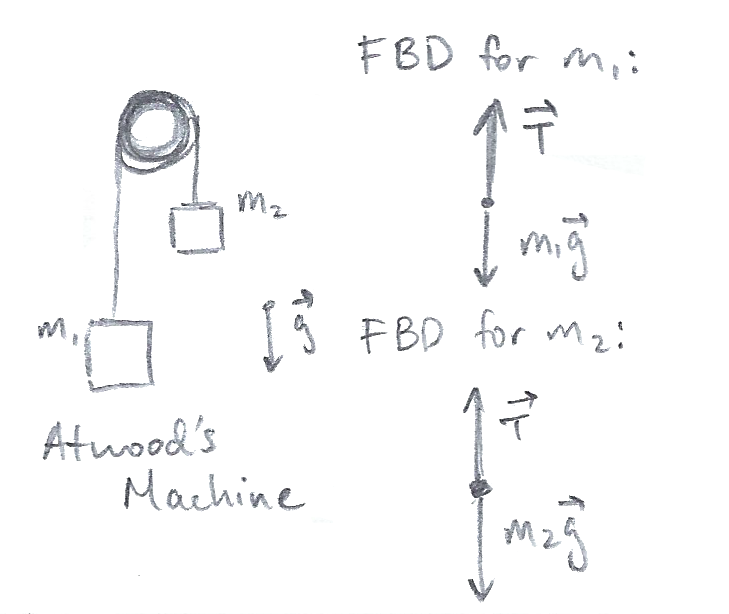
\includegraphics[width=0.5\textwidth]{images/mechintro/atwoods_machine.png}\\
\end{center}
Note that the forces only act in one direction, so we will establish a unit vector $\hat y$ upwards in order to project the components of the forces along this line. First, we do need to write Newton's Second Law for each block: 
\[
	\sum_i \vec F_i = m_1 \vec g + \vec T = m_1 \vec a
\]
\[
	\sum_i \vec F_i = m_2 \vec g + \vec T = -m_2 \vec a
\]
The only subtlety here is noting that kinematically, the blocks are attached to each other and thus have the same acceleration, except in opposite directions - when one goes up, the other must go down, and vice versa, resulting in a negative sign in front of one of the equations. \\
Now we can project along the $y$-direction:
\begin{align*}
-m_1g + T = m_1a \\
-m_2g + T = -m_2a
\end{align*}
This is a two-variable system of equations with two unknowns, so we can just solve for $T$ and $a$, which aren't particularly pretty, but are:
\[
	T = \frac{2m_1m_2}{m_1+m_2}g \quad a = \frac{m_2-m_1}{m_2+m_1}g
\]

\subsubsection{Summary and Problems}
Newton's laws of motion can be applied to situations to analyze how objects move, especially when external forces are applied to systems of objects. We also can start to figure out how objects interact with each other based on their contacts with one another. \\
There isn't much to do other than to practice the method we use to analyze dynamical situations, that being to draw correct free-body diagrams, using Newton's Second Law and projecting into components, and then solving for all unknowns using some kinematics to simplify the number of variables involved.  \\

\noindent \textbf{Problems}\\
1. (1 $\bigstar$) a) A block of mass $m$, experiencing a force of friction, slides at constant speed down a plane inclined at an angle $\theta$ with the horizontal. Show $\mu_k = \tan\theta$. b) The same block rests on a frictionless wedge inclined at an angle of $\theta$. If the wedge is accelerated with acceleration $\vec a$ so that the block remains stationary relative to the wedge, show that the magnitude of this acceleration is $a = g\tan \theta$. \\
2. (3 $\bigstar$) A stone of mass $m$ attached to a string is whirled in a horizontal circle of radius $r$. The string makes an angle of $\theta$ with the vertical, and the other end of the string is fixed directly above the center of the circle. Show the speed of the stone is $v = \sqrt{rg\tan\theta}$ and the tension in the string is $T = mg/\cos\theta $.\\
3. (2 $\bigstar$) A slide-loving pig slides down a side with angle $\theta$ in $n$ times the time it would take to slide down a frictionless slide with angle $\theta$. Show that the coefficient of kinetic friction between the pig and the first slide is $\frac{n^2-1}{n^2}\tan\theta$.\\
4. (3 $\bigstar$) A puck of mass $m$ slides in a circle of radius $r$ on a frictionless table while attached to a hanging cylinder of mass $M$ by a cord through a hole in the table. Show if that the cylinder is to remain at rest, the puck needs to be moving at a speed of $v = \sqrt{\frac{Mgr}{m}}$. \\
5. (3 $\bigstar$, $\spadesuit$) Revisit Atwood's machine, in which two containers are connected by a cord (of negligible mass) passing over a frictionless pulley (also of negligible mass). At time $t = 0$, container 1 has mass 1.30 kg and container 2 has mass 3.36 kg, but container 1 is losing mass (through a leak) at the constant rate of 0.256 kg/s. a) Show that the rate at which the acceleration magnitude of the containers changing at $t = 3.00 \, s$ is 1.11 m/s$^3$. b) Show the acceleration reaches its maximum value at $t = 5.08$ s.\\
6. (2 $\bigstar$) The floor of a railroad flatcar is loaded with loose crates having a coefficient of static friction $\mu_s$ with the floor. If the train is initially moving at a speed of $v$, show the minimum distance $\Delta x$ in which the train can be stopped at constant acceleration without causing the crates to slide over the floor is $\frac{v^2}{2g\mu_s}$.\\
7. (5 $\bigstar$) A car travels on a banked curve. The coefficient of static friction between the tires of the car and the roadway of the banked curve is $\frac{3}{4}$. The curve has radius $R$ and is banked at the incline angle so that the force of static friction is zero if the car travels with constant speed $S$. Show that the maximum speed that a car can traverse the banked curve is $SRg \sqrt{\frac{7}{4-3S^2}}$. 

\pagebreak

\section{Conserved Quantities}
Aside from basic tools such as Newton's Laws or kinematics, when certain events occur we can analyze them using the conservation of certain physical quantities. This involves the use of linear momentum (that which forces are carriers of), angular momentum, and energy.

\subsection{Linear Momentum}
We mentioned linear momentum a bit in our discussion about forces, defining the product of an object's mass and velocity to be this quantity, as follows: 
\[
	\vec P = m \vec v
\]
where $\vec P$ stands for linear momentum. This is a vector quantity and has the same direction as the velocity and units of kg $\cdot$ m/s = N $\cdot$ s. 
\subsubsection{Impulse-Momentum Theorem}
Impulse is something that often comes up with discussions of linear momentum, and it would seem at first like a completely separate quantity. The impulse delivered to an object $\vec J$, in terms of the net force $\vec F$ on it over a time interval $[t_1, t_2]$ is defined to be the following: 
\[
	\vec J = \int_{t_1}^{t_2} \vec F \, dt
\]
Recall we can write the force $\vec F = \dv{\vec P}{t} = m \vec a$, so this becomes:
\[
	\vec J = \int_{t_1}^{t_2} \dv{\vec P}{t} \, dt = \vec P(t_2) - \vec P(t_1) = \Delta \vec P
\]
So, impulse is nothing terribly special - it's equal to the change in linear momentum delivered to a particle. This is also true in general for systems of particles - the total impulse delivered to a system is equal to the change in the total linear momentum of the system. This is the Impulse-Momentum Theorem, relating impulse to linear momentum. \\
We can go one step further. Notice that the average force on an object $\vec F_{av}$ is
\[
	\vec F_{av} = \frac{\Delta \vec P}{\Delta t}
\]
so the impulse delivered to the system over a time $\Delta t$ is just 
\[
	\vec J = \vec F_{av} \Delta t
\]
\subsubsection{Center of Mass}
The center of mass is a tool we need to use in order to use momentum effectively. From up until this point we have been operating under the assumption that objects effectively behave like a point particle. This really isn't true - after all, something like a baton when thrown into the air spins, and the motion of the end of the baton does not follow a perfect parabolic path as kinematics would have us believe. However, we know for certain that one point in the baton system follows this parabolic trajectory, being the center of mass. \\
First, let's just define the center of mass of a system of particles. Say with respect to some reference point these particles have position vectors $\vec r_i$, where $i$ goes from $1$ to however many particles there are. If each particle also has a mass $m_i$, and the mass of all of the particles is $M$, then the position of the center of mass $\vec r_{cm}$ is: 
\[
	\vec r_{cm} = \frac{1}{M} \sum_i m_i\vec r_i
\]
Essentially, this is a weighted average of the positions of each particle with respect to the mass. Since the masses are all scalars, we can take derivatives to find the velocity and acceleration of the center of mass, showing that these can also be found by taking the mass-weighted average of all the velocities and accelerations, respectively, of the particles. 
\[
	\vec v_{cm} = \dv{\vec r_{cm}}{t} = \dv{}{t} \frac{1}{M} \sum_i m_i \vec r_i = \frac{1}{M} \sum_i m_i \dv{\vec r_i}{t} = \frac{1}{M} \sum_i m_i \vec v_i
\]
\[
	\vec a_{cm} = \dv{\vec v_{cm}}{t} = \dv{}{t} \frac{1}{M} \sum_i m_i \vec v_i = \frac{1}{M} \sum_i m_i \dv{\vec v_i}{t} = \frac{1}{M} \sum_i m_i \vec a_i
\]
So how to find the center of mass? For a discrete collection of particles, the calculations are fairly straightforward - one just projects into components, and uses the same mass-weighted average to find the $x$-, $y$-, etc. components of the center of mass. Putting it all together with appropriate unit vectors gives the correct position vector. \\
For continuous distributions of mass, we have to be a bit more clever. If we let the mass of each little particle/subsection in a larger object go to zero as we divide it up into smaller and smaller pieces, then we can compute the desired sum as an integral by summing together all the appropriate pieces. This gives us:
\[
	\vec r_{cm} = \frac{1}{M} \int \vec r \, dm
\]
where $\vec r$ is the position vector of each infinitesimally small mass portion $dm$. 
Usually, when computing the center of mass for continuous distributions we define a density function $\lambda$, which represents mass per unit length. (AP Physics doesn't require being able to compute the center of mass for two/three/higher dimensional objects.) As a basic example, a rod with uniform density and mass $M$ and length $L$ has its center of mass in the middle of the rod, by symmetry. As a more nontrivial example, consider a semicircle with radius $R$ and uniform density (mass per unit length) $\lambda$.
\begin{center}
	\begin{asy}
		import olympiad;
		pair O, P, X;
        size(8cm);
		O = (0,0);
		dot(O);
		draw(arc(O, 1, 0, 180));
		real dtheta = 8;
		real angle = 40;
		X = dir(angle);
		P = dir(angle+dtheta);
		draw(O--P, linetype("8 8"));
		draw(O--X, linetype("8 8"));
		real vertoffset = -0.1;
		draw((0, vertoffset)--(-1, vertoffset), linetype("8 8"), arrow=Arrows());
        draw(dir(180)--dir(0), linetype("4 4"));
        draw(arc(O, 0.8, angle, angle+dtheta), arrow=Arrows());
        dot(2*dir(90)/pi);
        
        label("$\theta$", 0.15*dir(angle/2), dir(angle/2));
        label("$ds$", dir(angle+dtheta/2), dir(angle+dtheta/2));
        label("$R$", (-0.5, 1.2*vertoffset), dir(270));
        label("$d\theta$", 0.7*dir(angle-dtheta), dir(angle-dtheta));
        label("COM", 2*dir(90)/pi, NW);
	\end{asy}
\end{center}
Because the semicircle is uniform, we know that $\lambda = \frac{M}{\pi R}$, but we're not going to plug it into our expressions until the end. Let the $x$-axis be the diameter of the semicircle, and the $y$-axis the line through the center perpendicular to it. From here, we're going to use polar coordinates. \\
The vector $\vec r$ for all points on the semicircle is $R \cos \theta \, \hat x + R \sin \theta \, \hat y$, as $\theta$ ranges from $0$ to $\pi$. Now, we have to express $dm$ in terms of $\theta$. Note since each small piece is a small arc of the semicircle, $dm = \lambda \, ds$, where $ds$ is a small arc. We know that $ds = R \, d\theta$, so at the end of the day we have $dm = \lambda R \, d\theta$. Now, we can integrate and evaluate: 
\begin{align*}
	\vec r_{cm} &= \frac{1}{M} \int \vec r \, dm\\
	&= \frac{1}{M} \int_0^\pi \lambda R (R \cos \theta \, \hat x + R \sin \theta \, \hat y) \, d\theta \\
	&= \frac{\lambda R^2}{M} \int_0^\pi \cos \theta \, \hat x + \sin \theta \, \hat y \, d\theta \\
	&= \frac{\lambda R^2}{M} \left( \int_0^\pi \cos \theta \, d\theta \, \hat x + \int_0^\pi \sin \theta \, d\theta \, \hat y \right)\\
	&= \frac{\lambda R^2}{M} \left( \sin \theta \Big |_0^\pi \hat x - \cos \theta \Big|_0^\pi \, \hat y \right)\\
	&= \frac{2}{\pi}R \, \hat y
\end{align*}
Notice that we could have simplified our calculations a little bit, since we would have only needed to consider the $y$-component because the $x$-component would've come out to be $0$ by symmetry. This result is also a bit strange, in that the center of mass doesn't actually lie on the actual body of mass, but the result is in fact correct. A similar procedure to what we've done here can be applied to other continuous mass distributions and even non-uniform bodies given the density function $\lambda$.

\subsubsection{Conservation of Linear Momentum}
The center of mass of a system of particles may seem clunky to use or not quite connected to what we've done so far, but we can connect it to what we've established so far about dynamics. \\
The sum of all the forces on all the particles in a system is the following, by Newton's Second Law: 
\[
	\sum_i \vec F_i = \sum_i m_i \vec a_i 
\]
We can divide up these forces into those that are external to the system, and those that are internal to the system and multiply/divide on the right-hand side by the total mass $M$: 
\[
	\vec F_{net}^{int} + \vec F_{net}^{ext} = M \frac{1}{M}\sum_i m_i \vec a_i 
\]
Notice, however, that by Newton's Third Law, the internal forces are all part of action-reaction pairs, which all sum to zero. Therefore, we can eliminate that term. Furthermore, we can substitute in the acceleration of the center of mass $\vec a_{cm}$:
\[
	\vec F_{net}^{ext} = M \vec a_{cm} = \dv{\vec P_{sys}}{t}
\]
This is a more general form of Newton's Second Law, but for a system of particles rather than just a singular point particle. Similarly, by integrating this in the same way as before, the total linear momentum of the system $\vec P_{tot}$ is:
\[
	\vec P_{tot} = M \vec v_{cm}
\]
What if the sum of the external forces on a system is zero? Then the linear momentum of the system $\vec P_{tot}$ is some constant. To be clear: 
\begin{mdframed}[frametitle=Conservation of Linear Momentum]
For a system with no external forces, linear momentum is conserved - the amount of linear momentum in the system remains constant and is not changed by the internal motion/dynamics of the system.
\end{mdframed}
\subsubsection{Rockets}
We're going to apply concepts of linear momentum to derive the rocket equation in one dimension. (This isn't part of the AP course, but it might show up on an exam.) In the most abstract sense, rockets shoot mass out their end to propel themselves forward, which usually takes the form of fuel (but Dr. Dell suggested using a cuter power source, such as having gerbils jump off the end).\\
\begin{center}
	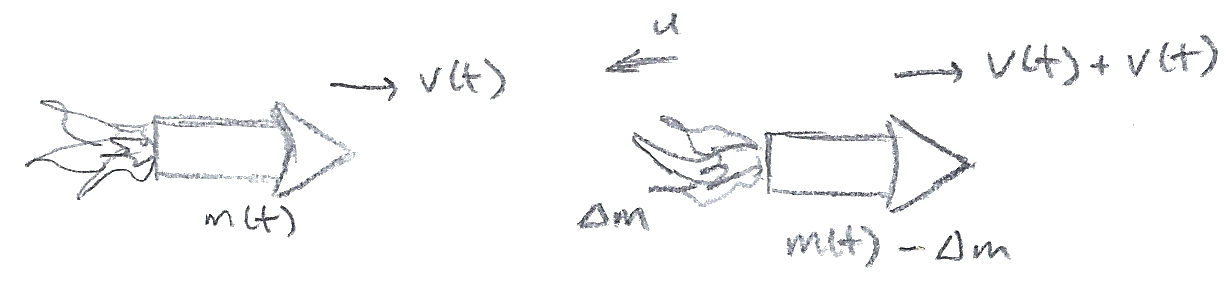
\includegraphics[width=0.5\textwidth]{images/mechintro/rockets.png}\\
\end{center}
To set this up, let $m(t)$ be the mass of the rocket as a function of time, $v(t)$ be the velocity (in one dimension, for simplicity) and $u$ be the exhaust velocity, or how fast the mass being shot out the back end is going. \\
Since we're assuming no external forces are acting on the system, we can apply conservation of linear momentum. At some time $t$, we know the magnitude of the momentum of the rocket, $P^{tot}$:
\[
	P^{tot}_i = m(t) v(t) 
\]
Now, after a time $\Delta t$, we know the rocket has changed by a mass $\Delta m$ (which is negative) and increased its speed by $\Delta v$. Relative to the rocket, the exhaust is being jettisoned backwards at a velocity of $-u$, but relative to the reference frame, since the rocket is moving at a velocity of $v(t) + \Delta v$, the exhaust is moving at a velocity $v(t) + \Delta v - u$. From this, we can calculate the magnitude of the total linear momentum after a small time interval:
\[
	P^{tot}_f = (m(t) + \Delta m)(v(t) + \Delta v) - \Delta m (v(t) + \Delta v - u)
\]
This looks a bit messy, but we can condense it to the following: 
\[
	P^{tot}_f = m(t)v(t) + m(t) \Delta v + \Delta m u 
\]
By conservation of linear momentum, $P^{tot}_i = P^{tot}_f$, so canceling $m(t)v(t)$ we have that:
\[
	m(t) \Delta v = - \Delta m u
\]
One final step: as the length of the time interval we observe $\Delta t$ goes to $0$, we want to consider the rate of change of the velocity and mass, so we will reformulate this in terms of derivatives:
\[
	m(t) \dv{v}{t} = - \dv{m}{t} u
\]
This is the rocket equation. The term on the right-hand side is defined as the thrust of the rocket. However, if we'd like to know an actual function that models the motion of the rocket, this isn't quite enough. We're going to solve our first differential equation to find the velocity of the rocket and its relation to the mass of the rocket over time. \\
Let's rearrange this as follows: 
\[
	\frac{1}{u} \dv{v}{t} = - \frac{1}{m(t)} \dv{m}{t} 
\]
Let's integrate both sides with respect to time from time $t=0$ to some arbitrary time $t$:
\[
	\int_0^t \frac{1}{u} \dv{v}{t} \, dt = - \int_0^t \frac{1}{m(t)} \dv{m}{t} \, dt 
\]
\[
	\int_0^t \dv{}{t}\left(\frac{v}{u}\right) \, dt = - \int_0^t \dv{}{t} \left(\ln m(t) \right) \, dt
\]
\[
	\frac{v(t)}{u} - \frac{v_0}{u} = \ln m_0 - \ln m(t) 
\]
To simplify even further, let's just assume the rocket starts from rest, so we end up with a final result of:
\[
	v(t) = u \ln \frac{m_0}{m(t)}
\]
where $m_0$ is the initial mass of the rocket. \\
A little bit of fiddling with this reveals why rockets have to carry so much fuel: in order to maximize the velocity rockets have to be able to shoot out fuel at top speeds, and burn up a lot of their mass in order to get to fast enough speeds to escape Earth's gravity. \\
A small sidenote - letting $u$ be arbitrarily large creates problems not only practically, but also in theory: as $u$ approaches the speed of light, this model will give us velocities that are way over that speed - but the speed of light turns out to be a "speed limit" on the universe - nothing can travel faster than that. So there's something wrong with one of our assumptions somewhere! It turns out the correct expression for momentum isn't what we think it is at large speeds, but works for small speeds well enough - we'll discuss this if we talk about special relativity. 
\subsubsection{Summary and Problems}
Linear momentum is a good quantity to keep track of, especially when no outside forces are acting on the system like during a collision or explosion, in order to see how objects in the system move. We also learned how to calculate use the center of mass of an object to properly see how forces can impact the trajectory of the object, even if the situation is too computationally intensive to know the full motion of the block. \\

\noindent \textbf{Problems}\\
1. (2 $\bigstar$) A bullet with mass $m_1$ moving directly upward with speed $v_i$ strikes and passes through the center of mass of a block with mass $m_2$ which is initially at rest. The bullet emerges from the block moving directly upward and has slowed to a speed $v_f$. Show that the maximum height $h$ that the block rises above its initial position is $h = \frac{m_1^2 (v_i-v_f)^2}{2gm_2^2}$.\\
2. (1 $\bigstar$) A vessel at rest at the origin of an $xy$-coordinate system explodes into three pieces. Just after the explosion, one piece, of mass $m$, moves with velocity $v$ in the $-x$-direction and a second piece, also of mass $m$, moves with velocity the same magnitude in the $-y$-direction. The third piece has mass $3m$. Just after the explosion, show that the magnitude and direction of the velocity of the third piece is $\frac{\sqrt{2}}{3}$ with a direction of $45$ degrees counterclockwise from the $+x$-axis.\\
3. (3 $\bigstar$) A block of mass $m_B$ falls vertically through a height $h$ and then collides with a pile of mass $m_P$, driving it a distance $\Delta y$ into bedrock. Assuming that the block-pile collision is completely inelastic, show the magnitude of the average force on the pile from the bedrock during the descent of $\Delta y$ is $F = \frac{m_B^2hg}{\Delta y(m_B+m_P)}$.\\
4. (2 $\bigstar$, $\spadesuit$) A long, thin wire of length $L$ has a density given by $A-Bx$, where $A$ and $B$ are positive constants and $x$ is the distance from the more massive end. Show that the center of mass of the rod is at $x_{COM} = \frac{\frac{1}{2}AL-\frac{1}{3}BL^2}{A-\frac{1}{2}BL}$.\\
5. (4 $\bigstar$) A stream of elastic glass beads, each with a mass $m$, comes out of a horizontal tube at a rate of $n$ per second. The beads fall a distance of $d$ to a balance pan and bounce back to their original height. Show that the mass that must be placed in the other pan of the balance to keep it balanced is $2mn\sqrt{\frac{2d}{g}}$.\\
6. (3 $\bigstar$) A car with mass $m$ sits initially at rest on top of a long horizontal platform of mass $3m$ and length $L$. The platform rests on a horizontal surface with negligible friction between the platform and the horizontal surface. The platform and the car have zero velocity with respect to the horizontal surface at time $t=0$. The car begins to move with constant acceleration of magnitude $A$ with respect to the platform in the $+x$-direction (rightward) at time $t=0$. It continues to move at constant acceleration until it reaches the end of the platform. Show that the velocities of the car and platform with respect to the horizontal surface are $\frac{3\sqrt{2LA}}{4} \hat x$ and $-\frac{\sqrt{2LA}}{4} \hat x$, respectively.\\ 
7. (4 $\bigstar$, $\spadesuit$) A rocket in space moves in a straight line from rest with initial mass $m_0$. The rocket burns fuel at a non-constant rate but ejects the fuel at a constant speed relative to the rocket $u$. The rate of burning fuel is adjusted so that the rocket accelerates at a constant rate of $g$. Show that the mass of the rocket $m(t)$ can be modeled as $m(t) = m_0 e^{-gt/u}$, and the time it takes for the rocket to be reduced to 1\% of the original mass is $\frac{u}{g}\ln(100)$.

\pagebreak

\subsection{Rotation and Angular Momentum}
From up until this point, we've been dealing in translational motion, where objects move physically from place to place. We're going to reformulate what we've done so far for bodies that only rotate in place, and build up to another conservation law - conservation of angular momentum, the rotational analog to linear momentum. 
\subsubsection{Rotational Kinematics}
When we talk about rotation, we already have the tools to generate kinematic equations for rotation. Instead of position, we have the angle $\theta$ that a body has turned with respect to an axis (which is a unitless scalar quantity). The angular velocity $\omega$ is the time-derivative of the angle $\theta$, similar to the velocity we already know, and angular acceleration $\alpha$ for the time-derivative of the angular velocity, similar to our regular acceleration. Using the same derivations as before for our constant-acceleration kinematic equations, we attain the following: 
\[
	\omega^2 - \omega_0^2 = 2\alpha\Delta\theta
\]
\[
	\theta(t) = \theta_0 + \omega_0 t + \frac{1}{2} \alpha t^2 
\]
One subtlety to note: In three dimensions, which we will soon be using on a regular basis for rotation, angular velocity and acceleration are both vectors that point perpendicular to the velocity and position vectors. Their direction is more specifically specified using the right-hand-rule: that is, as you curl your hand in the direction of the rotation, the thumb should point in the direction of the angular velocity. In fact, we can use the vector cross product to define these vector quantities: 
\[
	\vec v = \vec \omega \times \vec r
\]
\[
	\vec a = \vec \omega \times \vec v + \vec \alpha \times \vec r
\]
These should look somewhat like the formulas we saw for circular motion. The formula for velocity is about the same, just a bit more general if the velocity and position are not perfectly perpendicular to each other. The same is true for the acceleration, where we have that the first term is the centripetal acceleration while the second term is the tangential acceleration. Get comfortable using your right hand. You will see cross products often going forward. 
\subsubsection{Moment of Inertia and Torque}
After considering a rotational analogue for kinematics, we now turn to find a rotational way of describing dynamical systems. To do this, we use the concept of torque on a point particle with respect to a point: 
\[
	\vec \tau = \vec r \times \vec F
\]
where $\vec \tau$ represents the torque on the particle with respect to some point, $\vec r$ the position vector from this arbitrary point to the position of the point particle, and $\vec F$ the net force on that particle. Note that we can use Newton's Second Law, $\vec F = m\vec a$, to substitute in for the force. We can resolve the acceleration into tangential and centripetal components, so we have: 
\begin{align*}
	\vec \tau &= \vec r \times (m \vec a) \\
	&= m \vec r \times (\vec a_c + \vec a_t) \\
	&= m (\vec r \times \vec a_c + \vec r \times \vec a_t) 
\end{align*}
However, since the centripetal acceleration and position vector point in the same direction, their cross product is $0$. For the tangential acceleration, we have $\vec a_t = \vec \alpha \times \vec r$. We can then write the torque as:
\[
	\vec \tau = m \vec r \times \vec alpha \times \vec r
\] 
We can use an expansion of the vector triple product, where $\vec A \times \vec B \times \vec C = \vec B(\vec A \cdot \vec C) - \vec C(\vec A \cdot \vec B)$. Then, we have:
\[
	\vec \tau = m(\vec \alpha (\vec r \cdot \vec r) - \vec r(\vec \alpha \cdot \vec r))
\] 
Noting $\vec \alpha \cdot \vec r = 0$ as $\vec \alpha$ is perpendicular to the plane of rotation, we have:
\[
	\vec \tau = mr^2 \vec \alpha
\]
where $r$ is the distance away from the reference point. For an entire body, we can add up all of these individual torques, noting that the angular acceleration for a rigid body is the same throughout:
\[
	\sum \vec \tau = \sum_i m_i r_i^2 \vec \alpha = I \vec \alpha
\]
This is Newton's Second Law for Rotation. This sum that appears on the right-hand side is called the moment of inertia, denoted $I$, and is taken with respect to an axis of rotation. (For sufficiently symmetric systems, even though we're taking the torque with respect to a point, it can be shown that taking the torque with respect to the entire axis of rotation is equivalent. We'll discuss this when looking at angular momentum.) \\
For discrete systems of point particles, the sum 
\[
	I = \sum_i m_i r_i^2
\]	
for a rigid body is enough to calculate the moment of inertia. However, for large rigid bodies we have to integrate, similar as we did for the center of mass:
\[
	I = \int r^2 \, dm
\]
where $r$ refers to the distance each infinitesimally small part $dm$ is from the reference point. \\
As an example, we'll do a uniform spherical shell with radius $R$ and mass $M$. The surface density $\sigma$ will then just be the mass per unit area, so $\sigma = \frac{M}{4\pi R^2}$. For this 3-D object, let the $y$-axis (directly upward) be the axis of rotation that we're calculating the moment of inertia about. This is a pretty tricky example, which can be done by splitting this shell into rings perpendicular to the axis of rotation. Let $\theta$ be the angle between the positive $y$-axis and the line joining the edge of the ring to the center. This angle ranges from $0$ to $\pi$. \\
\begin{center}
	\begin{asy}
		import solids;
        import three;
        size(7cm);
        real theta = 40;
        currentprojection=orthographic(0.7, -4, 1);
        currentlight=nolight;
        triple center = (0,0,0);
        triple ringctr = (0, 0, Cos(theta));
        real R=1, RS=0.7, inc=100, lat=45, lon=45, tlat=50, tlon=100;
        dot(center);
        real r = 2;
        dot(ringctr);
        revolution Earth=sphere(center, R);  
        triple contact = (Sin(theta), 0, Cos(theta));
        
        draw(surface(Earth), surfacepen=white+opacity(.1), meshpen=0.7*black);
        draw(arc(ringctr, Sin(theta), 90, 180, 90, 0), linewidth(2));
        draw(arc(ringctr, Sin(theta), 90, 0, 90, 180), linewidth(2)+linetype("4 4"));
        draw(center--(Sin(theta), 0, Cos(theta)));
        draw(center--(0,0,R));
        draw(ringctr--contact);
        
        label("$R$", (Sin(theta)/2, 0, Cos(theta)/2), dir(360-theta));
        label("$dM$", contact, dir(40)*1.5);
        label("$\theta$", center, dir(90-(theta/2))*3);
        label("$R \sin\theta$", (Sin(theta)/2, 0, Cos(theta)), dir(90));
	\end{asy}
\end{center}
Now, we need to calculate $dm$ in terms of $\theta$. For any $\theta$, the set of all points on the shell that make an angle of $\theta$ between a radius of that point and the positive $y$-axis is a ring with radius $R\sin \theta$. This ring has "thickness" $R \, d\theta$, which is the length of the arc spanned by a small change $d\theta$ and has a circumference $2 \pi R \sin \theta$. Therefore, the surface area of the ring is $2 \pi R^2 \sin \theta \, d\theta$, and then the mass of the ring is this expression times the surface density, $\sigma$. This gives $dm = 2 \sigma \pi R^2 \sin \theta \, d\theta$. Since the distance from the edge of each ring to the axis is just the radius of each ring, $R \sin \theta$, we can now evaluate the integral:
\begin{align*}
	I &= \int_0^\pi (R \sin \theta)^2 \, dm \\
	&= \int_0^\pi R^2 \sin^2 \theta \cdot 2 \sigma \pi R^2 \sin \theta \, d\theta \\
	&= 2\pi \sigma R^4 \int_0^\pi \sin^3 \theta \, d\theta\\
	&= 2\pi \sigma R^4 \int_{-1}^1 1 - u^2 \, du \\
	&= 2\pi \sigma R^4 \left( u - \frac{1}{3}u^3 \Big|_{-1}^1 \right)	\\
	&= 2 \pi\frac{M}{4\pi R^2}  R^4 \frac{4}{3} = \frac{2}{3}MR^2
\end{align*}
This is a pretty hard example - the trigonometric integral is dealt with by using $\sin^2 \theta = 1 - \cos^2 \theta$ and then substituting $u = \cos \theta$. Also, the setup of $dm$ is hard - one has to realize the "thickness" of the ring not only exists, but also is along the surface of the sphere rather than straight up and down. Calculations don't really get much harder than this, and all the required moments of inertia to know can be derived using a one-dimensional integral. (The most common ones are included as an appendix.)\\
One final thing about moments of inertia: for most cases, such as the sphere we just derived, the axis of rotation will pass through the center of mass, making the derivation for the moment of inertia fairly straightforward. However, there are cases where we will need the axis of rotation to not pass through the center of mass, but through some parallel axis. We can use the aptly-named Parallel Axis Theorem to help with this, which states:
\[
	I_{cm} + Mh^2 = I
\]
where $I$ is the moment of inertia about an axis through some point, $h$ the distance between that point and the center of mass, $M$ the total mass, and $I_{cm}$ the moment of inertia about an axis through the center of mass. The proof of this can be done using calculus, but we will prove it later using energy. 
\subsubsection{Angular Momentum}
Angular momentum is the rotational analog of momentum, defined as follows for a point particle and denoted with the vector $\vec L$:
\[
	\vec L = \vec r \times \vec P
\]
where $\vec r$ is the position of the point particle with respect to some arbitrary point. 
We can take a time derivative of this expression to attain a familiar-looking expression:
\[
	\dv{\vec L}{t} = \dv{}{t}(\vec r \times \vec P) = \dv{\vec r}{t} \times \vec P + \vec r \times \dv{\vec P}{t} = \vec v \times m\vec v + \vec r \times \vec F = \vec r \times \vec F = \vec \tau
\]
The angular momentum of a particle with respect to a point, then, follows all the same rules that linear momentum follows with forces. First, we can now imagine torques as the flow of angular momentum being delivered to and from objects. The angular impulse delivered to a system, then, can be shown to be the change in angular momentum - this is the angular version of the impulse-momentum theorem: 
\[
	\Delta \vec L = \int_{t_1}^{t_2} \vec \tau \, dt
\]
Also, for a system of particles, the time derivative of the total angular momentum of a system of particles with respect to a point is the net external torque on the system:
\[
	\vec \tau_{net} = \dv{\vec L_{sys}}{t}
\]
This can be shown using the same techniques as before with careful consideration of internal and external torques. When no external torques are acting on the system, we know that $\vec L$ is a constant, which gives us the principle of conservation of angular momentum, similar to that for linear momentum: 
\begin{mdframed}[frametitle=Conservation of Angular Momentum]
For a system with no external torques, angular momentum is conserved - the total amount of angular momentum in the system remains constant and is not changed by the internal motion/dynamics of the system.
\end{mdframed}
We'd now like to be able to relate angular momentum to the motion of the center of mass. For a rigid body, the total angular momentum of that object with respect to some arbitrary point is the sum of the angular momenta for each particle within:
\[
	\vec L^{tot} = \sum_i \vec L_i = \sum_i \vec r_i \times \vec P_i = \sum_i \vec r_i \times m_i \vec v_i
\]
where the $\vec r_i$ are the positions of each particle with respect to this arbitrary point, the $\vec v_i$ each particle's velocity, and $m_i$ the mass. \\
Let's force the center of mass into the expression by expressing each position and velocity vector of each particle as the sum of the position/velocity of the center of mass and its position/velocity relative to the center of mass (henceforth referred to as $\vec r_i^*$ and $\vec v_i^*$). Let's plug it all in and distribute the terms:
\begin{align*}
	\vec L^{tot} &= \sum_i (\vec r_{cm} + \vec r_i^*) \times m_i(\vec v_{cm} + \vec v_i^*) \\
	&= \sum_i \vec r_{cm} \times m_i \vec v_{cm} + \sum_i \vec r_{cm} \times m_i \vec v_i^* + \sum_i \vec r_i^* \times m_i \vec v_{cm} + \sum_i \vec r_i^* \times m_i \vec v_i^* 
\end{align*}
These sums all look pretty bad. Let's just take them one at a time. \\
For the first sum, we notice that we can more or less factor out the cross product, and be left with: 
\[
	\sum_i \vec r_{cm} \times m_i \vec v_{cm} = \vec r_{cm} \times \vec v_{cm} \left(\sum_i m_i \right) = \vec r_{cm} \times M\vec v_{cm} = \vec r_{cm} \times \vec P^{tot}
\]
where the total mass of the object is $M$. \\
The second and third sums I claim to be $\vec 0$. This is very tricky to see, but we'll look at the second sum first. First, we can use the fact that the cross product distributes over addition to rearrange the sum, and then we can examine what's left more closely:
\[
	\sum_i \vec r_{cm} \times m_i \vec v_i^*  = \vec r_{cm} \times \sum_i  m_i \vec v_i^*
\]
Where have we seen something similar to this sum before? This looks like the expression for the velocity of the center of mass of an object with respect to some reference point, up to a factor of $M$. However, our reference point IS the center of mass, so this clearly then comes out to be the zero vector. Therefore, 
\[
	\vec r_{cm} \times \sum_i  m_i \vec v_i^* = \vec r_{cm} \times M\vec 0 = \vec 0
\]
Similarly, the sum that appears after rearranging the third sum is the position of the center of mass with respect to the center of mass, which also is the zero vector:
\[
	\sum_i \vec r_i^* \times m_i \vec v_{cm} = \sum_i m_i \vec r_i^* \times \vec v_{cm} = M\vec 0 \times \vec v_{cm} = \vec 0 
\]
The last part is the trickiest part to evaluate. For this, we use the fact that $\vec v_i^* = \vec \omega \times \vec r_i^*$ and $\vec \omega$ is both constant for each particle in the rigid body and perpendicular to the plane that the particle rotates in, as the body rotates about its center of mass: 
\[
	\sum_i \vec r_i^* \times m_i \vec v_i^* = \sum_i m_i (\vec r_i^* \times \vec \omega \times \vec r_i^*) = \sum_i m_i \left[ \vec \omega \left(r_i^*\right)^2 - \vec r_i^*(\vec r_i^* \cdot \vec \omega) \right]  = \sum_i m_i \left(r_i^*\right)^2 \vec \omega
\]
That sum has an expression for the moment of inertia of the rigid body, with respect to its center of mass in it! This now is cleanly written as:
\[
	\sum_i \vec r_i^* \times m_i \vec v_i^* = I_{cm}\vec \omega
\]
So, altogether: 
\[
	\vec L^{tot} = \vec r_{cm} \times \vec P^{tot} + I_{cm} \vec \omega = \vec L^{orb} + \vec L^{spin} 
\]
The first term with the cross product is called the orbital angular momentum (considering how much the object is revolving about the reference point), and the second term is the spin angular momentum (considering how much the object is spinning about its center of mass). Usually, we will pick the reference point so that one of these two terms is zero, more likely than not making the orbital angular momentum zero. For the most part:
\[
	\vec L^{tot} = I_{cm} \vec \omega 
\]
One subtlety is that we normally don't consider angular momentum about a point, but rather an axis of rotation - what we mean by this is that the angular momentum is the same for any point on the axis. This is only true for objects with cylindrical or spherical symmetry, which is sufficient for what we are using it for, but not in the general case. 
\subsubsection{Statics and Rolling Without Slipping}
Armed with the knowledge of rotation, we can look at dynamical systems that are not only moving in space but also rotating. One of the easiest cases is that for systems that are completely at rest, or in a state of static equilibrium. This means that there is no net force on the system, and no net torque. To approach these problems, we will draw extended free-body diagrams, which not only list all of the forces but also show where they act in relation to each other in order to help compute torques. Even though we've seen some statics problems before when discussing forces, be careful to also account for all torques due to gravity (acting at the center of mass) and the torques from contact forces.\\
As an example, consider a long, thin beam of mass $M$ and length $L$, fixed to a vertical wall at a pivot point and at an angle of $\theta$ below the horizontal. An ideal string tied at the end of the beam holds it up, and this string is fixed vertically upwards to the ceiling. We want to find the tension in the string. \\
\begin{center}
	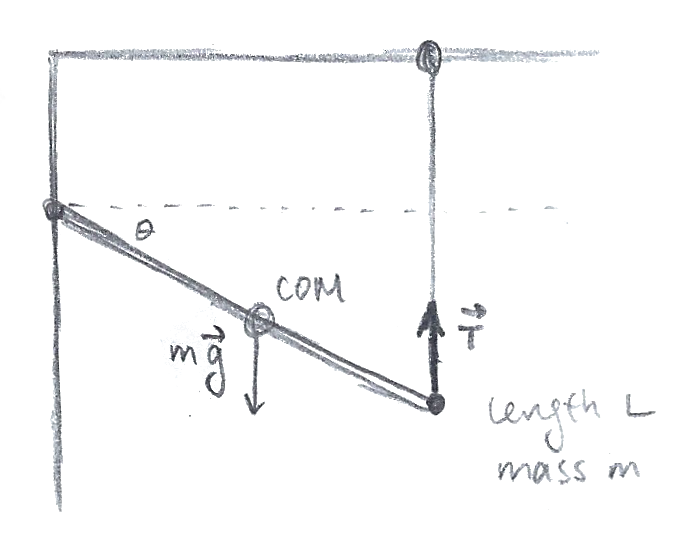
\includegraphics[width=0.4\textwidth]{images/mechintro/statics.png}\\
\end{center}
At first, it seems tempting to just apply Newton's Second Law for all the contact forces and gravity, but quickly it becomes clear that we don't really know how the force from the pivot point really works, and we're missing this information to solve the problem. It's actually much easier to consider the sum of the torques about the pivot point. Since the center of mass of the beam is at the halfway point, the torque due to gravity has magnitude $\tau_g = \frac{L}{2}Mg\cos \theta$. (Make sure you understand why it's cosine and not sine - it's because of the angle between the vectors.) The forces all lie in the same plane, so all the torques run in and out of the page. If we consider up to be the $+y$-direction, right to be the $+x$-direction, and out of the page to be the $+z$-direction (since $\hat x \times \hat y = \hat z$), we have: 
\[
	\sum \tau_z = -\frac{MgL\cos \theta}{2} + \tau_{string} = 0
\]
Therefore, we have that the torque from the string (in the $z$-direction is $\tau_{string} = \frac{MgL\cos \theta}{2}$, since no net torque acts on the system. Noting that $\tau_{string} = TL\cos \theta$, where $T$ is the tension, from this, we can see that the tension $T = \frac{Mg}{2}$. \\
Frequently, aside from using kinematics to look at the system, sometimes we are given that some object or another is rolling without slipping. This means that the following two are true, for a circular object of radius $R$: 
\[
	v_{cm} = \omega R \quad a_{cm} = \alpha R
\]
\begin{center}
	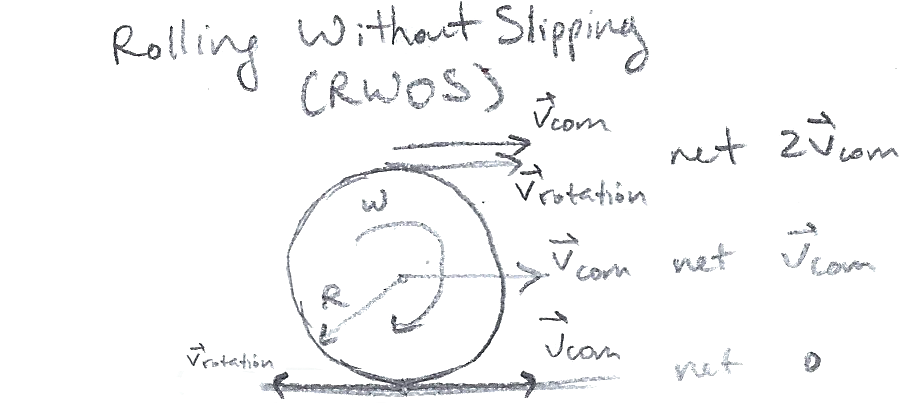
\includegraphics[width=0.4\textwidth]{images/mechintro/rwos.png}\\
\end{center}
When this is true, the frictional force that the object encounters with the ground is actually static and does not change the acceleration of the object. If the object's velocity/angular velocity, etc. do not satisfy these relations, the force of friction will either speed up or slow down the object in order for these two to match so the object starts to roll without slipping. You can see this the next time you go bowling - when you release the ball, the ball slides with constant velocity, but friction begins to turn the ball and it begins to spin faster, and eventually roll normally as the ball travels down the alley. \\
A consequence of the above relations is that relative to the ground, the point in contact with the ground has zero velocity relative to the ground, and the top of the object has speed $2v_{cm}$ relative to the ground. This is very useful to know sometimes - and it can be shown using the principles of relative motion that we discussed in kinematics. \\
Let's revisit Atwood's machine to see how rolling without slipping affects the situation. Consider two masses of $m_1$ and $m_2$ both attached to a taut string ($m_2 > m_1$), wrapped around a solid cylindrical pulley of mass $m_p$ and radius $R$ that is free to spin about its axis. The string does not slip on the pulley, and is still effectively massless. \\
\begin{center}
	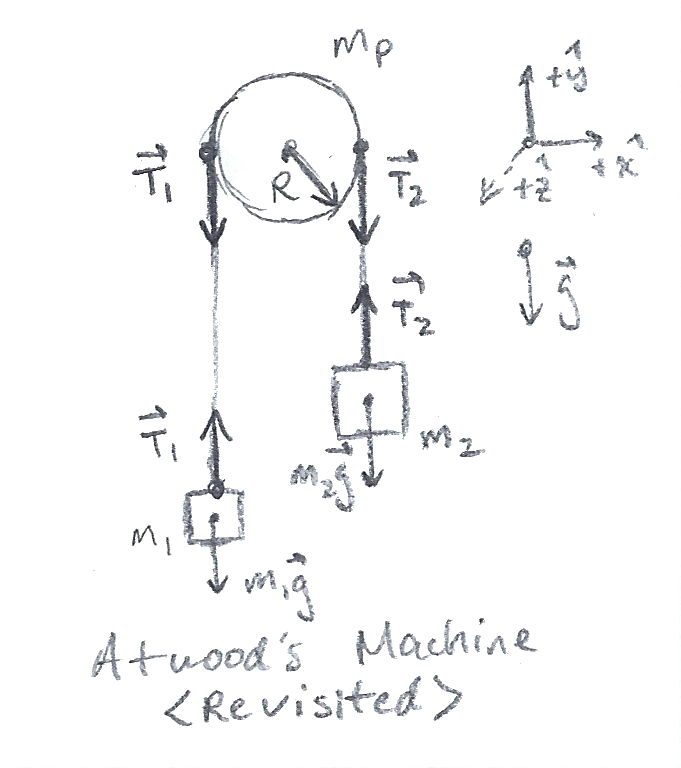
\includegraphics[width=0.4\textwidth]{images/mechintro/atwood-revisited.png}\\
\end{center}
We've drawn an extended free-body diagram to show where each force acts in relation to the objects in the diagram. Notice that the tensions in the strings connecting $m_1$ and $m_2$ to the pulley are not the same, because they're connected to a rotating body now. To distinguish them, let's label the tension on $m_1$ as $T_1$ and the tension on $m_2$ as $T_2$. Let's set up Newton's Second Law, taking into account the force on each of the blocks as well as the torque on the pulley:
\[
	\sum_1 \vec F_i = m_1 \vec g + \vec T_1 = m_1 \vec a
\]
\[
	\sum_2 \vec F_i = m_2 \vec g + \vec T_2 = -m_2 \vec a
\]
\[
	\sum_p \vec \tau_i = \vec R \times \vec T_1 + \vec R \times \vec T_2 = I \vec \alpha
\]
We can project the components of the force in the $+y$-direction (up and down the page), and project the components of the torque along the $+z$-direction (in and out of the page), to get:
\[
	\sum_1 F_y = -m_1g + T_1 = m_1a 
\]
\[
	\sum_2 F_y = -m_2g + T_2 = -m_2a
\]
\[
	\sum_p \tau_z = RT_1 - RT_2 = -I\alpha = -\frac{1}{2}m_pR^2 \alpha
\]
Notice how the sign of the acceleration is reversed for the second block, since we know it's going downwards. Similarly, we've placed a negative sign in front of the angular acceleration since the pulley is rotating clockwise. However, we only have three equations, but we now have four unknowns - the two tensions, the angular acceleration of the pulley, and the acceleration of the blocks. The final thing we need to invoke is the no-slipping condition, which implies the following relation between the angular acceleration of the pulley and the blocks:
\[
	a = R \alpha
\]
We now have all the information we need to solve for the acceleration of the blocks, and the two tensions. Omitting the messy algebra, we have:
\[
	a = \frac{m_2-m_1}{m_1+m_2+\frac{1}{2}m_p}g \quad T_1 = m_1g\frac{4m_2+m_p}{2m_1+2m_2+m_p} \quad T_2 = m_2g\frac{4m_1+m_p}{2m_1+2m_2+m_p} 
\]
Clearly, these expressions are very different than the ones we saw earlier for Atwood's machine, since they now all involve the mass of the pulley from the pulley's moment of inertia.\\
Rolling without slipping problems are a bit more complex, and usually, some information might seem to be missing from the problem in order to solve them. After all, you need to have the same number of variables as equations in order to solve them. If you seem to be missing an equation, it's not a bad idea to impose the rolling without slipping condition on the situation to see if the situation is solvable then. \\
\subsubsection{Summary and Problems}
We now have the tools to look at dynamical systems from a rotational perspective as well as from a translational one. In the following problems, be sure to account for both of these and be able to relate the two different systems of dynamics to each other, with an emphasis on torques, moments of inertia, and angular momentum. \\

\noindent \textbf{Problems}\\
1. (1 $\bigstar$) A uniform cylinder of mass $M$ and radius $R$ has a string wrapped around it. The string is held fixed, and the cylinder falls vertically. a) Show the acceleration of the cylinder is downward with magnitude $a = \frac{2g}{3}$. b) Show the tension in the string $T = \frac{Mg}{3}$. \\
2. (2 $\bigstar$) A uniform solid cylinder of mass $M$ and radius $R$ is at rest on a slab of mass $m$, which in turn rests on a horizontal, frictionless table. If a horizontal force is applied to the slab, it accelerates and the cylinder rolls without slipping. Show the acceleration of the slab is $a = \frac{3F}{3m+M}$.\\
3. (3 $\bigstar$, $\spadesuit$) A uniform horizontal disk of mass $M$ and radius $R$ is spinning about the vertical axis through its center with an angular speed $\omega$. When the spinning disk is dropped onto a horizontal tabletop, kinetic-frictional forces on the disk oppose its spinning motion. Let $\mu_k$ be the coefficient of kinetic friction between the disk and the tabletop. Show that the time required for the disk to stop rotating is $\Delta t = \frac{3R\omega}{4\mu_kg}$. Hint: First, compute the total torque on the disk (from where?) by dividing the disk into thin rings and computing the torque on each ring. \\
4. (2 $\bigstar$) A particle that has a mass $m$ is traveling with a constant velocity along a straight line that is a distance $b$ from the origin $O$. Let $dA$ be the area swept out by the position vector from $O$ to the particle during a time interval $dt$. Show that $\dv{A}{t}$ is constant and is equal to $\frac{L}{2m}$, where $L$ is the magnitude of the angular momentum of the particle about the origin. \\
5. (3 $\bigstar$) A uniform solid sphere with mass $M$ and radius $R$ is set rotating about a horizontal axis at an angular speed $\omega_0$ and then is placed on the floor with its center of mass at rest. If the coefficient of kinetic friction between the sphere and the floor is $\mu_k$ show the speed of the center of mass of the sphere $v = \frac{2R\omega_0}{7}$ when the sphere begins to roll without slipping. \\
6. (4 $\bigstar$) A uniform ladder of length $L$ and mass $m$ leans against a frictionless vertical wall, making an angle of $\theta$ with the horizontal. The coefficient of static friction between the ladder and the ground is $\mu_s$. If your mass is $k$ times that of the ladder, show that the maximum displacement you can move along the ladder $r$ is given by $r = \mu_s L\tan\theta\left(1 + \frac{1}{k}\right) - \frac{L}{2k}$. \\
7. (4 $\bigstar$) A block of mass $M$ rests on a table, connected by a string to a cylindrical (NOT FIXED) pulley of mass $M$ and radius $R$. The string wraps around the pulley and is tied to a block of mass $M$ dangling over the edge of the table. The coefficient of static and kinetic friction between the block on the table and the table is $\frac{1}{2}$. When the system begins moving, the string moves on the cylinder without slipping. Show that the acceleration of each of the blocks is $a = g/5$, and the tensions in the strings are $\frac{4}{5}Mg$ in the string holding the hanging block, and $\frac{7}{10}Mg$ in the string pulling the block along. 
\pagebreak

\subsection{Energy}
The final conserved quantity that we will use to analyze problems is energy. It is the only scalar that we are looking at that is conserved, and is always a positive number. Energy is measured in joules (J), and by definition 1 J = 1 N $\cdot$ m = kg $\cdot$ m$^2$/s$^2$. The rate at which energy is transferred is power and has units of watts (1 W = 1 J/s). 
\subsubsection{Work and Kinetic Energy}
Work is the transfer of energy between objects, and a force is said to do work if the object it is acting upon is displaced, and we might remember it's force times distance - but we need a better definition for work. 
\begin{center}
	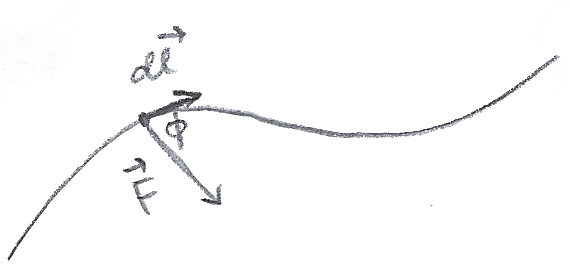
\includegraphics[width=0.3\textwidth]{images/mechintro/work.png}\\
\end{center}
As an object moves along a path while being acted upon by a force, we can split the path into many small displacements. Since work serves to set objects into motion, only the component of the force in the direction of the displacement counts towards the work. So, if the displacement is $d \vec l$, and $\vec F$ is the force, the component of the force in the direction of the displacement is $F \cos \phi$ if $\phi$ is the angle between the displacement and the displacement. This can be written as $\vec F \cdot d\vec l$. Therefore:
\[
	dW = \vec F \cdot d\vec l
\]
where $W$ is the work. For constant force $\vec F$ and linear displacement $d \vec l$ this is true, but to find the total work along any curve $C$, we can let all the little displacements go to zero, let the number of displacements go to infinity and add up all of the little components of work. This is an integral, but a type of integral that we won't encounter in BC Calculus. Somewhat fittingly, this kind of integral is called a line integral, and we can write it as follows:
\[
	W = \int_C \vec F \cdot d\vec l
\]
We won't have to evaluate general line integrals, but for relatively simple cases we will (where the distance is basically linear). \\
This expression for work seems very niche, but we can construct such a line integral from Newton's Second Law, $\vec F = m\vec a = m \dv{\vec v}{t}$. First, we dot the vector on both sides with $\vec v$:
\[
	\vec F \cdot \vec v = m \vec v \cdot \dv{\vec v}{t}
\]
Now, we can integrate with respect to $t$ between times $t_1$ and $t_2$:
\[
	\int_{t_1}^{t_2} \vec F \cdot \vec v \, dt = \int_{t_1}^{t_2} m \vec v \cdot \dv{\vec v}{t} \, dt
\]
The dot product follows the product rule, so I claim that $\frac{1}{2} \dv{}{t}\vec v \cdot \vec v = \vec v \cdot \dv{\vec v}{t}$. Indeed, $\frac{1}{2} \dv{}{t}\vec v \cdot \vec v = \frac{1}{2} \left( \dv{\vec v}{t} \cdot \vec v + \vec v \cdot \dv{\vec v}{t} \right) = \vec v \cdot \dv{\vec v}{t}$. Therefore:
\[
	\int_{t_1}^{t_2} \vec F \cdot \vec v \, dt = \int_{t_1}^{t_2} \frac{1}{2} m \dv{}{t}\vec v \cdot \vec v \, dt = \frac{1}{2} m (\vec v(t_2) \cdot \vec v(t_2) - \vec v(t_1) \cdot \vec v(t_1)) = \frac{1}{2}m (v_{t_2}^2 - v_{t_1}^2 )
\]
The quantity $\frac{1}{2} mv^2$ one might recognize as the kinetic energy $K$ of an object with mass $m$ and velocity $v$, from chemistry. As a refresher, the kinetic energy of an object is the energy the object has that is stored in its movement. This right hand side describes the change in the kinetic energy as the velocity of the object changes during the time interval, so we can write it as $\Delta K$. On the left hand side, since $\dv{\vec l}{t} = \vec v$, $d\vec l = \vec v \, dt$, so we can write the left hand side as an integral along the curve followed by the object during the time interval. In other words, it's our line integral for work! Therefore:
\[
	W = \int_C \vec F \cdot d\vec l = \Delta K
\]
This is the Work-Energy Theorem, which is useful for determining how much work is done to an object after a process by instead measuring its kinetic energy at the beginning and end of the process. \\
As a final sidenote, it's worth noting that kinetic energy has both a translational and rotational form. For an object, a body has translational kinetic energy of $\frac{1}{2}mv^2$, but rotational kinetic energy $\frac{1}{2}I\omega^2$. This expression pops up in the same way when torque is dotted with the angular velocity. Always remember to account for rotational kinetic energy when dealing with rotating objects as well!
\subsubsection{Potential Energy}
Before we introduce the other kind of mechanical energy we'll be studying, potential energy, we have to first introduce the idea of conservative forces versus non-conservative forces. Let's look back at the formula for work: 
\[
	W = \int_C \vec F \cdot d\vec l
\]
For a force $\vec F$, if the work done on the object is independent of the path the object travels, then $\vec F$ is said to be a conservative force. If $\vec F$ does not satisfy this, it is non-conservative. Notice that for $\vec F$ to be conservative, we must have that the work done on an object around a closed loop is zero. Symbolically:
\[
	W = \oint_C \vec F \cdot d\vec l = 0
\]
where the symbol $\oint$ represents integrating around a closed loop (but it's still a line integral). This can be seen by noting that as a particle moves by a conservative force from point $A$ to point $B$, doing some amount of work, the exact negative work is done as the particle moves back from point $B$ to point $A$. With this, we can define the potential energy function $U$ - as work is applied to an object, the potential energy of the object should decrease by the same amount:
\[
	\Delta U = - \int_C \vec F \cdot d\vec l = - W
\]
Usually, potential energy functions are dependent upon the position of the object with respect to the conservative forces at play and give a scalar energy to every point in space, but we'll really only deal with functions in one dimension. The concept is still the same. Also, usually when integrating we'll get a constant - but to simplify things we'll set it to zero, which will sometimes produce negative values of potential energy - but that's fine because it's the relative differences between values that matter more than the actual values. To illustrate this, we'll use an arbitrary one-dimensional conservative force, and look at the potential energy of a particle being acted upon by this force:
\[
	F_x = F_0 \cos \left(\frac{2\pi x}{L} \right)
\]
For the sake of simplicity, both $F_0$ and $L$ have the correct dimensions of force and length, respectively and are both positive.\\ First, let's try to find the potential energy. Consider a path from $x = 0$ to arbitrary $x$ along a straight line. When we do this line integral, then, the dot product basically becomes multiplication, since the force and the displacement are in the same direction, rendering the cosine of the angle between the two to be $1$. Thus, we can calculate $\Delta U$ between these two positions:
\begin{align*}
	\Delta U = U(x) - U_0 &= - \int_C \vec F \cdot d\vec l \\
	&= - \int_0^x  F_0 \cos \left(\frac{2\pi x}{L} \right) \, dx\\
	&= - \frac{F_0L}{2\pi} \sin \left(\frac{2\pi x}{L} \right) \Big|_0^x \\
	&= - \frac{F_0L}{2\pi} \sin \left(\frac{2\pi x}{L} \right)
\end{align*}
If $U_0$ is assumed to be $0$, we can get the not-so-bad-looking function:
\[
	U(x) = - \frac{F_0L}{2\pi} \sin \left(\frac{2\pi x}{L} \right)
\]
This is on the more complex side of potential energy functions we'll be dealing with on a regular basis. The most common ones are the potential energies due to gravity and elastic forces (springs). For these, I'll include them here for you to re-derive. (Note: I'm using $\Delta y$ as a change in the vertical height of an object above the surface of the earth.)
\[
	\vec F = -mg\hat y \quad \Delta U_{grav} = mg\Delta y
\]
\[
	\vec F = -k\Delta x \hat x \quad \Delta U_{spring} = \frac{1}{2}kx^2
\]
\subsubsection{Conservation of Energy}
The fundamental law of the universe is the conservation of mechanical energy $E_{mech}$. We define the mechanical energy of a system $E_{mech}$ to be the sum of the kinetic energy of the system and the potential energy due to all the conservative forces:
\[
	E_{mech} = K_{sys, c} + K_{sys, nc} + U_{sys}
\]
From this, we can observe the following:
\begin{mdframed}[frametitle=Conservation of Mechanical Energy]
If no non-conservative forces act internally in the system, and no external forces put any work into the system, the mechanical energy $E_{mech}$ is constant, and: $$\Delta E_{mech} = \Delta K_{sys} + \Delta U_{sys} = 0$$
More generally, for the universe as a whole, energy cannot be created or destroyed - only converted into other forms.
\end{mdframed}
Notice that if non-conservative forces do act, usually they dissipate energy from the system in the form of heat, a notable example being kinetic friction (static friction does no work). \\
With this in mind, let's revisit the potential energy function that we created in the previous section:
\[
	U(x) = - \frac{F_0L}{2\pi} \sin \left(\frac{2\pi x}{L} \right)
\]
Now, let's launch a particle of mass $m$ from a position with coordinate $x_0$ ($0 < x_0 < \frac{L}{2}$, for simplicity) under the influence of this force. Let's figure out what the maximum velocity of this object is. \\
Intuitively, this can be difficult to imagine. One way we can make this easier for ourselves is to draw an energy diagram. First, we should draw the graph of the potential energy function. In our case, it looks like this:\\
\begin{center}
	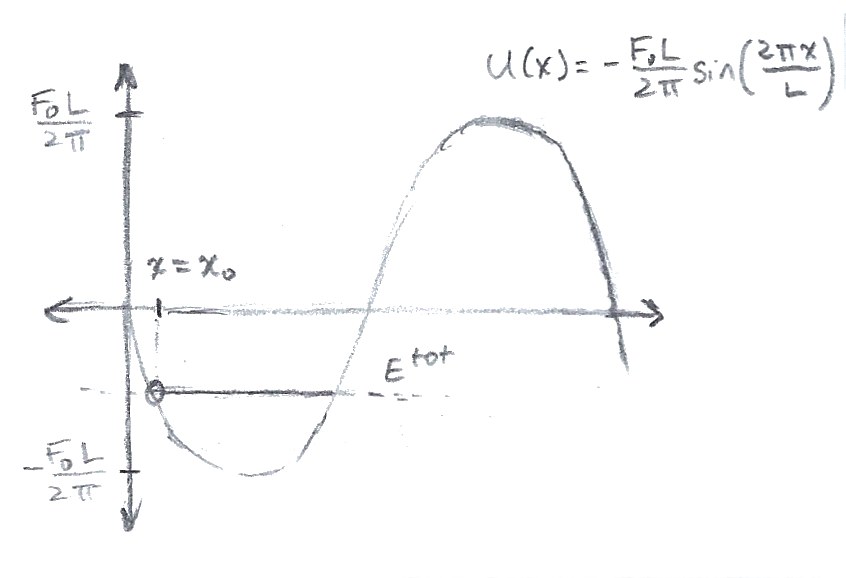
\includegraphics[width=0.5\textwidth]{images/mechintro/cons-energy-1.png}\\
\end{center}
Since there are no external forces on the system and the force is conservative, the energy in the system is conserved. On the graph, we can draw a horizontal line to show how much energy is in the system, as shown. Note that the particle can't reach any position that must cross above the line since otherwise, the system would have more energy than is actually in the system. Therefore, the motion of the particle is restricted to the interval that is bounded by the horizontal line and the potential energy curve. \\
Since potential energy can only be converted to kinetic energy (and vice versa), the particle has its maximum amount of kinetic energy when it has the least amount of potential energy. We can use calculus (or just know how sine functions work, to be honest) to conclude that minimum occurs at $x = \frac{L}{4}$. The potential energy at this point is then:
\[
	U\left(\frac{L}{4}\right) = - \frac{F_0L}{2\pi} \sin \left(\frac{2\pi L}{4L} \right) = - \frac{F_0L}{2\pi}
\]
The change in the potential energy is then:
\[
	\Delta U = U\left(\frac{L}{4}\right) - U(x_0)= \frac{F_0L}{2\pi} \sin \left(\frac{2\pi x_0}{L} \right) - \frac{F_0L}{2\pi}
\]
By conservation of energy, we have $- \Delta U = \Delta K$, so the change in kinetic energy $\Delta K$ is:
\[
	\Delta K = \frac{F_0L}{2\pi}\left(1 - \sin \left(\frac{2\pi x_0}{L} \right)\right)= \frac{1}{2}mv_{max}^2
\]
From this, we get the (pretty messy) expression for the maximum velocity of the particle:
\[
	v_{max} = \sqrt{\frac{F_0L}{\pi m}\left(1 - \sin \left(\frac{2\pi x_0}{L} \right)\right)}
\]
If we launch the particle at some velocity $v_0$, the total energy is higher, because the particle has its own kinetic energy to be accounted for. Let's find the minimum value of $v_0$ for the particle to never return. 
\begin{center}
	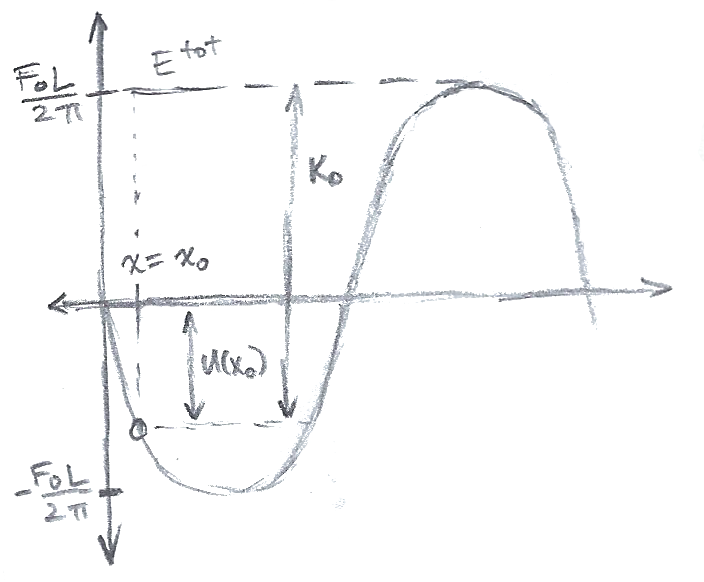
\includegraphics[width=0.4\textwidth]{images/mechintro/cons-energy-2.png}\\
\end{center}
If enough kinetic energy is given to the particle so that it escapes and never comes back to the starting point, the total energy should then be greater than or equal to the maximum value of the potential energy. This means:
\[
	\frac{1}{2}mv_0^2 - \frac{F_0L}{2\pi} \sin \left(\frac{2\pi x_0}{L} \right) = \frac{F_0L}{2\pi}
\]
We can solve and obtain the following expression for $v_0$:
\[
	v_0 = \sqrt{\frac{F_0L}{\pi m} \left(1 + \sin \left(\frac{2\pi x_0}{L} \right) \right)}
\]
The same principles of conservation of energy can be applied to general mechanical systems of a wide variety, as will be seen in the problems.  
\subsubsection{Summary and Problems}
The conservation of energy is a useful principle that can be applied widely to many problems where other dynamical information may not be available. In particular, it tends to provide a helpful link between velocity and position that is not readily attainable from momentum, dynamics, or kinematics. These problems may integrate concepts from all the other units as well - including collisions, which can be classified as elastic, completely inelastic, or partially inelastic. Elastic collisions conserve kinetic energy of the objects before and after the collision, completely inelastic collisions occur when the objects have the same velocity, and partially inelastic collisions satisfy neither of these conditions. Most problems that we will see will either concern a completely inelastic or elastic collision. As a final general rule of thum, remember that if energy is not conserved during a process, be sure to note where that energy goes, whether if it's lost to nonconservative forces such as friction or in a collision. \\

\noindent \textbf{Problems:}\\
1. (2 $\bigstar$) A box slides from rest down a frictionless ramp inclined at an angle $\theta$ with respect to the horizontal and is stopped at the bottom of the ramp by a spring with a spring constant of $k$. If the box has a mass of $m$ and slides a distance $d$ from the point of release to the point where it comes to rest against the spring, show the compression $x$ of the spring when the box comes to rest is $x = \sqrt{\frac{2mgd\sin\theta}{k}}$.\\
2. (3 $\bigstar$) A child of mass $m$ on a playground swing moves with a speed of $v_0$ when the swing of length $L$ is at its lowest point. Show that the angle $\theta$ that the swing makes with the vertical when the child is at the highest point is equal to $\theta = \arccos\left(1- \frac{v_0^2}{2gL}\right)$.\\
3. (3 $\bigstar$) A pendulum consists of a small bob of mass m attached to a string of length $L$. The bob is held to the side with the string horizontal. Then the bob is released from rest. At the lowest point of the swing, the string catches on a thin peg a distance $R$ above the lowest point. Show that $R$ must be smaller than $2L/5$ if the string is to remain taut as the bob swings around the peg in a full circle. \\
4. (2 $\bigstar$)  A small object of mass $m$ moves in a horizontal circle of radius $r$ on a rough table. It is attached to a horizontal string fixed at the center of the circle. The speed of the object is initially $v_0$. After completing one full trip around the circle, the speed of the object is $0.5v_0$. a) Show that the energy dissipated by friction during that one revolution is $\frac{3}{8}mv_0^2$. b) Show that the coefficient of kinetic friction is $\frac{3v_0^2}{16\pi gr}$. c) Show that the object will make a further $\frac{1}{3}$ of a revolution before coming to rest.\\
5. (3 $\bigstar$, $\spadesuit$) The potential energy of a diatomic molecule is given by the following expression with $r$ being the separation of the two atoms of the molecule and $A$ and $B$ being positive constants: $$U = A/r^{12} - B/r^6$$ This potential energy is associated with the force that binds the two atoms together. Show that the equilibrium distance $r$ where no net force acts on either molecule is $1.12(A/B)^{1/6}$.\\
6. (4 $\bigstar$) A pendulum consists of a compact 0.60 kg bob attached to a string of length 1.00 m. A block of mass $m$ rests on a horizontal frictionless surface. The pendulum is released from rest at an angle of 53$^\circ$ with the vertical. The bob collides elastically with the block at the lowest point in its arc. Following the collision, the maximum angle of the pendulum with the vertical is 5.73$^\circ$. Show that the mass $m$ can be equal to both 0.751 kg and 0.479 kg. \\
7. (3 $\bigstar$) A neutron of mass $m$ makes an elastic head-on collision with a stationary nucleus of mass $M$. a) Show that the kinetic energy of the nucleus after the collision is given by $K_{nucleus} = \frac{4Mm}{(m+M)^2}K_n$ where $K_n$ is the initial kinetic energy of the neutron. b) Show that the fractional change in the kinetic energy of the neutron is given by $\frac{\Delta K_n}{K_n} = -\frac{4(m/M)}{1+(m/M)^2}$.
\pagebreak

\subsection{Universal Gravitation}
The last section on mechanics will deal with gravity, starting with Newton's law of Universal Gravitation and looking at why this is consistent with Kepler's Laws of Planetary Motion.
\subsubsection{Newton's Law of Universal Gravitation}
From empirical observations, Newton posited the inverse-square law for gravity, where he claimed the force of gravity between two objects varied as the reciprocal of the square of the distance between the two.\\
\begin{center}
    \begin{asy}
        import geometry;
        size(8cm);
        
        draw(unitcircle);
        draw(shift(15, 0) * unitcircle);
        
        draw((0, -1.5)--(15, -1.5), linetype("8 8"), Arrows);
        draw((1,0)--(3,0), Arrow);
        draw((14,0)--(12,0), Arrow);
        
        label("$m_1$", (0, 1), N);
        label("$m_2$", (15, 1), N);
        label("$r_{12}$", (0, -1.5)--(15, -1.5), S);
        label("$\vec F_{12}$", (1,0)--(3,0), N);
        label("$\vec F_{21}$", (14,0)--(12,0), N);
    \end{asy}
\end{center}
Symbolically, if $m_1$ and $m_2$ are the masses of the two objects, $r_{12}$ is the distance between the two, and $\hat r_{12}$ is the unit vector in the direction from mass 1 to mass 2, then the gravitational force $\vec F_{21}$ on mass 2 due to mass 1 is:
\[
	\vec F = - \frac{Gm_1m_2}{r_{12}^2} \hat r_{12}
\]
The capital $G$ is not the acceleration due to gravity but is the universal gravitational constant that has the weird value of 6.674 $\cdot$ 10$^{-11}$ N$\cdot$m$^2$/kg$^2$. Notice that this formula also holds if you swap masses 1 and 2 - if we define $\hat r_{21}$ as the unit vector from mass 2 to mass 1 instead, so that $\hat r_{21} = - \hat r_{12}$, this still holds. As expected, the negative sign in front of the fraction is to ensure that this is an attractive force, since from real life we can clearly see that gravity pulls things together. 
\subsubsection{Gravitational Fields and Potential Energy}
Moving forward, we're going to work with different kinds of fields. Before moving on, I want to be clear as to what a field is - it's the assignment of some value to every point in space. Mostly, we're going to look at vector fields and scalar fields - fields where a vector/scalar are assigned to every point. The first ones we'll encounter in physics are the gravitational field and the gravitational potential. \\
Consider placing a very small test point particle $m_0$ amongst a collection of masses. These masses exert a gravitational force $\vec F_{net}$ on the particle:
\[
	\vec F_{net} = \sum_i \vec F_i = \sum_i -\frac{Gm_0m_i}{r_i^2}\hat r_i
\]
(For clarity - I'm using $m_i$ as the mass of the $i$th particle, $r_i$ for the distance between $m_0$ and $m_i$, and $\hat r_i$ as the unit vector in the direction from $m_0$ to $m_i$.)\\
Now, define the gravitational field at the position of the test mass $m_0$ as the net gravitational force divided by the mass of the small test particle:
\[
	\vec g = \frac{\vec F_{net}}{m_0} = \sum_i -\frac{Gm_i}{r_i^2}\hat r_i
\]
Notice for a single point mass, then, we have the gravitational field $\vec g = -\frac{Gm_i}{r^2}\hat r$ where $r$ is the distance from the point mass and $\hat r$ is just radially outward from the mass. However, more likely than not we are going to encounter continuous distributions of mass, which will require integration and superposing infinitely many small gravitational fields to create the total field. Here, we're going to derive the gravitational field due to a thin ring of mass and for a spherical shell. \\
\begin{center}
    \begin{asy}
        import three;
        size(6cm);
        triple eye = (7, 8, 5);
        currentprojection = perspective(eye);
        triple center = (0, 0, 0);
        real R = 1, y = 2;
        draw(circle(center, R, Z));
        dot((0, 0, y));
        real dqAngle = -20, dqDelta = 6;
        draw(arc(center, R,
                90, dqAngle - dqDelta,
                90, dqAngle + dqDelta), linewidth(2));
        draw(dir(90, dqAngle) -- (0, 0, y), linetype("6 6"));
        triple radiusPt = R * dir(90, 170);
        draw((0, 0, 0)--radiusPt, gray(0.2));
        draw((0, 0, 0)--(0, 0, y), gray(0.2));
        
        label("$M$", (0, R, 0), dir(-90));
        label("$m_0$", (0, 0, y), dir(130));
        label("$dM$", dir(90, dqAngle), dir(200));
        label("$R$", radiusPt/2, dir(-40));
        label("$y$", (0, 0, y/2), dir(0));
    \end{asy}
\end{center}
First, let's consider a uniform ring of mass $M$ and radius $R$, and for simplicity let's use a test mass $m_0$ on the axis of symmetry of the ring, at a distance of $y$ above the center. This ring has a linear mass density $\lambda = \frac{M}{2\pi R}$. We can consider dividing the ring into infinitely many tiny arcs, with length $ds = R \, d\theta$. The mass of this piece can then be shown to be $dm = \lambda R \, d\theta$. \\
From this, we conclude the magnitude of the force on the test mass from this small arc, $dF$, is
\[
    dF = \frac{Gm_0 \,dm}{R^2 + y^2}
\]
Note that the radial components of the force will cancel each other out by symmetry, so it suffices to consider the components of the force in the $y$-direction, $dF_y$:
\[
    dF_y = -\frac{Gm_0 \, dm}{R^2 + y^2} \cdot \frac{y}{\sqrt{R^2+y^2}} = \frac{Gm_0 \, dm \, y}{(R^2 + y^2)^{3/2}}.
\]
The negative sign is present since gravity is an attractive force. We can now integrate over all the small bits of mass: 
\begin{align*}
    F &= \int_0^{2\pi} dF_y \\
    &= \int_0^{2\pi} -\frac{Gm_0 \, dm \, y}{(R^2 + y^2)^{3/2}} \\
    &= \int_0^{2\pi} -\frac{Gm_0y \lambda R \, d \theta}{(R^2 + y^2)^{3/2}}\\
    &= -\frac{Gm_0My}{(R^2 + y^2)^{3/2}}.
\end{align*}
The force is directed in the negative $y$-direction, and thus the force is
\[
    \vec F = -\frac{Gm_0My}{(R^2 + y^2)^{3/2}}\hat y
\]
To find the gravitational field along the axis at any distance from the center $y$, we simply use our definition to find:
\[
    \vec g = \frac{GMy}{(R^2 + y^2)^{3/2}}\hat y.
\]
\begin{center}
    \begin{asy}
        import solids;
        import three;
        size(8cm);
        
        currentprojection=orthographic(0.7, -4, 1);
        currentlight=nolight;
        triple center = (0,0,0);
        triple ringctr = (0.5, 0, 0);
        real R=1, RS=0.7, inc=100, lat=45, lon=45, tlat=50, tlon=100;
        dot(center);
        real r = 2;
        dot(ringctr);
        revolution Earth=sphere(center, R);  
        
        draw(surface(Earth), surfacepen=white+opacity(.1), meshpen=0.7*black);
        draw(arc(ringctr, sqrt(3)/2, 0, 90, 180, 270), linewidth(2));
        draw(arc(ringctr, sqrt(3)/2, 180, 270, 0, 90), linewidth(2)+linetype("4 4"));
        dot((r, 0, 0));

        draw((0,0,0)--(r, 0, 0));
        draw(center--(0.5, 0, sqrt(3)/2));
        label("$R$", (0.25, 0, sqrt(3)/4), dir(120));
        label("$dM$", (0.5, 0, sqrt(3)/2), dir(40)*1.5);
        label("$\theta$", center, dir(30)*2);
        label("$r$", (r*0.75, 0, 0), dir(90));
        label("$m_0$", (r, 0, 0), dir(50));
    \end{asy}
\end{center}
From here, we can proceed to find the gravitational field of a uniform thin spherical shell of mass $M$ and radius $R$, making the surface density $\sigma = \frac{M}{4\pi R^2}$. Consider a test mass $m_0$, a distance $r$ away from the center of the sphere. We can split the sphere into many rings and use a scanning variable $\theta$ that represents the angle between the line joining the center to the edge of the ring and the horizontal. The surface area of each ring $dA = 2\pi R^2 \sin \theta \, d\theta$ (as seen before in the moment of inertia calculation), so then mass of each ring, $dm$, can be seen to be $dm = 2\pi \sigma R^2 \sin \theta \, d\theta$. We can then plug straight back into the formula for a ring to get: 
\[
    dF = \frac{Gm_0(r-R\cos \theta)\, dm}{((R\sin \theta)^2 + (r-R\cos \theta)^2)^{3/2}} = \frac{2Gm_0R^2 \pi \sigma (r-R\cos \theta) \sin \theta \, d\theta}{((R\sin \theta)^2 + (r-R\cos \theta)^2)^{3/2}}
\]
We integrate with respect to $\theta$ from $0$ to $\pi$, and simplify as much as possible: 
\begin{align*}
    F &= \int_0^\pi \frac{2Gm_0R^2 \pi \sigma (r-R\cos \theta) \sin \theta \, d\theta}{((R\sin \theta)^2 + (r-R\cos \theta)^2)^{3/2}}\\
    &= Gm_0\pi\sigma \int_0^\pi \frac{2R^2 (r-R\cos \theta) \sin \theta \, d\theta}{(R^2 + r^2 - 2rR\cos \theta)^{3/2}}
\end{align*}
Let $u = R^2 + r^2 - 2rR\cos \theta$, and $du = 2rR \sin \theta \, d\theta$, which changes the bounds to $(r-R)^2$ to $(r+R)^2$. From this, we also get that $\cos \theta = \frac{R^2+r^2-u}{2Rr}$ and gives
\begin{align*}
    F &= Gm_0\pi\sigma \int_{(r-R)^2}^{(r+R)^2} \frac{R}{r} \left(r-\frac{R^2+r^2-u}{2r}\right) u^{-\frac{3}{2}}\, du \\
    &= \frac{Gm_0\pi\sigma R}{2r^2} \int_{(r-R)^2}^{(r+R)^2} (r^2-R^2+u) u^{-\frac{3}{2}}\, du \\
    &= \frac{Gm_0\pi\sigma R}{2r^2} \int_{(r-R)^2}^{(r+R)^2} (r^2-R^2)u^{-\frac{3}{2}} + u^{-\frac{1}{2}}\, du \\
    &= \frac{Gm_0\pi\sigma R}{2r^2} (-2(r^2-R^2)u^{-\frac{1}{2}} + 2u^{\frac{1}{2}}) \Big|_{(r-R)^2}^{(r+R)^2} \\
    &= \frac{Gm_0\pi\sigma R}{r^2} ((R^2-r^2)u^{-\frac{1}{2}} + u^{\frac{1}{2}}) \Big|_{(r-R)^2}^{(r+R)^2}\\
\end{align*}
\textbf{Case 1: Outside the Shell} \newline
Assume now that $r > R$, so $r - R> 0$. Evaluating, we have
\begin{align*}
    F &= \frac{Gm_0\pi\sigma R}{r^2} \left(\frac{R^2-r^2}{r+R} + R+r - \frac{R^2-r^2}{r-R} - (r - R)\right) \\
    &= \frac{Gm_0\pi\sigma R}{r^2} (R-r + R+r + R+ r + R -r)\\
    &= \frac{Gm_0\pi\sigma 4R^2}{r^2} \\
    &= \frac{Gm_0Q}{r^2} 
\end{align*}
From this, we see that 
\[
    \vec g = \frac{GM}{r^2}\hat r
\]
where $\hat r$ is the unit vector radially outward from the center of the sphere to the point charge. \\ 
\textbf{Case 2: Inside the Shell} \\
Assume now that $r < R$, so $R - r> 0$. Evaluating, we have
\begin{align*}
    F &= \frac{Gm_0\pi\sigma R}{r^2} \left(\frac{R^2-r^2}{r+R} + R+r - \frac{R^2-r^2}{R-r} - (R-r)\right) \\
    &= \frac{Gm_0\pi\sigma R}{r^2} (R-r + R+r - R - r -R + r)\\
    &= 0
\end{align*}
and clearly $\vec g = 0$. Notice that outside the shell, the field is exactly the same as if the shell was essentially a point mass, and on the inside, it's zero. This is a result known as the Shell Theorem. \\
Another field that we will investigate is a scalar field, the potential energy field. First, let's look at the gravitational potential energy of a mass $m_0$ brought from arbitrarily far away (so, basically infinity) to a distance $r$ away from a mass $M$. Assuming the potential energy at infinity is zero, the potential energy function $U(r)$ is then:
\[
	U = - \int_r^{\infty} F \, dr = - \int_r^{\infty} -\frac{Gm_0M}{r^2} \, dr = -\frac{Gm_0M}{r}
\]
This also follows the principles of superposition that is true for gravitational fields, but direction need not be taken into account because energy is a scalar. For reference, here are the potential energies of a test particle $m_0$ near the ring and shell:
\[
	U = -\frac{GMm_0}{\sqrt{R^2 + y^2}} \quad U = -\frac{Gm_0M}{r}
\]
\subsubsection{Kepler's Laws of Planetary Motion}
Before Newton, Kepler proposed three laws of planetary motion from empirical data of the positions of astronomical bodies as they orbited the sun. These are the laws Kepler proposed: \\
1. All planets orbit around a sun in elliptical orbits with the sun at one focus of the ellipse.\\
2. Planets sweep out equal-sized areas in equal time intervals. \\
3. The square of the period of a planet's orbit is proportional to the cube of the semi-major axis of the planet's orbit: more specifically, 
\[
	T^2 = \frac{4\pi^2}{GM} a^3
\]
where $M$ is the mass of the sun. \\
% \section*{Appendix A: Proof of Kepler's Laws}
% \addcontentsline{toc}{section}{Appendix A: Proof of Kepler's Laws}
% As a reminder, here is a restatement of Kepler's Laws:\\
% 1. All planets orbit around a sun in elliptical orbits with the sun at one focus of the ellipse.\\
% 2. Planets sweep out equal-sized areas in equal time intervals. \\
% 3. The square of the period of a planet's orbit around a mass $M$ is proportional to the cube of the semi-major axis of the planet's orbit: more specifically, 
% \[
% 	T^2 = \frac{4\pi^2}{GM} a^3
% \]
The first and third statements follow from Newton's Law of Universal Gravitation, but the second is essentially a disguised conservation of angular momentum (see the problems from Rotation!). We're going to prove these two using Newton's Law of Universal Gravitation and Newton's Second Law of Motion. \\
\begin{center}
	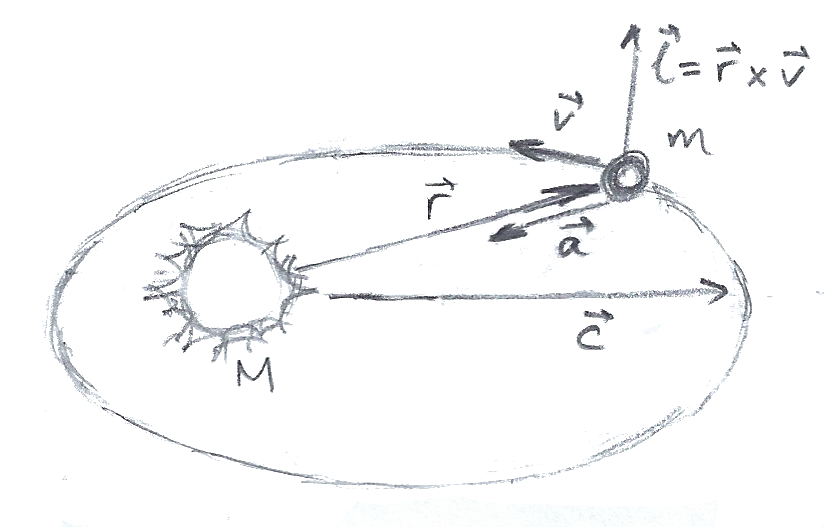
\includegraphics[width=0.5\textwidth]{images/mechintro/kepler-1.png}\\
\end{center}
If a satellite of mass $m$ is orbiting around a mass $M$, the force $\vec F = - \frac{GmM}{r^2} \hat r$ where $\hat r$ and $r$ are varying with time. Because of this, notice that $\vec a =  - \frac{GM}{r^2} \hat r$ from Newton's Second Law. The position $\vec r$ and $\vec a$ are then always in the same direction. \\
Assuming no other forces act on the system, the orbital angular momentum $\vec L = \vec r \times m \vec v$ is constant. We're more interested in the fact that the cross product $\vec r \times \vec v$ is also a constant, so we're going to denote this by $\vec l$. But what exactly is $\vec l$? We can do this explicitly:
\begin{align*}
	\vec l &= \vec r \times \vec v \\
	&= \vec r \times \dv{\vec r}{t}\\
	&= r \hat r \times \dv{}{t}(r \hat r)\\
	&= r \hat r \times (r' \hat r + r \hat r')\\
	&= r^2(\hat r \times \hat r')\\
\end{align*}
We're going to do something a little contrived: what happens when we take $\vec a \times \vec l$? We can use the triple vector product identity to help us out, and the fact that we've decomposed everything into unit vectors with magnitude 1:
\begin{align*}
	\vec a \times \vec l &=  - \frac{GM}{r^2} \hat r \times r^2 (\hat r \times \hat r')\\
	&= -GM [ \hat r (\hat r \cdot \hat r') - \hat r' (\hat r \cdot \hat r) ]\\
	&= GM \hat r'
\end{align*}
The first dot product in parentheses is zero - the derivative of a unit vector is always perpendicular to the original. If you're not convinced, look at $\hat r$ and $\hat \theta$ when we derived circular motion - $\hat \theta$ is proportional to the derivative of $\hat r$, and $\hat \theta \cdot \hat r = 0$. \\
Since we know how $\vec a \times \vec l$, we can find $\vec v \times \vec l$. Considering that 
\[
	\dv{}{t} (\vec v \times \vec l) = \dv {\vec v}{t} \times l + \vec v \times \dv{\vec l}{t} = \vec a \times \vec l + \vec v \times \vec 0 = \vec a \times \vec l
\]
we can integrate to find $\vec v \times \vec l = GM \hat r + \vec c$ for some constant vector $\vec c$. \\
We have one more contrived step to take: consider $\vec r \cdot (\vec v \times \vec l)$. We can expand it as follows:
\begin{align*}
	\vec r \cdot (\vec v \times \vec l) &= \vec r \cdot (GM \hat r + \vec c) \\
	&= GM (\vec r \cdot \hat r) + \vec r \cdot \hat c\\
	&= GMr + rc \cos \theta
\end{align*}
where $\theta$ is the angle between $\vec r$ and $\vec c$. On the other hand, since this is a scalar triple product, $\vec r \cdot (\vec v \times \vec l) = \vec l \cdot (\vec r \times \vec v) = \vec l \cdot \vec l = l^2$. Therefore, 
\[
	l^2 = GMr + rc \cos \theta
\]
\[
	r = \frac{l^2}{GM + c \cos \theta} = \frac{\frac{l^2}{GM}}{1 + \frac{c}{GM} \cos \theta}
\]
That is the polar equation for an ellipse, centered at one of its foci (if you might recall from the conics unit), and this gives Kepler's First Law.\\
\begin{center}
	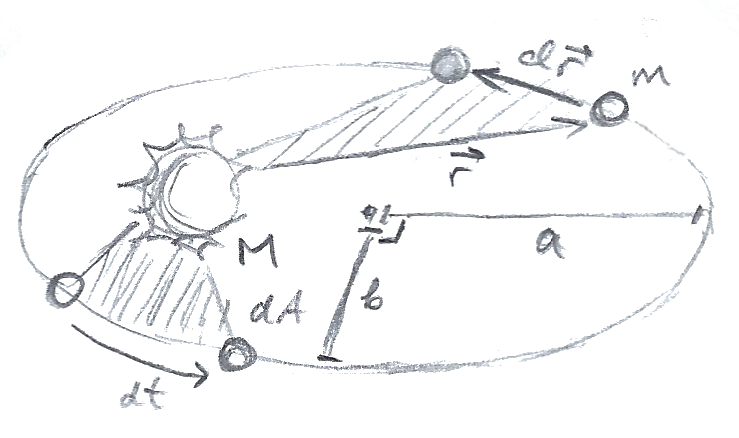
\includegraphics[width=0.5\textwidth]{images/mechintro/kepler-2.png}\\
\end{center}
For Kepler's Second Law, we reuse the fact that $\vec l = \vec r \times \vec v$ is a constant. Consider a small triangular area $dA$ swept out in a time $dt$ by a satellite. This area $dA = \frac{1}{2}| \vec r \times d\vec r |$, where $d\vec r$ is the displacement of the satellite. Dividing by $dt$ gives $\dv{A}{t} = \frac{1}{2} \left| \vec r \times \dv{\vec r}{t} \right| = \frac{1}{2} \left| \vec r \times \vec v \right| = \frac{1}{2} l$. Since $\vec l$ is constant, we have that the area swept out per unit time is constant, so the area swept out by a satellite in a given time interval is also a constant. \\
Using this, we can prove Kepler's Third Law. The rate at which area is swept out is $\dv{A}{t} = \frac{1}{2} l$ by Kepler's Second Law, but since this is constant it's also equal to the total area of the elliptical orbit over the period of the motion. Letting $a$ and $b$ be the lengths of the semi-major and semi-minor axes, we have 
\[
	\dv{A}{t} = \frac{\pi a b}{T} = \frac{1}{2}l
\]
From this, we see that 
\[
	T = \frac{2\pi a b}{l} \rightarrow T^2 = \frac{4\pi^2 a^2 b^2}{l^2}
\]
I'm going to gloss over this part a little bit - but recall that an ellipse in polar coordinates is defined by its eccentricity $e$ and the distance from the focus to the directrix $d$. The computation is extremely messy, but it can be shown (with great effort) that the numerator of the polar equation $ed = \frac{b^2}{a}$. In this case, then, $\frac{l^2}{GM} = \frac{b^2}{a}$, which is equivalent to $\frac{b^2}{l^2} = \frac{a}{GM}$. We can plug this back in to get
\[
	T^2 = \frac{4\pi^2}{GM}a^3
\]
This shows Kepler's Third Law. Usually, however, we won't work with actual elliptical orbits - most of the time we will just deal with simplified circular orbits, where the semi-major axis is just the radius of the circle. 
These equations hold true in general for satellites orbiting around large masses, if the satellite's mass is negligible - otherwise, one must consider orbit around the center of mass and use the total mass for Kepler's Third Law. We will see why this is as a problem at the end of the chapter.
\subsubsection{Summary and Problems} 
Using Newton's Law of Gravitation and our knowledge of mechanics up to this point, we derived Kepler's Laws and we can now apply them in these problems. As a result of Newton's Law of Gravitation, we were also able to derive a gravitational field which we will calculate for a few setups. We can also look at the potential energy of gravitational fields, which we will also explore a little. \\

\noindent\textbf{Problems:}\\
1. (1 $\bigstar$) Given that the mean period of the Moon's orbit is 27.3 days, the mean orbital radius of the Moon around the Earth is 385,000 km, and the value of $G$, approximate the mass of the Earth to be about 6.07$\cdot$10$^{24}$ kg. \\
2. (2 $\bigstar$, $\spadesuit$) Two particles, each of mass $M$, are fixed in position on the $y$-axis at $y = +a$ and $y = -a$. Show that on the $x-$axis, the maximum value of $g$ for the gravitational field occurs at points $x = \pm a/\sqrt{2}$. \\
3. (3 $\bigstar$) An object is projected vertically from the surface of Earth at less than the escape speed. Show that the maximum height $H$ reached by the object is $H = \frac{R_EH'}{R_E - H'}$, where $H'$ is the height that it would reach if the gravitational field were constant, and $R_E$ is the radius of the Earth. Notice that for large values of the launch velocity for a projectile, this model is more precise if significant fluctuations in the gravitational field are observed over the course of the object's flight.\\
4. (4 $\bigstar$, $\spadesuit$) A uniform thin rod of mass $M$ and length $L$ lies on the $+x$-axis with one end at the origin. Consider an element of the rod of length $dx$, and mass $dm$, at point $x$, where $0<x<L$. a) Show that this element produces a gravitational field $dg_{x}$ at a point $x_0$ on the $x-$axis in the region $x_0 > L$ is given by $dg_{x} = -\frac{GM}{L(x_0-x)^2}$. b) Show that the total gravitational field at the point $x_0$ due to the rod is $g = \frac{GM}{x_0(x_0-L)}$. c) Show that for $x_0 >> L$, the field of the rod approximates the field of a point particle of mass $M$ at $x = 0$. d) Using a similar method, compute the gravitational potential energy of a mass $m_0$ at a position $x_0$ to be $U = -\frac{GMm_0}{L} \ln\left(\frac{x_0+L/2}{x_0-L/2}\right)$.\\
5. (3 $\bigstar$) In a binary star system, two stars follow circular orbits about their common center of mass. If the stars have masses $m_1$ and $m_2$ and are separated by a distance $r$, show that the period of rotation is related to $r$ by $T^2 = \frac{4\pi^2}{G(m_1+m_2)}r^3$. \\
6. (2 $\bigstar$) Four identical planets are arranged in a square of side length $a$. If the mass of each planet is $M$, show that the speed of each planet is $v = \sqrt{\frac{GM}{a}\left(\frac{\sqrt{2}}{4} + 1 \right)}$ if they are to orbit their common center under the influence of their mutual attraction.\\
7. (3 $\bigstar$) Two particles of masses $m_1$ and $m_2$ are released from rest at a large separation distance. Show that their speeds $v_1$ and $v_2$ when their separation distance is $r$ are $v_1 = \sqrt{\frac{2Gm_2^2}{r(m_1+m_2)}}$ and $v_2 = \sqrt{\frac{2Gm_1^2}{r(m_1+m_2)}}$.
\pagebreak

\section*{Mechanics Highlights}
\addcontentsline{toc}{section}{\protect\numberline{}Mechanics Highlights}
Some of my personal favorite mechanics problems. These are hard problems, but I strongly encourage you to give most of these a try (except problem 1), because they're good problems. If you feel like you've attempted a problem several times and come up with an incorrect answer, I'd be happy to discuss these with you and go over them. \\
\textbf{Problems:}\\
1. (?? $\bigstar$) Find as many mistakes/inaccuracies as you can find in the Mechanics section. \\
2. (4 $\bigstar$) A solid bowling ball of mass $M$ and radius $R$ has an initial clockwise angular velocity $\omega_0$ down the lane and an initial speed of the the center of mass of the ball $s = \frac{R\omega_0}{3}$ just after its release. The coefficient of kinetic friction is $\mu_k$. Show that the final angular momentum of the ball about its initial point of contact with the floor is $\frac{11}{15}MR^2 \omega_0$.\\
3. (3 $\bigstar$) Consider a solid cylinder that has mass $M$ and radius $R$ to which a second solid cylinder that has mass $m$ and radius $r$ is attached. These cylinders share an axis of symmetry. A string is wound about the smaller cylinder. The larger cylinder rests on a horizontal surface. The coefficient of static friction between the larger cylinder and the surface is $\mu_k$. If a light tension is applied to the string in the vertical direction, the cylinder will roll to the left; if the tension is applied with the string horizontally to the right, the cylinder rolls to the right. Show that the angle between the string and the horizontal that will allow the cylinder to remain stationary when a
light tension is applied to the string is $\theta = \arccos \frac{r}{R}$. \\
4. (3 $\bigstar$) A boy is initially seated on the top of a hemispherical ice mound of radius $R$. He begins to slide down the ice, with a negligible initial speed. Approximate the ice as being frictionless. Show that the height where the boy loses contact with the ice is $\frac{2}{3}R$. \\
5. (4 $\bigstar$, $\spadesuit$) A rod of mass $M$ and length $L$ acts as a solid pendulum. Its pivot point is set a distance $d$ from its center of mass (in the center of the rod). Show that if the rod is set swinging (at small angles) and exhibits simple harmonic motion, the period of the motion can be maximized by setting $d = \frac{L}{2\sqrt{3}}$. Hint: Use blasphemy - $\sin \theta = \theta$ for small values of theta :P. \\
6. (5 $\bigstar$) A long rod of mass $M$ and length $L$ is at rest on a frictionless horizontal surface. A small blob of mass $M$ moving at a speed $s$ strikes the rod at one of its ends, and sticks to the rod. Show that the ratio of the total kinetic energy in the system before the collision to the total kinetic energy after the collision is $\frac{4}{5}$. \\
7. (4 $\bigstar$) A uniform rod with mass $M$ and length $L$ turns without friction on a fixed pivot at the end of the rod. The rod is released from rest from a horizontal position. The rod swings down, collides with a small dense block, also with mass $M$, and the block sticks to the end of the rod. Show that the maximum angular displacement of the rod from the vertical after the collision is $\theta = \arccos\left(\frac{11}{12}\right)$.\\
8. (5 $\bigstar$, $\spadesuit$) Two small blocks with masses $M$ and $2M$ are attached to a spring with negligible mass, spring constant $k$, and natural length $L$. The blocks and spring rest on a frictionless horizontal surface with the lighter block in contact with a wall located at $x=0$. The system is released from rest at time $t=0$ with the spring compressed to a length $\frac{L}{2}$. Show that the maximum length of the spring after the lighter block leaves the wall is $\left(1 + \frac{1}{2\sqrt{3}}\right) L$ and the location of the center of mass of the two-block system when this occurs is $\frac{\pi\sqrt{3}+2}{3}L$.
\pagebreak


\part{Electricity and Magnetism}
The second half of the course is dedicated to studying another fundamental force, that being electromagnetism, and the interactions between the physical world that we already know how to analyze and the carriers of this force, electric charges.  
\section{Electrostatics}
We don't have a good non-circular definition of what exactly electric charge is, but we can certainly measure it. The units of electric charge are called coulombs and denoted with a C. \\
It turns out that electric charge is quantized, meaning that it comes in discrete amounts. Any amount of electric charge comes in integer multiples of the fundamental unit of charge $e$, which is measured to be $e$ = 1.60 $\cdot$ 10$^{-19}$ C. This is a really small number - so small, in fact, that we effectively treat charge as a continuous quantity that can take on any real value. Clearly, this is not true - but the macroscopic quantities of charge that we will work with will basically behave as if charge were continuous. This means that we can use calculus and the math we used in mechanics, even with the knowledge that particles carry strictly integer amounts of the fundamental unit of charge (even if they are very large integers). \\
Charges can be positive, negative, or zero. Regardless of what value we assign to the charge because we will generally be deriving formulas in terms of a variable representing the charge, the math will still turn out the same. Therefore, there isn't really a need to rederive all the formulas that we need for negative charges as well as for positive ones because they should be the same depending on what value we plug in. However, qualitatively, we will just assume charges are positive to get a feel for how the formulas work.\\
Before studying charges in motion, we will first discuss the behaviors and interactions of stationary charges. This study is called electrostatics and is the foundation upon which we will build our knowledge of electromagnetism. 
\subsection{Coulomb's Law}
We first must answer the question: How does charge interact with itself? We already probably know that charges with the same sign repel each other, and charges with differing signs attract, as observed in nature. This force also should decrease in magnitude as the distance between the charges increases - after all, if you move oppositely charged things really far away from each other, there doesn't appear to be an observable force between them, whereas a much more observable one appears once the charges are close enough. A clever scientist by the name of Charles-Augustin de Coulomb came up with his self-named law that describes the electric force between two charges $q_1$ and $q_2$, using macroscopic observations. If $r_{12}$ is the distance between these charges, and the unit vector $\hat r_{12}$ is the unit vector that points from charge $q_1$ in the direction of $q_2$, we have that the force exerted on charge $q_2$ by $q_1$ is:
\[
	\vec F = \frac{kq_1q_2}{r_{12}^2} \hat r_{12}
\]
\begin{center}
    \begin{asy}
        import geometry;
        size(8cm);
        
        draw(unitcircle);
        draw(shift(15, 0) * unitcircle);
        draw((-1,0)--(-3,0), Arrow);
        draw((16,0)--(18,0), Arrow);
        
        draw((0, -1.5)--(15, -1.5), linetype("8 8"), Arrows);
        
        label("$q_1$", (0, 1), N);
        label("$q_2$", (15, 1), N);
        label("$r_{12}$", (0, -1.5)--(15, -1.5), S);
        label("$\vec F_{12}$", (-1,0)--(-3,0), N);
        label("$\vec F_{21}$", (16,0)--(18,0), N);
    \end{asy}
\end{center}
Notice how this is also an inverse-square law, just like the force of gravity - in fact, it's essentially the same, up to a sign and the proportionality constant, $k$. In this case, $k$ is Coulomb's constant, and has been measured to be 8.99 $\cdot$ 10$^9$ N $\cdot$ m$^2$/C$^2$. Sometimes, we will see Coulomb's Law written in the following manner:
\[
	\vec F = \frac{1}{4 \pi \epsilon_0} \frac{q_1q_2}{r_{12}^2} \hat r_{12}
\]
where the $k$ has been replaced with $\frac{1}{4 \pi \epsilon_0}$. These expressions are the same, except now our proportionality constant is written in terms of $\epsilon_0$, called the permeability of free space. This has a value of 8.85 $\cdot$ 10$^{-12}$ C$^2$/(N $\cdot$ m$^2$), and it'll come up often in place of $k$ (for reasons we will discuss later). 
\subsection{Electric Fields and Superposition}
When we introduced the gravitational force, we also introduced the gravitational field, which assigned a vector to every point in space that represented the force done per unit mass. We can do something similar for the electric force. For a charge $q_0$, and a net electric force on this particle $\vec F_{net}$, we have that the electric field at this point $\vec E$ is:
\[
	\vec E = \frac{\vec F}{q_0}
\]
Just like with gravity, we will have to calculate the electric field not just for collections of point charges, but also for continuous distributions of charge. Because of the similarity between the gravitational and electric forces, all of the formulas derived using superposition of forces and fields in the gravity section essentially apply to electrostatics. We can follow the same logic employed there to arrive at the electric field on the axis of a uniform ring of change, and the electric field due to a thin spherical shell of charge:
\[
	\text{Ring: } \vec E = \frac{kQy}{(R^2 + y^2)^{3/2}}\hat y \quad \text{Spherical Shell, outside: } \vec E = \frac{kQ}{r^2}\hat r \quad \text{Spherical Shell, inside: } \vec E = 0
\]
We're going to calculate two more fields here - one being the field due to an infinite line charge, and the other the field of an infinite plane charge. \\
For the infinite line charge, we can assume it's uniform with linear charge density $\lambda$ and we can parameterize it using the real number line. For simplicity, we'll place a test charge $q_0$ radially outward from the line a distance of $y$ away at $x$-coordinate $x=0$.\\
\begin{center}
    \begin{asy}
        import geometry;
        size(9cm);
        
        real y = 5;
        dot((0, y));

        draw((0,0)--(-10,0), linetype("4 4"), Arrow);
        draw((0,0)--(10,0), linetype("4 4"), Arrow);
        draw((-4.25,0)--(0,y), linetype("6 6"));
        draw((0, y)--(0,0));
        draw((-4,0)--(-4.5,0), linewidth(2));

        label("$y$", (0, y/2), dir(0));
        label("$x$", (-2, -0.5), dir(270));
        label("$dx$", (-4.25, -0.5), dir(270)*0.2);
        label("$q_0$", (0, y), dir(130));
    \end{asy}
\end{center}
Consider now an infinitesimal subdivision of the line with length $dx$ and at coordinate $x$. The charge of this point is $dq = \lambda \, dx$, and we can use Coulomb's Law to figure out the force on the test charge:
\[
	dF = \frac{kq_0\, dq}{x^2 + y^2}
\]
This, however, is the magnitude of the force - we haven't taken into consideration that all the components in the $x$-direction will cancel, by symmetry. Therefore, we have to project into the radial direction and find the $r$-component of the force, where the $r$-direction is radially outward from the cylindrical symmetry of the wire. 
\[
	dF_r = \frac{kq_0 \, dq \, y}{(x^2 + y^2)^{3/2}}
\]
The electric field due to the small portion of the wire is then:
\[
	dE_r = \frac{k\lambda y \, dx}{(x^2+y^2)^{3/2}}
\]
We now have to integrate over all these portions of wire, from $-\infty$ to $\infty$:
\begin{align*}
	E &= \int_{-\infty}^{\infty} \frac{k\lambda y \, dx}{(x^2+y^2)^{3/2}}\\
	&= k\lambda y  \int_{-\infty}^{\infty} \frac{dx}{(x^2+y^2)^{3/2}}
\end{align*}
We can make the clever $u$-substitution $x = y \tan u$, $dx = y \sec^2 u \, du$. This means the bounds of the integral change to $-\frac{\pi}{2}$ to $\frac{\pi}{2}$:
\begin{align*}
	E &= k\lambda y  \int_{-\infty}^{\infty} \frac{dx}{(x^2+y^2)^{3/2}} \\
	&= k \lambda y \int_{- \frac{\pi}{2}}^{\frac{\pi}{2}} \frac{y \sec^2 u \, du}{(y^2 \tan^2 u + y^2)^{\frac{3}{2}}}\\
	&= k \lambda y^2 \int_{- \frac{\pi}{2}}^{\frac{\pi}{2}} \frac{\sec^2 u \, du}{(y^2 \sec^2 u)^{\frac{3}{2}}} \\
	&= k \lambda y^2 \int_{- \frac{\pi}{2}}^{\frac{\pi}{2}} \frac{\sec^2 u du}{y^3 \sec^3 u} \\
	&= \frac{k \lambda}{y} \int_{- \frac{\pi}{2}}^{\frac{\pi}{2}} \frac{\sec^2 u \, du}{\sec^3 u}\\
	&= \frac{k \lambda}{y} \int_{- \frac{\pi}{2}}^{\frac{\pi}{2}} \cos  u \, du \\
	&= \frac{2 k \lambda}{y}
\end{align*}
And all is well in the end, as the integral collapses into a simple form.\\
We can now use a superposition of these infinite lines to find the electric field for a uniform plane of charge with surface charge density $\sigma$. Let's orient the plane of charge with the $xy$-plane, and put a test charge $q_0$ at a point a distance $z$ above the origin. \\
\begin{center}
    \begin{asy}
        import three;
        size(8cm);
        
        triple eye = (0.6, 1, 0.4);
        currentprojection = orthographic(eye);
        
        real planesize = 2.5, z = 0.3;
        
        real ps = planesize/2;
        draw((ps, ps, 0)--(-ps, ps, 0)--(-ps, -ps, 0)--(ps, -ps, 0)--cycle);
        draw((ps * X)--(1.4 * ps * X), dashed, EndArrow3);
        draw((-ps * X)--(-1.4 * ps * X), dashed, EndArrow3);
        draw((ps * Y)--(1.4 * ps * Y), dashed, EndArrow3);
        draw((-ps * Y)--(-1.4 * ps * Y), dashed, EndArrow3);
        
        dot(z * Z);
        draw(O--(z * Z));
        label("$z$", z/2 * Z, dir(180));
    \end{asy}
\end{center}
We can consider lines of charge parallel to the $y$-axis and with charge density $\lambda = \sigma \, dx$. With this, we can determine the magnitude of the electric field on the point by each line charge $dF$:
\[
	dE = \frac{2k\sigma \, dx}{\sqrt{x^2 + z^2}}
\]
Since the plane has rotational symmetry, there should only be a $z$-component of the electric field, so we can only consider the projections of the electric field in that direction:
\[
	dE_z = \frac{2k\sigma z \, dx}{x^2 + z^2}
\]
We can integrate from $-\infty$ to $\infty$ again across all the line charges, and obtain:
\begin{align*}
	E_z &= \int_{-\infty}^{\infty} \frac{2k\sigma z \, dx}{x^2 + z^2}\\
	&= \frac{2k\sigma}{z} \int_{-\infty}^{\infty} \frac{dx}{1 + \left(\frac{x}{z}\right)^2 } \\
	&= \frac{2k\sigma}{z} \int_{-\infty}^{\infty} \frac{z \, du}{1 + u^2}\\
	&= 2k\sigma \arctan u \Big|_{-\infty}^{\infty}\\
	&= 2k\pi \sigma = \frac{\sigma}{2\epsilon_0}
\end{align*}
Notice that this is independent of $z$. The infinite plane charge will be the most common uniform electric field that we will study, and will be directed out of the plane for positive charge density and into the plane for negative charge density. \\
The principle of superposition with Coulomb's Law can be used to derive a number of electric fields, and it is important that you know how to come up with these derivations. \\
It's also important that you can draw (to a limited extent) how the electric field looks in space. To do this, we use field lines, which show the direction of the electric field and also show how it flows around objects. It's also important to note that the field lines trace out the forces on a positively charged particle if it was just left in space. We sometimes limit the number of field lines we draw to a few, but space them out the weaker the field is around a region. As an example, we can look at the case for an electric dipole:
\begin{center}
	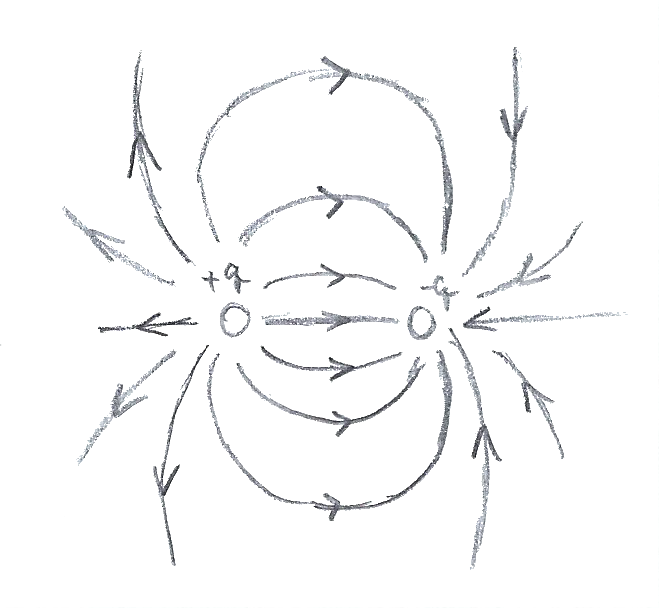
\includegraphics[scale=0.3]{images/em/dipolefield.png}
\end{center}
We will look at the fields of a dipole and its behavior in the problems. 
\subsection{Gauss' Law for Electric Fields}
It turns out that while the principle of superposition is good for finding the electric field, there is an easier way to do so in some symmetric cases. First, we have to talk about the flux of a vector field through a surface. For a flat surface with area $A$, a normal vector to the surface $\hat n$, and a vector field (in this case, the electric field $\vec E$), we have that the flux $\Phi$ through this surface is:
\[
	\Phi = \vec E \cdot \hat n \cdot A
\]
\begin{center}
	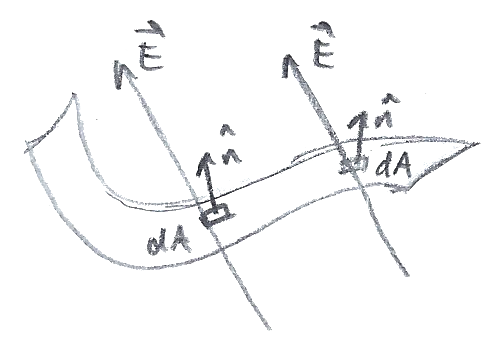
\includegraphics[width=0.3\textwidth]{images/em/electricflux.png}
\end{center}
As you can see from the formula, the flux is a scalar quantity that more or less describes how much a field is flowing through a surface. If the surface in question is not flat, we have to subdivide the surface into many extremely small pieces of area $dA$ that are approximately flat and let the number of pieces go to infinity. We can then calculate the flux $d\Phi$ through each piece:
\[
	d\Phi = \vec E \cdot \hat n \, dA
\]
If we add up all these small amounts of flux, this is what's called a  surface integral, and the flux through some surface $S$ is written as:
\[
	\Phi = \int_S \vec E \cdot \hat n \, dA
\]
If the surface happens to be closed (like a bubble-kind of thing), we draw a circle on the integral sign:
\[
	\Phi = \oint_S \vec E \cdot \hat n\, dA
\]
It's worth mentioning that for closed surfaces (also called Gaussian surfaces) we usually choose the normal vectors to be on the outside or, side of the surface that doesn't have finite volume. (But I'm sure you all know what "outside" means, hopefully, even if you don't go there.)\\
Gauss' Law deals with the electric flux $\Phi_E$ through a closed surface $S$. Specifically, the claim is that the electric flux through a closed surface is proportional to the charge enclosed, written quantitatively as:
\[
	\Phi_E = \oint_S \vec E \cdot \hat n \, dA = \frac{Q_{inside}}{\epsilon_0}
\]
The proportionality constant $\epsilon_0$ is the same one that showed up in Coulomb's constant $k$. \\
Usually, it's impractical to evaluate the surface integral on the left -hand side, so Gauss' Law is usually used to figure out the distributions of charge if the electric field is known. For symmetric cases, however, the flux through some carefully chosen closed surfaces is easy to evaluate, so we can actually derive some electric fields in this manner. Consider first a single charged particle of charge $q$, and say we wish to find the electric field a distance $r$ away from it. We can construct a Gaussian sphere (indicated with the dotted line) with radius $r$ around the particle, and notice that by symmetry, the electric field has to be spherically symmetric and have the same magnitude at the same distances away from the charged particle. \\
\begin{center}
	\begin{asy}
		import graph;
        size(4cm);
        draw(Circle((0, 0), 0.2));
        dot((0,0));
        draw((0,0)--(1.5, 0));
        dot((1.5, 0));
        draw(Circle((0, 0), 1.5), linetype("4 4"));

        label("$q$", dir(60)*0.2, dir(120));
        label("$r$", (0,0)--(1.5,0), dir(90));
	\end{asy}
\end{center}
From this, we can compute the flux as the surface area of the surface times the electric field, or:
\[
	\Phi_E = E \cdot 4 \pi r^2 = \frac{q}{\epsilon_0}
\]
From this we obtain:
\[
	\vec E = \frac{1}{4\pi\epsilon_0} \cdot \frac{q}{r^2} \hat r = \frac{kq}{r^2} \hat r
\]
This is consistent with Coulomb's Law, so Gauss' Law fits in our current framework for electric fields. It turns out that if we run this logic backwards, in a sense, we can also show that Coulomb's Law implies Gauss' Law. \\
In general, though, it still isn't clear that we can apply this to any sort of surface. It turns out that for any convex surface, we can map a sphere to this new convex surface by projecting each patch of area on the sphere to one on the new surface. The flux remains the same through this new patch of area because even though the area of the patch might fluctuate or change based on the square of the distance to the dilation point, the electric field will compensate because it also follows an inverse-square law. Because of this, the size of the convex surface doesn't matter. Furthermore, no charge outside of the surface will contribute anything to the flux, because all the flux of the electric field going into the surface must eventually have the same amount leaving the surface, due to this proportionality. Therefore, it's feasible to have any sort of shape work, even though we won't necessarily be able to use it.\\
There are some special cases that yield easily to Gauss' Law. Let's revisit the infinite line charge with charge density $\lambda$. \\
\begin{center}
    \begin{asy}
        import solids;
        import three;
        size(8cm);
        draw((1, 1, 1)--(0, 1, 1), EndArrow3);
        draw((2, 1, 1)--(3, 1, 1), EndArrow3);
        draw((2, 1, 1)--(1, 1, 1), linetype("2 4"));
        currentprojection=orthographic(0.7, 1, 1);
        currentlight=nolight;
        triple start = (1,1,1);
        real length = 1;
        real radius = 0.5;
        triple ax = (1,0,0);
        revolution r = cylinder(start,radius,length,ax);
        draw(r,black);
        
        draw((2, 1, 1)--(2, 1, 1.5), grey);
        label("$y$", (2, 1, 1.25), dir(180)); 
        draw((2, 2, 1)--(1, 2, 1), linetype("8 8"), EndArrow3);
        draw((1, 2, 1)--(2, 2, 1), linetype("8 8"), EndArrow3);
        label("$L$", (1.5, 2, 1), dir(315)); 
    \end{asy}
\end{center}
Consider a Gaussian cylinder that has its axis of symmetry as the line with length $L$ and radius $y$. The charge enclosed is then $\lambda \cdot L$. Because by symmetry the electric field has to point radially outward, the only flux has to be through the curved side of the cylinder, as no electric field lines pass through the two sides of the cylinder. Furthermore, we know the line of charge should have the same magnitude for the electric field at the same distance from the line charge. With this in mind, we can apply Gauss' Law:
\[
	\oint_S \vec E \cdot \hat n \, dA = E \cdot 2 \pi y L = \frac{\lambda L}{\epsilon_0}
\]
Notice how the $L$ cancels from both sides, leaving us with the electric field:
\[
	E = \frac{\lambda}{2\pi y \epsilon_0} = \frac{2k\lambda}{y}
\]
With Gauss' Law, we can drastically reduce the computation needed for electric fields for symmetric cases, although we do have to be somewhat careful or inventive to deal with these cases. \\ 
\subsection{Electric Potential}
As we discussed when studying mechanics, gravity has a potential energy function and is a conservative force. It turns out that the electromagnetic force is also conservative and has a very similar potential energy function. For a point charge $q$, and assuming the potential energy is zero infinitely far away, we have the potential energy of another charge $q_0$ to be:
\[
	U(r) = -\int_C \vec F \cdot d\vec r = \int_r^{\infty} \frac{kqq_0}{r^2} \, dr = \frac{kqq_0}{r}
\]
Similar to what we did for electric fields, we can define the electric potential $V(r)$ of a charge $q_0$ as the potential energy per unit charge, measured in volts (V):
\[
	V(r) = \frac{U(r)}{q_0} = \frac{kq}{r}
\]
Because of the same division by a charge that we did for electric fields, we can relate the electric field and the electric potential by the following:
\[
	\Delta V = \frac{\Delta U}{q_0} = -\frac{1}{q_0}\int_C \vec F \cdot \, d\vec r = - \int_C \frac{\vec F}{q_0} \cdot d\vec r = -\int_C \vec E \cdot d\vec r
\]
Therefore, we can take the line integral of the electric field to find the potential. Be careful to distinguish between potential energy and potential - potential is energy per unit charge, and is not the same as potential energy, even if their names make it sound like they are the same. \\
Potential follows the principle of superposition as well, but because it is a scalar, there is no need to consider the "direction" of the electric field other than when taking the dot product. For an example, we can revisit the potential of a ring of charge of radius $R$, charge $Q$, and uniform linear charge density $\lambda = \frac{Q}{2\pi R}$. \\
\begin{center}
    \begin{asy}
        import three;
        size(6cm);
        
        triple eye = (7, 8, 5);
        currentprojection = perspective(eye);
        
        triple center = (0, 0, 0);
        real R = 1, y = 2;
        
        draw(circle(center, R, Z));
        dot((0, 0, y));
        
        real dqAngle = -20, dqDelta = 6;
        draw(arc(center, R,
                90, dqAngle - dqDelta,
                90, dqAngle + dqDelta), linewidth(2));
        
        draw(dir(90, dqAngle) -- (0, 0, y), linetype("6 6"));
        
        triple radiusPt = R * dir(90, 170);
        draw((0, 0, 0)--radiusPt, gray(0.2));
        draw((0, 0, 0)--(0, 0, y), gray(0.2));
        
        label("$Q$", (0, R, 0), dir(-90));
        label("$q_0$", (0, 0, y), dir(130));
        label("$dQ$", dir(90, dqAngle), dir(200));
        label("$R$", radiusPt/2, dir(-40));
        label("$y$", (0, 0, y/2), dir(0));
    \end{asy}
\end{center}
For a small arc of the ring, recall that the charge on this portion $dQ = \lambda R \, d\theta$, so the potential $dV$ at a point a distance $y$ above the center of the ring is:
\[
	dV = \frac{k\, dQ}{\sqrt{R^2+y^2}} = \frac{k\lambda R \, d\theta}{\sqrt{R^2+y^2}}
\]
If we integrate with respect to $\theta$ from $0$ to $2\pi$, the integral evaluates to:
\[
	V = \frac{kQ}{\sqrt{R^2+y^2}}
\]
It's important to be able to derive the potentials of the electric fields easily - a table of them for common charge configurations is included at the end. \\
We can also visualize the potential graphically as we did for electric fields. Usually, this is done by drawing a curve connecting all the places where the potential is the same. These lines are called equipotential lines, or if we're in 3-D space, equipotential surfaces. As an example, the blue lines are the equipotentials for the dipole field:
\begin{center}
	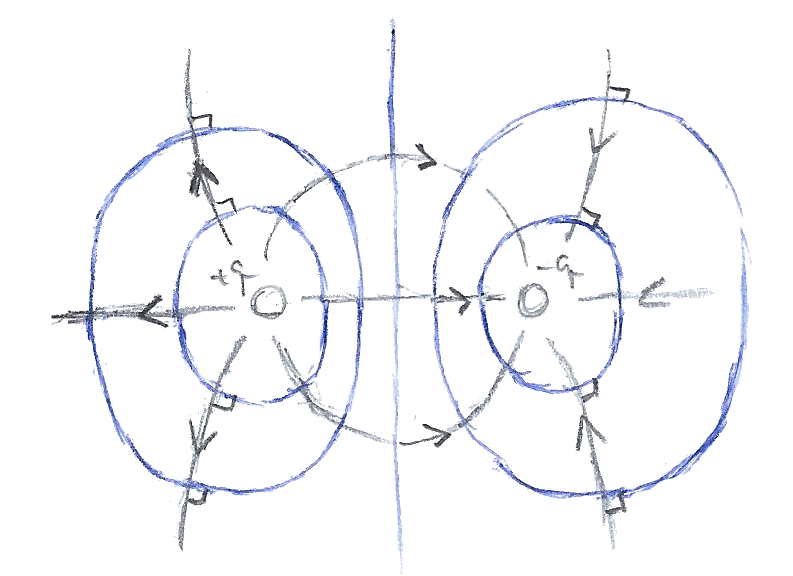
\includegraphics[scale=0.3]{images/em/equipotentials.png}
\end{center}
At equipotentials, the electric force will do no work on the particle as it travels on the surface. Since the electric field points in the direction of the force that does work to push charged particles to lower potentials as well, we can also draw the electric field lines based on equipotential diagrams. 
\subsection{Summary and Problems}
Electrostatics is a huge unit, where we talked about electric charges, fields, potentials, and flux. We first looked at how the electric force between charged objects obeyed an inverse square law, like gravity. We have a lot of tools to look at how stationary electric charges produce electric fields and exert a force on each other - one of our tools is Gauss' Law, a powerful result relating the charge inside a surface to the flux of the field through it. Another powerful tool is the concept of superposition, where we know that electric fields obey vector addition, and we exploited this to find the electric fields of infinitely large/charged objects. We also were able to see that the electric field and force are conservative, and defined potential energy and potential similar to what we did for gravity. The following problems will hopefully try to address all the topics we covered in this unit as well as a little bit of a throwback to mechanics. \\

\noindent \textbf{Problems:}\\
1. (2 $\bigstar$) Two tiny conducting balls of identical mass $m$ and identical charge $q$ hang from nonconducting threads of length $L$, both at an angle $\theta$ to the vertical and from the same point. Assume $\theta$ is so small such that $\tan \theta \approx \sin \theta$. Show that the equilibrium separation of the two balls $x = \left( \frac{q^2L}{2\pi\epsilon_0 mg}\right)^{1/3}$.\\
2. (2 $\bigstar$) A dumbbell consisting of two identical small particles, each of mass $m$, is attached to the ends of a thin (massless) rod of length $a$ that has a pivot at its center. The particles have charges of $+q$ and $-q$, and the dumbbell is located in a uniform horizontal electric field of magnitude $E$, displaced an angle $\theta$ from the horizontal. Show that for small values of the angle $\theta$ between the direction of the dipole and the direction of the electric field, the system displays a rotational form of simple harmonic motion, and show that the period of that motion is $\pi \sqrt{\frac{2ma}{qE}}$. \\
3. (3 $\bigstar$, $\spadesuit$) A thin hemispherical shell of radius $R$ has a uniform surface charge $\sigma$. Show that the magnitude of the electric field at the center of the base of the hemispherical shell is $k\pi\sigma$.\\
4. (4 $\bigstar$) Two positive point charges of charge $+q$ are on the $y$-axis at $y=+a$ and $y=-a$. A bead of mass $m$ and charge $-q$ slides without friction along a taut thread that runs along the $x-$axis. Let $x$ be the position of the bead. a) Show that for $x<<a$, the bead experiences a linear restoring force (a force that is proportional to $x$ and directed toward the equilibrium position at $x=0$) and therefore undergoes simple harmonic motion. b) Show the period of the motion is $2\pi \sqrt{\frac{ma^3}{2kq^2}}$.\\
5. (3 $\bigstar$, $\spadesuit$) A quantum-mechanical treatment of the hydrogen atom shows that the electron in the atom can be treated as a smeared-out distribution of negative charge of the form $\rho(r) = -\rho_0e^{-2r/a}$. Here $r$ represents the distance from the center of the nucleus and $a$ represents the first Bohr radius. Recall that the nucleus of a hydrogen atom consists of just one proton and treat this proton as a positive point charge. Show that $\rho_0 = \frac{e}{\pi a^3}$, where $e$ is the elementary charge, using the fact that the atom is neutral. \\
6. (2 $\bigstar$, $\spadesuit$) All electric dipoles (two charges, one negative and one positive of the same magnitude $q$ a distance $d$ apart) have a dipole moment $\vec p = q \vec d$, where $\vec d$ is the vector pointing from the negative charge to the positive charge. Suppose a dipole is located at a perpendicular distance $R$ from an infinitely long line charge that has a uniform linear charge density $\lambda$. Assume that the dipole moment is in the same direction as the field of the line of charge. Show that the electric force on the dipole is $\frac{2k\lambda p}{R^2}$ if $d << R$.\\
7. (1 $\bigstar$) An infinitely long nonconducting solid cylinder of radius $a$ has a uniform volume charge density of $\rho_0$. Show that the electric field a distance $R$ from the long axis of the cylinder is $E = \frac{\rho_0R}{2\epsilon_0}$ if $0\leq R < a$ and $E = \frac{\rho_0a^2}{2\epsilon_0 R}$ if $R > a$. \\
8. (2 $\bigstar$, $\spadesuit$) A nonconducting solid sphere of radius $R$ has a volume charge density that is proportional to the distance from the center $r$. That is, $\rho = Ar$ for $r < R$, where $A$ is a constant. a) Show the total charge on the sphere is $\pi AR^4$. b) Show that the electric field inside the sphere has magnitude $\frac{Ar^2}{4\epsilon_0}$ and the electric field outside the sphere has magnitude $\frac{AR^4}{4\epsilon_0 r^2}$. \\
9. (3 $\bigstar$) Show that at a point a distance $r$ from the center of a dipole with dipole moment $\vec p$ and charges of magnitude $q$ a distance $L$ apart, we have that the potential $V = \frac{kp\cos \theta}{r^2}$ if $r >> L$ and $\theta$ is the angle between the dipole and the line from the point to the center of the dipole. \\
10. (3 $\bigstar$, $\spadesuit$) Show that the potential inside a uniformly charged solid sphere is given by $V(r) = \frac{kQ}{2R}\left(3 - \frac{r^2}{R^2}\right)$ where $R$ is the radius of the sphere, $Q$ is the charge on the sphere, and $r$ is the distance from the center. (Set $V(\infty) = 0$.)\\
11. (2 $\bigstar$) Four point charges, each with charge $+nq$, are fixed at the corners of a square centered at the origin. The length of each side of the square is $2a$. A fifth particle that has a mass $m$ and a charge $+q$ is placed at the origin and
released from rest. Show that its speed when it is very far from the origin is $v = q\sqrt{\frac{4n\sqrt{2}k}{ma}}$. \\
12. (2 $\bigstar$) A uniformly charged, infinitely long line of negative charge has a linear charge density of $-\lambda$ and is located on the $z$-axis. A small positively charged particle that has a mass $m$ and a charge $q$ is in a circular orbit of radius $R$ in the $xy-$plane centered on the line of charge. Show that the particle is moving at a speed of $v = \sqrt{\frac{2kq\lambda}{m}}$.\\
13. (2 $\bigstar$, $\spadesuit$) Two coaxial conducting cylindrical shells have equal and opposite charges. The inner shell has charge $+q$ and an outer radius $a$, and the outer shell has charge $-q$ and an inner radius $b$. The length of each cylindrical shell is $L$, and $L >> b$. Show the potential difference $\Delta V$ between the two shells is $\Delta V = \frac{2kq}{L}\ln\left(\frac{b}{a}\right)$.\\
14. (3 $\bigstar$) A stationary ring of radius $a$ lies in the $yz$-plane and has a uniform positive charge $Q$. A small particle that has mass $m$ and a negative charge $-q$ is located at the center of the ring. a) Show that if $x$ is the $x$-coordinate of the point and $x<<a$, the electric field at points along the axis of the ring is $-\frac{kQx}{a^3}$. b) Show if the particle is given a small displacement in the $+x$-direction, it will perform simple harmonic motion, and show that the period of the motion is $2\pi \sqrt{\frac{ma^3}{kqQ}}$.
\pagebreak

\section{Conductors and Circuits}
We're going to start talking about things behave when they interact with electric charges, and in general, we classify objects as conductors or insulators based on the ability for charged particles to be transferred across it. For example, insulators like glass and rubber, when charged, don't leak charge to their environment, whereas conductors like metals will, for lack of a better term, conduct charge so that it is spread evenly. When no net charge is flowing from place to place, we say that the conductor has reached electrostatic equilibrium. In this case, the electric field inside the conductor is zero. (This does NOT mean that the potential inside is zero, but rather, is constant - we'll see an example of this). 
\subsection{Ohmic Conductors}
When a potential difference is created across a conductor, electrostatic equilibrium is disrupted and an electric field is created inside the conductor. This causes the flow of charge carriers (electrons) through the conductor, and this flow of charge is called current, usually denoted with an uppercase or lowercase $I$. (I will use the uppercase $I$, because I don't want it to be confused with the imaginary unit.) Current has units of coulombs per second, also called an ampere (A). We also use current density $j$ (a vector quantity), which relates to how the current flows through some cross-sectional area of the solid, and has units of ampere per square meter. The current density vector describes how much current flows through that point inside the solid, and in what direction it flows. The flux of the current density through a surface is the current through that surface - put quantitatively,
\[
	dI = \vec j \cdot \hat n \, dA
\] 
Of course, for non-uniform surfaces, this becomes a surface integral, where you cut up the curved surface into small areas and calculate the current through each area: 
\[
	I = \int_S \vec j \cdot \hat n \, dA
\]
Let's discuss some other properties of the current density. For a conductor of uniform cross section $A$, which has a current flowing through it with uniform current density $j$, we can imagine the current pushing charged particles along at a speed of $v_d$. This is the drift speed of electrons inside the conductor. Notice that we are basically using a fluid to model the flow of charge, like that of water - which is remarkably the truth! Electrons are an incompressible fluid, and don't do weird things like build up in places where they shouldn't - the displacement of one charged particle leads to all of the charge being displaced, which is pretty easy to model.\\
\begin{center}
	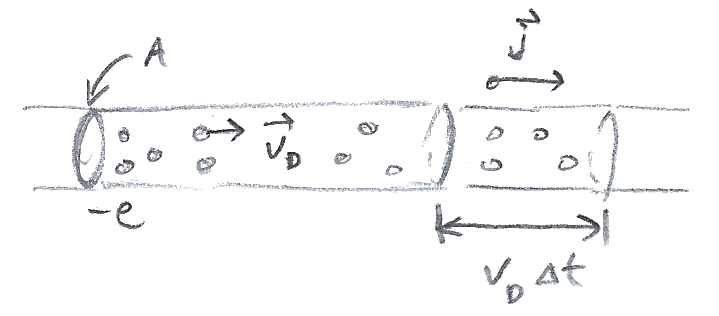
\includegraphics[scale=0.4]{images/em/playdoh.png}\\
\end{center}
In a time $\Delta t$, the volume of the charged particles displaced is $Av_d \Delta t$. The charge pushed through is then the volume times the charge density per unit volume $\rho$. On the other hand, we can express the charge pushed through directly in terms of the current $I = jA$. The charge moved in a time $\Delta t$ is just $I\Delta t = jA \Delta t$. We can equate this and get:
\[
	Av_d\Delta t \rho = jA\Delta t \rightarrow 	v_d \rho = j 
\]
Sometimes we will also see $n$, the number density of charged particles per cubic meter, and usually, we'll see electrons flowing, so we'll see the charge $e$ as well in this equation. Notice that in terms of magnitude, we have $\rho = en$, so 
\[
	j = v_d en
\]
We can also express this in vector form: it is also true that 
\[
	\vec j = -en \vec v_d
\]
We have to be careful, however - if the charges of the particles are negative, as is the case for electrons, then the drift velocity of the electrons are in the opposite direction as the current. Therefore, it's from this that I have to warn you - even though we may know the direction of the current in a wire, without other information we can't tell whether or not the current consists of positively-charged particles moving in the direction of the current or negatively-charged particles moving opposite to it. \\
It turns out that the current density is also directly related to the electric field for some conductors, through a relation called Ohm's Law. This isn't the regular form of Ohm's Law that you're used to, it's the differential form - but we'll see how to get there from the differential form. \\
Ohm's Law (differential form) states that 
\[
	\vec j = \sigma \vec E
\]
In this case, $\sigma$ is not the charge density, it's the proportionality constant called the conductivity of the material. Conductors that follow this rule are called ohmic conductors, and a large number of conductors follow this rule (not in extreme cases). \\
\begin{center}
	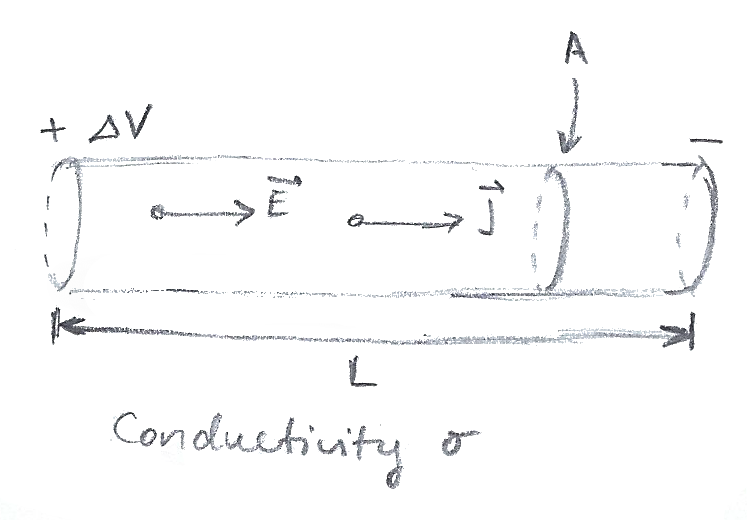
\includegraphics[width=0.4\textwidth]{images/em/ohmic-conductor.png}\\
\end{center}
For simplicity, let's assume we have a conductor with length $L$ and uniform cross section $A$, and that this electric field $E$ is created from exerting a constant potential difference $\Delta V$ across the ends of the conductor. Let's also just consider the magnitudes of the current density and electric field and multiply through on both sides by the volume of the conductor, $LA$:
\[
	L A j = \sigma E L A
\]
We can group the terms in certain ways to get the potential difference $\Delta V$ and the current $I$. Namely, the potential difference $\Delta V = EL$, and the current $I = jA$, so substituting we have:
\[
	LI = \sigma A \Delta V
\]
We can now isolate $\Delta V$:
\[
	\Delta V = I \frac{L}{A\sigma} = IR
\]
This fractional term that appears is defined as the resistance $R$ of the object. Resistance, as you may know, is measured in ohms ($\Omega$).  For the cases we will consider on a regular basis, this is sufficient. Sometimes it's written like this:
\[
	R = \frac{L}{A}\rho
\]
where $\rho = \frac{1}{\sigma}$ is the resistivity of the object. This, along with the above, gives us enough relations to be able to calculate most properties of a conductor given some information. 
\subsection{Capacitance}
Capacitance is a property of conductors that indicates the ability to store charge due to a potential difference. If two separated conductors are charged to $+Q$ and $-Q$, respectively, by a potential difference of $V$, then the capacitance $C$ of this system is given by 
\[
	C = \frac{Q}{V}
\]
This system of two conductors is called a capacitor, and the capacitance of a capacitor is measured in farads (F), named after Michael Faraday. It turns out the capacitance of a capacitor is dependent only upon the geometry of the system and the permittivity of free space $\epsilon_0$ (unless there's a material that's not air between the two conductors, which we will discuss later). This seems unlikely - but we can show that this is true intuitively. \\
Consider that on the surface of these two conductors the magnitude of the charge of each of them is doubled. Therefore, since the electric field generated by the conductors is proportional to the charge of the source of the field, therefore the electric field must be doubled. Because of this, the potential difference between the two capacitors also doubles, and since the potential difference and charge scale up by the same amount when the charge changes, the ratio between them remains constant. So, the capacitance remains constant independent of the charge of the conductors, so it must be dependent on the configuration of the system (geometrically) and the permittivity $\epsilon_0$. One can see that the unit for a farad and the units of $\epsilon_0$ differ by a factor of a meter, and one can often write $\epsilon_0$ as 8.854 $\cdot$ 10$^{-12}$ F/m, as it's the cleanest way to write the units. \\
In order to charge the capacitor, energy clearly needs to be input in order to move charge from one conductor to the other in order to create this imbalance. We can calculate the total energy required to move a total charge $Q$ from one conductor to the other. For a small charge $dq$, the amount of work needed to move against the potential difference $V(q) = \frac{q}{C}$ is 
\[
	dW = V(q) \, dq = \frac{q}{C} \, dq
\]
We can integrate from $0$ to $Q$: 
\begin{align*}
	W &= \int_0^Q \frac{q}{C} \, dq \\
	&= \frac{1}{2} \frac{q^2}{C} \Big|_0^Q\\
	&= \frac{1}{2} \frac{Q^2}{C} = \frac{1}{2}QV = \frac{1}{2}CV^2
\end{align*}
This energy is stored in the capacitor as potential energy, and in fact, it's stored in the electric field generated by this imbalance of charge. The electric field has an energy density per unit volume within it - it turns out that this energy density $u = \frac{1}{2}E^2 \epsilon_0$, but knowing how this formula is derived is beyond the scope of this course.\\
The most common capacitor we will encounter is the parallel-plate capacitor. It's two squares of charge with area $A$ and surface charge density $\sigma$, and whose plates are separated by a distance $d$.
\begin{center}
	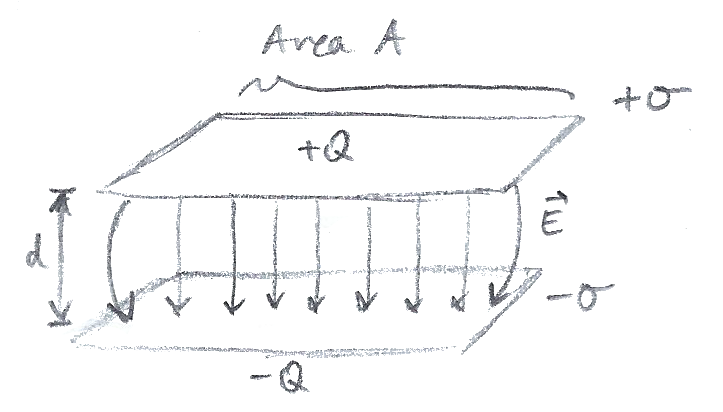
\includegraphics[width=0.4\textwidth]{images/em/capacitor.png}
\end{center}
From electrostatics, since each plane contributes a field of $\frac{\sigma}{2\epsilon_0}$ to the electric field, the total electric field is $\frac{\sigma}{\epsilon_0}$. (These fields don't cancel each other out as the field lines point the same direction). We can effectively consider the plates as planes of charge, even though they are finite. Only at the edges of the capacitor does the electric field become non-uniform, so approximately speaking, far from the edges of the planes, this is true. Even with this in mind, we can derive the potential difference as $V = \frac{\sigma d}{\epsilon_0}$. The charge on each capacitor plate is $Q = \sigma A$, so then the capacitance $C$ is:
\[
	C = \frac{Q}{V} = \frac{\sigma A}{\frac{\sigma d}{\epsilon_0}} = \frac{A \epsilon_0}{d}
\]
The energy stored in the field of the capacitor can then be found to be:
\[
	U = \frac{1}{2}QV = \frac{1}{2} \sigma A \frac{\sigma d}{\epsilon_0} = \frac{\sigma^2 Ad}{2\epsilon_0}
\]
The density of this field, according to our formula, is:
\[
	u = \frac{1}{2} \epsilon_0 \left(\frac{\sigma}{\epsilon_0}\right)^2 = \frac{\sigma^2}{2\epsilon_0}
\]
And observe that if we multiply through by the volume, $Ad$, the correct expression for the energy stored appears, confirming the consistency of the energy density formula for this particular case (which is still true in general). \\
We can now discuss the more complicated case if something is inserted between the two conductors. In this case, the insertion of some solid increases the permittivity in the object by a scalar $\kappa$, called the dielectric constant. The new object's permittivity $\epsilon = \kappa \epsilon_0$. This, in turn, increases the capacitance of the capacitor by the same constant $\kappa$, so the new capacitance $C_f$ as compared to the original, $C_i$, is:
\[
	C_f = \kappa C_i
\]
Simple enough. Usually this constant is obtained by measurement, so the dielectric constant will be given most of the time. Since a dielectric changes the permittivity of the space between the plates from $\epsilon_0$ to $\epsilon = \kappa \epsilon_0$, this means that the electric field weakens by a factor of $\kappa$ inside the dielectric material. Charges are induced on the surface of the dielectric of the opposite sign as the charge on the closer plate, because the charges on the capacitor plates polarize the material. Note that the combined charges on the capacitor plate and on the surface of the dielectric should produce the total electric field in the material. Since the electric field strength decreases by a factor of $\frac{1}{\kappa}$, the total charge of the plate and the dielectric is $\frac{1}{\kappa}$ times the original and therefore the charges induced on the surface of the dielectric must have magnitude  $1 - \frac{1}{\kappa}$ and of the opposite sign in order to align with this. \\
As far as capacitors go, they store energy in an electric field. We'll soon see their behavior in circuits, where they will be a complication to the resistor-only circuits seen in Design and Tech. 
\subsection{Circuits and Kirchhoff's Laws}
The culmination of talking about conductors and their properties is their application in building and analyzing circuits. In a closed circuit, there is always some way where a potential difference $V$ is exerted on the wire that allows electrons to travel through it, creating a current. The most common way this is done is by a constant source of electrical energy, like a battery, that produces an electromotive force (emf) $\mathscr{E}$. In a circuit, the main circuit component that provides resistance are resistors, and the main component that provides capacitance to the circuit is the capacitor, as discussed earlier. We will later discuss a quantity called inductance and another circuit element, inductors, but not until we talk about magnetism. \\
A short digression on batteries - as you might remember from chemistry, batteries are powered by a redox reaction that creates a potential difference between the two electrodes of the battery. As electrons pass from the negatively charged electrode to the positively charged electrode, the anode (-) becomes more and more negatively charged, and the cathode (+) becomes more and more positively charged. Eventually, the negative ions will be depleted and therefore the battery will decrease in its potential until it reaches 0. Ideally, however, we will deviate from reality and assume our batteries will maintain a constant emf $\mathscr{E}$. Furthermore, since everything has some internal resistance, we sometimes might add a small resistor $r$ to a circuit to model this internal resistance. \\
Another assumption that we make regarding a circuit is that the conductor through which electrons flow, the wire, has negligible internal resistance. Of course, this is not true because we can calculate it using ideas from our analysis of conductors and their properties, but we will omit it when discussing circuits. \\
The most important rules that we can use to analyze circuits is Kirchhoff's Loop Rules. There are only two:\\
Kirchhoff's Voltage Law (KVL):  Around a closed loop, the sum of the potential differences is zero. \\
Kirchhoff's Current Law (KCL): At a junction in a circuit, the total current going in is equal to the total current going out. \\
These can be derived from principles we already know. For KVL, recall that because the electric force is conservative, we have that the line integral of the force on a charged particle around a closed loop is zero. Considering this expression per unit charge, we have:
\[
	\oint_C \vec F \cdot \, d\vec s = 0 \rightarrow \oint_C \vec E \cdot \, d\vec s = 0
\]
However, this is the same as looking at the potential around a closed loop, so this too is zero. For KCL, we can notice that because charge is conserved, all of the charge that flows into a junction must flow out. \\
We can use these rules to look at capacitors and resistors in series and parallel before moving to analyze our first (time-dependent!) circuit. As a reminder, "series" refers to on the same branch, while "parallel" refers to on different branches. \\
First, we can take a look at these circuit components in parallel. (Our derivations here can be extended to more than two capacitors/resistors.)\\
For two capacitors in parallel with capacitances $C_1$ and $C_2$, and a voltage $V$ across the system, we can try to calculate the total capacitance of the system. Assume that the charge on each of these capacitors, when fully charged, are $Q_1$ and $Q_2$, respectively. The capacitance of a capacitor $C$ that would have the same capacitance as these two capacitors in parallel would be:
\[
	C = \frac {Q^{tot}}{V}
\]
Notice that $Q^{tot} = Q_1 + Q_2$ by conservation of charge. We can then split this:
\[
	C = \frac{Q_1}{V} + \frac{Q_2}{V}
\]
As the voltage across each branch is the same as the voltage across the system, we have that:
\[
	C = \frac{Q_1}{V_1} + \frac{Q_2}{V_2} = C_1 + C_2
\]
We can do a similar analysis for resistors. For two resistors in parallel with resistances $R_1$ and $R_2$, and currents $I_1$ and $I_2$ across each resistor, we can look at the total resistance $R$ in terms of Ohm's Law:
\[
	R = \frac{V}{I}
\]
where $I$ is the total current going into/out of the branches. By Kirchhoff's Current Law, $I = I_1 + I_2$, and so we can make this substitution:
\[
	R = \frac{V}{I_1 + I_2} = \frac{1}{\frac{I_1+I_2}{V}}
\]
We can re-apply Ohm's Law on the denominator:
\[
	R = \frac{1}{\frac{I_1}{V} + \frac{I_2}{V}} = \frac{1}{\frac{I_1}{V_1} + \frac{I_2}{V_2}} = \frac{1}{\frac{1}{R_1} + \frac{1}{R_2}}
\]
Rearranging, we have:
\[
	\frac{1}{R} = \frac{1}{R_1} + \frac{1}{R_2}
\]
We can repeat this for capacitors and resistors in series. For a system of two capacitors with capacitances $C_1$ and $C_2$, and a voltage $V$, we can imagine a capacitor with capacitance $C$ equal to the total capacitance of both capacitors. The voltage drop for each capacitor $V_1$ and $V_2$ sum to the total voltage $V$, so $V_1 + V_2 = V$. The charge on each capacitor $Q_1$ and $Q_2$ are both equal to the total charge through the system $Q$ since the current is the same going through both capacitors. We can calculate the capacitance now:
\[
	C = \frac{Q}{V} = \frac{Q}{V_1+V_2} = \frac{1}{\frac{V_1+V_2}{Q}} = \frac{1}{\frac{V_1}{Q} + \frac{V_2}{Q}} = \frac{1}{\frac{V_1}{Q_1} + \frac{V_2}{Q_2}} = \frac{1}{\frac{1}{C_1} + \frac{1}{C_2}}  
\]
The most compact way to write this is:
\[
	\frac{1}{C} = \frac{1}{C_1} + \frac{1}{C_2}
\]
For two resistors $R_1$ and $R_2$ with current $I_1$ and $I_2$ across them, we can find the total resistance $R$ using Ohm's Law, noting that the total current $I = I_1 = I_2$:
\[
	R = \frac{V}{I} = \frac{V_1 + V_2}{I} = \frac{V_1}{I} + \frac{V_2}{I} = \frac{V_1}{I_1} +  \frac{V_2}{I_2} = R_1 + R_2
\]
With these relations to condense resistors/capacitors in series and in parallel, we can now always effectively condense circuits to one resistor and one capacitor. Let's analyze the simplest 1-loop circuit with a resistor and a capacitor - the simplest RC circuit.
\begin{center}
	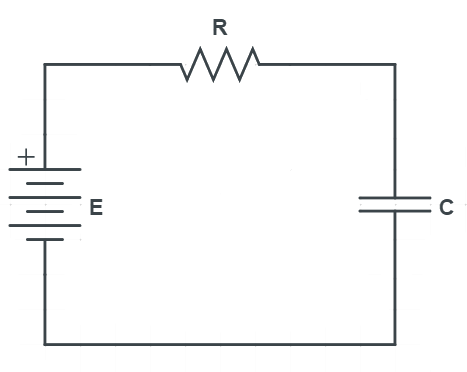
\includegraphics[scale=0.25]{images/em/RC-circuit.png}
\end{center}
Consider a battery with emf $\mathscr{E}$, a resistor with resistance $R$, and a capacitor with capacitance $C$. Let $Q$ denote the charge on the capacitor as a function of time and $I$ the current. When the switch is initially flipped to complete the circuit, assume no charge lies on the plates of the capacitor. From KVL, we have, at any given moment:
\[
    \mathscr{E} - IR - \frac{Q}{C} = 0
\]
Noting that $I = \frac{dQ}{dt}$, we can rewrite this as our first first-order differential equation:
\[
    \mathscr{E} - R\dv{Q}{t} - \frac{Q}{C} = 0 
\]
\[
    R\dv{Q}{t} =  \frac{\mathscr{E}C - Q}{C}  
\]
\[
    \frac{RC}{\mathscr{E}C-Q}\dv{Q}{t} = 1
\]
Integrating from time $t=0$ to arbitrary time $t$, we have:
\[
    \int_0^t\frac{RC}{\mathscr{E}C-Q}\dv{Q}{t}\, dt = \int_0^t 1 \, dt
\]
\[
    -RC \ln\left(\frac{\mathscr{E}C-Q(t)}{\mathscr{E}C}\right) = t
\]
\[
    \mathscr{E}C-Q(t) = \mathscr{E}Ce^{-\frac{t}{RC}}
\]
\[
    Q(t) = \mathscr{E}C\left(1-e^{-\frac{t}{RC}}\right)
\]
We can take the derivative to find the current $I$:
\[
	I = \dv{Q}{t} = \dv{}{t} \mathscr{E}C\left(1-e^{-\frac{t}{RC}}\right) = \frac{\mathscr{E}}{R}e^{-\frac{t}{RC}}
\]
When the circuit is closed at time $t=0$, the current $I = \frac{\mathscr{E}}{R}$, which is basically the same as if there was no capacitor and instead just a wire. In general, at the beginning of the charging of a capacitor, the capacitor acts like a wire. As $t \to \infty$ and approaches the steady state, the charge on the capacitor approaches $\mathscr{E} C$, and the current approaches zero. This is because the energy from the voltage that the capacitor extracts from the circuit is stored into the electric field of the capacitor, and eventually this will force the current to decrease as to satisfy KVL. The resistor, on the other hand, extracts energy from the circuit and converts it into vibrations and heat energy that is released and not stored.\\
The time it takes for this process of charging the capacitor to occur is influenced by the magnitudes of $R$ and $C$.  In fact, RC circuits have a time constant $\tau = RC$ that serves as a measure of how fast/slow the circuit is charged. (Note: the time constant has units of seconds - in fact, an ohm-farad is a second. You can verify this by dimensional analysis.)\\
Sometimes we will be asked what the power through a component in a circuit is at a given moment. The power is simply the voltage difference across the component times the current flowing through it. If we are able to express the power as a function of time, we will be able to integrate it (hopefully) to find the energy dissipated/stored/released over a time interval, which is useful for keeping track where the energy goes in a circuit. 
\subsection{Summary and Problems}
This chapter covered a wide variety of topics, starting with the ability of conductors to conduct current, and identifying properties of conductors such as their conductivity, resistance, and capacitance. We also looked at our first circuits and looked at how to model the behavior of a circuit over time. Most of these problems will be either circuit problems (harder) or calculating a property of a conductor (easier).\\

\noindent\textbf{Problems:}\\
1. (1 $\bigstar$) Show the resistivity of a long straight wire of radius $r$ and length $L$ is $\frac{\Delta V\pi r^2}{IL}$, if $I$ is the current through the wire when a potential difference of $\Delta V$ is exerted across the ends of the wire.\\
2. (2 $\bigstar$) The electric field at point $P$ just outside the outer surface of a hollow spherical conductor of inner radius 10 cm and outer radius 20 cm has magnitude 455 N/C and is directed outward. When an unknown point charge Q is introduced into the center of the sphere, the electric field at P is still directed outward but is now 185 N/C. Show that the total charge on the inside surface of the shell is 1.20$\cdot$10$^{-9}$ C.\\
3. (1 $\bigstar$) The magnitude $J$ of the current density in a certain wire with a circular cross section of radius $R$ = 2.10 mm is given by $J$ = (4.00$\cdot$10$^8$)$r^2$, with $J$ in amperes per square meter and radial distance $r$ in meters. Show that the current through the outer section bounded by $r = 0.690R$ and $r = R$ is 9.45 mA.\\
4. (3 $\bigstar$) A metal ball with radius $R$ carries a total charge $Q$. The ball is surrounded by a thick conducting shell of inner radius $2R$ and outer radius $3R$. The total charge on the shell is zero and the conductors are in electrostatic equilibrium. Show that the electric potential of the metal ball relative to zero potential at infinity is $\frac{5kQ}{6R}$.\\
5. (4 $\bigstar$) A parallel plate capacitor of plate area $A$ and plate separation $d$ has a potential difference of $V_0$ is applied between the plates. Suppose that the battery remains connected while a dielectric slab of thickness $b$ and dielectric constant $\kappa$ is being introduced exactly between the two plates of the capacitor. Show that the electric field in the slab is $E = \frac{V_0}{\kappa d - (\kappa -1) b}$.\\
6. (3 $\bigstar$) The space between two concentric conducting spherical shells of radii $b$ and $a$ ($b>a$) is filled with a substance of dielectric constant $\kappa$. A potential difference $\Delta V$ is applied across the inner and outer shells. Show that the magnitude of the induced charge along the surface of the inner shell is $\frac{\Delta V 4\pi \epsilon_0 ab (\kappa -1)}{\kappa(b-a)}$.\\
7. (2 $\bigstar$) A charged isolated metal sphere of diameter $d$ has a potential $V$ relative to $V=0$ at infinity. Show that the energy density in the electric field near the surface of the sphere is $\frac{2V^2\epsilon_0}{d^2}$.\\
8. (2 $\bigstar$) A parallel-plate capacitor has plates of area $A$ and separation $d$ and is charged to a potential difference $V$. The charging battery is then disconnected, and the plates are pulled apart until their separation is $2d$. Show that the work required to pull these plates apart to this separation is $\frac{\epsilon_0AV^2}{2d}$.\\
9. (3 $\bigstar$, $\spadesuit$) A switch in an RC circuit is closed at time $t=0$, to begin charging an initially uncharged capacitor of capacitance $C$ through a resistor of resistance $R$. Show that in $RC \ln 2$ seconds, the voltage across the resistor will be the same as the voltage across the capacitor.\\
\begin{center}
	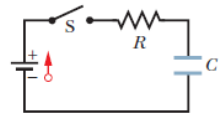
\includegraphics[scale=0.7]{images/em/RC-problem1.png}
\end{center}
10. (3 $\bigstar$) In the figure below, $R_s$ is to be adjusted in value by moving the sliding contact across it until points $a$ and $b$ are brought to the same potential. (One tests for this condition by momentarily connecting a sensitive ammeter between $a$ and $b$; if these points are at the same potential, the ammeter will not deflect.) Show that when this adjustment is made, we have that $R_x = \frac{R_sR_2}{R_1}$. \\
\begin{center}
	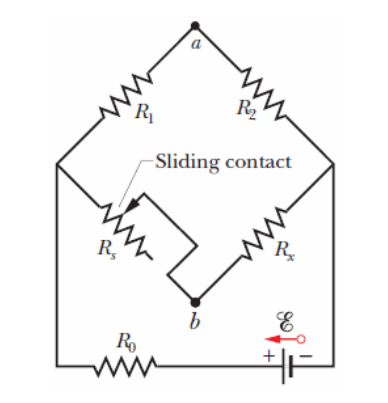
\includegraphics[scale=0.7]{images/em/circuit-problem1.png}
\end{center}
11. (2 $\bigstar$, $\spadesuit$) For the RC circuit shown in the figure below, the switch is initially closed to contact $a$. After having been at contact $a$ for a long time, the switch
throw is rotated to contact $b$. Once this happens, show that the charge on the capacitor can be modeled as a function of time as $Q(t) = \mathscr{E}Ce^{-t/RC}$.
\begin{center}
	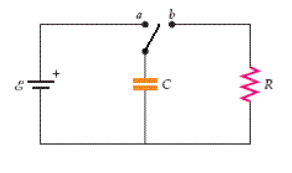
\includegraphics[scale=0.7]{images/em/RC-problem2.png}
\end{center}
12. (2 $\bigstar$) Using the same diagram at problem 11, show that the energy stored in the capacitor $U$ can be modeled as a function of time as $U(t) = \frac{1}{2}\mathscr{E}^2Ce^{-2t/RC}$.\\
13. (3 $\bigstar$) A cylindrical capacitor with an air gap has an inner radius of $r$, a thin outer shell with radius $R$, and length $L$. The capacitor is charged to a voltage difference of $\Delta V$. Show that the minimum energy density stored in the gap when the capacitor is fully charged is $\frac{1}{2} \epsilon_0 \left(\frac{\Delta V}{R\ln(r/R)} \right)^2$. \\
14. (3 $\bigstar$) Switch $S$, shown in the figure below, is closed after having been open for a long time. Show that the charges on the capacitors are 130 $\mu$C and 260 $\mu$C a long time after the switch has been closed. 
\begin{center}
	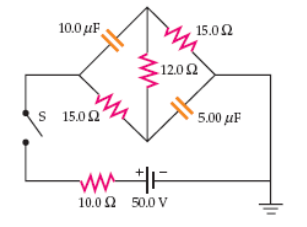
\includegraphics[scale=0.7]{images/em/RC-problem4.png}
\end{center}
\pagebreak

\section{Magnetism}
Up until this point we haven't taken much of a  look at the behavior of charges in motion, or the magnetic field and how it is related to the electric field. The symbol we will use for the magnetic field is $\vec B$ (because apparently, the letter M is just too common), and the magnetic field is measured in units of teslas (T). However, a 1 T magnetic field is really strong (for context, the Earth's magnetic field has a strength of 0.25-0.65 microteslas). We also define the gauss, which is $10^{-4}$ teslas, which we will also use to measure the strength of magnetic fields. We will look at how we can calculate this field, how it arises and interacts with charges, and how a changing magnetic field can actually induce, or create an electric field. 
\subsection{Lorentz Force}
Up until this point, we've only talked about the electric force on a charged particle, where $\vec E = \frac{\vec F}{q}$ or $\vec F = q\vec E$. This is not the full picture - the magnetic field also exerts a force on charged particles, and the full expression for the electromagnetic force on a charged particle (the Lorentz force) is the following:
\[
	\vec F = q\vec E + q\vec v \times \vec B
\]
This second term is the magnetic force on a charged particle, which is dependent on the velocity of the particle. This dependency means that the magnetic force is non-conservative - it cannot have a potential energy function because it is dependent on factors other than the position of the particle. However, the magnetic force also does no work on a charged particle - to see this, notice that the magnetic force always acts perpendicular to the direction that the force is moving, so the dot product, when evaluated, will be zero. This is strange - the magnetic force does not do work on a charged particle but is non-conservative, but that's just how it works. There is such a thing as magnetic (vector and scalar) potential - but there's no need to worry about that.\\
When we deal with magnetic forces, we usually deal with relatively simple cases. The first is the case of a "velocity selector" - the setup is a region where the electric field $\vec E$ and magnetic field $\vec B$ are perpendicular to each other and let's say that a beam launches (positively) charged particles at various velocities through this region. What velocity-particles will not be deflected by the electromagnetic field? \\
\begin{center}
	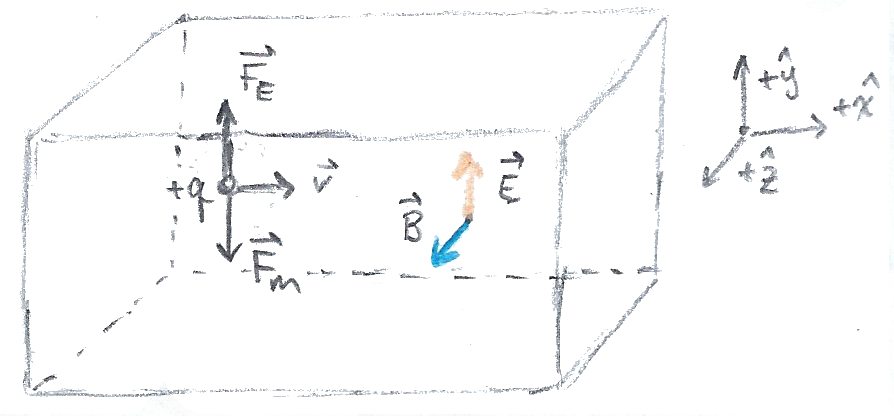
\includegraphics[width=0.5\textwidth]{images/em/velocity-selector.png}
\end{center}
To find this out, we can assume that the velocity is in the $+x$-direction, the electric field is in the $+y$-direction, and the magnetic field is in the $+z$-direction. In order for the motion of the particle to remain unchanged, the force must be zero. \\
Before we do any calculations, let's figure out if this is possible by checking the directions of the two forces. The electric force must be in the $+y$-direction, as the electric field and the electric force are proportional, and the magnetic force must be in the direction that $\hat x \times \hat z$ points in. Using the right-hand rule, this points in the $-y$-direction, so we're sure that this is possible. (If they didn't point in opposite directions, we'd be screwed.)\\
At this point, we can just compare the magnitudes of the electric and magnetic forces. The magnitude of the electric force is $qE$, while the magnitude of the magnetic force is $qvB$. If we set these equal, we find the desired velocity to be $v = \frac{E}{B}$. \\
Another common scenario is circular motion due to a magnetic field. Suppose a particle is launched with velocity $\vec v$ up the page in a uniform magnetic field $\vec B$ into the page, and the particle has mass $m$ and charge $q$. The motion of the particle will be circular - and it'll be uniform as well. 
\begin{center}
	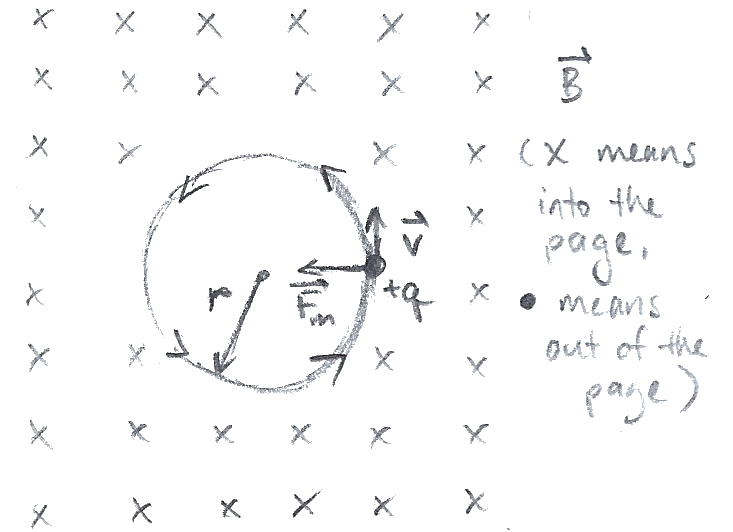
\includegraphics[scale=0.25]{images/em/magnetic-circles.png}
\end{center}
We can find the radius of the motion based on our givens. Using Newton's Second Law (and that the acceleration of a particle in UCM is $\frac{v^2}{r}$, if $r$ is the radius, then we have that:
\[
	m\frac{v^2}{r} = qvB
\]
This rearranges to 
\[
	r = \frac{mv}{qB}
\]
It turns out that the period of this motion is independent of the velocity or radius of the motion. To show this, we can use Newton's Second law to find $\omega = \frac{v}{r}$, which is the angular velocity of the motion:
\[
	\omega = \frac{v}{r} = \frac{q}{m}B
\]
From here, since $T = \frac{2\pi}{\omega}$, we have that 
\[
	T = \frac{2\pi m}{qB}
\]
We can use this to calculate the charge-to-mass ratio of the particle being launched easily since we can control the magnitude of the magnetic field being applied. \\
One last application: what about the magnetic force on a wire due to a current flowing through it? After all, electrons are moving in the wire and can't be dislodged from it, so there is definitely a magnetic force on it. For simplicity, consider a uniform magnetic field $\vec B$, a current $I$ in the wire, and let the wire be straight and have length $L$, have cross-sectional area $A$, and let the number density of electrons per cubic meter be $n$. \\
\begin{center}
	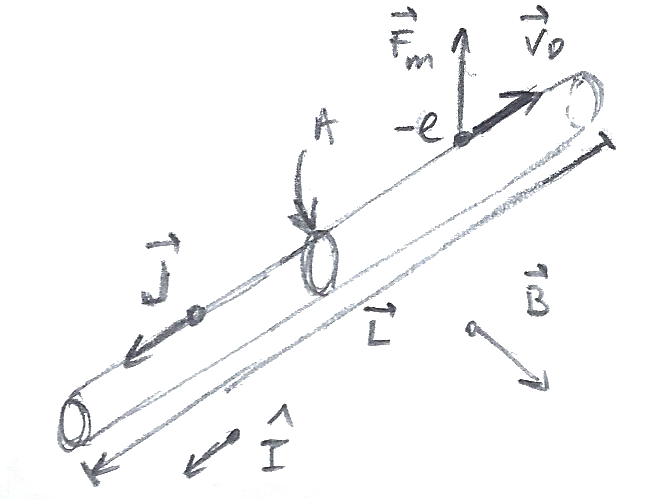
\includegraphics[scale=0.2]{images/em/magnetic-force-wire.png}
\end{center}
On a single charge in the wire drifting along with drift velocity $\vec v_D$, and we can find the magnetic force on each electron (with charge $-e$!):
\[
	\vec F_m = -e\vec v_D \times \vec B
\]
How many electrons are there? It's the volume of the wire times the number density per cubic meter $n$, which is $LAn$. This means the total force $\vec F$ is:
\[
	\vec F = -LAne\vec v_D \times \vec B
\]
We can relate this to the current $I$ - remember that in a conductor we know the current density $\vec j$ is:
\[
	\vec j = -en \vec v_D
\]
Because the charges are negative, they flow OPPOSITE to the current, so $\vec j$ is going in the same direction as the current. We can substitute this in:
\[
	\vec F = AL \vec j \times \vec B
\]
The current and the current density are in the same direction in this straight wire, so let's define a unit vector in that direction $\hat I$. Let's just rewrite this as:
\[
	\vec F = ALj \hat I \times \vec B
\]
Recall that the current $I = jA$ for these uniform wires. Let's have $\vec L = L \hat I$ be the displacement vector along the wire. 
\[
	\vec F = I\vec L \times \vec B
\]
We did this instead of the vector representing the current in the wire because we can actually integrate on the length vectors. For an arbitrary uniform wire, we can look at the differential force $d\vec F$ on the wire by the magnetic field:
\[
	d\vec F = Id\vec l \times \vec B
\]
When we sum up all of these forces:
\[
	\vec F = \sum d\vec F = \sum I d\vec l \times \vec B = I \sum d\vec l \times \vec B
\]
For a current loop, this vector sum becomes zero, because the net displacement around the loop is zero, so the entire product becomes zero. However, there is a torque on this loop. For a small loop of area $A$ and current $I$, define the magnetic moment of the loop to be $\vec \mu = IA\hat n$, where $\hat n$ is the normal unit vector to the plane of the loop. In a uniform magnetic field $\vec B$, it can be shown that the torque on this loop is $\tau = \vec \mu \times \vec B$. This torque tends to line up the magnetic moment with the magnetic field. This motion actually has a potential energy associated with it where $U = -\vec \mu \cdot \vec B$. These are all things that are useful but are just too complicated to prove. \\
There are many other applications for magnetic fields that haven't been discussed, and we'll explore some of them in the problems. 
\subsection{Biot-Savart and Ampere's Laws}
Magnetic fields are induced as a result of the motion of charges - macroscopically, this means currents and its distribution. When we look at magnetic field lines, qualitatively, they form closed loops, unlike that of electric fields due to charges - this can be easily seen by sprinkling a magnetizable material, such as iron shavings, near a magnet. Because the magnetic field lines are closed, it's hard to indicate a direction in which the field lines are going (ie. clockwise or counterclockwise) but we use the right-hand-rule as the arbitrary guideline in this case. For dipoles like magnets, the rule is that the field lines come out from the north pole, loop around the magnet, pass through the south pole and through the body of the magnet to close the loop.\\
\begin{center}
	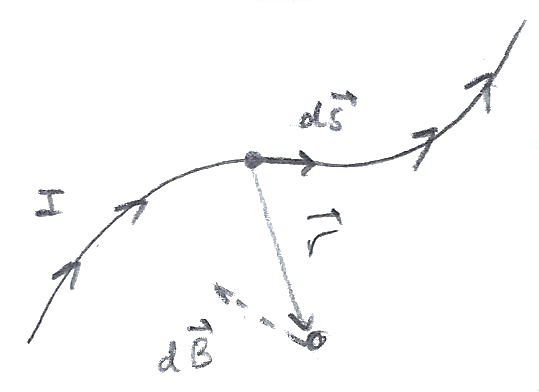
\includegraphics[width=0.4\textwidth]{images/em/biot-savart.png}
\end{center}
Biot and Savart quantitatively derived the magnetic field vector at a point due to a current, and the law used to describe the magnetic field is called (surprise) the Biot-Savart Law. For a uniform length of stationary current that moves $d\vec s$ and $\vec r$ is the displacement vector from the current to the point at which the magnetic field is being calculated, we have that the magnetic field due to this small current is:
\[
	d\vec B = \frac{\mu_0}{4\pi} \frac{I \, d\vec s \times \hat r}{r^2}
\]
where $I$ is the current at that point. The proportionality involves a constant $\mu_0$ that we haven't yet seen - it's called the permeability of free space and has a value of exactly $4 \pi \cdot 10^{-7}$ T$\cdot$m/A. (Alternatively, 1.26 $\cdot$ 10$^{-6}$ T$\cdot$m/A will do just fine.) Similar to Coulomb's Law, Biot-Savart can be used to superpose magnetic fields to calculate the overall magnetic field, and it also follows an inverse-square law similar to that of Coulomb's Law. Therefore, Biot-Savart is useful for calculating the magnetic field due to a complicated configuration of currents, but we can apply it to basically anything - and I'll present the calculations for the field due to an infinite line of current.\\
\begin{center}
    \begin{asy}
        import geometry;
        size(9cm);
        
        real y = 5;
        dot((0, y));

        draw((0,0)--(-10,0), linetype("4 4"), Arrow);
        draw((5.5,0)--(10,0), linetype("4 4"), Arrow);
        draw((-4.25,0)--(0,y), linetype("6 6"));
        draw((0, y)--(0,0));
        draw((-4,0)--(-4.5,0), linewidth(2));
        draw((0,0)--(5.5,0), linetype("4 4"), Arrow);

        label("$y$", (0, y/2), dir(0));
        label("$x$", (-2, -0.5), dir(270));
        label("$dx$", (-4.25, -0.5), dir(270)*0.2);
        label("$I$", (5.5, 0), dir(50));
        label("$P$", (y,0), dir(130));
    \end{asy}
\end{center}
Consider a point $P$ that is a distance $y$ from a uniform line of current carrying a current $I$. Like with the infinite line charge, we can superimpose the real number line on the charge, having the foot of the perpendicular from the point to the line be $x=0$ and extending out to infinity in both directions. Let's arbitrarily have the current running in the $+x$-direction (it won't change the magnitude of the final answer). \\
We know that the magnetic field lines circulate around the current, and the magnitude of the magnetic field due to a small piece of current at a position $x$ going through a displacement $d\vec x$ is:
\[
	d\vec B = \frac{\mu_0}{4\pi} \frac{I \, d\vec x \times \hat r}{x^2+y^2}
\]
Note that all of these small contributions to the field are going to be in the same direction - after all, all of these vectors will be perpendicular to two vectors that lie in the same plane for all values of $x$. We can just consider the magnitude $dB$ because we know the direction by the right-hand rule:
\[
	dB = \frac{\mu_0}{4\pi} \frac{I\, dx}{x^2+y^2} \cdot \frac{y}{\sqrt{x^2+y^2}} =  \frac{\mu_0 Iy\, dx}{4 \pi (x^2+y^2)^{\frac{3}{2}}} 
\]
We integrate with respect to $x$ from $-\infty$ to $\infty$, noting that the integral obtained is very similar to the one we saw before for the infinite line charge (remember we substituted $\theta$ so that $x = y \tan \theta$):
\[
	B = \int_{-\infty}^{\infty} \frac{\mu_0 Iy\, dx}{4 \pi (x^2+y^2)^{\frac{3}{2}}}  = \frac{\mu_0 Iy}{4\pi} \int_{-\infty}^{\infty} \frac{dx}{(x^2+y^2)^{\frac{3}{2}}} = \frac{\mu_0 Iy}{4\pi} \int_{-\frac{\pi}{2}}^{\frac{\pi}{2}} \frac{\cos \theta \, d\theta}{y^2} = \frac{\mu_0 I}{2\pi y} 
\]
This process is non-trivial, but only for a few cases will you have to be able to actually evaluate the integral involved for the magnetic field. \\
Another tool we have for finding the magnetic field (in symmetric cases) is Ampere's Law, which states that the line integral of the magnetic field around a closed loop is directly proportional to the current $I$ passing through the loop:
\[
	\oint_C \vec B \cdot d\vec s = \mu_0 I = \mu_0 \int_S \vec j \cdot \hat n \, dA
\]
Sometimes people will write the current using the third expression using the current density $\vec j$ because it's technically more general, but it's the same. When we calculate this loop integral, we take the normal for the current density integral in agreement with the right-hand rule - that is, whatever direction we integrate around the loop, if your right hand curls around in that direction, the normal should be in the direction of your thumb. The loop used for integrating is often called in Amperian loop (because it's Ampere's Law). It turns out the infinite line of current is basically killed really quickly by this law, which we will see now:\\
\begin{center}
	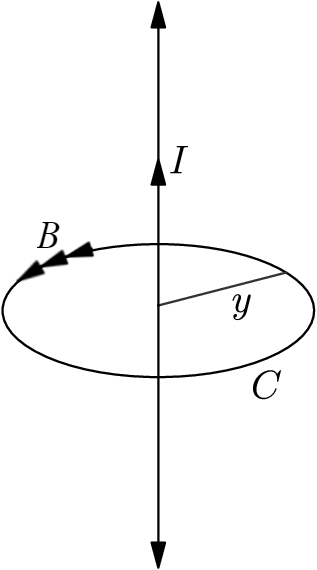
\includegraphics[scale=0.25]{images/em/ampere.png}
\end{center}
Consider the Amperian loop that is a circle centered on the current with radius $y$ passing through the point at which we were calculating the magnetic field. The current through the loop is clearly $I$ because no other currents are in the setup. Usually, we do line integrals around the loop following the right-hand rule (ie. counterclockwise) so since the magnetic field and each displacement around the loop are going in the same direction, the line integral basically evaluates to the circumference times the magnetic field's magnitude. If we substitute into Ampere's Law, we have:
\[
	B \cdot 2\pi y = \mu_0 I
\]
And we can see pretty clearly that we have: 
\[
	B = \frac{\mu_0I}{2\pi y}
\]
just as before. \\
There exist uniform magnetic fields that we haven't explored - the most common one is the field of a solenoid, which is basically a really long coil of wire. We can characterize a solenoid by the number of turns or loops it has, $N$; its length, $L$; and the current through the wire, $I$. 
\begin{center}
	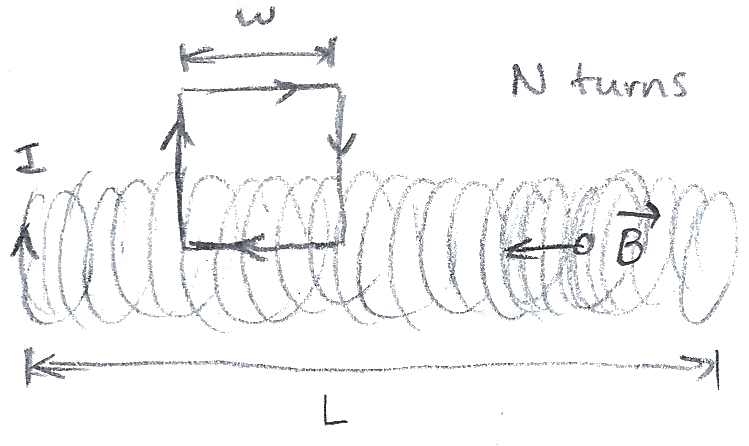
\includegraphics[scale=0.25]{images/em/solenoid.png}
\end{center}
We can use Ampere's Law on a rectangular loop passing through the sides of the solenoid. If the rectangle has width $w$, we can figure out the current passing through the loop:
\[
	\oint_C \vec B \cdot d\vec s = \mu_0 I \frac{N}{L} w
\]
When we integrate around the loop, by symmetry, we know the magnitude of the magnetic field a distance $r$ from the axis of symmetry is all the same. It's also true that the two sides passing through the solenoid will cancel each other out since they're going in different directions. Also, outside of the solenoid, the magnitude of the field is so small that it is effectively zero, especially if the solenoid is really long. Therefore, once we actually evaluate the line integral, we have:
\[
	B(r) w =  \mu_0 I \frac{N}{L} w \quad
	B(r) = \mu_0 I \frac{N}{L}
\]
You might be wondering why we don't have something like Gauss' Law for Magnetism that we can use to calculate magnetic fields. This is because - well, it's not very useful. Similar to electric flux, Gauss' Law uses magnetic flux, which will be discussed at length in the next section - but you can imagine it's similar to electric flux. Gauss' Law for Magnetism states that:
\[
	\oint_S \vec B \cdot \hat n \, dA = 0
\]
This is an interesting result - and we can see that it is true because magnetic field lines form closed loops in space. Because of this, all the field lines must enter and exit the Gaussian surface, so the flux out perfectly cancels the flux in. This means that it's impossible to have some kind of source or sink of the magnetic field - ie. there's no such thing as a magnetic "charge", or monopole, the same way that there is an electric charge (or if there is, we haven't observed it yet). However, it's not terribly useful in calculating the magnetic fields of objects, but it's still important as it implies the non-existence of spherically symmetric magnetic fields. This drastically limits the amount of easily-computable magnetic fields that there are. 
\subsection{Faraday-Lenz's Law and Induction}
We're now going to talk about one of the weirdest things about electricity and magnetism - the concept of induction. First, we have to look at magnetic flux - it's the same thing as electric flux, except for magnetic fields through an area. You can calculate the flux through a flat surface by taking the dot product of the field and the normal vector times the area, and you can break up a curved or weird surface in general into small, infinitesimally small approximately flat surfaces and add up the magnetic flux to find the total:
\[
	\Phi_B = \vec B \cdot \hat n \, A \quad \Phi_B = \int_S \vec B \cdot \hat n \, dA
\] 
It turns out people have a special name for the unit of magnetic flux - it's called a weber (Wb), or a T$\cdot$m$^2$. \\
The magnetic field can be used to generate, or induce, an electric field in a region of space. The Faraday-Lenz Law states that if the magnetic flux is changing with time through some surface bounded by the loop, then an emf is induced in the loop. The rate of change of the magnetic flux is the negative of the emf:
\[
	\oint_C \vec E \cdot d\vec s = \mathscr{E} = -\dv{\Phi_B}{t} = -\dv{}{t} \int_S \vec B \cdot \hat n \, dA
\]
This process is called induction, and in fact, this changing magnetic field generates an electric field that produces this emf. However, the electric field lines here are closed loops and are not like the Coulomb electric fields generated from electric charges and they're non-conservative. \\
Faraday's Law (just the part formulated by Faraday) basically states the magnitude of the emf is equal to the magnitude of the change in the magnetic flux per unit time. However, it's sometimes confusing to figure out which way the emf is going around the loop. Lenz's Law tells us exactly how it's directed - the minus sign in front of the emf indicates that the emf generated opposes the magnetic flux. To be clear, the emf creates a current in the loop, which we know creates its own magnetic field; and Lenz's Law says that this generated magnetic field will try to compensate for the change in the flux and try to stop the change. \\
\begin{center}
	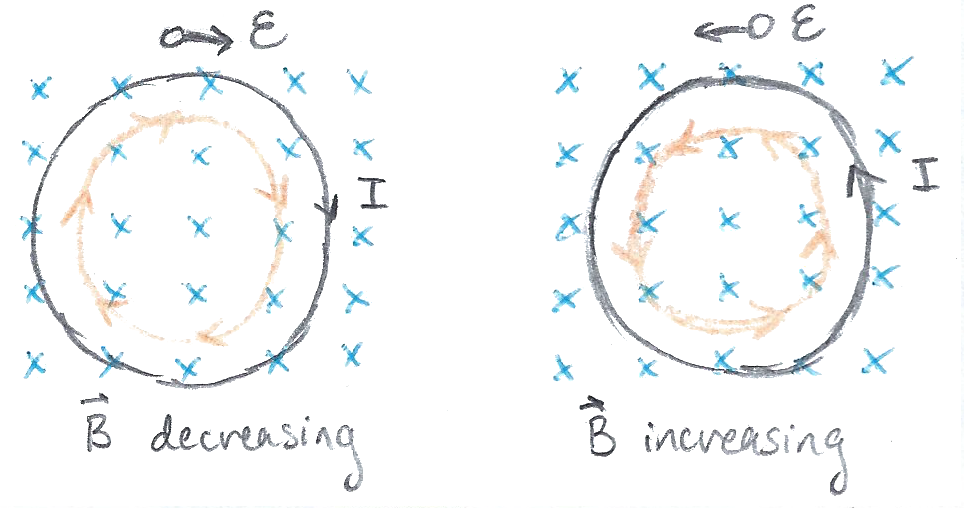
\includegraphics[scale=0.25]{images/em/faraday-lenz.png}
\end{center}
Let's just look at an example. Suppose we have a small circular loop and a magnetic field going into the page and assume the magnitude of the magnetic field is decreasing.\\
Since the magnetic field is decreasing, the emf induced should generate a magnetic field that should increase the magnetic flux. The current around a loop creates a magnetic field according to the right-hand rule - if the fingers curl around in the direction of the current, then the thumb will point in the direction of the magnetic field generated. This means then the magnetic field generated should also point into the page, so the current and emf are directed clockwise around the loop. Similarly, if the magnetic field was increasing, the emf induced should decrease the magnetic flux, which would be achieved if the emf were directed counterclockwise. \\
One of the most common applications of Faraday-Lenz is to a rail gun. Let's consider a metal bar of length $L$ and resistance $R$ sitting on parallel conducting tracks, and the bar can slide back and forth perpendicular to the tracks. There's a battery with emf $\mathscr E$ hooked up to the rails, and a uniform magnetic field $\vec B$ (directed into the page) is present throughout the entire system. Suddenly, the bar is pushed to the right at a velocity $v_0$... and what happens?\\
\begin{center}
	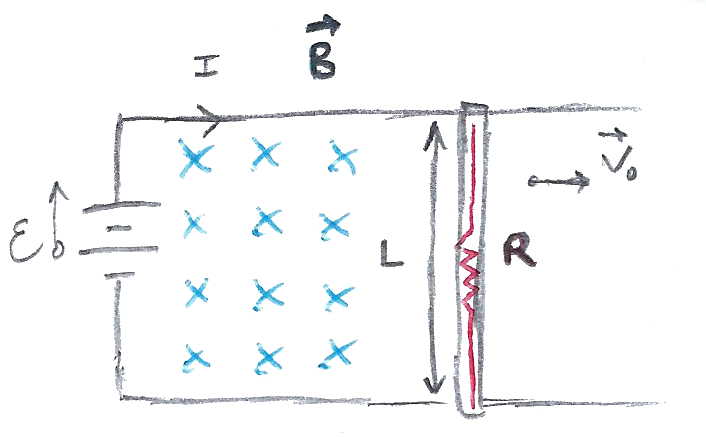
\includegraphics[scale=0.25]{images/em/railgun.png}
\end{center}
Well, let's first just look at the forces on the bar. We could naively say that the force is simply the force on a current that we calculated earlier:
\[
	\vec F = I \vec L \times \vec B 
\]
We know the current is flowing clockwise, so $\vec L$ is directed directly downward, so the resultant force is directed to the right (due to the cross product). This force does non-zero work on the bar because the bar and the force are in the same direction - but this contradicts the fact that forces due to magnetism do not do any work at all! Something is wrong, and it has to do with this analysis of the situation. This formula is only valid if the bar is static and not moving - but once the bar starts to move, other forces are at play. 
The electrons in the bar are both moving rightward with the bar, but also, because of the current, they are also drifting along up the page (as they move opposite to the current due to their negative charge). By the Lorentz Force Law, we can start from scratch and calculate on each electron:
\begin{align*}
	\vec F &= -e(\vec v_D + \vec v_0) \times \vec B\\
	&= -e\vec v_D \times \vec B + (-e) \vec v_0 \times \vec B
\end{align*}
Let's look at these two parts of the term. The first term $-e \vec v_D \times \vec B$ we can recognize as pointing to the right, and from scaling this up by multiplying through by the volume and the density of the electrons, it results in the familiar $I \vec L \times B$ that we know, which does positive work on the bar. \\
On the other hand, the other term $-e \vec v_0 \times \vec B$ is directed down the page, and it pushes all the electrons down the bar. We can see that negative work is done by this force as this magnetic force is exerted on all the electrons traveling down the bar of length $L$. Therefore, the work due to this force is:
\[
	W = -ev_0BL
\]
And as we noted before, the sign is expected to be negative because it needs to cancel the positive work done by the other component of the force. Let's just go one step further and look at the work done per unit charge:
\[
	\mathscr{E}_{ind} = v_0BL
\]
Since we noted that work done by the magnetic force on the electrons in the bar was negative, the work per unit (negative) charge is positive. This work per unit charge is going up the bar, against that exerted by the battery, because negative work is done down the bar. It turns out that this work per unit charge is the induced electromotive force as a result of the changing magnetic flux through the loop formed by the circuit. At least we can see the dimensions are correct through dimensional analysis, but it's not easy to see that this is true. Let's apply Faraday's Law to this situation to see that this is in fact true. \\
In this case, the magnetic flux is increasing not because the field is growing stronger, but because the area is increasing. The area is increasing at a rate of $Lv_0$, so then the rate at which the magnetic flux is changing is:
\[
	\dv{\Phi_B}{t} = BLv_0
\]
The two expressions match in magnitude, but we need to check that the directions of these emfs match. Using Lenz's Law, because the magnetic flux is increasing (and going into the page), the induced emf should create a current that creates a magnetic field going out of the page. This would mean that the current should flow counterclockwise, and so the emf should go counterclockwise, which is consistent with our analysis of the situation using forces. \\
Notice that there's really nothing special about looking at the scenario at $t=0$ - this fact wasn't really ever used, so in general, the emf induced is equal to 
\[
	\mathscr{E} = BLv
\]
where $v$ is the velocity of the bar in the rightward direction at any time. \\
As problems to be solved later, we will look at the current in the bar as a function of time, and the velocity of the bar as a function of time (and note that while the bar shoots off to infinity, it actually eventually reaches a terminal velocity). 
\subsection{Inductance and Circuits Revisited}
With our knowledge of magnetism, we can introduce one last circuit element - the inductor. We have to talk about inductance first, which is a measure of the tendency of a circuit or a conductor (with a closed loop) to induce an emf due to changing currents and has the SI unit of henries (H). Because conductors generate magnetic fields, which are created using current, a changing current will create a changing magnetic field, and therefore a changing magnetic flux. From Faraday-Lenz, we know that a changing magnetic flux in a closed loop will induce an emf in that loop that will act against the change of the magnetic flux. This ratio of the induced emf $\mathscr{E}_{ind}$ to the change in the current per unit time is the inductance $L$, or in other terms:
\[
	\mathscr{E}_{ind} = -L\dv{I}{t}
\]
We can also express the inductance as the ratio of the magnetic flux through a conductor (for loops and coils) to the current through it:
\[
	\Phi_B = LI
\]
This means that 1 H = 1 Wb/A. Furthermore, since the first equation is effectively the time derivative of the second (and an application of Faraday-Lenz) because the derivative of the inductance did not appear, it implies that the inductance $L$ is independent of time. This is true - it turns out the inductance of a conductor is only dependent on the geometry of the conductor, kind of like capacitance is also dependent only on geometry. We can show this is true because the magnetic field is directly proportional to the current, which is also directly proportional to the magnetic flux. \\
Technically speaking, there are two types of inductance - self-inductance and mutual inductance. Self-inductance $L$ is the tendency for a conductor to induce an emf in itself, but mutual inductance $M$ refers to inducing an emf in another conductor (and obeys the same formulas as self-inductance). Most of the time, we will neglect considering the mutual inductance from a conductor to another conductor, because if the current in the first is varying non-linearly, the emf and current produced by the second will create a changing magnetic flux in the first, and soon you have this Russian-nesting-doll type scenario that gets complicated. \\
\begin{center}
	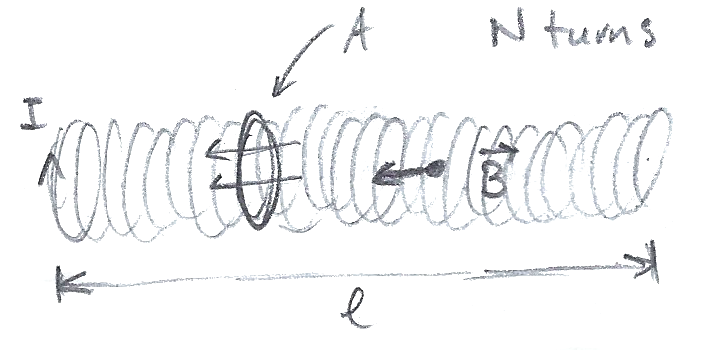
\includegraphics[scale=0.25]{images/em/inductor.png}
\end{center}
As an example, we can look at the self-inductance of a solenoid of $N$ turns with length $l$, cross-sectional area $A$, and current $I$. Remember that the magnetic field of a solenoid is uniform and is:
\[
	B = \mu_0 \frac{N}{l}I
\]
The flux through one turn of the solenoid is the magnetic field times the cross sectional area. However, we have to add up the flux for all the turns, so we have:
\[
	\Phi_B = \mu_0 \frac{N^2A}{l} I
\]
Therefore, the self-inductance $L$ is
\[
	L = \mu_0 \frac{N^2A}{l}
\]
Inductors are circuit elements that have non-negligible self-inductance and as stated earlier, create a resistant emf of magnitude $L\dv{I}{t}$. Work must be done on the inductor in order to get the desired current to flow through the inductor. If we multiply through by the current, we get the rate at which work is done. For a time interval $dt$, the work done on the inductor is then:
\[
	dW = L\dv{I}{t} \cdot I \, dt = LI\, dI
\]
If we increase the current from $0$ to $I$, the work done at the end of the process will be: 
\[
	W = \int_0^I LI\, dI = \frac{1}{2}LI^2
\]
This energy is actually stored in the magnetic field of the inductor, with density per unit volume
\[
	u_B = \frac{1}{2} \frac{B^2}{\mu_0}
\]
As for the case with electric fields, it's difficult to show this is true in the general case, but we can certainly confirm it for our solenoid example. If we plug in our value of the inductance of a solenoid, we can get the energy stored to be:
\[
	U \mu_0 \frac{N^2AI^2}{2l}
\]
The density per unit volume is:
\[
	u_B = \frac{1}{2} \left( \mu_0 \frac{N}{l}I\right)^2 \frac{1}{\mu_0} = \frac{\mu_0 N^2 I^2}{2l^2}
\]
If we multiply through by the volume $Al$, we do get the stored energy in the solenoid, which confirms this formula for this case.\\
In circuits, inductors follow the same rules as resistors because of their similar dependency on the current of the circuit. For two inductors in series with inductances $L_1$ and $L_2$, we have that their effective inductance is 
\[
	L = L_1 + L_2
\]
For the same two inductors in parallel, we have that their effective inductance $L$ is related to these inductances by
\[
	\frac{1}{L} = \frac{1}{L_1} + \frac{1}{L_2}
\]
Again, this is generalizable to larger numbers of inductors. Using these formulas, we can now treat any number of inductors in series or in parallel as essentially one inductor. \\
We are now going to revisit circuitry for real and look at circuits in conjunction with resistors and capacitors. First, let's look at a single-loop LR circuit, with a battery, inductor and a resistor.
\begin{center}
	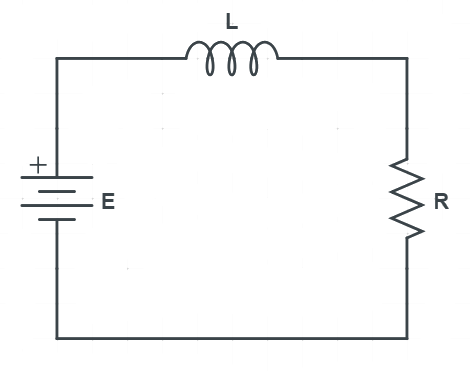
\includegraphics[scale=0.25]{images/em/LR-circuit.png}
\end{center}
Letting the battery have emf $\mathscr{E}$, the resistor a resistance $R$, and the inductor an inductance $L$, we use Kirchhoff's Voltage Law:
\[
	\mathscr{E} - IR - L\dv{I}{t} = 0
\]
We can now rearrange and integrate from time $t=0$ to arbitrary time $t$ just like we did before with an RC circuit, assuming the current at time $t=0$ is zero:\\
\[
	L\dv{I}{t} = \mathscr{E} - IR
\]
\[
	\frac{L}{\mathscr{E} - IR} \dv{I}{t}  = 1
\]
\[
	\int_0^t \frac{L}{\mathscr{E} - IR} \dv{I}{t} \, dt =  \int_0^t 1 \, dt
\]
\[
	-\frac{L}{R} \ln\left(\frac{\mathscr{E} - I(t)R}{\mathscr{E}}\right) = t
\]
\[
	\mathscr{E} - I(t)R = \mathscr{E}e^{-\frac{R}{L}t}
\]
\[
	I(t) = \frac{\mathscr{E}}{R}(1 - e^{-\frac{R}{L}t})
\]
A few remarks: at time $t=0$ the current is $\frac{\mathscr{E}}{R}$, and the inductor doesn't influence the current, so it behaves like a normal wire. However, as $t \to \infty$, the current approaches $0$. This is because inductors take the energy out of the circuit and stores it inside its magnetic field, just like capacitors. However, the increasing magnetic field in the inductor creates an emf against the emf from the battery and eventually stops the flow of current through the inductor, acting like a broken wire. This behavior is general for all inductors. Similar to RC circuits, LR circuits have a time constant $\tau = \frac{L}{R}$, also measuring the speed at which energy is stored into the inductor. From here, we can see that a henry per ohm is also a second - which is a weird combination of units to equal a second, but it works and you can check if you call BS. \\
Moving on to LC circuits - usually, we're only going to consider the starting state to be a fully charged capacitor with capacitance $C$, and an inductor with no current through it with inductance $L$. (You'll see why we've omitted the battery on purpose in this case.) 
\begin{center}
	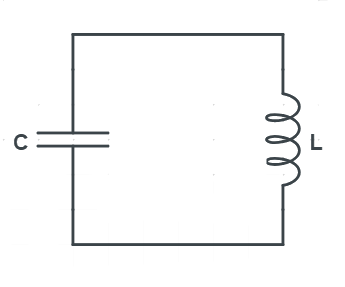
\includegraphics[scale=0.25]{images/em/LC-circuit.png}
\end{center}
Since the capacitor is discharging, it provides a positive emf, while the inductor takes out energy and stores it in its magnetic field. We can use Kirchhoff's Voltage Law:
\[
	\frac{Q}{C} - L \dv{I}{t} = 0
\]
If we note that in this case $I = -\dv{Q}{t}$ (since the charge on the capacitor is decreasing, and the current is always positive) we can rearrange to obtain:
\[
	\frac{Q}{LC} = \dv{I}{t} = -\dv{}{t} \dv{Q}{t} = -\ddv{Q}{t}
\]
This means the second time-derivative of charge is proportional to the charge - which is precisely the differential equation for a simple harmonic oscillator! In this case, the resonant frequency of the circuit is $\omega = \frac{1}{\sqrt{LC}}$. This means that if we consider the charge at time $t=0$ to be $Q_0 > 0$, we can express the charge on the capacitor plates as a function of time to be
\[
	Q(t) = Q_0\cos\left(\frac{1}{\sqrt{LC}}t\right)
\]
where negative values of charge indicate the negative and positive plates of the capacitor have been flipped. Once we take the derivative, we get the current in the circuit at any time to be:
\[
	I(t) = -\frac{Q_0}{\sqrt{LC}}\sin\left(\frac{1}{\sqrt{LC}}t\right)
\]
where negative values of the current indicate the current has changed direction. Because there is no resistance in the circuit, we can see that the stored energy in the circuit is conserved at any given point. Recall that the stored energy in a capacitor is $\frac{1}{2}\frac{Q^2}{C}$, so at the beginning the energy stored is:
\[
	E_{0} = \frac{1}{2}\frac{Q_0^2}{C}
\]
At any given time $t$ the stored energy in the capacitor is:
\[
	E_C = \frac{1}{2}\frac{Q(t)^2}{C} = \frac{1}{2}\frac{Q_0^2 \cos^2\left(\frac{1}{\sqrt{LC}}t\right)}{C}
\]
In the inductor, we can find the energy in the inductor to be:
\[
	E_L = \frac{1}{2}LI^2 = \frac{1}{2}L\left(-\frac{Q_0}{\sqrt{LC}}\sin\left(\frac{1}{\sqrt{LC}}t\right) \right)^2
\]
We can sum this up to find the total energy in the system:
\begin{align*}
	E^{tot} &= \frac{1}{2}\frac{Q_0^2 \cos^2\left(\frac{1}{\sqrt{LC}}t\right)}{C} + \frac{1}{2}L\left(-\frac{Q_0}{\sqrt{LC}}\sin\left(\frac{1}{\sqrt{LC}}t\right) \right)^2 \\
	&= \frac{Q_0^2 \cos^2\left(\frac{1}{\sqrt{LC}}t\right)}{2C} + L\frac{Q_0^2\sin^2\left(\frac{1}{\sqrt{LC}}t\right)}{2LC}\\
	&= \frac{Q_0^2}{2C}\left( \cos^2\left(\frac{1}{\sqrt{LC}}t\right) + \sin^2\left(\frac{1}{\sqrt{LC}}t\right)\right) \\
	&= \frac{Q_0^2}{2C}
\end{align*}
Our results agree, as expected. The time constant for the $LC$ circuit, that is, $\tau = \sqrt{LC}$, shows up everywhere in these calculations, especially because it shows up as the frequency of the circuit. This means the period of the circuit is $T = \frac{2\pi}{\omega} = 2\pi \sqrt{LC}$. (Also, we get one last interesting combination for time - an ohm-henry is a second squared.)\\
Inductors are an important part of circuits that you should know how to handle, and while in general all circuits have inductance, capacitance, and resistance to some degree that you should know how to handle, circuits with all of these explicit elements in them aren't important to AP Physics (because the model for these equations is pretty difficult, but in short, the function for current models dampened oscillations, and looks like a sine wave except as $t \to \infty$ the current goes to zero). Circuits are a difficult concept to master, and it takes a lot of practice and intuition to be able to quickly build the correct quantitative model of the situation.
\subsection{Summary and Problems}
Magnetism is an extremely broad topic - we first looked at how magnetic fields are generated from moving currents and how they exert a force on electric charges. We then looked at magnetic induction and Faraday's Law, where a changing magnetic flux induced an electric field and emf in a loop. Finally, we looked a bit more into the inductance of loops and inductors, the final circuit element involving a magnetic field's effect on creating a voltage drop in the circuit. \\

\noindent \textbf{Problems:}\\
1. (1 $\bigstar$, $\spadesuit$) A current-carrying wire is bent into a closed semicircular loop of radius R that lies in the $xy$-plane. The wire is in a uniform magnetic field that is in the $+z$-direction. Verify that the force acting on the loop is zero. \\
2. (3 $\bigstar$) A simple gaussmeter for measuring horizontal magnetic fields consists of a stiff wire of length $L$ that hangs from a conducting pivot so that its free end makes contact with a pool of mercury in a dish below. The mercury provides an electrical contact without constraining the movement of the wire. The wire has a mass of $m$ and conducts a current downward. If the horizontal magnetic field is $B$ and the current is $I$, show that the equilibrium angular displacement of the wire from vertical is $\theta = \arcsin  \left(\frac{ILB}{mg}\right)$.\\
3. (3 $\bigstar$) A uniform magnetic field $B$ is perpendicular to the base of a hemisphere of radius $R$. Show that the magnetic flux (in terms of $B$ and $R$) through the spherical surface of the hemisphere is $\pi R^2 B$. \\
4. (2 $\bigstar$) A beam of particles with velocity $\vec v$ enters a region that has a uniform magnetic field $\vec B$ in the $+x$-direction. Show that when the velocity of the particle is again in the same direction as it was when the particle entered the field, the $x$-component of the displacement of one of the particles is $\frac{2\pi m}{qB}v \cos \theta$ where $\theta$ is the angle between $\vec v$ and $\vec B$.\\
5. (3 $\bigstar$, $\spadesuit$) Revisit the railgun setup. Consider a metal bar of mass $m$, length $L$, and resistance $R$ sitting on parallel conducting tracks, and the bar can slide back and forth perpendicular to the tracks. A battery with emf $\mathscr E$ is hooked up to the rails, and a uniform magnetic field $\vec B$ goes through the entire region perpendicular to the plane of the tracks. a) If the bar starts from rest, show that the terminal velocity of the bar is $\frac{\mathscr{E}}{BL}$ and that the velocity of the bar as a function of time is $v(t) = \frac{\mathscr{E}}{BL}(1 - e^{-\frac{B^2L^2}{mR}t})$. b) Show that the current in the bar starts at $I = \frac{\mathscr{E}}{R}$, and the current in the bar can be modeled as $I(t) = \frac{\mathscr{E}}{R}e^{-\frac{B^2L^2}{mR}t}$.\\
6. (3 $\bigstar$, $\spadesuit$) Consider a point $P$ on the perpendicular bisector of a wire segment of length $2a$ carrying a current $I$, a distance $R$ away from the midpoint of the segment. a) Show that the magnetic field strength at $P$ is $B = \frac{\mu_0Ia}{2\pi R\sqrt{a^2 + R^2}}$ b) Use your result from part a) to show that the magnetic field strength at the center of a regular polygon of N sides is $\frac{\mu_0IN}{2\pi R} \sin \left(\frac{\pi}{N}\right)$. c) Show that when $N$ is very large, your result approaches that for the magnetic field strength at the center of a circle.\\
7. (2 $\bigstar$) A mass spectrometer uses a velocity selector to guarantee that all the ions enter the main chamber with the same speed. A uniform magnetic field with magnitude $B$ covers the region of the velocity selector and the chamber of the mass spectrometer. In this mass spectrometer, ions with charge $+e$ with different masses will move in a semicircle before colliding with the back wall of the chamber. The spectrometer is designed so that if two ions have a mass difference of $\Delta m$, they will hit the back wall separated by a distance $\Delta x$. Show that the magnitude of the electric field in the velocity selector needs to be $E = \frac{eB^2\Delta x}{2\Delta m}$ for this to work. \\
8. (1 $\bigstar$) The Hall experiment showed that the fundamental charges that we observed around us had a negative sign. Consider a box of height $h$, cross-sectional area $A$, and a uniform magnetic field running parallel to the bottom plane of the box $\vec B$. a) Suppose we inject charged particles into the box moving at a velocity $v$. Show that at equilibrium, the potential difference between the top and bottom of the box is $vhB$. b) Suppose that if we measure the potential difference between the top and bottom of the box to be positive. Show that this is the case if the charges are negative, and the opposite is true if the charges are positive. \\
9. (2 $\bigstar$) A long cylindrical shell has an inner radius $a$ and an outer radius $b$ and carries a current $I$ parallel to the central axis. Assume that within the material of the shell the current density is uniformly distributed. Show that the magnitude of the magnetic field is, if $r$ represents the distance from the central axis, that a) $B = 0$ if $r < a$, b) $B = \frac{\mu_0 I}{2\pi r}\frac{r^2 - a^2}{b^2 - a^2}$ if $b > r > a$, c) $B = \frac{\mu_0 I}{2 \pi r}$ if $r > b$.\\
10. (2 $\bigstar$) At some instant in an oscillating LC circuit, $k$\% of the total energy is stored in the magnetic field of the inductor. a) Show that the multiple of the maximum charge $Q_{max}$ that is on the capacitor is $\sqrt{1-\frac{k}{100}}Q_{max}$ b) Show that the multiple of the maximum current $I_{max}$ that is in the inductor is $\frac{\sqrt{k}}{10}I_{max}$.\\
11. (3 $\bigstar$, $\spadesuit$) In the circuit below, the switch is closed to point $A$ at time $t=0$, with zero initial charge on the capacitor. When the switch is closed, the current is $I_0$. The switch is thrown to point $B$ when the current is $\frac{I_0}{3}$. Show that the maximum current in the inductor after the switch was thrown to point $B$ is $\frac{2}{3} \mathscr{E} \sqrt{\frac{C}{L}}$.
\begin{center}
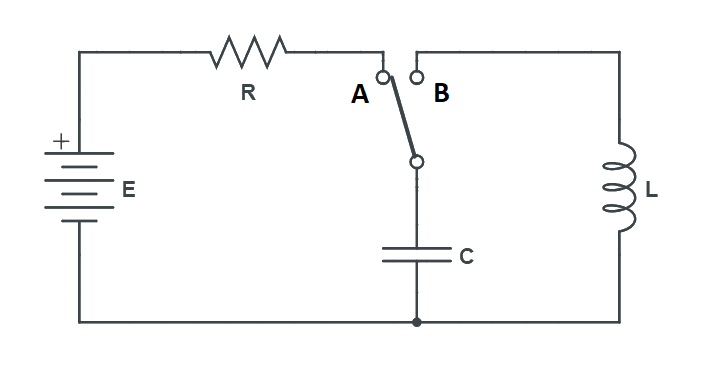
\includegraphics[scale=0.42]{images/em/switchingcircuit.png}
\end{center}
12. (4 $\bigstar$, $\spadesuit$) In the circuit above, the switch is closed to point $A$ at time $t=0$, with zero initial charge on the capacitor. The switch is thrown to point $B$ after a time $\Delta t$. When the energies in the capacitor and in the inductor are equal, show that the current in the inductor is $\mathscr{E}(1- e^{-\frac{t}{RC}})\sqrt{\frac{C}{2L}}$. \\
13. (4 $\bigstar$, $\spadesuit$) A rectangular loop of wire that has width $w$, length $l$, and lies in the vertical plane which is perpendicular to a region that has a uniform magnetic field. The magnitude of the uniform magnetic field is $B$ and the direction of the magnetic field is into the page. The portion of the loop not in the magnetic field has length $y$. The resistance of the loop is $R$ and its mass is
$m$. The loop is released from rest at $t = 0$. (Let down be the $+y$-direction.) Show that the speed of the loop $v$ as a function of time is $v(t) = \frac{mgR}{B^2w^2}(1- e^{-\frac{B^2w^2}{mR}t})$.\\
14. (3 $\bigstar$) A conducting rod of length $l$ rotates at constant angular speed $\omega$ about one end, in a plane perpendicular to a uniform magnetic field $B$. Compute the flux $\Phi_m$ through the area swept out during a time $\Delta t$, and show that the motional emf in the rod is given by $\frac{1}{2}\omega Bl^2$.

\pagebreak

\section{Maxwell's Equations}
AP Physics C doesn't require you to know Maxwell's equations - however, you already know them from studying the behaviors of electric and magnetic fields, so I feel like it's worth at least looking at them. Maxwell's equations are four equations that govern the behavior of all electric and magnetic fields - they are Gauss' Law for Electric Fields, Gauss' Law for Magnetic Fields, Faraday-Lenz's Law, and Ampere's Law. 
\subsection{The Error and the Fix}
We would like Maxwell's equations to describe electromagnetic fields regardless of their configuration in space. Currently, however, there's an issue with Ampere's Law as we know it, and we're going to look at why it's wrong as well as what we need to add to fix it. \\
\begin{center}
	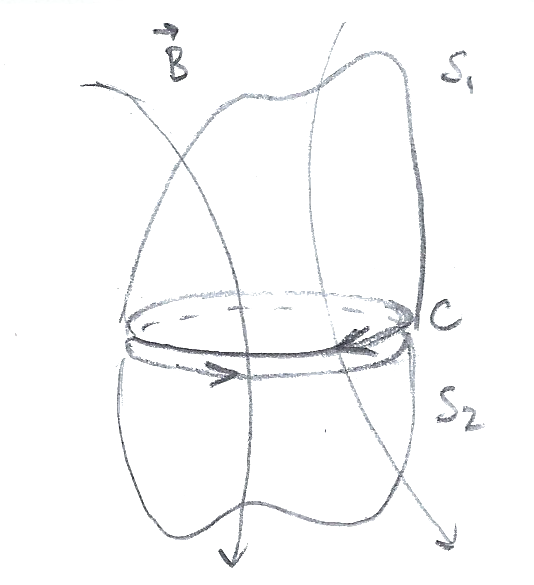
\includegraphics[scale=0.25]{images/em/faraday-surface.png}
\end{center}
First, let's look at how Faraday's Law is independent of the surface of which one calculates the flux. Consider a loop $C$ in space, and a surface $S_1$ bounded by the loop. We can apply the Faraday-Lenz Law:
\[
	\oint_C \vec E \cdot d\vec s = - \dv{}{t} \int_{S_1} \vec B \cdot \hat n \, dA
\]
Usually, we take loop integrals in the counterclockwise direction around the loop, but we can also consider a surface $S_2$ on the opposite side of the loop from $S_1$, from which we can apply Faraday-Lenz by integrating in the clockwise direction:
\[
	\oint_C \vec E \cdot d(-\vec s) = - \dv{}{t} \int_{S_2} \vec B \cdot \hat n \, dA
\]
Now, let's add these together. Notice the left side goes to 0, but when we combine the two flux integrals over surfaces $S_1$ and $S_2$, they form a closed surface. Because we assume Gauss' Law for Magnetism is true, this flux integral is 0!
\[
  - \dv{}{t} \int_{S_1} \vec B \cdot \hat n \, dA  - \dv{}{t} \int_{S_2} \vec B \cdot \hat n \, dA  = - \dv{}{t} \oint_{S_1+S_2} \vec B \cdot \hat n\, dA = -\dv{}{t} 0 = 0
\]
Because we haven't explicitly chosen a surface to take the magnetic flux through, Faraday-Lenz is independent upon the choice of the surface for the magnetic flux. However, let's look at Ampere's Law, which is not general for all cases (yet). \\
\begin{center}
	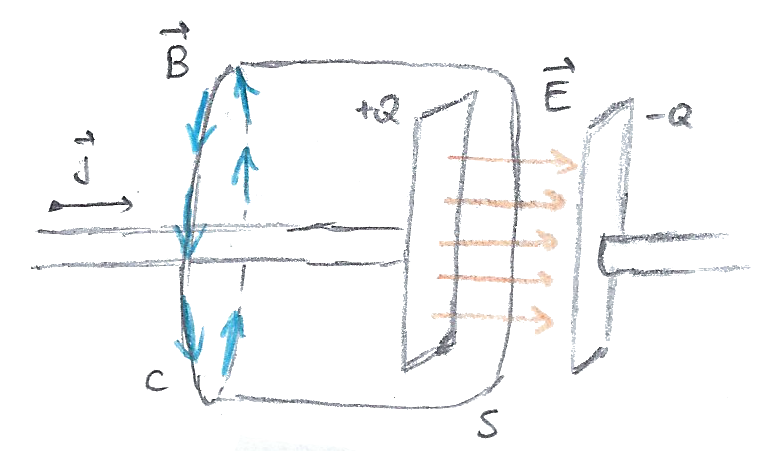
\includegraphics[scale=0.25]{images/em/ampere-capacitor.png}
\end{center}
Consider a straight wire connected to a parallel-plate capacitor:\\
We can apply Ampere's Law to the magnetic field in a circular loop $C$ with radius $r$ around the current running through the wire, and we know from the Magnetism unit that the magnetic field is non-zero. If we just consider the surface $S$ in the same plane as the loop, remember that we can derive the magnitude of the magnetic field:
\[
	\oint_C \vec B \cdot d\vec s = \mu_0 \int_S \vec j \cdot \hat n \, dA = \mu_0 I \rightarrow B \, 2\pi r = \mu_0 I \rightarrow B = \frac{\mu_0I}{2\pi r}
\]
What if we consider a surface $S$ that passes between the plates of the capacitor? No current runs between the plates of a capacitor, so then the right hand side of Ampere's Law goes to zero. However, the left-hand side of Ampere's Law we just saw to be nonzero! Something has gone horribly wrong...\\
Remember that the current charges the plates of the capacitor over time, creating an electric field in the capacitor. Maybe we should look at the electric field as it changes with time to see how we can still obtain the correct expression for the current in the wire from the electric field. Remember the electric field in a capacitor has magnitude $\frac{\sigma}{\epsilon_0}$, with $\sigma = \frac{Q}{A}$ as the charge density per unit area:
\[
	E = \frac{\sigma}{\epsilon_0} = \frac{Q}{A\epsilon_0}
\]
We can actually find the electric flux through the surface $S$! Since the electric field only penetrates through an area of $A$, we can find the electric flux $\Phi_E$ to be:
\[
	\Phi_E = EA = \frac{Q}{\epsilon_0}
\]
To find the current, we can isolate the charge, and take a time-derivative:
\[
	Q = \epsilon_0 EA = \epsilon_0 \Phi_E \rightarrow I = \dv{Q}{t} = \epsilon_0 \dv{\Phi_E}{t} = \epsilon_0 \dv{}{t} \int_S \vec E \cdot \hat n \, dA
\]
Notice that we now have a new expression for the current. If we just plugged this back into Ampere's Law, we could fix the problem! It turns out James Clark Maxwell figured he could do this, so we can write Ampere's Law (with Maxwell's correction):
\[
	\oint_C \vec B \cdot d\vec s = \mu_0 \left(\int_S \vec j \cdot \hat n \, dA + \epsilon_0  \dv{}{t} \int_S \vec E \cdot \hat n \, dA\right)
\]
This is the correct form of Ampere's Law. This added term is called the displacement current - even though it's not actually a current, it compensates so that it considers changing electric flux as "current" for surfaces that don't have any current through them. With this, we can show that Ampere-Maxwell's Law (what we're going to call the corrected form of Ampere's Law) is true for any surface, using the same tactic we used earlier for Faraday's Law. \\
\begin{center}
	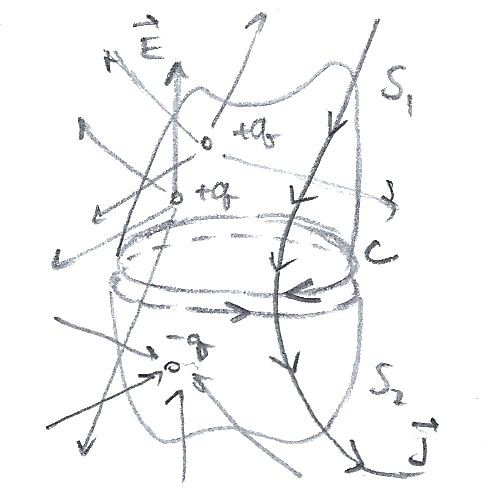
\includegraphics[scale=0.25]{images/em/ampere-surface.png}
\end{center}
Consider two surfaces $S_1$ and $S_2$ both bounded by a loop but on opposite sides of the loop. We can apply Ampere-Maxwell, but integrate both ways around the loop, attaining expressions pertaining to $S_1$ and $S_2$:
\[
	\oint_C \vec B \cdot d\vec s = \mu_0 \int_{S_1} \left(\vec j + \epsilon_0  \dv{}{t}\vec E\right) \cdot \hat n \, dA
\]	
\[
	\oint_C \vec B \cdot d(-\vec s) = \mu_0 \int_{S_2} \left(\vec j + \epsilon_0  \dv{}{t}\vec E\right) \cdot \hat n \, dA
\]
If we add them together, and consider the union of surfaces $S_1$ and $S_2$ into a single closed surface, we can simplify greatly:
\[
	\mu_0 \oint_{S_1+S_2} \vec j \cdot \hat n \, dA + \mu_0 \epsilon_0 \dv{}{t} \oint_{S_1+S_2} \vec E \cdot \hat n \, dA = 0
\]
We can apply Gauss' Law to the second term, and substitute in current $I_{out}$ for the first term:
\[
	\mu_0 I_{out} + \mu_0 \dv{Q_{inside}}{t} = 0
\]
In order for Ampere-Maxwell to be correct for any surface, if a net current flows out of a region, the charge inside the region must be changing at the same rate. This basically means that charge should be locally conserved, where the only way the charge inside a region can change is if a current explicitly carry it outside of the region. Local conservation of charge is actually a stronger statement than the conservation of charge, which only states that charge can neither be created nor destroyed. We actually just accept this to be true as a fundamental fact of the universe. \\
Because we know that charge is locally conserved, if we look back at the Lorentz Force Law:
\[
	\vec F = \dv{\vec P}{t} = q\vec E + q \vec v \times \vec B
\]
we can note that if charge is locally conserved, so should linear momentum be locally conserved - and for that matter, so should angular momentum and energy, the other two conserved quantities we discussed in mechanics. These three quantities can only change in a system if some form of their time derivatives, being force, torque, or power, change them over time. It seems like common sense, but we never said that there couldn't be a scenario where momentum or energy could just teleport from place to place before this point.\\
Regardless, we now have seen that Maxwell's equations now do apply in every scenario - and we can start to look at their applications in the next section, beyond how they describe everything that we know about electricity and magnetism.
\subsection{The Equations}
Just for the record, let's just state Maxwell's Equations explicitly, where $\rho$ is the density of charge per unit volume (being integrated over a volume) and $\vec j$ is the current density per unit area:
\begin{mdframed}[frametitle=Gauss' Law for Electric Fields]
	$$\oint_S \vec E \cdot \hat n \, dA = \frac{1}{\epsilon_0} \int_V \rho \, dV$$
\end{mdframed}
\begin{mdframed}[frametitle=Gauss' Law for Magnetic Fields]
	$$\oint_S \vec B \cdot \hat n \, dA = 0$$
\end{mdframed}
\begin{mdframed}[frametitle=Faraday-Lenz's Law of Induction]
	$$\oint_S \vec E \cdot d\vec s = -\dv{}{t} \int_S \vec B \cdot \hat n \, dA$$
\end{mdframed}
\begin{mdframed}[frametitle=Ampere-Maxwell's Circuital Law]
	$$\oint_S \vec B \cdot d\vec s = \mu_0 \int_S \left(\vec j + \epsilon_0  \dv{}{t}\vec E\right) \cdot \hat n \, dA$$
\end{mdframed}
Notice that how because of Faraday-Lenz's Law, a changing magnetic field induces an electric field, and because of Ampere-Maxwell's Law, a changing electric field also can create a magnetic field. This begs the question - are there such things as electric and magnetic fields that are self-sustaining? As in, is it possible to have an electric and magnetic field that keep creating more electric and magnetic fields to infinity? 
\begin{center}
	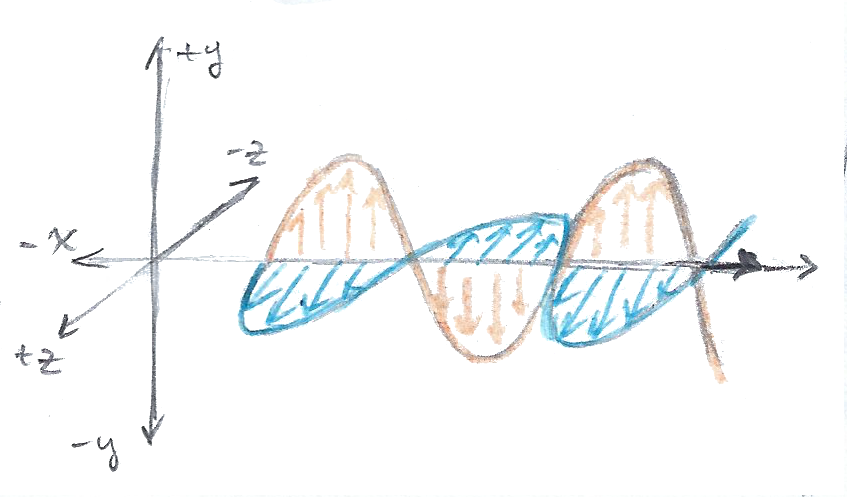
\includegraphics[scale=0.25]{images/em/em-waves.png}
\end{center}
The answer is yes, actually. If just consider free space, where there's no charge and no current, we can create a traveling wave of electric and magnetic fields that sustain each other. It can be shown that this is true and that the speed of this wave $c$ is
\[
	c = \frac{1}{\sqrt{\mu_0\epsilon_0}} = \frac{1}{\sqrt{1.257 \cdot 10^{-6} \, \text{H/m} \cdot 8.854 \cdot 10^{-12} \, \text{F/m}}} = 2.997 \cdot 10^{8} \, \text{m/s}
\]
You might recognize this as the speed of light $c$ in a vacuum - that's because it is. When Maxwell derived this result, he guessed that light itself was simply an electromagnetic wave, and this claim has been tested extensively and is accepted as true. \\

\section*{Electricity and Magnetism Highlights}
\addcontentsline{toc}{section}{\protect\numberline{}Electricity and Magnetism Highlights}
Some of my personal favorite electricity and magnetism problems. These are hard problems, but I strongly encourage you to give most of these a try (except problem 1), because they're good problems. If you feel like you've attempted a problem several times and come up with an incorrect answer, I'd be happy to discuss these with you and go over them.\\
\textbf{Problems:}\\
1. (?? $\bigstar$) Find as many mistakes/inaccuracies as you can in the Electricity and Magnetism section. \\
2. (3 $\bigstar$) A uniformly charged nonconducting solid sphere of radius $a$ has its center at the origin and has a uniform volume charge density of $\rho$. Material is removed from the sphere leaving a spherical cavity that has a radius $r < \frac{a}{2}$ and its center at $x=b$ ($b< \frac{a}{2}$) on the $x$-axis. Show that the electric field inside the cavity is uniform, directed in the $+x$-direction, and has magnitude $\frac{\rho b}{3\epsilon_0}$. \\
3. (3 $\bigstar$, $\spadesuit$) A non-conducting disk has radius $R$, carries a uniform surface charge density $\sigma$, and rotates with angular speed $\omega$. a) Consider an annular strip that has a radius $r$, a width $dr$, and a charge $dq$. Show that the current $dI$ produced by this rotating strip is given by $\sigma \omega r\, dr$. b) Use your result from part a) to show that the magnetic field strength at the center of the disk is given by the expression $B = \frac{1}{2} \mu_0 \sigma \omega R$. c) Use part a) again to show that the magnetic field strength at a point on the central axis of the disk a distance $z$ from its center is $B = \frac{1}{2} \mu_0 \sigma \omega \left(\frac{R^2 + 2z^2}{\sqrt{R^2 + z^2}} - 2z\right)$.\\
4. (4 $\bigstar$) A wooden cylinder with mass $m$, radius $R$, and length $L$ has $N$ turns of wire wrapped around it longitudinally so that the plane of the wire coil contains the long central axis of the cylinder. The cylinder is released on a plane inclined at an angle $\theta$ to the horizontal, with the plane of the coil parallel to the inclined plane. If there is a vertical uniform magnetic field of magnitude $B$, show that the least current $I$ through the coil that keeps the cylinder from rolling down the plane is $\frac{mg}{2NLB}$.\\
5. (5 $\bigstar$, $\spadesuit$) In the circuit shown in the figure below, switch $S$ has been open for a long time. At time $t = 0$ the switch is then closed.
\begin{center}
	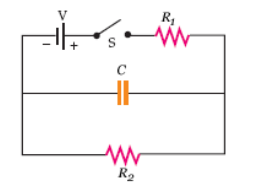
\includegraphics[scale=1]{images/em/RC-problem3.png}
\end{center}
Show that the charge on the capacitor in the steady state is $Q = \frac{\mathscr{E}CR_2}{R_1+R_2}$, and that the charge of the capacitor as a function of time is $\frac{\mathscr{E}CR_2}{R_1+R_2}(1- e^{-\frac{t}{CR_1R_2/(R_1+R_2)}})$.\\
6. (5 $\bigstar$, $\spadesuit$) Consider the circuit shown in the figure where the inductor has negligible
internal resistance and the switch S has been open for a long time. The switch is then closed at time $t=0$.
\begin{center}
	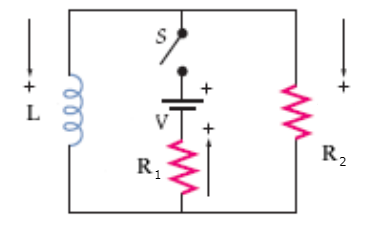
\includegraphics[scale=0.5]{images/em/LR-problem1.png}
\end{center}
Show that the current in the resistor $R_2$ approaches zero in the steady state, and that the current in this resistor can be modeled as $I_2 = \frac{\mathscr{E}}{R_1+R_2}e^{-t(R_1+R_2)/LR_1R_2}$.\\
7. (4 $\bigstar$, $\spadesuit$) A long straight conducting wire with radius $R$ carries a non-uniform current density of magnitude $j(r) = j_0\frac{r}{R}$, where $j_0$ is a positive constant and $r$ is the distance from the axis of symmetry of the wire. This variability in current density is achieved by constructing the wire from a material with variable conductivity $\sigma(r) = \sigma_0 \frac{r}{R}$, where $\sigma_0$ is a positive constant. Let $I$ be the total current in the wire. a) Show that $j_0 = \frac{3I}{2\pi R^2}$. b) Show that if $r>R$, the magnitude of the magnetic field is $B = \frac{\mu_0 I}{2\pi r}$, and if $r < R$, the magnitude of the magnetic field is $B = \frac{\mu_0 I r^2}{2\pi R^3}$. c) Show that the resistance of such a wire with length $L$ is $R = \frac{3L}{\sigma_02\pi R^2}$.\\
8. (4 $\bigstar$, $\spadesuit$) One final railgun problem. A rigid metal bar of length $L$ and mass $m$ slides on two fixed parallel horizontal conducting rods. The bar slides with negligible air resistance and friction. The bar and rods have negligible resistance and form a complete circuit with a sizable resistor of resistance $R$. The system is immersed in a uniform vertical magnetic field of strength $B$. Starting from rest at time $t=0$, the bar is pulled horizontally away from the resistor by an applied constant horizontal force of magnitude $F_0$. Once the bar is in motion, an induced current flows in the bar, and after some time the bar nears a terminal speed $v_T$. a) Show that the terminal speed $v_T = \frac{F_0R}{L^2B^2}$. b) Show that the time it takes for the speed of the bar to reach 3/5 of its terminal speed is $t = \frac{mR}{L^2B^2} \ln \frac{5}{2}$.

\pagebreak


\part{Thermodynamics}
\section{Mathematics Excursion II: Multivariable Calculus}

The A Team employs a relatively frequent use of multivariable calculus in its study of physics. This first lecture is intended to offer the necessary mathematical knowledge about multivariable calculus needed to follow the majority of A Team lectures. New mathematical techniques will be introduced as necessary preceding new topics. 

Assume we are strictly working over the real numbers unless otherwise stated. 
%Notational disclaimer: whenever discussing purely mathematical examples, we will use notation most commonly used by mathematicians -- otherwise, we will use a physicist's notation. 

\subsection{Analyzing Functions of More Than One Variable}
The techniques discussed here generalize to functions of arbitrarily many variables, but for ease of visualization we will limit ourselves to functions of two variables. 

Before we define the multivariable concept of a derivative, it's first appropriate to discuss what limits look like in multiple variables. To do this, we'll intuitively discuss what the rigorous definition of a limit looks like in one-dimensional BC Calculus, and then build from there. 

Recall the following word hash: 
\begin{theorem}[Limit Definition]
The \textit{limit} of the function $f$ as it approaches $a$ is said to be the constant $L$ if for every $\eps > 0$, there exists some $\delta$ such that if $0 < |x-a| < \delta$, $|f(x) - L| < \eps$. 
\end{theorem}

Let's unpack what this is really saying. Suppose we have some function $f(x)$ and we're examining the neighborhood around $x=a$, and the neighborhood around $f(x) = L$. To give these neighborhoods a definite size, say we're only looking a distance of up to $\delta$ around $x=a$ and $\eps$ around $f(x) = L$. If we can shrink or grow $\eps$ at will -- specifically, given that we can make $\eps$ arbitrarily small, if we can always find points on the function (within some $\delta$ away) that encompass those points, the function tends to the limit $L$ as $x$ is said to approach $a$. Notice that the absolute value is important on $|x-a|$, in the sense that this must approach the same value on both sides of $x = a$ -- and obviously, if it doesn't, the limit $L$ cannot take on two different values simultaneously, so it cannot exist. 

This perspective can be generalized somewhat to multivariate functions. Suppose we have a function of two variables, $f(x,y)$, and we are examining the neighborhood around $f(x, y) = L$ and $(x, y) = (a, b)$. In this case, our neighborhood in our range space will be $\eps$ around $f(x,y) = L$, and the neighborhood in our domain space will be a disk of radius $\delta$ around $(a, b)$. As we shrink $\eps$, we must always have some disk of radius $\delta$ whose outputs are contained in $\eps$ above and below $L$. Notice that as we approach the point $(a, b)$, we must pass through every single possible disk of radius $\delta$ corresponding to some $\eps$. So, if while traversing different two paths to $(a, b)$ we approach different values, the limit cannot exist. In particular, we must have that \textbf{all} paths approaching $(a, b)$ must obtain this value, and the fact that infinitely many paths approach this point satisfy this condition is actually insufficient.  This is a \textit{much} more stringent restriction on limit existence that makes continuity of a multivariate function (ie. having the limit be the same value as the value of the function) much more difficult to achieve. (For example, consider the function $f(x, y) = \frac{x^2y}{x^4 + y^2}$ as one approaches $(0, 0)$.) This should be contrasted with our notions of differentiability and partial differentiability as we define them later. 

The notion of a partial derivative is defined with a regular limit: 
\begin{theorem}
For a function $f(x, y)$, the \textit{partial derivative} of $f$ with respect to $x$ is given by 
\[
	\pdv{f}{x} = f_x(x, y) = \lim_{u \to x} \frac{f(u, y) - f(x, y)}{u-x}.
\]	
\end{theorem}

The idea here is that ALL other variables EXCEPT the variable that the derivative is being taken with respect to is being held constant. To emphasize here that $y$ is being held constant, one may even see this written as: \[ \pdvc{f}{x}{y} \]
With this structure, all the regular rules about differentiation still apply, since each variable is essentially treated independently of the rest. 

We can also have higher-order partial derivatives, denoted similarly to higher-order regular derivatives, as well as mixed-partial derivatives: 
\[
	\pddv{f}{x} \quad \pdnv{f}{x}{n} \quad \mpddv{f}{x}{y}
\]
This latter notation for mixed partial derivatives can be a little confusing -- in particular, $\mpddv{f}{x}{y} = f_{yx}$ means taking the partial derivative with respect to $y$ first, then with respect to $x$, in which case I prefer the subscript notation a little more. 

It turns out that if the function $f$ is nice enough (ie. continuous and the mixed partials are continuous), the order doesn't actually matter -- a result we will refer to by \textit{Clairaut's Theorem} (although other sources will call it Schwarz's Theorem, even though Schwarz already has so many things named after him). To be specific, if the mixed partials of $f$ are continuous, then they in fact are the same, or $f_{xy} = f_{yx}$. The reason this is a non-trivial statement is because it's not obvious that the limits can be done in either order, which is probably best illustrated with an example. 

Consider the rather nasty-looking function $f(x, y) = \frac{xy(5x^2 - 2y^2)}{3x^2 + y^2}$, and suppowe we would like to find $f_{xy}(0,0)$ and $f_{yx}(0,0)$. It would be rather terrible to take derivatives of this function explicitly, so we can instead consider using the limit definition explicitly. 

Suppose we are differentiating with respect to $x$ and then to $y$. In that case, we take 
\[
	f_{xy}(0,0) = \lim_{v \to 0} \frac{f_x(0,v) - f_x(0, 0)}{v-0}
\]
These expressions in the numerator need to be evaluated explicitly. Thus, we consider 
\[
	f_x(0, v) = \lim_{u \to 0} \frac{f(u, v) - f(0, v)}{u} = \lim_{u \to 0} \frac{\frac{uv(5u^2 - 2v^2)}{3u^2 + v^2} - 0}{u} = -2v
\]
so that 
\[
	f_{xy}(0,0) = \lim_{v\to 0} \frac{-2v}{v} = -2.
\]
Similarly, we have that
\[
	f_{yx}(0,0) = \lim_{u \to 0} \frac{f_y(u, 0) - f_y(0, 0)}{u - 0}
\] 
and we thus have to evaluate $f_y(u, 0)$: 
\[
	f_y(u, 0) = \lim_{v \to 0} \frac{f(u, v) - f(u, 0)}{v} = \frac{5}{3}u
\]
so it turns out that $f_{yx} = \frac{5}{3}$. In this case, we should have known that these expressions weren't going to be equal in advance as the mixed partials can't be continuous at $(0, 0)$ if the original function isn't even continuous at $(0, 0)$! This is just one of an infinitude of examples where the partials have well-defined values at a point where the function itself is \textit{neither continuous nor differentiable.}

We are obligated to talk differential elements that kind of went ignored in BC alongside our generalized notion of differentiability. These are the $dx$s that were kind of thrown around that we will pay more attention to. Essentially, recall the local linearity approximation in BC: 
\[
	df = f'(x) \, dx 
\]
which came from the tangent line approximation to a function at $(x_0, y_0)$, that looks like
\[
	y-y_0 = f'(x_0)(x-x_0).
\]
Of course, we don't expect this approximation to be exact - the actual difference in $f$ has an additional error term that we ignore because it usually provides a minimal difference in the second-order. 

How do we extend this to multiple variables? With two independent variables, we have a \textit{tangent plane} approximation. Suppose we have a function $f(x, y)$ and we wish to find the tangent plane at $(x_0, y_0)$ if $f(x_0, y_0) = f_0$. We can write any plane passing through this point in the form 
\[
	z - f_0 = A(x - x_0) + B(y - y_0)
\]
for some $A, B$. If we were to hold one variable fixed at a time, and changed the value of the variable, it should be apparent that these coefficients naturally should be the partial derivatives with respect to $x$ and $y$. In particular, we would have 
\[
	z - f_0 = f_x(x_0, y_0)(x - x_0) + f_y(x_0, y_0)(y-y_0)
\]
and in order to extend the idea of a differential element to multiple variables, we simply make these differences in $x, y, f$ infinitesimals:
\[
	df = f_x \, dx + f_y \, dy.
\]
$df$ here is the differential element of $f$, written in terms of small differentials of its independent variables, $x$ and $y$. 

As a useful sidenote, if we denote an infinitesimal displacement $d\vec{r} = dx \, \hat i + dy \, \hat j$ as it separates the two different ways we could vary a variable into coordinate components, we can write $df$ as the dot product of another vector $\grad f$ and $d\vec{r}$: 
\[
	df = \grad f \cdot d\vec{r}
\]	
where $\grad f = f_x \hat i + f_y \hat j$. This vector we called the \textit{gradient} of $f$ and it encompasses how $f$ changes with respect to each of our variables. The upside-down triangle $\nabla$ is called the \textit{del} operator or the \textit{nabla} operator, and we will see it used a lot. 

The gradient vector is useful as it allows us to define a directional derivative for the function $f$, $D_{\hat u}f$. To motivate this, consider first when $df = 0$ when moving along some infinitesimal step $d\vec{r}$. This gives 
\[
	\grad f \cdot d\vec{r} = 0.
\]
As we move along curves of constant $f$, the gradient vector and the steps $d\vec{r}$ are orthogonal (perpendicular). If we generally define the directional derivative 
\[
	D_{\hat u}f = \grad f \cdot \hat u,
\]
where $\hat u$ is the direction along which we are taking said derivative, whenever $\hat u$ is perpendicular to $\grad f$, $D_{\hat u}f = 0$, which makes sense. Moreover, this definition shows that if we move in the same direction as the gradient, the directional derivative will be maximized, making it so that the function will increase most quickly -- or, that the gradient of $f$ points in the direction of greatest increase of $f$. Notice that if $\hat u$ happens to be $\hat i$ or $\hat j$, we get $f_x$ and $f_y$, respectively! In general, then, it's useful to think of the directional derivative of "how fast a function is increasing/decreasing in some direction," which generalizes the partial derivatives along the coordinate axes to changes along general directions. This intuition, however, can lose meaning as we move up in dimensions. 

That digression aside, here is a rigorous definition for what it means for a function to be differentiable: 
\begin{theorem}[Differentiability]
The function $f(x, y)$ is said to be differentiable at $(x_0, y_0)$ if when decomposing $f(x, y)$ such that 
\[
	f(x, y) = f(x_0, y_0) + a (x-x_0) + b (y-y_0) + \xi(x, y)
\]
where given any $\eps > 0$ there exists a $\delta > 0$ such that if $0 < \sqrt{(x-x_0)^2 + (y-y_0)^2} < \delta$ implies $|\xi(x, y)| < \eps \sqrt{(x-x_0)^2 + (y-y_0)^2}$.

If this is true, then $a = f_x(x_0, y_0)$ and $b = f_y(x_0, y_0)$. 
\end{theorem}

Again, that is a lot to unpack. It might be easiest to see this if we suppose a function $f$ is differentiable, in which case, after some rearranging, we have
\[
	f(x, y) - f(x_0, y_0) = f_x(x_0, y_0) (x-x_0) + f_y(x_0, y_0) (y -y_0) + \xi(x, y)
\]
or, if we let $(x, y)$ approach $(x_0, y_0)$, we can informally say that 
\[
	\Delta f = f_x(x_0, y_0) \Delta x + f_y(x_0, y_0) \Delta y + \xi(x, y)
\]
Notice the similarity to how we defined the differential element for $f$, but instead having $\Delta$s instead of the proper differential element $d$. $\xi$ here is the error term that appears similarly in regular calc -- when we do a linear approximation, the error term is explicitly everything after the linear term in the Taylor expansion around that point, although it's not good to think that Taylor can be generalized in this sense that easily. 

If we wanted to convert this linear approximation perspective into the proper differential statement by taking the limit, we would necessarily want the error function $\xi(x,y)$ that swept up the rest of the mess of the function to vanish as we approach $(x_0, y_0)$, which is of order greater than linear (as all the linear terms are encompassed in the partials). The condition is essentially saying this -- if we want this to vanish in the limit, we want to it to vanish faster than linear in $\eps$, or we want $|\xi(x,y)|$ to be bounded by faster than $\eps$.

We may generalize the notion somewhat and relax the constraint that all of the other variables have to be held constant -- for example, we could consider $f(x, y) = x^2y^3$, and computing $\pdv{f}{x}$ while holding $xy^2$ constant. In that case, we consider the differential of $f$: 
\[
	df = 2xy^3 \, dx + 3x^2y^2 \, dy
\]
and we consider the differential of $xy^2$: 
\[
	d(xy^2) = y^2 \, dx + 2xy \, dy
\]
If we let $xy^2$ be constant, we know that 
\[
	y^2 \, \partial x + 2xy \, \partial y = 0 \implies \pdvc{y}{x}{xy^2} = -\frac{y}{2x}
\]
If we divide through by $dx$, we have 
\[
	\pdvc{f}{x}{xy^2} = 2xy^3 + 3x^2y^2 \pdvc{y}{x}{xy^2} = 2xy^3 + 3x^2y^2 \cdot -\frac{y}{2x} = \frac{xy^3}{2} 
\]
which is a surprising result! We will do stuff like this later when we do thermodynamics. 
%remove? 
\subsection{Multiple Integrals}
Before talking about the physically important subject of vector fields, we do have to talk about multiple integrals -- specifically, double and triple integrals. In this case, we are integrating over regions of space or on a plane or a surface, not just over the real line. Generally, this is done by parameterizing the space we are integrating over, usually with two or more integrals, and then integrate first with respect to one variable and then with respect to another. Usually, we will assume we can interchange the order of integration at will as long as we change the limits appropriately -- this is \textit{Fubini's Theorem} which is a nontrivial result which states when the limits present in the Riemann sums can be interchanged, like Clairaut.  

\subsection{On Vector Fields and Their Behavior}
We define a \textit{vector field} as a function that assigns a vector to every point in space. These are commonly seen in electric/magnetic fields, or when modeling wind/fluid flow or currents. The gradient itself is also a vector field, associated with a scalar field (better known as a multivariate function). 

Often, we would like to describe vector fields and how they behave locally (specifically, how they rotate around a point or diverge from a point), and we motivate this with several different types of integral operations we may perform with vector fields. 

\subsection{Line Integrals and Curl}
\textit{Line integrals} are most lucrative for us when we are integrating a vector field $\vec F$ over a curve $C$, parameterized by $\vec r(t)$. You may have seen this when computing the work done to an object along a path. We essentially take infinitesimal steps along $C$, taking the dot product of the displacement vector with the vector field at each step. 

If it turns out that $\vec F$ is a gradient of some function $f(x, y, z)$, ie. $\vec F = \grad f$, we have the \textit{Fundamental Theorem of Line Integrals:}
\[
	\int_C \vec F \cdot d\vec r = \int_C \grad f \cdot d\vec r = f\Big|_{end}^{start}
\]	
which is very similar to the ordinary Fundamental Theorem of Calculus, in which the integral is equal to evaluation of the "anti-derivative" at the boundary of the curve. This implies that this particular line integral is path-independent, which is rather nice. We have a special name for such vector fields $\vec F$ if they are a gradient -- we call them \textit{conservative}, like conservative forces. With this theorem, you can convince yourself that if we integrate a conservative vector field $\vec F$ around any loop in space, we have
\[
	\oint_C \vec F \cdot d\vec r = 0. 
\]

What if we are doing loop integrals of general vector fields? It turns out that we can turn a loop integral around a planar loop into double integrals via \textit{Green's Theorem}, which states that if the vector field $\vec F = P\hat i + Q \hat j$, then we have that 
\[
	\oint_C \vec F \cdot d\vec r = \iint_D \left( \pdv{Q}{x} - \pdv{P}{y} \right) \, dA. 
\]
This double integral may be easier to evaluate in certain cases if integrating the left hand side is difficult, and vice versa. 

We can check that this makes sense by looking at the right hand side for conservative vector fields. If we know that $\vec F$ is a gradient, then Clairaut's Theorem is satisfied, and so the two terms being subtracted from each other have to be the same. 

The $\pdv{Q}{x} - \pdv{P}{y}$ term on the right-hand side of Green's Theorem can be thought of as the "circulation" of the vector field $\vec F$ around the loop, per unit area, that is being integrated over the entire loop. This is, however, oriented with respect to the $xy-$plane, so suppose we define this as the "curl" of $\vec F$, projected along the $\hat k$ direction, as this is the corresponding normal to this plane. If we extend this to the $\hat i$ and $\hat j$ directions, we would have that if $\vec F = P\hat i + Q\hat j + R \hat k$, then 
\[
	\text{curl } \vec F = \left(\pdv{R}{y} - \pdv{Q}{z}\right) \hat i + \left(\pdv{P}{z} - \pdv{R}{x}\right) \hat j + \left(\pdv{Q}{x} - \pdv{P}{y}\right) \hat k 
\]
Notice how this looks a lot like a "cross product"-esque form! In fact, if we would like to abuse some notation a little, and define a vector operator $\nabla = \hat i \pdv{}{x} + \hat j \pdv{}{y} + \hat k \pdv{}{z}$, then we can think of this as
\[
	\text{curl } \vec F = \curl \vec F
\]
Of course, this is not the proper way to actually think about this, but as its form suggests a cross product, the above $\curl$ notation can be helpful to remember how to compute it. I will, however, opt for this notation because I don't want to type out "curl" everywhere I want to use it. 

\subsection{Surface Integrals and Divergence}
Surface integrals are also something we may perform by integrating a vector field $\vec G$ across a surface $S$. Over the entire surface, we usually would like to determine the flux of the vector field $\vec G$ through the surface, or how much of $\vec G$ is going through it. This is done by taking a dot product of $\vec G$ with a normal vector to the surface at every point on the surface, and then integrating over both parameters. Essentially, if we think about the flux as "how much of the field is going out," this makes sense because we are projecting the vector field onto the "outward direction," and we are adding up all of the contributions of the vector field that go out of the surface, multiplied by the area of each small section of the surface.  

How do we find this normal vector for every point on the surface? A surface can be fully parameterized with two independent coordinates, say, $u$ and $v$, in the form $\vec r(u, v)$. We essentially take the differential of this parameterization with respect to $u$ and $v$, $d\vec r_u$ and $d\vec r_v$ respectively, which will be two vectors tangent to this surface. Their cross product will be normal to the surface, which will be our surface element $d\vec S = d\vec r_u \times d\vec r_v$. We then essentially perform a dot product and do the double integral with appropriate bounds on $u$ and $v$, as usual. 

This is generally difficult, but it turns out if $\vec G$ is a curl, ie. $\vec G = \curl \vec F$, its surfaces are independent of the surface, but only constrained by the loop that bounds the surface. In particular, this is described by \textit{Stokes' Theorem}, which states that 
\[
	\oint_C \vec F \cdot d\vec r = \iint_S (\curl \vec F) \cdot d\vec S = \iint_S \vec G \cdot d\vec S
\]
which is dependent on the line integral of $\vec F$ around the loop enclosing the surface $S$, and nothing else. This is what we mean by having surface integrals being independent of the surface. In particular, if we integrate over a closed surfaces, and look at the flux through it, by splitting it into two oppositely-oriented surfaces, we can see that if $\vec G$ is a vector field such that $\vec G = \curl \vec F$ for some $\vec F$, then
\[
	 \oiint_S \vec G \cdot d\vec S = 0. 
\]
Again, we have a special name for such vector fields $\vec G$ -- they are called \textit{solenoidal}, like magnetic fields in a solenoid. 

Like before, what if we want to do closed-surface integrals of a general vector field? It turns out that we can, just like in Green's Theorem, turn this surface integral into a volume integral across the interior of the surface. If one lets $\vec G = P\hat i + Q \hat j + R \hat k$, then we have that 
\[
	\oiint_S \vec G \cdot d\vec S = \iiint_V \left(\pdv{P}{x} + \pdv{Q}{y} + \pdv{R}{z} \right) \, dV =  \iiint_V (\div \vec G) \, dV
\] 
This quantity is called the \textit{divergence} of $\vec G$, and it is denoted $\div \vec G$ or $\text{div } \vec G$. Again, I will opt for the former. This quantity measures the degree to which a quantity is expanding out of a given volume, and we can see this intuitively if we make the volume and surface that we are integrating over infinitesimally small. Just as its symbol denotes, we can think of this as taking a "dot product" of sorts with the $\nabla$ vector operator with $\vec G$, although that technically isn't proper. 

With that, we have most of the necessary tools we need to deal with vector and scalar fields. Before we conclude, however, want to define the \textit{Laplacian}, which is a sort of "second derivative" operator which is the divergence of the gradient, $\div \grad$, or otherwise denoted $\laplacian$. This essentially means to sum the second derivative of the desired function with respect to all the variables. It's also abused for vector fields as well, in which case the Laplacian is meant to act on each component individually. This operator will appear often going forward, and its meaning in every individual scenario will depend on the context. 



\setcounter{law}{1}

This series of lectures covers the fundamentals of thermodynamics. It begins with a treatment of the first law of thermodynamics and work. We then introduce the second law by the Kelvin-Planck and Clausius statements and relate these to the Carnot engine. Next, we discuss the second law of thermodynamics from the perspective of entropy, count microstates, and use Stirling's approximation to get interesting results from a statistical mechanics point of view. Finally, we derive Maxwell's relations of thermodynamic potentials, which are useful because they relate difficult-to-measure quantities to others than can be easily measured. 

\section{First Law and Work}
\subsection{Introduction}
Thermodynamics deals with the relations and transformations between heat and other forms of energy, especially mechanical work. Unlike classical mechanics, it considers macroscopic properties of systems consisting of many particles in which it is impractical to set up equations of motion for each individual particle. The first law of thermodynamics, which is discussed in this section, shows how work and heat relate through the conservation of energy. The laws of thermodynamics can be understood through a kinetic interpretation based on statistical mechanics, which describes the behavior of large ensembles of particles.
\subsection{Setup}
We describe our thermodynamics systems using the pressure $P$, volume $V$, and temperature $T$. These are average properties of the macroscopic systems, as we do not care about the motions of each individual particle but rather the macroscopic behavior. 

We characterize the geometry of the system purely using the volume. The majority of thermodynamical properties are independent of shape, so volume is the only geometric quantity given. For high surface area cases, this assumption breaks down - the surface area must also be considered.

Given a certain amount of the substance contained in a system, the volume, temperature, and pressure are not independent quantities. Instead, they are connected by an \textit{equation of state} of the form $$f(P,V,T) = 0.$$ This equation depends on the properties of the substance of which the systems consists. For example, for an ideal gas, the equation of state is the \textit{ideal gas law} $$PV = nRT.$$

We typically use PV diagrams to represent a thermodynamic system. Volume is on the horizontal axis and pressure is on the vertical, and a point on the plane defines the state of the system. Thermodynamic processes are represented by curves drawn between two points.

There are two main classes of transformations: \textit{reversible} and \textit{irreversible}. A reversible transformation takes place when the external conditions are changed so slowly that the system has time to adjust to equilibrium during each step of the transformation. Reversible transformations can, as the name suggests, be reversed by realizing the opposite sequence of steps. When the intermediate states are not states of equilibrium, the transformation is irreversible. 

During a transformation, we define $W$ to be the work done by the system on its surroundings. $W$ is positive if the system has performed work on its surroundings and negative if the surroundings have performed work on the system. We can relate this quantity to the internal variables of the system. We know that $dW = \vec{F}\cdot d\vec{r}.$ If we imagine expanding the system normal to its walls, we have $dV = A dr$ and $P = \tfrac{F}{A}$, so $dW = P dV$. In general, we then have that \begin{align}W &= \int\limits_{V_1}^{V_2} P dV.\label{eq:W} \end{align} This is the area beneath the curve connecting one state to another. If the curve is a loop, the work done is the area of the loop if the loop is traversed clockwise.

Finally, we define several special types of transformations. If volume is held constant, the process is \textit{isochoric}; if temperature is constant, it is \textit{isothermic}; if pressure is constant, it is \textit{isobaric}; and if no heat is transferred in or out of the system, it is \textit{adiabatic}.
\subsection{Ideal Gas Law}
We now derive the equation of state for an ideal gas. Consider a collection of ideal gas particles of mass $m$ and speed $v$ in a box, and assume the motion of these particles is random, meaning that the forces between the particles are negligible. Let there be $N$ particles in the system, and let the density of particles be $n = \tfrac{N}{V}$.

We now calculate the pressure on a side of the box with area $A$. Consider a particle with speed $v_x$ in the $x$-direction that collides elastically with the wall of the box. The particle reverses direction after the collision, so it imparts an impulse $2mv_x$ on the wall. In a time $\Delta t$, only particles close enough to the wall will deliver an impulse. These particles occupy a volume $A v_x \Delta t$, so the number of particles that hit the side of the box is $nAv_x \Delta t$. Then the force is $$F = 2mnAv_x^2,$$ so $$P = nmv_x^2.$$ 

The above expression assumes that all particles have the same velocity. However, as they all move in different directions, and only about half of them will be moving towards the side of the box, we have $$P = nm \left<v_x^2\right>.$$

Of course, we have three linearly independent directions in the volume, none of which is particularly unique. We assume therefore that $$\left<v_x^2\right> = \left<v_y^2\right> = \left<v_z^2\right> = \frac{1}{3} \left<v^2\right>,$$ where $\left<v^2\right>$ is the overall average squared velocity. Then $$PV = \frac{1}{3} nm \left<v^2 \right> V = \frac{2}{3} N \left<\frac{1}{2} mv^2\right> = \frac{2}{3} U,$$ where $U$ is the \textit{internal energy} of the system (that is, the kinetic energy of the particles within the system).

We note that, more generally, we define $K$ such that \begin{align}PV = (K-1) U.\label{eq:K}\end{align} As shown here, $K = \tfrac{5}{3}$ for a monatomic gas. 

Intuitively, the internal energy $U$ is proportional to the temperature $T$. We can show that they must be proportional at an equilibrium between two systems. From experiment, we are aware that two systems at different temperatures that can transfer heat to each other will eventually settle down to have the same temperature. We may argue that the same is true of internal energy. Suppose these two systems were in contact with each other and separated by a sliding boundary. We may argue that the velocity of the boundary can be modeled as the velocity of the center of mass of a new system of a particle from each system colliding with each other with the average velocities of particles in the two systems. In this case, since energy and momentum are conserved, the momenta of these particles simply change direction. At equilibrium, where the boundary does not move, it must then be true that the particles must have the same kinetic energy, as the energy is conserved. This establishes that the average kinetic energy is proportional to the temperature at an equilibrium between two systems. We then define $k$ such that $\left<KE\right> = \frac{3}{2}kT$. In this case, $k$ is called the \textit{Boltzmann constant}. This gives $$U = \frac{3}{2}NkT$$

Plugging this in to our earlier derived expression, we have that $$PV =NkT,$$ and if we wish to express this in terms of moles of gas, defining the ideal gas constant $R$ to be $k \cdot N_A$, where $N_A$ is Avogadro's constant, we have the familiar \begin{align}PV &= nRT,\label{eq:id}\end{align}
where $n$ is the number of moles of gas, usually taken to be 1. A similar substitution (assuming $n = 1$) also gives us that, for an ideal gas, \begin{align}U &= \frac{3}{2} RT.\label{eq:U}\end{align} Equations \ref{eq:id} and \ref{eq:U} will be useful for problems involving ideal gases. 


\subsection{First Law of Thermodynamics}
The first law of thermodynamics is a statement of the conservation of energy. It states that any change in the internal energy of the system must be caused by a change in heat or work done by the system: $$dU = -\delta W + \delta Q.$$ Note that $W$ is negative here because it is the work done \textit{by the system on the surroundings}. We use the $\delta$s to denote that these quantities are path-dependent on a PV diagram.

We now define the heat capacity, or thermal capacity, of system as $$C = \frac{\delta Q}{dT}.$$  There are different heat capacities at constant volume and pressure.

At constant volume, we write $U$ as a function of $V$ and $T$ (recalling that $T$, $P$, and $V$ are not independent), so $U = U(T,V)$. Then $$dU = \left(\frac{\partial U}{\partial V}  \right)_T dV + \left(\frac{\partial U}{\partial T}  \right)_V dT =\left(\frac{\partial U}{\partial T}  \right)_V dT .$$ The first law gives $$\delta Q = dU + P dV =\left(\frac{\partial U}{\partial T}  \right)_V dT,$$ so $$C_V = \frac{\delta Q}{dT} = \left(\frac{\partial U}{\partial T}  \right)_V.$$

When pressure is held constant, we instead write $U = U(P,T).$ Then  $$dU = \left(\frac{\partial U}{\partial P}  \right)_T dP + \left(\frac{\partial U}{\partial T}  \right)_P dT =\left(\frac{\partial U}{\partial T}  \right)_P dT .$$ By the first law,
$$\delta Q = dU + P dV = dU + P\left[\left(\frac{\partial V}{\partial T} \right)_P dT+\left(\frac{\partial V}{\partial P} \right)_T dP \right] = \left[\left(\frac{\partial U}{\partial T}  \right)_P + P \left(\frac{\partial V}{\partial T} \right)_P \right] dT$$ so $$C_P = \frac{\delta Q}{dT} = \left(\frac{\partial U}{\partial T}  \right)_P+P\left(\frac{\partial V}{\partial T} \right)_P.$$ 

For an ideal gas, $$\left(\frac{\partial U}{\partial T}  \right)_P=\left(\frac{\partial U}{\partial T}  \right)_V = \frac{dU}{dT},$$ so $$C_P = C_V + P\left(\frac{\partial V}{\partial T} \right)_P = C_V + R.$$ We find also that $$K-1 = \frac{R}{C_V},$$ where $K$ is defined in equation \ref{eq:K}.

With this background, we can now consider ideal gases undergoing adiabatic transformations. We specifically study these because the other transformations are comparatively easy to analyze. Adiabatic transformations have $\delta Q = 0$, so \begin{align*} C_V dT &= -P dV, \\ C_V dT &= - \frac{RT}{V} dV, \\ \frac{dT}{T} &= \frac{R}{C_V} \frac{dV}{V} .\end{align*} Integrating both sides, we have $$\ln \left(\tfrac{T}{T_0} \right) = \frac{R}{C_V} \ln \left(\tfrac{V}{V_0} \right).$$ This means that \begin{align} TV^{K-1} &= PV^K = D \label{eq:ad}\end{align}for some constant $D$ during adiabatic transformations for ideal gases. For monatomic gases, equation \ref{eq:ad} implies that $PV^{\tfrac{5}{3}}$ is constant during adiabatic transformations. 
\section {Carnot Cycle and Second Law}
\subsection{Statements of the Second Law of Thermodynamics}
These are two equivalent statements of the second law of thermodynamics.
\begin{quote}
\textbf{Kelvin-Planck Statement}: No system can absorb heat from a single reservoir and convert it entirely into work without additional net changes in the system or its surroundings.
\end{quote}
\begin{quote}
 \textbf{Clausius Statement}: A process whose only net result is to absorb heat from a cold reservoir and release the same amount of heat to a hot reservoir is impossible.
\end{quote}
 
We can show that the Kelvin-Planck and Clausius statements are equivalent by proving that, if either of these postulates is false, the other is also false. In particular, let us first assume that the Kelvin-Planck statement is false. Then we could perform a transformation whose sole result is to transform a definite amount of heat from a source at temperature $T_1$ to work. By means of friction, we could convert this work back to heat, thus raising the temperature of another body regardless of the value of its initial temperature $T_2$. If we let $T_2 > T_1$, the result of this transformation would be the transfer of heat from a cold reservoir to a hot reservoir without any loss, in violation of the Clausius statement. To show that the Kelvin-Planck statement must be false when the Clausius statement is false, we must discuss heat engines, particularly the Carnot cycle. 
\subsection{The Carnot Cycle}
The Carnot cycle is the particular heat engine shown in figure \ref{fig:carnot}. It consists of four reversible steps:
\begin{enumerate}
\item Isothermal absorption of heat from a hot reservoir,
\item Adiabatic expansion to a lower temperature,
\item Isothermal release of heat into a cold reservoir,
\item Adiabatic compression to the original state.
\end{enumerate}

\begin{figure}[ht]
\centering
\caption{Carnot Cycle}
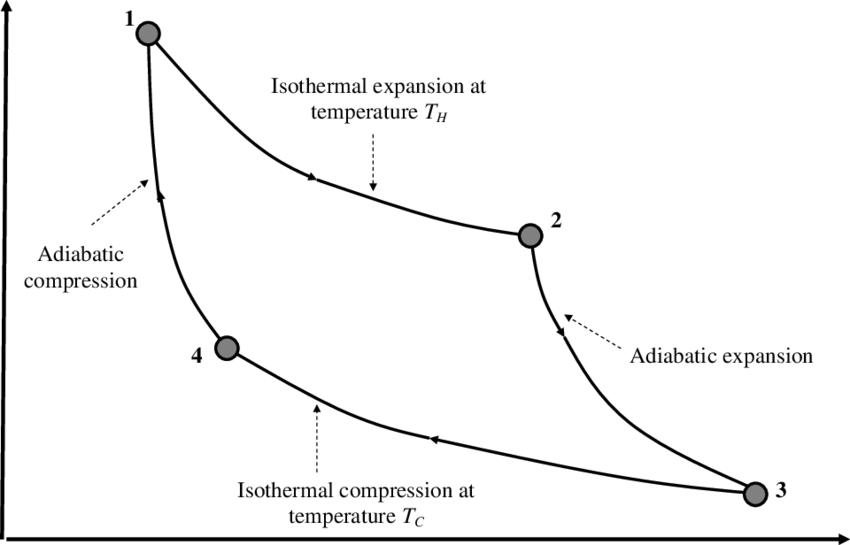
\includegraphics[width=8cm]{images/thermo/carnot.png}
\label {fig:carnot}
\end{figure}

By the first law, the work done by this heat engine on its surroundings is equal to the net heat gained by the system. Let $Q_H$ be the heat gained during step 1 and $Q_C$ be the heat released in step 4. Then the work done is $Q_H - Q_C$, and the efficiency is $$\eta = \frac{Q_H-Q_C}{Q_H} = 1-\frac{Q_C}{Q_H}.$$

We can calculate $Q_H$ as $$Q_H = W_{\text{by gas}} = \int \limits_{V_1}^{V_2} P dV = \int  \limits_{V_1}^{V_2} \frac{n R T_H}{V} dV = nR T_H \ln \left(\frac{V_2}{V_1}\right).$$ Similarly, we have $$Q_C = W_{\text{on gas}} = nRT_C \ln \left(\frac{V_3}{V_4}\right).$$

From the rule we derived early for adiabatic processes, we have 
\begin{align*}
T_H V_2^{K-1} &= T_C V_3^{K-1},\\ 
T_H V_1^{K-1} &= T_C V_4^{K-1},
\end{align*}
so 
$$\frac{V_2}{V_1} = \frac{V_3}{V_4}.$$

Thus, the heat ratio is
\begin{align*}
\frac{Q_C}{Q_H} &= \frac{T_C}{T_H}, 
\end{align*} 
so the efficiency is \begin{align}\eta &=1-\frac{T_C}{T_H}. \label{eff} \end{align}

We can now prove that the Kelvin-Planck statement must be false when the Clausius statement is false. Assume that we can transfer heat $Q_H$ from the reservoir at $T_C$ to $T_H$ with no other effects. We can then run the Carnot cycle and deliver heat $Q_C$ to the reservoir at $T_C$ and perform some work. The end result is that there was no net heat change at the reservoir at $T_H$, the reservoir at $T_C$ had some heat loss, and work was performed. This violates the Kelvin-Planck statement, as we have extracted heat from the reservoir at $T_C$ and converted it to work without any other effects. 

\subsection{Carnot's Theorem}
It turns out the Carnot cycle has the maximum possible efficiency of any heat engine. To prove this, consider the system in figure \ref{fig:proof}, where $\eta$ is the efficiency of the heat engine and $\eta'$ is the efficiency of the Carnot engine. The Carnot engine is run in reverse, as shown, and $T_1 > T_2$. If we have $\eta > \eta'$, the result is that heat is transferred from a cold reservoir to a hot one with no side effects. This directly violates the Clausius statement of the second law.

\begin{figure}[ht]
\centering
\caption{System for Carnot's Theorem Proof}
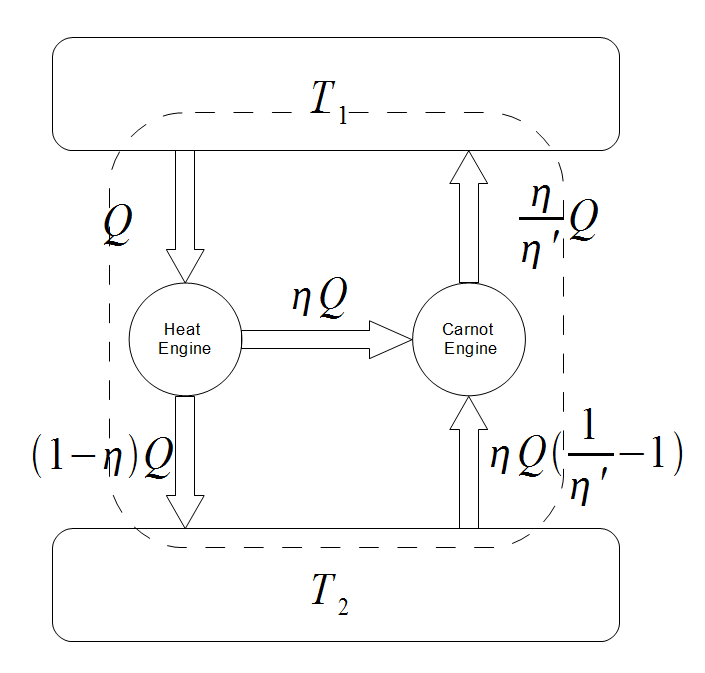
\includegraphics[width=6cm]{images/thermo/proof.png}
\label {fig:proof}
\end{figure}
\subsection{Entropy}
For our Carnot engine, we have $$\frac{Q_H}{T_H} = \frac{Q_C}{T_C}.$$ This means that the path integral of $\tfrac{\Delta Q}{T}$ is zero around our cycle. Based on this, we define the \textit{entropy} $S$ by the equation  $$\Delta S = \frac{\Delta Q}{T}.$$ Then $\Delta S = 0$ for the Carnot cycle (or any reversible transformation) and $\Delta S \geq 0$ in general.
\section {Entropy}
\subsection{The Second Law of Thermodynamics}
Recall that if the First Law of Thermodynamics is essentially a statement about what \textit{can} happen in a thermodynamical system, addressing energy and its conservation, then the Second Law is the one that dictates what will happen. We can think of the Second Law of Thermodynamics as giving a direction to time, philosophically, as it distinguishes processes that can happen while time progresses. The law itself can be phrased in a multitude of different ways, two of which are Clausius' and Kelvin's Postulates. Today, we'll phrase it differently: 
\begin{law}[The Second Law of Thermodynamics]
In a physical system, the \textit{entropy} $S$ of the system is non-decreasing, approaching a maximum value. 
\end{law}
We will be focused mostly on the nature of \textit{entropy}, our final state variable. Recall that a \textit{state variable} is one that only depends on the current configuration of particles in a system, and not on how the configuration was generated.

\subsection{Entropy and Statistical Mechanics}
To investigate entropy from a statistical mechanics perspective, we appeal to one of Boltzmann's results. First, define $\Omega$ to be the number of ways a state can be achieved/populated by the particles in the system. That is, given the energy distribution of the particles, $\Omega$ is the number of ways the atoms can be arranged to satisfy the conditions of the system. Boltzmann defines the entropy $S$ as 
\[
	S = k_B \ln \Omega,
\]
where $k_B$ is the \textit{Boltzmann constant}.
This allows one to derive the Third Law of Thermodynamics, where when we have one state ($\Omega = 1$) in a crystal lattice, the entropy of the system is zero. Not super relevant or particularly useful, but it's an interesting little corollary. 

We will now work in a \textit{micro-canonical ensemble}, where we fix the number of atoms $N$, the total energy of the system $E$, and the number of atoms in each of the $r$ energy states $n_k$, each associated with energy $\eps_k$. In variables, we have the following two constraints on our system: 
\[
	N = \sum_{k=1}^r n_k \quad E = \sum_{k=1}^r \eps_k n_k
\]
In general, in statistical mechanics (while working in equilibrium states), the micro-canonical ensemble is one of three main models used to describe a thermodynamical system. The others are the \textit{grand canonical ensemble} and the \textit{}
We can compute $\Omega$ and the entropy $S$ explicitly now: 
\[
	\Omega = \frac{N!}{n_1! n_2! \ldots n_r!} \implies S = k_B \ln \Omega = k_B \ln N! - k_B \sum_{k=1}^r \ln n_k!
\]
To maximize $S$, we have to use\ldots Lagrange multipliers! Consider the Lagrangian function
\[
	\lagr = S + \lambda\left(N - \sum_{k=1}^r n_k \right) + \mu \left(E - \sum_{k=1}^r \eps_k n_k\right) 
\]
and plugging in, we get 
\[
	\lagr = k_B \ln N! - k_B \sum_{k=1}^r \ln n_k! + \lambda\left(N - \sum_{k=1}^r n_k \right) + \mu \left(E - \sum_{k=1}^r \eps_k n_k\right) 
\]
We now compute $\pdv{\lagr}{n_j}$ and set it equal to 0: 
\[
	\pdv{\lagr}{n_j} = -k_B \pdv{}{n_j} \ln n_j! - \lambda - \mu \eps_j = 0
\]
So far, we've let the $n_i$s be integers, but in order to differentiate with respect to an $n_i$, we have to differentiate a factorial function. Since we're physicists, we're allowed to approximate, and so we can use \textit{Stirling's approximation}: 
\[
	n! \approx \left(\frac{n}{e}\right)^n \sqrt{2 \pi n} \implies \ln n! \approx n \ln n - n + \frac{1}{2} \ln 2\pi + \frac{1}{2} \ln n
\]
We're allowed to use this approximation that gets much better as $n_i$ gets very large (as we want them to be, usually), and so we can ``differentiate" $\ln n!$: 
\[
	\pdv{}{n} \ln n! \approx \ln n + 1 - 1 + \frac{1}{2n} \approx \ln n
\]
This gives us 
\[
	\pdv{\lagr}{n_j} = -k_B \ln n_j - \lambda - \mu \eps_j = 0
\]
If we pick different $n_j$, $n_k$, and we subtract them from each other, we have: 
\[
	\pdv{\lagr}{n_j} - \pdv{\lagr}{n_k} = -k_B \ln \frac{n_j}{n_k} - \mu (\eps_j - \eps_k) = 0 \implies k_B \ln n_j + \mu \eps_j = k_B \ln n_k + \mu \eps_k 
\]
Out of nowhere, we've found the invariant $k_B \ln n_k + \mu \eps_k$! With some foresight, let's let this constant be $k_B \ln A$: 
\[
	 k_B \ln n_k + \mu \eps_k = k_B \ln A \implies \ln \frac{n_k}{A} = -\frac{\mu \eps_k}{k_B} \implies n_k = A e^{-\frac{\mu \eps_k}{k_B}}
\]
This means the number of particles occupying state $k$ with energy $\eps_k$ is proportional to $e^{-\frac{\mu \eps_k}{k_B}}$ in equilibrium, derived from the fact that the entropy has to be maximized by the system. All we have to do now is to figure out what exactly $\mu$ is. 

The way we figure out what $\mu$ is by considering what happens what happens to the entropy $S$ when we move an atom from state $i$ to $j$. 
\begin{align*}
	dS &= k_B \ln \frac{N!}{n_1! n_2! \ldots (n_i-1)! \ldots (n_j+1)! \ldots n_r!} - k_B \ln \frac{N!}{n_1! n_2! \ldots n_i! \ldots n_j! \ldots n_r!} \\
	&= k_B \ln \frac{n_i}{n_j +1} \approx k_B \ln \frac{n_i}{n_j} = k_B \ln e^{\frac{\mu}{k_B}(\eps_j - \eps_i)} = \mu (\eps_j - \eps_i)
\end{align*}
This means that the change in entropy is directly proportional to the change in energy that the atom experiences, which is also the infinitesimal change in heat $\delta Q$! Assuming the process is reversible, we have $dS = \mu \delta Q$. We can make the final leap to claim that $\mu = \frac{1}{T}$, if we believe our definition of entropy from looking at Carnot cycles and heat engines.

This directly gives the most important thermodynamic fact in reversible processes, by way of the First Law of Thermodynamics: 
\begin{theorem}
The change in the internal energy $U$ is given by $dU = T dS - p dV$.
\label{thm-first}
\end{theorem}
This is a cool fact to tinker with and one can get all sorts of interesting relations amongst the state variables $p, V, T,$ and $S$. 

From this statistical perspective, entropy can be seen to be a measure of the ``disorder" of a system - the more ways a system can be populated, the higher the $\Omega$, and the higher the entropy. This can be interpreted (poorly) as the amount of ``chaos" present in the system, which is not a very useful way to think about the entropy. 

With this analysis of entropy, what we've also found is this underlying probability distribution of atoms occupying energy states, proportional to $e^{-\frac{\eps}{k_B T}}$, where $\eps$ is the energy of the state. This gives us an interesting probability distribution for ideal gases and how fast the atoms within them are moving. If we recall that the energy of a particle is $\frac{1}{2} mv^2$, where $v$ is the velocity, the probability distribution we have is now proportional to $e^{-\frac{mv^2}{2 k_B T}}$, normalized by some constant., which turns out to be
\[
    P(\vec v, d\vec v) = \left(\frac{m}{2\pi k_B T} \right)^{\frac{3}{2}} e^{-\frac{mv^2}{2 k_B T}}
\]
However, if we want to be working with a speed distribution, in our phase space, we have to ``integrate" this velocity distribution over all spheres of constant speed $v$, which gives us an extra term: 
\[
    P(v, dv) = \left(\frac{m}{2\pi k_B T} \right)^{\frac{3}{2}} 4\pi v^2 e^{-\frac{mv^2}{2 k_B T}}
\]
This gives us the \textit{Maxwell-Boltzmann speed distribution} for ideal gases, which is fairly accurate in real life and also gives us the energy for ideal gases as $U = \frac{3}{2} k_B T$, interestingly enough.

\section {Maxwell Relations}
\subsection{Introduction} In this lecture, we derive Maxwell's relations of thermodynamic potentials. These are useful because they relate difficult-to-measure quantities to others than can be easily measured. 
\subsection{Thermodynamic Potentials}
A \textit{thermodynamic potential} is a quantity used to represent some thermodynamic state in a system. Each thermodynamic potential represents a different ``type" of energy that the system has. There are \textit{natural variables} for each thermodynamic potential. When these variables are held constant, the associated potential is conserved.
\subsubsection{Internal Energy}
One example of a thermodynamic potential is \textit{internal energy}, which, as we know, is the energy of the system due to the motion of its constituent particles. Based on Theorem \ref{thm-first}, $U$ is conserved when $S$ and $V$ are both constant. Therefore, entropy and volume are the natural variables of internal energy. 
\subsubsection{Enthalpy}
The \textit{enthalpy} $H$ is another thermodynamic potential defined as $$ H = U + PV.$$ The enthalpy is the total heat content of the system - it measures the capacity to do non-mechanical or release heat.
 
We can derive $dH$ as follows. We have
\begin{align}
dH &= dU + P dV + V dP 
= TdS + VdP. \label{eq:H}
\end{align} 
Based on equation \ref{eq:H}, we can conclude that entropy and pressure are the natural variables of enthalpy.
\subsection{Helmholtz Free Energy}
Another thermodynamic potential is the \textit{Helmholtz free energy} $$F = U-TS.$$ This is the capacity to do useful work of any kind (mechanical and non-mechanical).

The differential form is 
\begin{align}
dF &= dU - TdS - SdT
= -PdV-SdT. \label{eq:F}
\end{align}
From equation \ref{eq:F}, we see that the natural variables of the Helmholtx free energy are volume and temperature.
\subsubsection{Gibbs Free Energy}
The final thermodynamic potential we will consider is the Gibbs free energy $$G = H-TS.$$ This measures how much non-mechanical work the system could do. We find that the differential form is 
\begin{align}
dG &= dH - TdS - S dT
= VdP - S dT \label{eq:G},
\end{align} 
so the natural variables of the Gibbs free energy are pressure and temperature.
\subsection{Derivation of Maxwell Relations}
\subsubsection{Internal Energy}
We write the internal energy $U$ as a function of its natural variables, $S$ and $V$, so the total differential is
$$dU = \left(\frac{\partial U}{\partial S} \right)_V dS + \left(\frac{\partial U}{\partial V} \right)_S dV.$$ Equating this to the differential form from Theorem \ref{thm-first} gives $$\left(\frac{\partial U}{\partial S} \right)_V dS + \left(\frac{\partial U}{\partial V} \right)_S dV = TdS - PdV,$$ so
\begin{align*}
\left(\frac{\partial U}{\partial V} \right)_S &= -P,\\
\left(\frac{\partial U}{\partial S} \right)_V &= T.
\end{align*}
Then we have
\begin{align*}
\left(\frac{\partial }{\partial S} \right)_V\left(\frac{\partial U}{\partial V} \right)_S &= -\left(\frac{\partial P }{\partial S} \right)_V,\\
\left(\frac{\partial }{\partial V} \right)_S\left(\frac{\partial U}{\partial S} \right)_V &= \left(\frac{\partial T}{\partial V} \right)_S.
\end{align*}
By Clairaut, we conclude that 
\begin{align}
 -\left(\frac{\partial P }{\partial S} \right)_V &= \left(\frac{\partial T}{\partial V} \right)_S \label{eq:m1}.
\end{align}
Equation \ref{eq:m1} is our first Maxwell relation.
\subsubsection{Enthalpy}
We use the same logic to derive the second Maxwell relation. Consider the enthalpy as a function of its natural variables, so that $H = H(S,P)$. Then we have 
$$dH = \left(\frac{\partial H}{\partial S} \right)_P dS + \left(\frac{\partial H}{\partial P} \right)_S dP = TdS+VdP,$$
so 
\begin{align*}
 \left(\frac{\partial H}{\partial S} \right)_P &= T, \\
  \left(\frac{\partial H}{\partial P} \right)_S &= V.
\end{align*}
Then 
\begin{align*}
\left(\frac{\partial }{\partial P} \right)_S\left(\frac{\partial H}{\partial S} \right)_P &= \left(\frac{\partial T }{\partial P} \right)_S,\\
\left(\frac{\partial }{\partial S} \right)_P\left(\frac{\partial H}{\partial P} \right)_S &= \left(\frac{\partial V }{\partial S} \right)_P,\\
\end{align*}
so 
\begin{align}
 \left(\frac{\partial T }{\partial P} \right)_S &= \left(\frac{\partial V }{\partial S} \right)_P \label{eq:m2}.
\end{align}
This is the second Maxwell relation.
\subsubsection{Helmholtz Free Energy}
We now consider the Helmholtz free energy as a function of its natural variables, so that $F = F(V,T)$. Then we have 
$$dF = \left(\frac{\partial F}{\partial V} \right)_T dV + \left(\frac{\partial F}{\partial T} \right)_V dT = -PdV-SdT,$$
so 
\begin{align*}
 \left(\frac{\partial F}{\partial V} \right)_T &= -P, \\
  \left(\frac{\partial F}{\partial T} \right)_V &= -S.
\end{align*}
Then 
$$ -\left(\frac{\partial P}{\partial T} \right)_V =
 \left(\frac{\partial }{\partial T} \right)_V\left(\frac{\partial F}{\partial V} \right)_T  = \left(\frac{\partial }{\partial V} \right)_T \left(\frac{\partial F}{\partial T} \right)_V = -\left(\frac{\partial S}{\partial V} \right)_T,
$$ so 
\begin{align}
 \left(\frac{\partial P }{\partial T} \right)_V &= \left(\frac{\partial S }{\partial V} \right)_T\label{eq:m3}.
\end{align}
This is the third Maxwell relation.
\subsubsection{Gibbs Free Energy}
Finally, we consider the Gibbs free energy as a function of its natural variables, so that $G = G(P,T)$. Then we have 
$$dG = \left(\frac{\partial G}{\partial P} \right)_T dP + \left(\frac{\partial G}{\partial T} \right)_P dT = V dP - S dT,$$
so 
\begin{align*}
 \left(\frac{\partial G}{\partial P} \right)_T &= V, \\
  \left(\frac{\partial G}{\partial T} \right)_P &= -S.
\end{align*}
Then 
$$ \left(\frac{\partial V}{\partial T} \right)_P =
 \left(\frac{\partial }{\partial T} \right)_P\left(\frac{\partial G}{\partial P} \right)_T  = \left(\frac{\partial }{\partial P} \right)_T \left(\frac{\partial G}{\partial T} \right)_P = -\left(\frac{\partial S}{\partial P} \right)_T,
$$ so 
\begin{align}
 \left(\frac{\partial V }{\partial T} \right)_P &= -\left(\frac{\partial S }{\partial P} \right)_T \label{eq:m4}.
\end{align}
This is the last Maxwell relation.
\subsection{Summary of Maxwell Relations}
We have derived the following Maxwell relations.
\begin{align*}
 -\left(\frac{\partial P }{\partial S} \right)_V &= \left(\frac{\partial T}{\partial V} \right)_S\\
\left(\frac{\partial T }{\partial P} \right)_S &= \left(\frac{\partial V }{\partial S} \right)_P\\
 \left(\frac{\partial P }{\partial T} \right)_V &= \left(\frac{\partial S }{\partial V} \right)_T\\
\left(\frac{\partial V }{\partial T} \right)_P &= -\left(\frac{\partial S }{\partial P} \right)_T
\end{align*}
These equations are useful because they relate difficult to measure quantities like $\left(\frac{\partial S }{\partial P} \right)_T$ to more easily measurable quantities like $\left(\frac{\partial V }{\partial T} \right)_P$. Note that they are not the only Maxwell relations; others can be derived for different thermodynamic potentials. 

\part{Waves and Modes}

\section{General Waves and the Wave Equation}

\subsection{The Wave Equation}
Consider the following nice happy wave - I've currently drawn it as a sinusoidal wave, but it really doesn't actually matter what shape it takes as long as it's continuous and satisfies a few of our assumptions (that we will list later):
\begin{center}
\begin{asy}
	import graph;
	size(200);
	real shift = 0.2;
	real down = -0.2;
	real f(real x) 
	{ 
		return sin(x); 
	} 
	Label f; 
	f.p=fontsize(6); 
	draw(graph(f,-2,3));
	for (int i = -2; i < 5; ++i)
	{
		draw( Circle( (i*0.5, f(i*0.5)), 0.1) );

		//label((string) (i+3), (i*0.5, f(i*0.5)), N*4);
	}
	label("$i$", (0.5, f(0.5)), dir(135)*4);
	label("$i-1$", (0, 0), dir(150)*4);
	label("$i+1$", (1, f(1)), N*4);
	draw((0.5+shift, f(0.5))--(0.5+shift,0), Arrows);
	label("$\Delta y$", (0.5+shift, f(0.5))--(0.5+shift,0), E); 
	draw((0, down)--(0.5, down), Arrows);
	label("$\Delta x$", (0, down)--(0.5, down), S);
\end{asy}
\end{center}
What I've done here is that I've essentially divided up the wave into discrete particles, as is the case in physics whenever we derive something continuous (we start with distinct pieces, and try to argue what happens when we make those pieces really really small). This wave is physically speaking, moving in an elastic string - and we assume that it has a constant tension $T$ and mass density per unit length $\mu$. We're also going to assume that all these little pieces of the wave only move up and down, and not horizontally - effectively, this is a wave in one dimension. We also take $\pdv{y}{x} << 1$ - this means we're dealing with what's called a linear wave, and it's a decent approximation for reality. Finally, we will neglect the effects of gravity on the string during this derivation. \\
Let's get started. First, we're going to pick any of these discrete masses at random, say $i$. (I've numbered them arbitrarily in the diagram.) We're going to use Newton's Second Law on $i$, and so here's our free body diagram on point mass $i$:
\begin{center}
\begin{asy}
size(100);
dot((0,0)); 
draw((0,0)--dir(30), Arrow); 
draw((0,0)--dir(225), Arrow); 
label("$\vec{F_1}$", (0,0)--dir(30));
label("$\vec{F_2}$", (0,0)--dir(225));
\end{asy}
\end{center}
These forces come from the tension in the string exerted in the directions of point masses $i-1$ and $i+1$. Notice that while both forces $\vec F_1,\vec F_2$ have the same magnitude by our assumption (they both have the magnitude of the tension, $T$), they point in different directions. Let's define $y_i$ to be the height of the $i$th particle. Assuming that the horizontal motion is negligible, we have by Newton's Second Law:
$$F_{y1} = T \sin \theta_1 = T \cdot \frac{y_{i+1}-y_i}{\sqrt{\Delta x^2 + (y_{i+1} - y_i)^2}} $$
$$F_{y2} = -T \sin \theta_2 = -T \cdot \frac{y_{i}-y_{i-1}}{\sqrt{\Delta x^2 + (y_{i} - y_{i-1})^2}} $$
$$\rightarrow F_{net} = \mu \Delta x \frac{\partial^2 y_i}{\partial t^2} =  T \left(\frac{y_{i+1}-y_i}{\sqrt{\Delta x^2 + (y_{i+1} - y_i)^2}} -  \frac{y_{i}-y_{i-1}}{\sqrt{\Delta x^2 + (y_{i} - y_{i-1})^2}} \right)$$
All we did here was project these forces into the vertical direction, and from the diagram, we more or less approximated the angle of the force to be essentially in the direction from one point to its neighboring point, hence all the Pythagorean Theorem-esque square roots.\\
With our linear wave approximation, we have that $\Delta y << \Delta x$, and therefore we can ignore all second-order terms involving differences in $y$. That allows us to simplify down quite a bit:
$$ T \left(\frac{y_{i+1}-y_i}{\Delta x} -  \frac{y_{i}-y_{i-1}}{\Delta x} \right) = \mu \Delta x \frac{\partial^2 y_i}{\partial t^2} $$ Here comes the part where we shift from discrete particles to continuous pieces. If we let $\Delta x$ go to zero, these individual fractions basically become first derivatives of $y$ with respect to $x$. However, since we're subtracting them, and they're almost the same (differing only by a small amount), their difference is effectively the derivative of the first derivative with respect to $x$, times $\Delta x$. In other words, we have:
$$T \pddv{y_i}{x} \Delta x = \mu \Delta x \pddv{y_i}{t} $$Simplifying:
$$T \pddv{y_i}{x} = \mu \pddv{y_i}{t} $$This is all true for a mechanical wave, but often times we want to relate this to the speed $v$ of the wave through the medium, in which case you'll see this as
$$ \pddv{y}{x} = \frac{1}{v^2} \pddv{y}{t}$$
Notice that $T = \mu v^2$. This relation will be very useful going forward.\\
What solutions satisfy the equation? It turns out that a wide family of functions do - specifically, any function moving to the right at speed $v$ will satisfy the wave equation, and by symmetry, so will any function moving to the left. To be explicit, any function of the form $y(x, t) = f(x \pm vt)$ will satisfy the wave equation. We can check this explicitly: letting $y(x,t) = f(x \pm vt)$, we have:
$$ \pddv{y}{x} = f''(x\pm vt) \quad \pddv{y}{t} = v^2 f''(x\pm vt)$$
$$ \rightarrow \pddv{y}{x} = f''(x\pm vt) = \frac{1}{v^2} \pddv{y}{t} = \frac{1}{v^2} \cdot v^2 f''(x\pm -vt)$$

\subsection{Energy in a Wave}
Let's now derive an expression for the energy stored in the wave. Energy stored in a mechanical wave comes in two forms - kinetic energy and potential energy, so we will calculate these parts separately. 
\begin{center}
\begin{asy}
	import graph;
	size(200);
	real shift = 0.2;
	real down = -0.2;
	real f(real x) 
	{ 
		return sin(x); 
	} 
	Label f; 
	f.p=fontsize(6); 
	draw(graph(f,-2,3));
	for (int i = -2; i < 5; ++i)
	{
		draw( Circle( (i*0.5, f(i*0.5)), 0.1) );

		//label((string) (i+3), (i*0.5, f(i*0.5)), N*4);
	}
	dot((0.75, f(0.75))); 
	draw((0.75, f(0.75))--dir(35)+(0.75, f(0.75)), Arrow); 
	draw((0.75, f(0.75))--dir(214)+(0.75, f(0.75)), Arrow); 
	label("$i$", (0.5, f(0.5)), dir(135)*4);
	label("$i+1$", (1, f(1)), N*4);
\end{asy}
\end{center}
Revisiting our diagram above, we can consider the energy of a particle $i$ in the string. The kinetic energy is fairly straightforward - we note that the particle has mass $\mu \Delta x$ and velocity $\pdv{y_i}{t}$, so in general the kinetic energy of the particle $K = \frac{1}{2} \mu \Delta x \left( \pdv{y}{t} \right)^2$. \\
What of the potential energy? We can consider the work that the forces do on the "link" between particles $i$ and $i+1$ in a time $\Delta t$, and in fact we know that the potential energy in this wave is stored in the interactions between parts of the string. From the previous section, we know that these forces have the same magnitude in the $y$-direction, $T \cdot \frac{y_{i+1} - y_i}{\Delta x}$. However, the distance (vertically) traveled in a time $\Delta t$ is different for each particle, so this difference gives us a net work:
$$ W_{net} = -T \cdot  \frac{y_{i+1} - y_i}{\Delta x} \cdot \pdv{y_{i+1}}{t} \Delta t + T \cdot \frac{y_{i+1} - y_i}{\Delta x} \cdot \pdv{y_i}{t} \Delta t$$
As we let $\Delta x$ go to zero, we can consider that $\frac{y_{i+1} - y_i}{\Delta x} = \pdv{y}{x}$. Simplifying, we have that in general 
\begin{align*}
W_{net} &= -T \Delta t \cdot \pdv{y}{x} \cdot \left(\pdv{y_{i+1}}{t} - \pdv{y_i}{t} \right) \\
&= -T \Delta t \cdot \pdv{y}{x} \cdot \pdv{}{t}\left(\pdv{y}{x} \Delta x\right) \\
&= -\Delta \left( \frac{1}{2} T \left( \pdv{y}{x} \right)^2 \right)  \Delta x
\end{align*}
where the $\Delta$ signifies a small change in the quantity, otherwise known as a differential\footnote{This is a bit of an abuse of notation, but Osborne used this notation during the lecture for the ease of motivating the next step.}. 
We can now apply the Work-Energy Theorem to note that 
$$ \Delta U = - W_{net} = \Delta \left( \frac{1}{2} T \left( \pdv{y}{x} \right)^2 \right)  \Delta x \rightarrow U =  \frac{1}{2} T \left( \pdv{y}{x} \right)^2 \Delta x$$
With this explicit computation of the kinetic and potential energies, we can now state that the total energy of the particle is 
$$ E = K + U = \left[\frac{1}{2} \mu \left( \pdv{y}{t} \right)^2 + \frac{1}{2} T \left( \pdv{y}{x} \right)^2 \right] \Delta x $$
It's actually more convenient to find the energy per unit length $\epsilon$, since we don't have that pesky $\Delta x$ term:
$$ \epsilon = \frac{1}{2} \mu \left( \pdv{y}{t} \right)^2 + \frac{1}{2} T \left( \pdv{y}{x} \right)^2 $$
The total energy over a length of the wave, then, the energy is clearly the integral of this with respect to $x$:
$$ E = \int_{x_1}^{x_2} \frac{1}{2} \mu \left( \pdv{y}{t} \right)^2 + \frac{1}{2} T \left( \pdv{y}{x} \right)^2 \, dx$$
Power per unit length $p$ (energy delivered per unit length per unit time) can be attained by taking the derivative of the energy density: 
\begin{align*}
p &= \pdv{}{t} \left[\frac{1}{2} \mu \left( \pdv{y}{t} \right)^2 + \frac{1}{2} T \left( \pdv{y}{x} \right)^2  \right] \\
&= \mu \pdv{y}{t} \pddv{y}{t} + T \pdv{y}{x} \frac{\partial^2 y}{\partial x \, \partial t}  \\
&= T \left[\pdv{y}{t} \pddv{y}{x} + \pdv{y}{x} \frac{\partial^2 y}{\partial x \, \partial t} \right] \\
&= T \pdv{}{x} \left[\pdv{y}{x} \pdv{y}{t} \right] 
\end{align*}
where we use the wave equation to replace $\pddv{y}{t}$ with $v^2 \pddv{y}{x}$ and observe we that can use the reverse of the product rule to simplify. From this, power in the wave can be obtained from this expression by integrating the power density with respect to $x$, or by differentiating energy with respect to $t$.\\
From this point forward, we will assume the function is also all moving in one direction, so $y(x, t) = f(x \pm vt)$ (ie. the wave is either only moving to the right or to the left at speed $v$). Power can be attained by considering that if the wave moves in one direction through a boundary, the energy delivered to that boundary is the energy density times $v \Delta t$, where $\Delta t$ is the time interval. Therefore, we can simply multiply energy density by the speed of the wave to attain the power: 
$$P = \left[\frac{1}{2} \mu \left( \pdv{y}{t} \right)^2 + \frac{1}{2} T \left( \pdv{y}{x} \right)^2 \right] v $$
If the entirety of the wave is moving in one direction, we can exploit the fact that $\left( \pdv{y}{x} \right) = \frac{1}{v^2} \left( \pdv{y}{t} \right)$, to attain that the energy density is: 
\[
	\epsilon = T [f'(x \pm vt)]^2
\]
and the expression for energy in a length of the wave can be simplified slightly to the integral of this expression. 

\subsection{Energy in Two Waves and Interference} 
Consider now a function representing a composition of two waves moving in opposite directions, of the form $y(x, t) = f(x-vt) + g(x+vt)$. Notice that when we can calculate the energy per unit length and the power per unit length, as follows: 
\begin{align*}
	\epsilon &= \frac{1}{2} \mu v^2 (-f' + g')^2 + \frac{1}{2} T (f' + g')^2 \\
	&= T (f'^2 + g'^2)\\
	p &= T \pdv{}{x} \left[(f' + g') (-v f' + v g') \right] \\
	&= Tv \pdv{}{x} (g'^2 - f'^2)
\end{align*}
These expressions have no cross-term; that is, the energies of these functions are not dependent on a term consisting of both functions related to $f$ and $g$ and therefore one can separate the energies into two distinct components - one of the energy from $f(x-vt)$ and the other from $g(x+vt)$. While these waves will interfere with each other, it's important to note that these waves are independent and propagate through each other and don't actually combine with each other. 


\section{Sinusoidal Waves and Boundaries}

\subsection{Sinusoidal Waves}
We now turn our attention to a particular class of waves. Sinusoidal waves are shaped like sine/cosine functions and generally take the form $y(x, t) = A \sin (kx - \omega t)$, where we define $A$ to be the amplitude, $k$ to be the wave number, and $\omega$ to be the angular frequency. 
\begin{center}
\begin{asy}
	import graph;
	size(200);
	real shift = 0.2;
	real down = -0.2;
	real f(real x) 
	{ 
		return 3*sin(pi*x/4); 
	} 
	Label f; 
	f.p=fontsize(6); 
	draw(graph(f,0,12));
	draw((0,0)--(12, 0), linetype("8 8")); 
	draw((10, 3)--(10,0), Arrows); 
    label("$A$", (10, 3)--(10,0), E); 
    draw((2, 3.5)--(10,3.5), Arrows);
    label("$\lambda$", (10, 3.5)--(2,3.5), N); 
    
    dot((0,0), blue); dot((4,0), blue); dot((8,0), blue); dot((12,0), blue);
    dot((2,3), red); dot((6,-3), red); dot((10, 3), red); 
\end{asy}
\end{center}
We also define the wavelength $\lambda$, the period $\tau$,\footnote{usually denoted with $T$, but not to be confused with the tension $T$} and the frequency $f$.\footnote{usually denoted with $\nu$, but not to be confused with the velocity $v$} Sinusoidal waves are periodic, so the period $\tau$ is the time between the instances where the wave at a certain point is the same. The wavelength $\lambda$ is the distance between equal parts of the periodic wave (ie. between two crests or two troughs), and the frequency $f$ is the number of periods of the wave that pass by a certain point per unit time. Sinusoidal waves, by themselves are also moving with a speed $v$. \\
We can define a number of relations among these variables: 
\[
	\lambda = \frac{2\pi}{k} \quad f = \frac{\omega}{2\pi} = \frac{1}{T} \quad v = \frac{\omega}{k} = \frac{\lambda}{T} = \sqrt{\frac{T}{\mu}}
\]
Let's apply our formulas for energy from the last lecture to find the energy stored in one wavelength in a typical sinusoidal wave. Recall that the energy density $\epsilon$ is: 
\begin{align*}
\epsilon &= \frac{1}{2} \mu \left( \pdv{y}{t} \right)^2 + \frac{1}{2} T \left( \pdv{y}{x} \right)^2 \\
&= \frac{1}{2} \mu \omega^2 A^2 \cos^2 (kx - \omega t) + \frac{1}{2} T k^2 A^2 \cos^2 (kx - \omega t) \\
&= Tk^2 A^2 \cos^2 (kx-\omega t) 
\end{align*}
where this last simplification comes from noting that $Tk^2 = \mu \omega^2$ and combining terms. Integrating, we now have: 
\[
	E = \int_0^\lambda Tk^2 A^2 \cos^2 (kx-\omega t) \, dx = \frac{1}{2} TA^2k^2 \lambda = \pi TA^2 k = 2\pi^2 A^2 \mu f v 
\]
We can also find the power in this sinusoidal wave: 
\[
	P = Tk^2 A^2v \cos^2 (kx-\omega t) = T k \omega A^2 \cos^2 (kx - \omega t) = \mu \omega^2 A^2 \cos^2 (kx - \omega t) = 4\pi^2 \mu f^2 A^2 \cos^2 (kx - \omega t) 
\]
We can see from this that the maximum power in the wave is concentrated at the points where $kx - \omega t = n \pi$ for some integer $n$, which are the points that lie on the center line of the wave. These points are called the nodes of the wave (marked in blue). The points of maximum displacement in the wave are called the antinodes, and form this expression we see that the antinodes have zero energy and power instantaneously flowing out of these points (marked in red). In general, for any wave, it's worth noting that the energy (and hence, power, energy density, etc.) is always proportional to the amplitude squared. \\
It's also worth looking at the average power from this propagating wave. If we note that the average value of $\sin^2 (kx-\omega t)$ on one wavelength is $\frac{1}{2}$, we can find the average power over the wave as: 
\[
	\expval{P} = 2\pi^2 \mu f^2 A^2
\]
We can also look specifically at the contributions of kinetic and potential energy density to the energy density and power: 
\begin{align*}
\epsilon_K &= \frac{1}{2} \mu \omega^2 A^2 \cos^2 (kx - \omega t)\\
K &= \frac{1}{4} TA^2k^2 \lambda = \frac{1}{2} \pi TA^2 k = \pi^2 A^2 \mu f v  \\
P_K &= \frac{1}{2} T k \omega A^2 \cos^2 (kx - \omega t) = 2\pi^2 \mu f^2 A^2 \cos^2 (kx - \omega t) \\
\expval{P_K} &= \pi^2 \mu f^2 A^2 
\end{align*}
\begin{align*}
\epsilon_U &= \frac{1}{2} T k^2 A^2 \cos^2 (kx - \omega t)\\
U &= \frac{1}{4} TA^2k^2 \lambda = \frac{1}{2} \pi TA^2 k = \pi^2 A^2 \mu f v  \\
P_U &= \frac{1}{2} T k \omega A^2 \cos^2 (kx - \omega t) = 2\pi^2 \mu f^2 A^2 \cos^2 (kx - \omega t) \\
\expval{P_U} &= \pi^2 \mu f^2 A^2 
\end{align*}
From this, we see that the kinetic and potential energy flows are exactly the same and each contribute half of the energy. They are also in phase, meaning that they occur at the same place in each period. We will see that this is not the case for all waves. 
\subsection{Standing Waves}
In the last section, we specifically talked about propagating sinusoidal waves, which move all in one direction. We will now move to talk about standing waves, which take the form $y(x, t) = A \sin (kx) \cos (\omega t)$, and appear to oscillate in place. Standing waves appear to have their nodes and antinodes at the same positions at all times $t$. 
\begin{center}
\begin{asy}
	import graph;
	size(200);
	real shift = 0.2;
	real down = -0.2;
	real f(real x) 
	{ 
		return 3*sin(pi*x/4); 
	} 
	real g(real x)
	{
		return -3*sin(pi*x/4);
	}
	Label f; 
	f.p=fontsize(6); 
	draw(graph(f,0,12));
	Label g; 
	g.p=fontsize(6);
	draw(graph(g,0,12), linetype("4 4"));
	draw((0,0)--(12, 0), linetype("8 8")); 
	draw((10, 3)--(10,0), Arrows); 
    label("$A$", (10, 3)--(10,0), E); 
    draw((2, 3.5)--(10,3.5), Arrows);
    label("$\lambda$", (10, 3.5)--(2,3.5), N); 
    
    dot((0,0), blue); dot((4,0), blue); dot((8,0), blue); dot((12,0), blue);
    dot((2,3), red); dot((2,-3), red);
    dot((6,3), red); dot((6,-3), red); 
    dot((10, 3), red); dot((10,-3), red);
\end{asy}
\end{center}
Using the sum-to-product identities for trigonometric functions, we can decompose any standing wave as follows: 
\[
 \sin(A+B) + \sin(A-B) = 2 \sin A \cos B  
\]
\[
	\Rightarrow \sin kx \cos \omega t = \frac{1}{2} ( \sin (kx - \omega t) + \sin (kx + \omega t) ) 
\]
Standing waves are a composition of two propagating waves moving in opposite directions, but with the same wave number and angular frequency. This means that we can't use the same formulas for the power that we used in the previous section, as standing waves have components that are moving in opposite directions. However, we can compute the energy density normally: 
\begin{align*}
\epsilon &= \frac{1}{2} \mu \left( \pdv{y}{t} \right)^2 + \frac{1}{2} T \left( \pdv{y}{x} \right)^2 \\
&= \frac{1}{2} \mu \omega^2 A^2 \sin^2(kx) \sin^2(\omega t) + \frac{1}{2} T k^2 A^2 \cos^2 (kx) \cos^2 (\omega t) 
\end{align*}
Integrating over one wavelength, we can find the total energy stored in the wave:
\begin{align*}
E &= \int_0^\lambda \frac{1}{2} \mu \omega^2 A^2 \sin^2(kx) \sin^2(\omega t) + \frac{1}{2} T k^2 A^2 \cos^2 (kx) \cos^2 (\omega t) \, dx \\
&= \int_0^\lambda \frac{1}{2} T k^2 A^2 \sin^2(kx) \sin^2(\omega t) \, dx + \int_0^\lambda \frac{1}{2} T k^2 A^2 \cos^2 (kx) \cos^2 (\omega t) \, dx \\
&= \frac{1}{2} T k^2 A^2 \cdot \frac{\lambda}{2} \cdot (\sin^2 (\omega t) + \cos^2 (\omega t)) \\
&= \frac{1}{4} Tk^2 A^2 \lambda = \pi^2 A^2 \mu f v
\end{align*}
Notice that the energy in a standing wave is half of that in a propagating wave, and one fourth of the expected energy from two propagating waves. This is due to the interference of the two propagating waves canceling each others' energy contributions. \\
We can also look at the power density and the kinetic and potential energy contributions to the power density. Recall that the power density $p$ is: 
\[
	p = T \pdv{}{x} \left[\pdv{y}{x} \cdot \pdv{y}{t} \right] = \pdv{\epsilon}{t} 
\]
First, the overall power density contribution: 
\begin{align*}
	p &= T \pdv{}{x} \left[k A \cos (kx) \cos (\omega t) \cdot - \omega A \sin (kx) \sin (\omega t) \right] \\
	&= -\frac{1}{4} Tk\omega A^2 \pdv{}{x} (\sin (2kx) \sin (2\omega t)) \\
	&= -\frac{1}{2} Tk^2 \omega A^2 \cos (2kx) \sin (2\omega t)
\end{align*}
Looking at the the contributions from the kinetic and potential parts: 
\begin{align*}
	p_K = \pdv{}{t} \left[ \frac{1}{2} \mu \left(\pdv{y}{t} \right)^2 \right] &= \mu \pdv{y}{t} \pddv{y}{t} \\
	&= \mu \cdot -\omega A \sin (kx) \cos (\omega t) \cdot -\omega^2 A \sin(kx) \sin (\omega t) \\
	&= \frac{1}{2} \mu \omega^3 A^2  \sin^2 (kx) \sin (2 \omega t) \\
	&= \frac{1}{2} Tk^2 \omega A^2 \sin^2 (kx) \sin (2\omega t) 
\end{align*}
\begin{align*}
	p_U = \pdv{}{t} \left[ \frac{1}{2} T \left(\pdv{y}{x} \right)^2 \right] &= T \pdv{y}{x} \mpddv{y}{x}{t} \\
	&= T \cdot -k A \cos (kx) \sin (\omega t) \cdot k\omega A \cos(kx) \cos (\omega t) \\
	&= -\frac{1}{2} Tk^2 A^2 \omega  \cos^2 (kx) \sin (2 \omega t)
\end{align*}
By conservation of energy, the two expressions for potential and kinetic power density are expected to (and in fact, do) combine to make total power density, but they are obviously not the same expression. The locations of maximum kinetic power density occur when $kx = \frac{\pi}{2} + \pi n $ (the antinodes), whereas the locations of maximum potential energy occur when $kx = \pi n$ (the nodes). This indicates that the distributions of kinetic and potential energy are out of phase by $\frac{\pi}{2}$, unlike that of the propagating wave. 
\subsection{Boundaries and Medium Changes}
When a mechanical wave hits a rigid boundary, the wave is reflected back (which can be seen from demonstrations). What happens when a propagating wave moves between mediums of different densities? 
\begin{center}
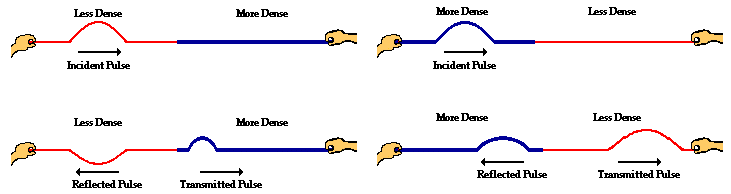
\includegraphics[scale=0.8]{images/waves/mediumchange.png}\\
\end{center}
As seen, when a propagating wave is incident on this boundary, a wave is transmitted through to the other medium, but a wave is also reflected back into the first medium. If we let the mediums have different mass densities $\mu_1$ and $\mu_2$ but with constant tension in the medium, the velocities will obviously be different. However, the frequency of all the waves will be constant - note that if $f$ periods of the wave move through the boundary, exactly $f$ periods will have to leave it - hence, the angular frequencies and frequencies of all the waves will be the same, but everything associated with length will be different between the two mediums. With this in mind, we can describe the net waves in each of the two mediums as the following: 
\[
	y_1(x, t) = A_I \sin (k_1 x - \omega t) + A_R \sin (k_1 x - \omega t) 
\]
\[
	y_2(x, t) = A_T \sin (k_2 x - \omega t) 
\]
where $k_i$ are the wave numbers of the wave in the first/second mediums, and $A_I$, $A_R$, and $A_T$ are the amplitudes of each of the incident, reflected, and transmitted waves, respectively. If we assume that the waves are continuous and differentiable at the boundary ($x=0$), we can obtain the following expressions for the amplitudes of the reflected and transmitted wave in terms of the amplitude of the incident wave: 
\[
	A_R = \frac{k_1 - k_2}{k_1 + k_2} A_I = \frac{v_2 - v_1}{v_1+ v_2} A_I \quad A_T = \frac{2k_1}{k_1 + k_2} A_I = \frac{2v_2}{v_1+v_2} A_I
\]
From this we see that if the speed of the wave in the second medium is lesser than that in the first (meaning that the medium is more dense), the reflected wave will have a negative amplitude, ie. the reflected wave will be inverted. In general, while we only derived this for sinusoidal waves, if a general incident wave is moving from a less dense to a more dense medium, the reflected wave will be inverted. \\


\section{A Digression on Sound}
\subsection{Sound Waves}
Generally, in this class most waves are transverse - ie. the motion is perpendicular to the medium in which the motion is taking place. Sound waves are a notable exception - these are longitudinal waves with motion parallel to the medium. This means the places of highest intensity are compressions in the medium and places of lowest intensity are rarefactions.
\begin{center}
	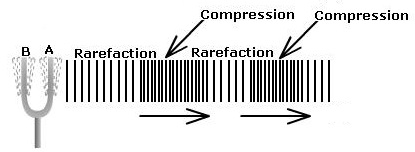
\includegraphics[scale=1.5]{images/waves/soundwaves.jpg}\\
\end{center}
Sound waves exist in three-dimensional space, and so the wavefront of a sound wave is the surface of a sphere, of which the total energy in the sound wave must be distributed over. The surface area of the wavefront is proportional to the square of the distance $r$ from the source, so the intensity of the wave goes down as $\frac{1}{r^2}$. In order to achieve this, we model the wave as a spherical Bessel wave of the form $y(r, t) = \frac{\sin(kr-\omega t)}{r}$, where $r$ is the distance from the source. This is derived from the fact that intensity is proportional to energy times amplitude $A$ squared, and hence $A \propto \frac{1}{r}$. The "amplitude" can also be thought of how far points in the medium are displaced from equilibrium.
\section{Interference and a "Double Slit Experiment"}
It's instructive to see how sound waves interfere with each other, especially since these are spherical waves. This is exemplified in the sound version of the "double-slit experiment", where we place two speakers a distance $d$ apart and measure intensity of the sound on a line a distance $D$ away. 
\begin{center}
	\begin{asy}
		import graph;
		size(175); 
real wall = 5; 
real D = 9;
real y = 4;
real d = 1.5;
pair sp1 = (0, d); 
pair sp2 = (0, -d); 
draw(Circle(sp1, 0.1)); 
draw(Circle(sp2, 0.1)); 
draw((D, -wall)--(D, wall)); 
draw((0, wall)--sp1+dir(90)*0.2, linetype("4 4")); 
draw((0, -wall)--sp2+dir(270)*0.2, linetype("4 4")); 
draw(sp2+dir(90)*0.2--sp1+dir(270)*0.2, linetype("4 4")); 
dot((D, y)); 
dot((0, 0)); 
draw((0,0)--(D, 0), linetype("4 4")); 
draw((0, -4)--(D, -4), Arrows);
dot((D, 0));
draw((D+0.5, 0)--(D+0.5, y), Arrows); 
draw((-0.5, d)--(-0.5, -d), Arrows);
draw(sp1+dir(25)*0.2--(D, y));
draw(sp2+dir(40)*0.2--(D, y));
draw((0, 0)--(D,y), linetype("8 8")); 
for (int r = 0; r < 3; ++r)
{
	draw(arc(sp1, 0.4+0.2*r, 60, -60));
	draw(arc(sp2, 0.4+0.2*r, 60, -60));
}
label("$d$", (-0.5, d)--(-0.5, -d), W);
label("$R$", (0,0)--(D,y), dir(140));
label("$y$", (D+0.5, 0)--(D+0.5, y), E);
label("$D$", (0+0.2, -4)--(D-0.2, -4), S);
label("$\theta$", (0,0), dir(12)*7);
	\end{asy}
\end{center}
For some arbitrary point $y$ from the center on the line, let $R$ be the distance from the midpoint of the sound sources to this point, and $\theta$ to be the angle between the line to this point and the perpendicular to the line. \\
Using our model for sound waves (Bessel waves) discussed in the previous section, from our arbitrary point, we can compute the wave experienced at this point as the sum of two sound waves (in exponential form): 
\[
	u(y, t) = \frac{1}{2} \left[ \frac{e^{i \left(k \sqrt{D^2 + \left(y - \frac{d}{2} \right)^2} - \omega t\right)}}{\sqrt{D^2 + \left(y - \frac{d}{2} \right)^2}} + \frac{e^{i \left(k \sqrt{D^2 + \left(y + \frac{d}{2} \right)^2} - \omega t\right)}}{\sqrt{D^2 + \left(y + \frac{d}{2} \right)^2}} \right] 
\]
Note that taking the imaginary part of this expression will result in the sum of the waves we desire. Since we're mostly concerned where the maximum/minimum intensities are, we can use this exponential form of the wave to describe the wave. We also include the factor of $\frac{1}{2}$ to normalize the wave - it will scale the actual magnitude of the wave down by a factor of $2$, but it will not have an effect on which points will have a maximum/minimum intensity.\\
We will now make the approximation that $D >> d$, and use the Taylor series of the square root term, using the two lowest-order terms: 
\begin{align*}
	\sqrt{D^2 + \left(y - \frac{d}{2} \right)^2} &= \sqrt{D^2 + y^2 - yd + \left( \frac{d^2}{4} \right)} \\
	&= R \sqrt{1 - \frac{yd}{R^2} + \frac{d^2}{4R^2}} \\
	&= R \left[1 + \frac{1}{2}\left(\frac{d^2}{4R^2} - \frac{yd}{R^2}\right) - \frac{1}{8}\left(\frac{d^2}{4R^2} - \frac{yd}{R^2}\right)^2 + \ldots \right] \\
	&\approx R\left[1 - \frac{yd}{2R^2} \right] 
\end{align*}
We plug this approximation back into our original expression, using a similar approximation for the other square root. We also use $R$ to approximate the radicals in the denominator: 
\begin{align*}
	u(y, t) &= \frac{1}{2R} \left[ e^{i \left(kR - \frac{kyd}{2R} - \omega t\right)} + e^{i \left(k R + \frac{kyd}{2R} - \omega t\right)} \right] \\
	&= \frac{e^{i \left(kR - \omega t\right)}}{2R} \left[ e^{- i\frac{kyd}{2R}} + e^{i\frac{kyd}{2R}} \right] \\
	&= \frac{e^{i \left(kR - \omega t\right)}}{R} \cos \left( \frac{kdy}{2R}\right) = \frac{e^{i \left(kR - \omega t\right)}}{R} \cos \left( \frac{kd}{2} \sin \theta \right)
\end{align*}
From this, we can see that we can maximize/minimize the amplitude, and thus, the intensity of the sound if we maximize/minimize the cosine term. \\
When the intensity of the sound is observed to be at a maximum, we should have that the argument of the cosine function should be $n \pi$ for some integer $n$ to have a maximum magnitude. This implies:
\[
	\frac{kd}{2}\sin \theta = n \pi  \rightarrow \frac{\pi d}{\lambda}\sin \theta = n \pi \rightarrow d\sin \theta = \lambda n 
\] 
Similarly, when the intensity of the sound is observed to be a minimum, the argument of the cosine function should be $\left( n + \frac{1}{2} \right) n$ for some integer $n$, so the magnitude of the intensity is minimized when:
\[
	\frac{kd}{2}\sin \theta = \left( n + \frac{1}{2} \right) \pi  \rightarrow \frac{\pi d}{\lambda}\sin \theta = \left( n + \frac{1}{2} \right) \pi \rightarrow d\sin \theta = \lambda \left( n + \frac{1}{2} \right) 
\]
\subsection{Modulation and Carrier Waves}
When dealing with sound waves in particular, we can see what happens when we look at interference of sound waves with different frequencies instead of looking at spatial differences in the double-slit experiment.\\
Consider two waves with angular frequencies of 12 Hz and 2 Hz. (These are not sound waves you can hear, but it doesn't impede our mathematical calculations.) If we consider the sum of two waves (ignoring spherical nature of sound waves), we see that, by sum-to-product identities:
\[
	\sin(12t) + \sin(2t) = 2\sin(7t)\cos(5t)
\]
If we look at the graph of this function: 
\begin{center}
	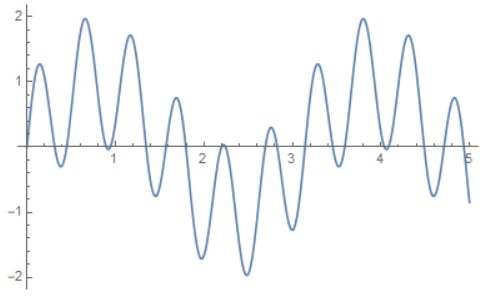
\includegraphics[scale=1]{images/waves/modulation1.jpg}\\
\end{center}
we see that the overall wave has an angular frequency of 2 Hz, but inside the wave itself there are waves oscillating at a frequency of 12 Hz still. If one were to play a scaled up version of these waves to audible frequencies, one could hear both of these distinct sounds (try, for example, a high C and a low A). \\
Let's also consider two waves with closer angular frequencies, say 22 Hz and 20 Hz. By a similar manipulation we can see that: 
\[
	\sin(22t) + \sin(20t) = 2\sin(21t)\cos(t)
\]
See the graph of this function below: 
\begin{center}
	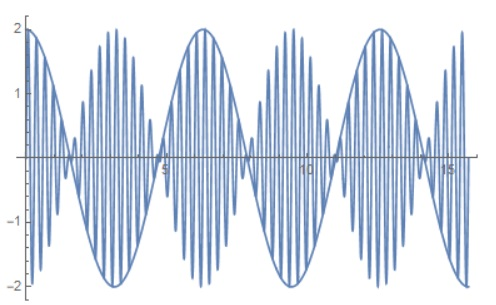
\includegraphics[scale=1]{images/waves/modulation2.jpg}\\
\end{center}
Here, we see that the resultant wave exhibits neither a frequency of 22 Hz nor 20 Hz. Internally, the wave exhibits a frequency of 21 Hz, while overall, the wave moves along with a frequency of 2 Hz. (Notice that this is not simply 1 Hz!) This wave that carries an overall frequency of 2 Hz is called the carrier wave. If we graph $\cos(t)$ directly on top of the function, as shown, this function envelops our combination of two waves perfectly, but it doesn't have the same frequency as the carrier wave - in fact, it has half of the correct frequency. This phenomenon only occurs if the frequencies are sufficiently close enough (and we can hear it in real life if we play a C and a G together, which will sound like an E with a modulating tone beneath that will make it sound like there's a beat within the note). \\
Therefore, when we play two sound waves together, the resultant waves can either mesh together into a single wave and frequency with a modulating frequency determined by a carrier wave, or will noticeably be two separate waves with the same frequencies as before. In each scenario, they will sound different (two tones vs. one tone) based on how close together these frequencies are. 


\section{Double- and Single-Slit Experiments}
This document details the theory behind the single-slit and double-slit experiments as a way to describe how light interferes with itself as it passes through slits. In general, we will consider what happens when we shine light through a set of slits and look at the interference pattern on a screen a distance $D$ away, especially the distances $y$ from the center of the pattern to the locations of minimum/maximum intensity. 

\subsection{Double-Slit Experiment}
We already derived a similar version of this experiment for sound, but we will do it again (and also neglect the spherical nature of the wave).\\
Consider two infinitesimal slits a distance $d$ apart, and a light being shined through these slits. 
\begin{center}
	\begin{asy}
		import graph;
		size(200); 
real wall = 5; 
real D = 9;
real y = 4;
real d = 1.5;
pair sp1 = (0, d); 
pair sp2 = (0, -d); 
draw(Circle(sp1, 0.1)); 
draw(Circle(sp2, 0.1)); 
draw((D, -wall)--(D, wall)); 
draw((0, wall)--sp1+dir(90)*0.2, linetype("4 4")); 
draw((0, -wall)--sp2+dir(270)*0.2, linetype("4 4")); 
draw(sp2+dir(90)*0.2--sp1+dir(270)*0.2, linetype("4 4")); 
dot((D, y)); 
dot((0, 0)); 
draw((0,0)--(D, 0), linetype("4 4")); 
draw((0, -4)--(D, -4), Arrows);
dot((D, 0));
draw((D+0.5, 0)--(D+0.5, y), Arrows); 
draw((-0.5, d)--(-0.5, -d), Arrows);
draw(sp1+dir(25)*0.2--(D, y));
draw(sp2+dir(40)*0.2--(D, y));
draw((0, 0)--(D,y), linetype("8 8")); 

label("$d$", (-0.5, d)--(-0.5, -d), W);
label("$R$", (0,0)--(D,y), dir(140));
label("$y$", (D+0.5, 0)--(D+0.5, y), E);
label("$D$", (0+0.2, -4)--(D-0.2, -4), S);
label("$\theta$", (0,0), dir(12)*7);
	\end{asy}
\end{center}
For some chosen point a distance $y$ from the center, let $R$ be the distance from the midpoint of the slitss to this point, and $\theta$ to be the angle between the line to this point and the perpendicular to the center point. \\
We can compute the wave experienced at this point as the sum of two propagating waves (in exponential form): 
\[
	u(y, t) = \frac{1}{2} \left[ e^{i \left(k \sqrt{D^2 + \left(y - \frac{d}{2} \right)^2} - \omega t\right)} + e^{i \left(k \sqrt{D^2 + \left(y + \frac{d}{2} \right)^2} - \omega t\right)} \right]
\]
Note that taking the imaginary part of this expression will result in the sum of the waves we desire. Since we're mostly concerned where the maximum/minimum intensities are, we can use this exponential form of the wave to describe the wave. We also include the factor of $\frac{1}{2}$ to normalize the wave - it will scale the actual magnitude of the wave down by a factor of $2$, but it will not have an effect on which points will have a maximum/minimum intensity.\\
We will now make the approximation that $D >> d$, and use the Taylor series of the square root term, ignoring terms of second order or higher: 
\begin{align*}
	\sqrt{D^2 + \left(y - \frac{d}{2} \right)^2} &= \sqrt{D^2 + y^2 - yd + \left( \frac{d^2}{4} \right)} \\
	&= R \sqrt{1 - \frac{yd}{R^2} + \frac{d^2}{4R^2}} \\
	&= R \left[1 + \frac{1}{2}\left(\frac{d^2}{4R^2} - \frac{yd}{R^2}\right) - \frac{1}{8}\left(\frac{d^2}{4R^2} - \frac{yd}{R^2}\right)^2 + \ldots \right] \\
	&\approx R\left[1 - \frac{yd}{2R^2} \right] 
\end{align*}
We plug this approximation back into our original expression, using a similar approximation for the other square root: 
\begin{align*}
	u(y, t) &= \frac{1}{2} \left[ e^{i \left(kR - \frac{kyd}{2R} - \omega t\right)} + e^{i \left(k R + \frac{kyd}{2R} - \omega t\right)} \right] \\
	&= \frac{e^{i \left(kR - \omega t\right)}}{2} \left[ e^{- i\frac{kyd}{2R}} + e^{i\frac{kyd}{2R}} \right] \\
	&= e^{i \left(kR - \omega t\right)} \cos \left( \frac{kdy}{2R}\right) = e^{i \left(kR - \omega t\right)} \cos \left( \frac{kd}{2} \sin \theta \right)
\end{align*}
From this, we can see that we can maximize/minimize the amplitude, and thus, the intensity of the sound if we maximize/minimize the cosine term. \\
When the intensity of the sound is observed to be at a maximum, we should have that the argument of the cosine function should be $n \pi$ for some integer $n$ to have a maximum magnitude. This implies:
\[
	\frac{kd}{2}\sin \theta = n \pi  \rightarrow \frac{\pi d}{\lambda}\sin \theta = n \pi \rightarrow d\sin \theta = \lambda n 
\] 
Similarly, when the intensity of the sound is observed to be a minimum, the argument of the cosine function should be $\left( n + \frac{1}{2} \right) n$ for some integer $n$, so the magnitude of the intensity is minimized:
\[
	\frac{kd}{2}\sin \theta = \left( n + \frac{1}{2} \right) \pi  \rightarrow \frac{\pi d}{\lambda}\sin \theta = \left( n + \frac{1}{2} \right) \pi \rightarrow d\sin \theta = \lambda \left( n + \frac{1}{2} \right) 
\]
\subsection{Single-Slit Experiment and Diffraction Gratings}
What happens if the slits are no longer infinitesimal? Let's consider in this case shining light through a single slit of width $a$. By Huygens' Principle, every single point in the slit resembles a point source of light producing a spherical wave. In order to compute this, we consider $N$ infinitesimal slits with distance $d$ between each pair of slits, so $Nd = a$. To clarify our computation, we let $N$ be an odd positive integer (without loss of generality), and index each wave from $\frac{N-1}{2}$ to $-\frac{N-1}{2}$, where the wave indexed at $0$ emanates from the midpoint of the aperture. We also assume that the waves effectively behave as propagating waves rather than spherical waves to simplify calculations. 
\begin{center}
	\begin{asy}
		import graph; 
		size(200); 
		real wall = 5; 
		real D = 7;
		real y = 4;
		real a = 2.5;
		pair sp1 = (0, a); 
		pair sp2 = (0, -a); 
		draw(sp1+dir(180)*0.1--sp1+dir(0)*0.1); 
		draw(sp2+dir(180)*0.1--sp2+dir(0)*0.1); 
		draw((D, -wall)--(D, wall)); 
		draw((0, wall)--sp1); 
		draw((0, -wall)--sp2); 
		draw(sp2+dir(90)*0.2--sp1+dir(270)*0.2, linetype("4 4"));
		dot((0, 0)); 
		draw((0,0)--(D, 0), linetype("4 4")); 
		dot((D, 0)); 
		draw((D+0.5, 0)--(D+0.5, y), Arrows); 
		label("$y$", (D+0.5, 0)--(D+0.5, y), E);
		label("$D$", (0+0.2, -4)--(D-0.2, -4), S);
		dot((D, y)); 
        for (int i = -5; i < 6; ++i)	{
        	draw((D, y)--(0, a/6*i), linetype("2 2")+lightgrey);
        }
        //for (int i = 0; i < 6; ++i)	{
        	//draw(arc((0,0), 0.5+0.2*i, 60, -60));
        //}
		draw((0, -4)--(D, -4), Arrows);
		draw((0, 2)--(D,y), linetype("8 8")); 
		dot((0,2));
		label("$nd$", (-0.5, 2)--(-0.5,0), W);
		draw((-0.5, 2)--(-0.5,0), Arrows);
		draw((-1.5, a)--(-1.5, -a), Arrows);
		label("$a$", (-1.5, a)--(-1.5, -a), W);
		draw((0,0)--(D,y), linetype("8 8"));
		label("$\theta$", (0,0), dir(15)*7);
		label("$R$", (0,0)--(D,y), dir(320));
	\end{asy}
\end{center}
We can compute the waveform of the total wave experienced at a point $y$ from the center by summing up the exponential forms of each of the waves and considering the imaginary part to be our wave. We will normalize the overall wave with a factor of $\frac{1}{N}$. The wave experienced at a point $y$ is then: 
\[
	u(y, t) = \frac{1}{N} \sum_{n = -\frac{N-1}{2}}^{\frac{N-1}{2}} e^{i(k \sqrt{D^2 + (y - nd)^2} - \omega t)}
\]
We first look to simplify the square root. If we define $R = \sqrt{D^2 + y^2}$, and assuming $R >> d$, we can expand the square root using a Taylor series and eliminate second-order terms or higher: 
\begin{align*}
\sqrt{D^2 + (y - nd)^2} &= \sqrt{D^2 + y^2 - 2ndy + n^2d^2}\\
&= R \sqrt{1 - \frac{2ndy}{R^2} + \frac{n^2d^2}{R^2}} \\
&= R \left[1 + \frac{1}{2}\left(\frac{n^2d^2}{R^2} - \frac{2ndy}{R^2} \right) - \frac{1}{8}\left(\frac{n^2d^2}{R^2} - \frac{2ndy}{R^2}  \right)^2 + \ldots \right]\\
&\approx R \left[1 - \frac{ndy}{R^2} \right]
\end{align*}
We can substitute this back in and simplify, pulling out constants: 
\begin{align*}
u(y, t) &\approx \frac{1}{N} \sum_{n = -\frac{N-1}{2}}^{\frac{N-1}{2}} e^{i(kR\left[1 - \frac{ndy}{R^2} \right] - \omega t)} \\
&= \frac{e^{i(kR-\omega t)}}{N} \sum_{n = -\frac{N-1}{2}}^{\frac{N-1}{2}} e^{-i  \frac{kndy}{R}}
\end{align*}
This remaining sum is a geometric series, so we can evaluate it explicitly: 
\begin{align*}
u(y, t) &= \frac{e^{i(kR-\omega t)}}{N} \cdot \frac{e^{i \frac{kdy(N-1)}{2R}} - e^{i\frac{kdy(-N-1)}{2R}}}{1 - e^{-i\frac{kdy}{R}}} \\
&= \frac{e^{i(kR-\omega t)}}{N} \cdot \frac{e^{-i\frac{kdy}{2R}} \left(e^{i \frac{kdyN}{2R}} - e^{-i\frac{kdyN}{2R}} \right)}{e^{-i\frac{kdy}{2R}} \left(e^{i\frac{kdy}{2R}} - e^{-i\frac{kdy}{2R}} \right)} \\
&= \frac{e^{i(kR-\omega t)}}{N} \cdot \frac{2i \sin \left(\frac{kdyN}{2R} \right)}{2i \sin\left(\frac{kdy}{2R}\right)} \\
&= e^{i(kR-\omega t)} \cdot \frac{ \sin \left(\frac{kdyN}{2R} \right)}{N \sin \left(\frac{kdy}{2R}\right)} 
\end{align*}
In order to obtain a function for one slit, we can take the limit as $N \to  \infty$ and $d \to 0$ while holding $a$ constant. We can also take the liberty of substituting $\sin \theta = \frac{y}{R}$, as shown in the diagram:
\[
u(y, t) = \lim_{N \to \infty} e^{i(kR-\omega t)} \cdot \frac{ \sin \left(\frac{ka}{2} \sin \theta \right)}{N \sin \left(\frac{ka}{2N} \sin \theta \right)}
\]
Since $N \to \infty$, it is appropriate to use a small-angle approximation in the denominator and approximate $\sin \phi \approx \phi$ as the argument of the sine function approaches zero:
\[
 u(y, t) = \lim_{N \to \infty} e^{i(kR-\omega t)} \cdot \frac{ \sin \left(\frac{ka}{2} \sin \theta \right)}{N \cdot \frac{ka}{2N} \sin \theta}  \approx e^{i(kR-\omega t)} \cdot \frac{ \sin \left(\frac{ka}{2} \sin \theta \right)}{\frac{ka}{2} \sin \theta} 
\]
If we define $\sinc x = \frac{\sin x}{x}$, we have:
\[
	u(y, t) = e^{i(kR-\omega t)} \sinc \left(\frac{ka}{2} \sin \theta \right)
\]
We will only consider the points of minimum intensity in this waveform. Since intensity is proportional to the square of the amplitude, we have that the intensity will be minimized when $\sinc \left(\frac{ka}{2} \sin \theta \right) = 0$, and therefore:
\[
	\frac{ka}{2} \sin \theta = \pi n \rightarrow \frac{\pi a}{\lambda} \sin \theta = \pi n \rightarrow \frac{a \sin \theta}{n} = \lambda, n \in \ZZ
\]
Points of maximum intensity occur at the maxima of the $\sinc$ function, which are harder to compute (but still doable if we take a derivative, but there is no real nice form for these points). \\
It's worth noting that we can use a similar derivation for diffraction gratings with many slits. Consider our waveform for $N$ slits: 
\[
u(y, t) = e^{i(kR-\omega t)} \cdot \frac{ \sin \left(\frac{kdyN}{2R} \right)}{N \sin \left(\frac{kdy}{2R}\right)} 
\]
If we don't let $d \to 0$ and disregard the width of the grating $a$ while still letting $N \to \infty$, we get that the intensity of the waveform approaches zero in general (as the numerator is bounded between $-1$ and $1$ while $N$ is unbounded). The exception is when $\sin \left(\frac{kdy}{2R}\right)$ is close to zero (or equal to zero), where there exists a nontrivial intensity, since the reciprocal of a very small number is a very large number. This means maxima occur when: 
\[
\frac{kdy}{2R} = \frac{\pi d}{\lambda} \sin \theta = \pi n, n \in \ZZ \rightarrow d \sin \theta = n \lambda, n \in \ZZ
\]
From this, we see that the magnitude of the intensity of the wave, proportional to the amplitude squared, is proportional to the $\sinc$ function squared. The actual experimental single-slit diffraction pattern of a red laser is shown here: 
\begin{center}
	\includegraphics[scale=0.7]{images/waves/singleslitexp.jpg}\\
\end{center}
and the matching graph of the intensity distribution is here: 
\begin{center}
	\includegraphics[scale=1]{images/waves/singleslitwaveform.png}\\
\end{center}
Notice the presence of a large central maximum and dimmer secondary maxima on either side of the center fading into darkness.
\subsection{Double-Slit Experiment Reloaded}
Of course, in reality, when we conduct the double-slit experiment, no matter how hard we pretend, the slits will have some width $a$, however small it may be. Suppose we now set up two slits of non-negligible width a distance $d$ apart and shine a light through these slits.\\
In order to derive the proper waveform for two slits of non-negligible width, we use a similar computation to the situation with a single slit, splitting up the width of the slit into infinitesimal slits and then taking an appropriate limit. Again, we invoke Huygens' Principle, so that every single point in each resembles a point source of light producing a spherical wave (except we neglect the spherical nature of the waves). Just as before, we consider $N$ infinitesimal slits with distance $\delta$ between consecutive infinitesimal slits, holding $N\delta = a$ constant, and assume that $N$ is an odd positive integer. We also use the same indexing scheme for each wave as in the single-slit derivation, letting $n$, a dummy variable, range from $-\frac{N-1}{2}$ to $\frac{N-1}{2}$ and indexing each infinitesimal slit from its distance from the center slit.  
\begin{center}
	\begin{asy}
		import graph; 
		size(200); 
		real wall = 5; 
		real D = 7;
		real y = 4;
		real a = 2.8;
        real d = 0.9; 
		pair s1L = (0, d); 
        pair s1U = (0, a+d);
		pair s2U = (0, -d); 
        pair s2L = (0, -a-d); 
		draw(s1L+dir(180)*0.1--s1L+dir(0)*0.1); 
		draw(s2U+dir(180)*0.1--s2U+dir(0)*0.1); 
        draw(s1U+dir(180)*0.1--s1U+dir(0)*0.1); 
		draw(s2L+dir(180)*0.1--s2L+dir(0)*0.1); 
        draw(s1L+0.1*dir(90)--s1U+0.1*dir(270), linetype("4 4")); 
        draw(s2L+0.1*dir(90)--s2U+0.1*dir(270), linetype("4 4")); 
		draw((D, -wall)--(D, wall)); 
		draw((0, wall)--s1U); 
		draw((0, -wall)--s2L); 
		draw(s2U--s1L);
		dot((0, 0)); 
		draw((0,0)--(D, 0), linetype("4 4")); 
		dot((D, 0)); 
		draw((D+0.5, 0)--(D+0.5, y), Arrows); 
		label("$y$", (D+0.5, 0)--(D+0.5, y), E);
		label("$D$", (0+0.2, -4)--(D-0.2, -4), S);
		dot((D, y)); 
        for (int i = -5; i < 6; ++i)	{
        	draw((D, y)--(0, d+a/2 + a/12*i), linetype("2 2")+lightgrey);
        }
        for (int i = -5; i < 6; ++i)	{
        	draw((D, y)--(0, -d-a/2 + a/12*i), linetype("2 2")+lightgrey);
        }
		draw((0, -4)--(D, -4), Arrows);
		draw((0, 0)--(D,y), linetype("8 8")); 
		draw((-0.5, d)--(-0.5, -d), Arrows);
		label("$d$", (-0.5, d)--(-0.5, -d), W);
        draw((-0.5, d)--(-0.5, a+d), Arrows);
		label("$a$", (-0.5, d)--(-0.5, a+d), W);
        dot((0,-3.2));
        dot((0,-2.3));
		label("$n\delta$", (-0.5, -2.3)--(-0.5, -3.2), W);
		draw((-0.5, -2.3)--(-0.5, -3.2), Arrows);
		draw((0, -3.2)--(D,y), linetype("8 8")); 
		label("$\theta$", (0,0), dir(15)*7);
		label("$R$", (0,0)--(D,y), dir(140));
	\end{asy}
\end{center}
From this setup, we have that the waveform $u(y, t)$ considering $2N$ infinitesimal slits is: 
\[
	u(y, t) = \frac{1}{2N} \left[\sum_{n = -\frac{N-1}{2}}^{\frac{N-1}{2}} e^{i \left(k \sqrt{D^2 + \left(y + \frac{a+d}{2} + n\delta \right)^2} - \omega t \right)} + \sum_{n = -\frac{N-1}{2}}^{\frac{N-1}{2}} e^{i \left(k \sqrt{D^2 + \left(y - \frac{a+d}{2} + n\delta \right)^2} - \omega t \right)} \right]
\]
Just as before, we will use a series of approximations and use a Taylor series expansion to expand the square roots. For simplicity, let's consider the first square root with all positive terms under the square root, as the second square root uses a similar procedure: 
\[
	\sqrt{D^2 + \left(y + \frac{a+d}{2} + n\delta \right)^2} = \sqrt{D^2 + y^2 + \frac{(a+d)^2}{4} + n^2 \delta^2 + 2yn\delta + y(a+d) + n\delta(a+d)}
\]
Just as before, we can factor out $R = \sqrt{D^2 + y^2}$:
\[
	= R\sqrt{1 + \frac{(a+d)^2}{4R^2} + \frac{n^2 \delta^2}{R^2} + \frac{2yn\delta}{R^2} + \frac{y(a+d)}{R^2} + \frac{n\delta(a+d)}{R^2}} \approx R \sqrt{1 + \frac{2yn\delta}{R^2} + \frac{y(a+d)}{R^2}}
\]
where the last step is the throwing out of negligible terms - these being $\frac{n^2 \delta^2}{R^2}$, $\frac{(a+d)^2}{4R^2}$, and $\frac{n\delta(a+d)}{R^2}$, as we assume $a, d, \delta << R$. We can now use the Taylor series expansion of $\sqrt{1+x}$, throwing out all terms after the first two non-zero terms: 
\[
	\approx R \left[1 + \frac{1}{2} \left( \frac{2yn\delta}{R^2} + \frac{y(a+d)}{R^2} \right) \right]
\]
Similarly, we can repeat the same process on the other square root and get: 
\[
	\sqrt{D^2 + \left(y - \frac{a+d}{2} + n\delta \right)^2} \approx R \left[1 + \frac{1}{2} \left( \frac{2yn\delta}{R^2} - \frac{y(a+d)}{R^2} \right) \right]
\]
We can plug back in and factor out the exponential terms that are common to both sums and independent of $n$: 
\begin{align*}
	u(y, t) &\approx \frac{1}{2N} \left[\sum_{n = -\frac{N-1}{2}}^{\frac{N-1}{2}} e^{i \left(k R \left[1 + \frac{1}{2} \left( \frac{2yn\delta}{R^2} + \frac{y(a+d)}{R^2} \right) \right] - \omega t \right)} + \sum_{n = -\frac{N-1}{2}}^{\frac{N-1}{2}} e^{i \left(k R \left[1 + \frac{1}{2} \left( \frac{2yn\delta}{R^2} - \frac{y(a+d)}{R^2} \right) \right]\right)} \right] \\
	&= e^{i(kR-\omega t)} \cdot \frac{1}{2N} \left[\sum_{n = -\frac{N-1}{2}}^{\frac{N-1}{2}} e^{i \left( \frac{kyn\delta}{R} + \frac{ky(a+d)}{2R} \right)} + \sum_{n = -\frac{N-1}{2}}^{\frac{N-1}{2}} e^{i \left( \frac{kyn\delta}{R} - \frac{ky(a+d)}{2R} \right)} \right] \\
	&= e^{i(kR-\omega t)} \cdot \frac{1}{2N}  \left( e^{i \frac{ky(a+d)}{2R}} + e^{-i \frac{ky(a+d)}{2R}} \right) \left[\sum_{n = -\frac{N-1}{2}}^{\frac{N-1}{2}} e^{i \frac{kyn\delta}{R}} \right] \\
	&= e^{i(kR-\omega t)} \cdot \cos\left( \frac{ky(a+d)}{2R} \right) \cdot \frac{1}{N} \left[\sum_{n = -\frac{N-1}{2}}^{\frac{N-1}{2}} e^{i \frac{kyn\delta}{R}} \right] 
\end{align*}
It now suffices to evaluate the remaining geometric series, simplifying as much as possible: 
\begin{align*}
	u(y, t) &= e^{i(kR-\omega t)} \cdot \cos\left( \frac{ky(a+d)}{2R} \right) \cdot \frac{e^{i\frac{ky\delta (1-N)}{2R}} - e^{i\frac{ky\delta (N+1)}{2R}}}{N \left( 1 - e^{i\frac{ky\delta }{R}} \right)} \\
	&= e^{i(kR-\omega t)} \cdot \cos\left( \frac{ky(a+d)}{2R} \right) \cdot \frac{e^{i \frac{ky\delta}{2R}} \left(e^{-i\frac{ky\delta N}{2R}} - e^{i\frac{ky\delta N}{2R}}\right)}{N e^{i\frac{ky\delta }{2R}} \left( e^{-i\frac{ky\delta }{2R}} - e^{i\frac{ky\delta }{2R}} \right)} \\
	&= e^{i(kR-\omega t)} \cdot \cos\left( \frac{ky(a+d)}{2R} \right) \cdot \frac{\sin \left( \frac{ky\delta N}{2R} \right)}{N \sin \left( \frac{ky\delta }{2R} \right)}
\end{align*}
Since $\delta << R$, we can use the small-angle approximation in the denominator $\sin x \approx x$ for sufficiently small values of $x$: 
\begin{align*}
	u(y, t) &\approx e^{i(kR-\omega t)} \cdot \cos\left( \frac{ky(a+d)}{2R} \right) \cdot \frac{\sin \left( \frac{ky\delta N}{2R} \right)}{ \frac{ky\delta N}{2R} } \\
	&= e^{i(kR-\omega t)} \cdot \cos\left( \frac{ky(a+d)}{2R} \right) \cdot \sinc \left( \frac{kya}{2R} \right)
\end{align*}
We can substitute $\frac{y}{R} = \sin \theta$, which gives:
\[
	u(y, t) = e^{i(kR-\omega t)} \cdot \cos\left( \frac{k(a+d)}{2} \sin \theta \right) \cdot \sinc \left( \frac{ka}{2} \sin \theta \right)
\]
Notice that the waveform is a product of the double-infinitesimal-slit waveform derived in the first section and the single-slit waveform derived in the section. This implies that the consideration of a non-negligible slit width simply superposes the single-slit distribution on top of the double-slit distribution. We can see this through an actual experiment: 
\begin{center}
	\includegraphics[scale=0.7]{images/waves/doubleslitexp.jpg}\\
\end{center}
or by means of graphing the intensity (which is proportional to amplitude squared): 
\begin{center}	
\includegraphics[scale=0.7]{images/waves/doubleslitwaveform.png}\\
\end{center}
As one can see from the graph and the experiment, the double-slit result is simply the result of the overlaying of the infinitesimal double-slit pattern (uniform, closely spaced peaks of intensity) and the single slit pattern (fading, large maxima out from the center). 

\part{Mechanics, Non-Electric Boogaloo}

\section{Mathematics Excursion III: Lagrange Multipliers and Extrema}

This is a lecture on the method of Lagrange multipliers, which essentially discusses optimization subject to constraints. We will use this perspective when discussing Lagrangian mechanics, so it's highly advised that one at least reads this particular set of notes through. In single-variable calculus, it's well-known how to optimize a function of a single variable, but this handout discusses how to do so with multiple variables, and with constraints imposed. 

\subsection{Extrema of Functions of Multiple Variables}
For this section, to begin with, we only discuss functions of two variables for visualization and simplicity. Of course, the techniques used here can be generalized easily. 

The most natural way to generalize the notion of a critical point for a function of multiple variables is by assuming \textit{all partial derivatives of a function $f$ with respect to all of its independent variables} at a critical point are zero or undefined, of which a function of only one variable gives us  a special case for this. This can equivalently be thought of saying that the gradient of this function, $\grad f$, is zero or undefined, which has some useful geometric intuition behind it. 

We can classify critical points based on the second derivatives of the variables. At a critical point, if the second (partial) derivatives of the function with respect to $x$ and $y$ are both positive, the function achieves a minimum, and similarly, if the second derivatives with respect to $x$ and $y$ are both negative, the function achieves a maximum. If one is positive and one is negative, we have what we call a \textit{saddle point}, which looks aptly like a saddle. This notion generalizes to functions of three or more variables, but obviously we can't see them as visually as we do here. 
\begin{figure}[h!]
\centering
\begin{minipage}{0.3\textwidth}
\centering
\includegraphics[scale=0.2]{images/math/multivar/localmax.png}
\end{minipage}
\begin{minipage}{0.3\textwidth}
\centering
\includegraphics[scale=0.2]{images/math/multivar/localmin.png}
\end{minipage}
\begin{minipage}{0.3\textwidth}
\centering
\includegraphics[scale=0.2]{images/math/multivar/saddlepoint2.png}
\end{minipage}
\end{figure}

%A theorem that we will now state for all multivariate functions, but not prove, is that on an open region, if a function is known to achieve a maximum or minimum value on the region, then it must do so at a critical point. 

\subsection{Optimizing with a Constraint}
Suppose now we want to optimize a function of two or more variables, but now subject to a constraint. Let's do an actual example for clarity: 
\begin{problem}
Find the maximum value of $x^3y$ on the ellipse $3x^2+2y^2 = 12$. 
\end{problem}
We can interpret this geometrically, first by considering the \textit{level curves} of the function we're studying (in this case, $f(x, y) = x^3y$), which are the curves of constant $f$. If we were to draw them out on top of the the ellipse on the plane, we can see that some sort of critical point should be reached when a level curve is tangent to the ellipse. If we think of the value of our constraint as a varying function $g(x, y) = 3x^2 + 2y^2$ that is forced to take on some value, this intuition tells us the gradients of these functions at this critical point should be parallel, ie. $\grad f = \lambda \grad g$ for some real $\lambda$. We call $\lambda$ the \textit{Lagrange multiplier} associated with $g$. Once we get the conditions associated with these parallel vectors, we can re-impose our constraint with $g$, and then get the desired maximum and the point at which the maximum is achieved. 

We could carry out the computation in this way, but we'll instead shift to a mostly algebraic/abstract way to do this that's equivalent. We'll incorporate the constraints and the function we're studying and roll them up into one function, what's sometimes called the \textit{Lagrangian function}. If our function of interest is $f$, and our constraints are $g$, we consider
\[
	\lagr(x, y) = f(x,y) + \lambda g(x, y).
\]
Conventionally, $g$ should be written in a form that should be equal to 0 when it is satisfied. We will take partial derivatives of $\lagr$ with respect to every independent variable and set them equal to 0 -- in this case, that would be $x$, $y$, and also $\lambda$. The partial derivative with respect to our Lagrange multiplier just gives back the constraint, and the other two equations will give a system of equations to solve. This will give us the proper critical points that we want. 

Let's actually do this example for real - let $\lagr(x, y) = x^3y - \lambda(3x^2 + 2y^2 -12)$, giving 
\[
	\lagr_x = 3x^2 y - 6 \lambda x = 0 \quad \lagr_y = x^3 - 4 \lambda y = 0 \quad \lagr_\lambda = 3x^2 + 2y^2 - 12 = 0 
\]
We more or less ignore the last equation until we use it as the constraint that needs to be satisfied, and we mess with the first two equations: 
\[
	6x^2 y^2 - 12\lambda x y - (3x^4 - 12 \lambda x y) = 3x^2(2y^2 - x^2) = 0
\]
Either $x = 0$, or from the constraint, $x^2 = 2y^2$ so $x = \pm \sqrt{3}$. We can now plug in each of these critical values of $x$ to see which one maximizes $x^3y$ (and by inspection, it's the value $x = \sqrt{3}$ with $y = \sqrt{\frac{3}{2}}$ that gives $\frac{9}{\sqrt{2}}$).
Notice that this latter perspective is much more generalizable, as it admits as many constraints. If we have $n$ constraints, each of which is a function $g_k$, we will instead consider the Lagrangian function 
\[
	\lagr(x, y) = f(x,y) + \sum_{k=1}^n \lambda_k g_k(x, y)
\]
and perform the same operations. 

The topic of Lagrangian multipliers and constrained optimization is important, and it will come up again when we discuss the Lagrangian method. 


\section{Mathematics Excursion IV: Variational Calculus}

This lecture is a prelude to the following lectures that will be focused on the Lagrangian approach to mechanics, an approach that is not only equally valid but also sometimes more convenient in some scenarios to describe a system that produces the same results with perhaps some different insights. To really get into the subject, we have to introduce a little bit of additional mathematics that is necessary to understand the Lagrangian method. 

\subsection{The Euler-Lagrange Equation}
The calculus of variations is interested mostly in objects called functionals $F$, where $F: f \rightarrow \RR$ mapping functions to reals. We will be especially interested in functionals $F[y]$ of the form
\[
	F[y] = \int_{x_1}^{x_2} f(x, y, y') \, dx 
\]
for some choice of the inside function $f$. We will often look to extremize the value of this functional by an appropriate choice of a function $y$ such that $F[f]$ is a stationary point, implying that this function maximizes or minimizes the functional, but it could also be a saddle point. We don't have a good intuition for what it means for a functional to have a stationary point at a function, so we'd like to parameterize this in terms of a scalar that we can actually do regular calculus on. 

Suppose our function $y$ produces a stationary value of $F[y]$. For any small $0 \leq \epsilon \ll 1$ and a differentiable non-zero function $\xi$ such that $\xi(x_1) = \xi(x_2) = 0$, we can consider the functional $F[y + \epsilon \xi]$. Notice that we could effectively interpret this as fixing $\xi$ and making the functional solely as a function of $\epsilon$, defining 
\[
	\tilde{F}(\epsilon) = F[y + \epsilon \xi] = F[q]
\]
and letting $q = y + \epsilon \xi$ for brevity. Notice that at $\epsilon = 0$, we have $\tilde{F}(\epsilon) = F[y]$, so $\epsilon = 0$ is a stationary point of $\tilde{F}$.  

It would be nice for us to figure out a relation involving $y$ to our choice of $f$ to find the stationary points of $F[y]$. We can consider expanding $\dv{\tilde{F}}{\epsilon}$ by moving the derivative inside the integral and applying the chain rule. We will find that the term $\dv{x}{\epsilon} = 0$, since $x$ is simply the dummy variable of integration, and the terms $\dv{q}{\epsilon}$ and $\dv{q'}{\epsilon}$ will be $\xi$ and $\xi'$ by our definition of $q$. When we compute this derivative, we will get 
\begin{align*}
\dv{\tilde{F}}{\epsilon} &= \dv{}{\epsilon} \int_{x_1}^{x_2} f(x, y + \epsilon \xi, y' + \epsilon \xi') \, dx \\
&= \int_{x_1}^{x_2} \left(\pdv{f}{x} \dv{x}{\epsilon} + \pdv{f}{q} \dv{q}{\epsilon} + \pdv{f}{q'} \dv{q'}{\epsilon} \right) \, dx \\
&= \int_{x_1}^{x_2} \left(\pdv{f}{q}\xi + \pdv{f}{q'} \xi' \right) \, dx.
\end{align*}
We now "integrate by parts", by using the product rule in reverse: 
\begin{align*}
	&= \int_{x_1}^{x_2} \left(\pdv{f}{q}\xi + \dv{}{x}\left(\pdv{f}{q'}\xi \right) - \xi \dv{}{x} \pdv{f}{q'}\right) \, dx  
\end{align*}
At $\epsilon = 0$, we have $\dv{\tilde{F}}{\epsilon} = 0$, so we now plug in $\epsilon = 0$ to obtain
\begin{align*}
	0 &= \int_{x_1}^{x_2} \xi\left(\pdv{f}{y} - \dv{}{x} \pdv{f}{y'}\right) \, dx + \pdv{f}{y'}\xi \Big|_{x_1}^{x_2} \\
	&= \int_{x_1}^{x_2} \xi\left(\pdv{f}{y} - \dv{}{x} \pdv{f}{y'}\right) \, dx 
\end{align*}
where the last term vanishes because of our boundary conditions. 

We will now use the \textbf{fundamental lemma of the calculus of variations}, which states that if for continuous functions $g$ and $h$ on an open interval $(a, b)$ such that $h \neq 0$ and $h$ vanishes everywhere outside $(a,b)$, we have
\[
	\int_a^b g(x)h(x) \, dx = 0
\]
then $g(x) = 0$. 

Applying this gives the expression in parentheses is zero, so that
\[
	\pdv{f}{y} - \dv{}{x} \pdv{f}{y'} = 0.
\]
This is the \textbf{Euler-Lagrange equation}, called Euler's differential equation in the mathematical literature, and we will be seeing it frequently when discussing Lagrangian mechanics. This relation \textit{must} be true if $y$ extremizes the functional $F[y]$. 

This generalizes to if we have multiple independent variables dependent on $x$, in which case we can apply the same analysis to each of these individual variables. That being said, we then essentially require the Euler-Lagrange equation to hold true for every single one of those independent variables, independently of one another. 

Another useful equation that captures the same information as the Euler-Lagrange Equation is Euler's integral equation, which essentially combines this with the chain rule on $f$:
\[
	\dv{f}{x} = \pdv{f}{x} + \pdv{f}{y}\dv{y}{x} + \pdv{f}{y'}\dv{y'}{x}
\]
Notice also that 
\[
	\dv{}{x}\left(y' \pdv{f}{y'} \right) = \pdv{f}{y'} \dv{y'}{x} + y' \dv{}{x} \pdv{f}{y'} 
\]
and with a bit of substitution we have 
\[
	\dv{}{x}\left(y' \pdv{f}{y'} \right) = \dv{f}{x} - \pdv{f}{x} - \pdv{f}{y}\dv{y}{x} + y' \dv{}{x} \pdv{f}{y'} = \dv{f}{x} - \pdv{f}{x} + y'\left(\dv{}{x} \pdv{f}{y'} - \pdv{f}{y}\right)
\]
By Euler-Lagrange, the last term vanishes, and if $y$ has no explicit dependence on $x$, we obtain that 
\[
	\dv{}{x} \left( f - y' \pdv{f}{y'} \right) = 0
\]
or, Euler's integral equation that states 
\[
	 f - y' \pdv{f}{y'} = C
\]
for some arbitrary constant $C$.

\subsection{Constraints}
Introducing constraints into the system fixes relationships between our independent variables, which makes them correlated in some way. That is very sad, because then our previous argument of having all of the Euler-Lagrange equations for all the variables be satisfied simultaneously is on weak ground, since we argued all the variables had to be independent. Constraints also can be extremely sad, depending on what we say about the system - if the constraint can be described using an algebraic equation, then we are a bit happier and we call this constraint \textit{holonomic}. If not, obviously, we call them non-holonomic and we continue to be very sad. For example, if we confine a particle to a sphere or a surface of a ball, this is holonomic as it is described by $x^2 + y^2 + z^2 = R^2$, where $R$ is the radius of the ball - if we say instead that a particle can move around inside the ball, this is non-holonomic as now $x^2 + y^2 + z^2 \leq R^2$. Of course, these constraints  can be regular algebraic expressions, or they can be differential equations or integral expressions that must also be satisfied. Other words you might hear describing the nature of constraints: if a constraint is time-dependent, it is called \textit{rheonomic}, in contrast to being \textit{scleronomic} if it is not. 

Constraints can be dealt with in many different ways. The physical way to do it is to introduce \textit{generalized coordinates} - that is, bake the constraints into the independent coordinates you are using for the system. For example, if we have a constraint normal force on a system, we can choose a coordinate perpendicular to the normal force so that it does no work, thus eliminating that constraint explicitly. 

%Another way to do this is with the Lagrange multipliers method, which works by considering \textit{variations} of the functional $F$ when $F$ is stationary, and tacks on the constraints. When extremized, if $F$ is displaced virtually by $\delta F$, we can express this variation in terms of virtual displacements of the $n$ coordinates: 
%\[
%	\delta F = \sum_i^n \pdv{F}{q_i} \delta q_i
%\]
%If we also have $m$ holonomic constraints, when $F$ is varied, we 
\subsection{Examples} 
\subsubsection{The Path With The Shortest Distance Between Two Points Is...}
\begin{problem}
Suppose we have two points, labeled $1$ and $2$, on a Cartesian plane. Find the path that minimizes the distance between these two points. 
\end{problem}

\begin{solution}
We will do this variationally. Let $y$ be the desired minimal path. Note that the infinitesimal arc length of the path, $ds$, is given by $\sqrt{dx^2 + dy^2} = \sqrt{1 + \left(\dv{y}{x}\right)^2} \, dx$, so it suffices to minimize the integral functional
\[
	L = \int_1^2 \sqrt{1 + \left(\dv{y}{x}\right)^2} \, dx = \int_1^2 \sqrt{1 + y'^2} \, dx.
\]
Applying Euler-Lagrange, we see no explicit dependence on $y$, so we get that 
\[
	\dv{}{x} \frac{y'}{\sqrt{1+y'^2}} = 0 \implies
	\frac{y'}{\sqrt{1+y'^2}}  = C
\]
for some real $C$. Rearranging, we get 
\[
	y'^2 = a
\]
for some (other) real constant, so $\dv{y}{x}$ is a constant. That means that $y$ must be a line, as known by Euclid some millenia ago. 
\end{solution}

\subsubsection{The Brachistocrone Problem}
\begin{problem}
Find the shape of the path that minimizes the transit time between two points at different elevations under the influence of a uniform gravitational field.
\end{problem}

\begin{solution}
Let us set our potential to be zero at the top of our path, where we also set $y = 0$. By conservation of energy, we have the velocity at any given elevation to be $v = \sqrt{2gy}$. Thus, the total transit time $T$ is computed by integrating over the entire length of the path: 
\[
	T = \int_1^2 \frac{ds}{v} = \int_1^2 \sqrt{\frac{dx^2 + dy^2}{2gy}} = \int_1^2 \sqrt{\frac{x'^2  + 1}{2gy}} \, dy 
\]
Since the constant $\frac{1}{\sqrt{2g}}$ just comes out of the integral, we are only concerned with using Euler-Lagrange on $f(x, y) = \sqrt{\frac{x'^2  + 1}{y}}$. Notice that $\pdv{f}{x} = 0$, so we can integrate to get
\[
	\frac{x'}{\sqrt{y(1 + x'^2)}} = C
\]
for some constant $C$. With some foresight and rearrangement, we can replace the constants enough so that we get 
\[
	x' = \frac{y}{\sqrt{2ay-y^2}}
\]
To integrate this, we consider the substitution $y = a(1-\cos\theta)$, which yields a lot of cancellations and gives $x = a(\theta - \sin \theta)$. This result can be interpreted as the curve traced when a circle rolls across a flat surface, which is called a \textit{cycloid}. For reference, a sketch of the curve is given below: 
\begin{center}
\includegraphics[scale=0.3]{images/mechadv/cycloid.png}
\end{center}

\end{solution}

\subsection{Exercises}
\begin{enumerate}
\item Find and describe the path $y = y(x)$ for which the integral 
\[
	\int_{x_1}^{x_2} \sqrt{x} \sqrt{1 + y'^2} \, dx 
\]
is stationary. 

\item This problem concerns the \textit{catenary}, a shape formed when a uniform rope of fixed length hangs under the force of gravity. Show that, by minimizing the gravitational potential energy and constraining the length to be fixed, the rope takes the shape of a $\cosh$ curve, that is, a hyperbolic cosine curve. 

\item Find the minimal surface between two circles of radius $R$ with centers aligned along the $z$-axis, with a distance of $h$ between them. Choose your independent variables and coordinate systems wisely. Does the solution look familiar? 

\item This concerns the time traveled between two points on a cycloid. A cycloid is traced out by a point on a circle of radius $a$ as the circle rolls without slipping for one revolution. Suppose a mass is released from rest at any point $P_0$ associated with angle $\theta_0$, $0 < \theta_0 < \pi$, on the track between the highest point $O$ and the lowest point $P$. Compute the time it takes for the mass to reach $P$ as the integral 
\[
	\sqrt{\frac{a}{g}} \int_{\theta_0}^\pi \sqrt{\frac{1-\cos\theta}{\cos\theta_0 - \cos \theta}} \, d\theta 
\]
and evaluate this integral as $\pi \sqrt{\frac{a}{g}}$.

\item Find the dimensions of the parallelopiped of maximum volume circumscribed by a sphere of radius $R$. 


\end{enumerate}

\section{Lagrangian Mechanics}
This is out first real look at Lagrangian mechanics, where we will start from Newton's Second Law and things we already know and derive an expression that may look familiar to one acquainted with some variational calculus. The new framework we will develop will force us to adopt a differing, but equivalent perspective on how nature works and change how we see mechanics.

%\subsection{Motivating the Lagrangian} %clarity in this section is INFALLIBLY IMPORTANT

%alternative interpretion of nature to minimize a quantity (a FUNCTIONAL) called the action that depends on the path (potentials) and motion (kinetic) of a particle => allowing us to use the Euler-Lagrange eqns. Then, from d'Alembert's principle and also wanting to get rid of vector quantities (and remove our grievances with Newtonian), showing that K-V is a good choice that satisfies the Euler-Lagrange eqns. 

Before we move into the Lagrangian system, we'd like to hear some complaints about the Newtonian system, and what we might want to see in our new and improved system: 
\begin{enumerate}
\item \textbf{Too many equations of motion.} For any body, we have $6$ equations of motion per body that succinctly show the acceleration of that object. That's fine, but these equations of motion are often coupled second-order differential equations if things get messy and with more and more objects. Thermodynamics offers an alternative solution to this problem in the case of many, many particles if all we are concerned with is energy, but we would like to be able to actually \textit{look at} how all these objects move. 

\item \textbf{Vectors are hard to deal with in general coordinate systems.} They work best if we stick to exclusively one coordinate system (maybe Cartesian), but moving vectors between representations in polar/cylindrical/spherical/rectangular/whatever other coordinates we might find useful is a pain and can be very messy. Scalar quantities, such as energy, do not suffer from this barrier - so we might be motivated to look at scalar quantities such as energy to help us out...

\item \textbf{Finding and accounting for forces, including fictional forces and constraint forces.} It's paramount to account for all possible forces on a system when applying Newton's Second Law. However, depending on your choice of reference frame, we may have to include fictional forces to account for motion that appears to come from nowhere at all. Furthermore, from Newton's Third Law, interactions between objects have contact forces that may behave in ways that can be very complicated and influence the motion of objects in weird ways. In general, while forces are a useful tool for visualizing the interactions between objects in a system intuitively, the motion of the objects can be lost if we do not do this correctly.
\end{enumerate}

With this in mind, and the fact that we have some new mathematics under our belts, let us work from a slight modification of what we know already about mechanics, ie. Newton's Second Law, and slowly develop the Lagrangian method.

Before physicists developed a suitable theory for dynamical systems, Bernoulli had already given statics a variational perspective. Consider a system of $N$ particles in equilibrium, so the total force on each particle $i$ is $0$, where $i$ can be an index from $1$ to $N$. Let the net force on particle $i$ be $\vec F_i$. One of the sneaky ideas we can use is to give each force a virtual displacement $\delta\vec r_i$ on each particle, that is, we allow the particles to shift by a slight, infinitesimal amount, without evolving the system in time. The quantity $\vec F_i \cdot \delta \vec r_i$ is called, appropriately, the \textit{virtual work.} Because the system is in equilibrium, the total virtual work must obviously be 0. From a Newtonian perspective, by summing over all the particles, then, we can write 
\[
	\sum_i^N \vec F_i \cdot \delta \vec r_i = 0. 
\]
We can decompose these forces into applied forces on these particles, $\vec F_i^A$, and constraint forces, $\vec F_i^C$. These sets of forces can be chosen in a way that is convenient to us, and we can separate them - 
\[
	\sum_i^N \vec F_i^A \cdot \delta \vec r_i + \sum_i^N \vec F_i^C \cdot \delta \vec r_i = 0.
\]
The second sum can be ignored if no virtual work is done by the constraint forces. This is true if the virtual displacements are tangent to a surface that the particle moves along, and the constraint force are normal to them, or alternatively if we are working with a rigid body. If we ignore this, we arrive at Bernoulli's Principle of Static Virtual Work: 
\[
	\sum_i^N \vec F_i^A \cdot \delta \vec r_i = 0
\]
That's fine and good, but in a dynamical system, things are moving according to Newton's Second Law - which, as a reminder, is 
\[
	\vec F = \dv{\vec p}{t} = \dot{\vec p} \implies \vec F - \dot{\vec p} = 0.
\]
Repeating this analysis with moving objects, we have to account for the movement of these objects through their momentum, $\vec p_i$, in order to obtain zero virtual work. Thus, with an analogous analysis, we arrive at \textit{d'Alembert's Principle}, 
\[
	\sum_i^N (\vec F_i^A - \dot{\vec {p_i}}) \cdot \delta \vec r_i = 0
\]

Recall in our discussion last week that we could break down systems into $N$ independent generalized coordinates $q_j$ that allow us to skirt around these constraint forces. This means each of the variations of these coordinates, $\delta q_j$, are independent, and we can break it down as such with the chain rule:
\[
	\delta \vec r_i = \sum_j^N \pdv{\vec r_i}{q_j} \delta q_j
\]	
We can similarly express the velocity of a particle in these coordinates, but now we must include a temporal term, as this is no longer virtual: 
\[
 \dot{\vec{r_i}} = \dv{\vec r_i}{t} = \sum_j^N \pdv{\vec r_i}{q_j} \dv{q_j}{t} + \pdv{\vec r_i}{t} = \sum_j^N \pdv{\vec r_i}{q_j} \dot q_j + \pdv{\vec r_i}{t} 
\]
With this, we can break d'Alembert's Principle into contributions based on variations of coordinates. We look first at the contributions from the applied force terms: 
\[
	\sum_i^N \vec F_i^A \cdot \delta \vec r_i = \sum_i^N \sum_j^N \left(F_i^A \cdot \pdv{\vec r_i}{q_j} \right) \delta q_j = \sum_j^N Q_j \delta q_j.
\]
We have organized these terms into components of the \textit{generalized force} $Q_j$, where each component $Q_j$ is defined as 
\[
	Q_j = \sum_i^N F_i^A \cdot \pdv{\vec r_i}{q_j}.
\]
Now, let's look at the momentum terms, and see if we can coax it in to a form that is favorable to us. We're going to "reverse-product rule", applying Clairaut whenever we can to put things in terms of derivatives in $q_j$, and rearrange terms until we can either recognize something familiar.
\begin{align*}
	\sum_i^N \dot{\vec{p_i}} \cdot \delta \vec r_i &= \sum_i^N \sum_j^N \left( m \ddot{\vec {r_i}} \cdot \pdv{\vec r_i}{q_j} \right) \delta q_j  = \sum_i^N \sum_j^N \left[ m\dv{}{t} \left(\dot{\vec{r_i}} \cdot \pdv{\vec r_i}{q_j} \right) - m \dot{\vec{r_i}} \cdot \pdv{\dot{\vec {r_i}}}{q_j} \right]\delta q_j \\
	&= \sum_i^N \sum_j^N \left[m \dv{}{t} \left(\dot{\vec{r_i}}  \cdot \pdv{\dot{\vec{r_i}}}{\dot{q_j}} \right)  - m \dot{\vec{r_i}} \cdot \pdv{\dot{\vec{r_i}}}{q_j} \right] \delta q_j 
\end{align*}
Notice that $\pdv{\dot{\vec{r_i}}}{\dot{q_j}} = \pdv{\vec r_i}{q_j}$, so we can substitute:
\begin{align*}
\sum_i^N \sum_j^N \left[m \dv{}{t} \left(\dot{\vec{r_i}}  \cdot \pdv{\dot{\vec{r_i}}}{\dot{q_j}} \right)  - m \dot{\vec{r_i}} \cdot \pdv{\dot{\vec{r_i}}}{q_j} \right] \delta q_j 
	&= \sum_i^N \sum_j^N \left[m \dv{}{t} \left( \frac{1}{2} \pdv{\dot{r_i}^2}{\dot{q_j}} \right)  - m \frac{1}{2} \pdv{\dot{r_i}^2}{q_j} \right] \delta q_j  \\
	&=  \sum_j^N \left[ \dv{}{t} \left( \pdv{K}{\dot{q_j}} \right) - \pdv{K}{q_j} \right] \delta q_j 
\end{align*}
where $K$ here is the total kinetic energy. 

Plugging back into d'Alembert's Principle, we now only have stuff dependent on the coordinates $q_j$:
\[
	\sum_j^N \left(Q_j - \dv{}{t} \left( \pdv{K}{\dot{q_j}} \right) + \pdv{K}{q_j} \right) \delta q_j = 0
\]
We can split the generalized force into a conservative component, which is the negative gradient of some potential $V$, and an extra part consisting of non-conservative, velocity dependent, or other constraint forces, $Q^{EX}$: 
\[
	Q = -\grad V + Q^{EX}
\]
Again, we break this down along coordinates, and we have
\[
	\sum_j^N \left(-\pdv{V}{q_j} + Q^{EX}_j - \dv{}{t} \left( \pdv{K}{\dot{q_j}} \right) + \pdv{K}{q_j} \right) \delta q_j = 0
\]
Combining terms and flipping the overall sign, we have
\[
\sum_j^N \left(\dv{}{t} \left( \pdv{K}{\dot{q_j}} \right) + \pdv{(K-V)}{q_j} - Q^{EX}_j \right) \delta q_j = 0
\]
Since the potential is only dependent on position, we can add zero to this sum without changing its value. Let's add the fairly contrived term $\sum_j^N \dv{}{t} \left(\pdv{V}{\dot{q_j}}  \right) \delta q_j $, which is zero because mechanical potential energies do not depend on the time-derivatives of the coordinates. Therefore, we have: 
\[
\sum_j^N \left(\dv{}{t} \left( \pdv{(K-V)}{\dot{q_j}} \right) + \pdv{(K-V)}{q_j} - Q^{EX}_j \right) \delta q_j = 0
\]
Each of these terms must be zero independently of one another, so we have
\[
	\dv{}{t}\pdv{(K-V)}{\dot{q_j}} - \pdv{(K-V)}{q_j} = Q^{EX}_j 
\]
and if we assume that no contributions are from those extra forces, we have
\[
\dv{}{t}\pdv{(K-V)}{\dot{q_j}} - \pdv{(K-V)}{q_j} = 0 
\]
But wait... that looks like Euler-Lagrange! In fact, we have now shown that if we let $\lagr = K - V$ in nice systems, we get the Euler-Lagrange equations to show up instead of Newton's Laws for an equally valid formulation of mechanics. We call $\lagr$ the \textit{Lagrangian}. We can now apply Euler-Lagrange to get the equations of motion of the system directly without much free-body diagram work. Thus, we have successfully constructed a new framework for mechanics involving energy and without vector quantities explicitly woven into it (ie. forces). We also don't need to be worried about constraints, because we can choose what our coordinates are, as long as they are independent. That's pretty nice! 

A sidenote -- we can also introduce additional constraints with the Lagrange multipliers method, which allows us to put in extra holonomic constraints on the system that can't necessarily be wrapped up in some variable. If we introduce these terms, the full Euler-Lagrange equation looks more like 
\[
	\dv{}{t}\pdv{\lagr}{\dot{q_j}} - \pdv{\lagr}{q_j} = \sum_{k=1}^r \lambda_k \pdv{g_k}{q_j} + Q^{EXC}_j
\]
where the $g_k$ are the extra constraints and the $\lambda_k$ are the Lagrange multipliers associated with them. Now, the additional generalized force term $Q^{EXC}_j$ is limited to all the extra forces that are non-conservative or are velocity-dependent. 

Seeing that the Euler-Lagrange equations are satisfied, given our variational calculus knowledge from last time, we are led to define a quantity called the \textbf{action} $S$ of the system on a time interval $[t_1, t_2]$, a functional that integrates our Lagrangian, a function of $N$ generalized coordinates, from $t_1$ to $t_2$: 
\[
	S[\mathbf q] = \int_{t_1}^{t_2} \lagr(t, \mathbf q, \dot{\mathbf q}) \, dt
\]
As the Euler-Lagrange equations are true, we thus must have the first variation of the action be zero, or 
\[
	\delta S = \delta \int_{t_1}^{t_2} \lagr(t, \mathbf q, \dot{\mathbf q}) \, dt = 0.
\]
This is the \textbf{principle of stationary action}, implying that nature tends to minimize this energy-related quantity or make it take on extremal values. This idea can be motivated to some extent from optics, and noting that light moves in such a way to minimize its path length and time taken to travel. Philosophically, this is a different perspective than Newtonian mechanics, which is based around inertial frames and stating how objects move subject to forces. 



\section{Noether's Theorem and Hamiltonian Mechanics}
One of the most important tools that we were able to use when solving problems before was with conserved quantities, such as linear momentum, angular momentum, and energy - but it's not really clear how they arise in Lagrangian mechanics. This section will serve to persuade you that not only do they arise naturally, but the manner in which they manifest themselves is on a much deeper level than we could have bargained for. 

First, let's define a more general form of momentum - for a coordinate $q_i$, the \textit{generalized momentum} for that coordinate is the quantity $p_i = \pdv{\lagr}{\dot{q_i}}$. If we plug this into the Euler-Lagrange equation:
\[
	\dv{p_i}{t} = \pdv{\lagr}{q_j} + \sum_{k=1}^r \lambda_k \pdv{g_k}{q_j} + Q^{EXC}_j
\]
Notice that if the Lagrangian does not explicitly depend on the coordinate $q_i$, and if there are no contributions from the constraints and other forces, the equation reduces dramatically: 
\[
	\dv{}{t}p_i = \dot{p_i} = 0
\]
In this case, $p_i$ is a constant of motion. If the Lagrangian was to not be dependent on $q_i$, we say the Lagrangian is \textit{spatially homogeneous} with respect to $q_i$, and we call $q_i$ a \textit{cyclic coordinate}. As a simple example, we can look at the case of a free particle not under the influence of any potential in Cartesian coordinates:
\[
	\lagr = \frac{1}{2} m v^2 = \frac{1}{2} m ( \dot{x}^2 + \dot{y}^2 + \dot{z}^2 )
\]
If we apply Euler-Lagrange to $x$, for example: 
\[
	\dv{}{t}\pdv{\lagr}{\dot{x}} = \dv{}{t} (m \dot{x}) = \pdv{\lagr}{x} = 0 
\]
and a similar result holds for $y$ and $z$. Notice that in the absence of a potential, no external forces are acting on the object - therefore, in the absence of an external force, we have  $p_x = m \dot {x}$ to be a constant, which you might recognize as the linear momentum in the $x$-direction. In general, the entire vector $m \dot{\vec{r}}$ is a constant, so we get conservation of linear momentum for free! We can similarly get conservation of angular momentum if we apply the same idea to a freely rotating particle and use cylindrical/spherical coordinates. 

This, in essence, is \textbf{Noether's Theorem}, which states that if the Lagrangian is independent of some coordinate, then there exists a conserved quantity corresponding to it. This implies that we can shift the coordinate (by a first-order term) however we want, and we'll still have the conserved quantity. Back to our free-particle example, this is like saying that no matter where you put your origin on the $x$-axis, the particle will still have its $x$-linear momentum conserved. 

In general, if we can shift the values of the coordinates so that the Lagrangian is invariant (i.e. perform an \textit{invariant transformation}), we actually will still have a conserved quantity. The proof of this follows from some explicit mathematical computation. For any symmetry, by definition, the Lagrangian is constant, so we have $\dv{\lagr}{\epsilon} = 0$: 
\begin{align*}
	0 = \dv{\lagr}{\epsilon} &= \sum_i \left[\pdv{\lagr}{q_i} \dv{q_i}{\epsilon} + \pdv{\lagr}{\dot{q_i}} \dv{\dot{q_i}}{\epsilon} \right] \\
	&= \sum_i \left[\dv{}{t} \left(\pdv{\lagr}{\dot{q_i}} \right)\xi_i + \pdv{\lagr}{\dot{q_i}}\dot{\xi_i}  \right] \\ 
	&= \dv{}{t} \sum_i \left(\pdv{\lagr}{\dot{q_i}} \xi_i \right) = \dv{}{t} \sum_i p_i \xi_i = \dv{}{t}(\mathbf{p} \cdot \mathbf{\xi})
\end{align*}
where $\mathbf{p} = (p_1, p_2, \ldots, p_n)$ and a similar definition for $\mathbf{\xi}$ - both of which are vectors. This last expression, $\mathbf{p} \cdot \mathbf{\xi}$, is called the conserved momentum for this invariant transformation. 

\subsection{The Hamiltonian and the Generalized Energy Theorem}
How do we get to the idea of conservation of energy? The only coordinate that we haven't really talked about homogeneity with is the time coordinate $t$, and so it makes sense that energy is the conserved quantity associated with temporal invariance. However, time is special when discussing symmetries, because we can vary our coordinates, but we can't really discuss varying time. In order to investigate this, we start by considering the total time derivative of the Lagrangian: \footnote{Assume, for the sake of our results and for the rest of the handout, that we don't have any constraints lying about, and neither do we have weird, non-conservative, velocity-dependent forces, so we don't have the extra terms that come with Euler-Lagrange in the general case. It's laziness on my part and it saves some space. :)}
\begin{align*}
	\dv{\lagr}{t} &= \sum_i \left[\pdv{\lagr}{q_i}\dv{q_i}{t} + \pdv{\lagr}{\dot{q_i}}\dv{\dot{q_i}}{t} \right] + \pdv{\lagr}{t}  = \sum_i \left[\dv{}{t}\left(\pdv{\lagr}{\dot{q_i}}\right) \dot{q_i} + \pdv{\lagr}{\dot{q_i}}\dv{\dot{q_i}}{t} \right] + \pdv{\lagr}{t} = \dv{}{t} \sum_i \left[\dv{\lagr}{\dot{q_i}}\dot{q_i}\right] + \pdv{\lagr}{t} 
\end{align*}
We define \textit{Jacobi's Generalized Energy} as the function $h(\mathbf{q}, \mathbf{\dot{q}}, t) = \sum_i \dot{q_i}\pdv{\lagr}{\dot{q_i}} - \lagr$, and the \textit{Hamiltonian} as $\ham(\mathbf{q}, \mathbf{p}, t) = \sum_i p_i\dot{q_i} - \lagr$. These are literally the same function with different names, but the difference lies in what variables you take as your independent ones, or what variables you are allowed to vary as you please. The Hamiltonian does it with the generalized momenta, which will be very lucrative. 

Once we do some manipulating, we get that 
\[
  -\pdv{\lagr}{t} = \dv{}{t} \left(\sum_i p_i\dot{q_i} - \lagr \right) = \dv{\ham}{t}
\]
Therefore, if the Lagrangian does not have explicit time dependence (so $\pdv{\lagr}{t} = 0$), and we also have nice conditions where we don't have any extra constraints and don't have any weird forces to deal with, we have the Hamiltonian $\ham$ as the associated conserved quantity. 

Is the Hamiltonian always the total energy of the system? We'll generally treat it as the energy, but in general, the Hamiltonian is \textit{not necessarily} the energy of the system. The nuance here comes from if the coordinates have explicit time-dependence built into them, in which case the Hamiltonian can be computed to be not the total energy. This is also one of those cases that we'll ditch. 

\subsection{The Legendre Transform}
We'll discuss, as an aside, the useful relationship between variables and their functions that is the \textit{Legendre transform}. In general, consider a vector $\mathbf{u}$, some other vector $\mathbf{w}$, and a function $F(\mathbf{u}, \mathbf{w})$. Let the set of variables $\textbf{v}$ stored in a vector be the set of variables defined such that $v_j = \pdv{}{u_j} F(\mathbf{u}, \mathbf{w})$. The \textit{Legendre transform} of $F$ with respect to $u$ is the function $G(\textbf{v}, \textbf{w})$ such that $u_k = \pdv{}{v_k} G(\textbf{v}, \textbf{w})$. The Legendre transform $G$ is related to $F$ such that
\[
	G + F = \textbf{u} \cdot \textbf{v} \quad \pdv{F}{w_j} = - \pdv{G}{w_j}
\]
for all $w_j$ in $\textbf{w}$. $\textbf{u}$ and $\textbf{v}$ are said to be the \textit{active} variables, and $\textbf{w}$ is the set of \textit{passive} variables.

This seems like a weird thing to study, but let's throwback to thermodynamics and see where this shows up as well! Consider the thermodynamics potentials $U, F, G, H$, with the state variables $p, V, T, S$. For example, $H$ is a function of $p$ and $S$, naturally. Suppose we let $p$ be one of the active variables, and note that $\pdvc{H}{p}{S} = V$, so $V$ is the other active variable. Now, consider $-U$, which is naturally a function of $S$ and $V$, which also satisfies $\pdvc{(-U)}{V}{S} = p$, so $-U$ is the Legendre transform of $H$. Notice now by one of the properties of the Legendre transform, we get a Maxwell relation of sorts where 
\[
	\pdvc{H}{S}{p} = T = -\pdvc{(-U)}{S}{V}.
\]
We can do the same thing with the other potentials and the other independent variables and get the other Maxwell relations, which also follows from Clairaut.  

Notice that the Legendre transform is also present in the Lagrangian, where if we take the Legendre transform of the Lagrangian with respect to $\dot{q}$, we see that the corresponding active variable is $\pdv{\lagr}{\dot{q_j}} = p_j$. The Legendre transform of the Lagrangian is the function of $\textbf{p}, \textbf{q}$, and $t$ which looks a lot like (and is) the Hamiltonian $\ham$. As a result, we get the property $\lagr + \ham = \textbf{p} \cdot \mathbf{\dot{q}}$, which is a normal property of the Hamiltonian that we defined above. In addition, we get the rest of \textit{Hamilton's canonical equations of motion} from the Legendre transform: 
\[
	\pdv{\ham}{p_j} = \dot{q_j} \quad -\pdv{\ham}{q_j} = \pdv{\lagr}{q_j} = \dv{}{t} \pdv{\lagr}{\dot{q_j}} = \dot{p_j} \quad -\pdv{\lagr}{t} = \pdv{\ham}{t} = \dv{\ham}{t}
\]
The last of these is a slight tweak to the Generalized Energy Theorem, for which the cleanest form is true by our assumptions made. 

\subsection{Poisson Brackets}
The last thing we're going to discuss is a different bridge between classical and quantum mechanics. Define the \textit{Poisson bracket} of two functions $\comm{F}{G}_{qp}$ as
\[
	\comm{F}{G}_{qp} = \sum_i \left( \pdv{F}{q_i} \pdv{G}{p_i} - \pdv{F}{p_i} \pdv{G}{q_i} \right)
\]
The Poisson bracket has some nice properties and identities that can be proved:  
\begin{itemize}
\item $\comm{F}{F}_{qp} = 0$. 
\item $\comm{F}{G}_{qp} = -\comm{G}{F}_{qp}$. 
\item $\comm{F}{GH}_{qp} = G\comm{F}{H}_{qp} + \comm{F}{G}_{qp}H$, and similarly, $\comm{FG}{H}_{qp} = F\comm{G}{H}_{qp} + \comm{F}{H}_{qp}G$.
\item $\comm{F}{\comm{G}{H}_{qp}}_{qp} + \comm{H}{\comm{F}{G}_{qp}}_{qp} + \comm{G}{\comm{H}{F}_{qp}}_{qp} = 0$.
\end{itemize}
For the canonical variables $q_i$, $p_i$, we have: 
\[
	\comm{q_i}{q_j} = 0 \quad \comm{p_i}{p_j} = 0 \quad \comm{q_i}{p_j} = \delta_{ij}
\]
where $\delta_{ij}$ is the Kronecker delta, which is $1$ if $i = j$ and 0 otherwise. 

A couple reasons why the Poisson bracket is nice -- if we transform the canonical variables to a different set of canonical variables $\textbf{P}$ and $\mathbf{Q}$, Poisson brackets are nice because they are invariant on the choice of the canonical variables, i.e. choosing different $\mathbf{Q}$ and $\mathbf{P}$ still allow them to be evaluated the same way, as long as the transformation is bijective. 

The last thing -- the Poisson bracket corresponds very closely to the commutator of quantum mechanics fame. It won't be done explicitly here, but if we consider $\comm{F_1F_2}{G_1G_2}_{qp}$, we can write it in two ways and obtain 
\[
	\comm{F_1}{G_1}_{qp}(F_2G_2-G_2F_2) = (F_1G_1-G_1F_1)\comm{F_2}{G_2}_{qp}
\]
which gives 
\[
	 \frac{\comm{F_1}{G_1}}{\comm{F_1}{G_1}_{qp}} = \frac{\comm{F_2}{G_2}}{\comm{F_2}{G_2}_{qp}}
\]
These have to be equal to some constant $\lambda$, since each side is independent. Here, $\comm{F_1}{G_1}$ means the usual commutator. This implies that $\comm{F}{G} = \lambda \comm{F}{G}_{qp}$, which gives a direct correspondence between the Poisson bracket of two functions and their commutator. If these happen to be some canonical variables $q_i, p_j$, we see that 
\[
	q_i p_j - p_j q_i = \lambda \delta_{ij}
\]
If we let $\lambda = i\hbar$, this allows us to bridge the gap between classical and quantum mechanics, as we now obtain the Heisenberg commutation relations. This small step, made first by Dirac, embeds the quantization straight into classical mechanics, which is one of the first steps to rigorizing the treatment of quantum mechanics. 


%\documentclass[12pt]{scrartcl}

\usepackage[nosans, nocolor]{blubird}
\usepackage[margin=1in]{geometry}
%\usepackage[titletoc,toc,title]{appendix}
%\renewcommand{\hat}{\mathbf}

\mdfsetup{
	roundcorner = 2pt,
	linewidth = 1pt,
	innertopmargin = 0.5em,
	innerbottommargin = 1em,
	frametitlefont = \bfseries,
}

\title{Lagrangian Mechanics III}
\author{Bryan Lu}
\date{November 2019}
\begin{document}

\maketitle

\section{Hamiltonian Mechanics from Least Action}




\section{Poisson Brackets}



\end{document}

\part{Special Relativity}

% Maxwell's Equations, Invariance, Time Dilation/Length Contraction
% Lorentz Transformations, Lorentz Group, Metric Tensor
% Spaceship - accelerating reference frame, calculations
% Invariants, Electromagnetism, 4-potential
% Field-Strength Tensor, Tensor Algebra
% Lagrangian Modifications

\section{The Theory Breaks}
\subsection{Introduction}
In 1905, four papers by Albert Einstein were published, one of which proposed sweeping changes to the theory of mechanics as it was grounded in Newton's work. This paper would grow to become the foundation for the \textit{special} theory of relativity that we know today. 

The motivation for this drastic change was rather pressing -- formulated in the latter half of the nineteenth century, Maxwell's equations in a vacuum predicted that waves of light propagate at a speed $c = 299792458$ m/s. The issue was that this was true \textit{no matter what inertial frame of reference an observer was in}, which seemed absurd at the time. To avoid this, physicists proposed the existence of an ``aether'', a medium associated with light propagation. In this way, light would propagate at a speed $c$ with respect to the aether, which avoided the issue. However, experiments to detect aether came up empty-handed, most notably the \textit{Michelson-Morley} experiment in 1901 that verified that the speed of light propagated at the same speed regardless of the direction of propagation, a major blow to the aether theory.

A more logical conclusion, then, was to accept the following two statements to begin building a new theory:
\begin{enumerate}
    \item The speed of light is the same for all observers.
    \item The laws of physics are invariant in all inertial frames of reference. 
\end{enumerate}

With this, and the other standard mechanical assumptions, we begin. 

\subsection{Thought Experiments}
In each of the scenarios below, we keep track of the time and position of each event. 

\subsection*{Time Dilation}
Because the speed of light in vacuum is constant in every frame, we can construct a clock that measures time by having light traverse a certain distance. Suppose we have such a clock on a train moving at speed $v$ in the positive $x$-direction. Sally, who is on the train, and Joe, who is a stationary observer, measure time by observing the time it takes an upward beam of light to hit the ceiling of the train and travel back down and hit the floor. Let the height of the train be $h$.

From Sally's point of view, the light travels straight upward and then straight back down, traversing a total distance of $2h$. The time Sally measures is then \begin{equation}t_S = \frac{2h}{c}.\label{eq:ts} \end{equation}

Joe, on the other hand, sees the light take an angled path due to the horizontal motion of the train. The light's total speed is $c$, and the component of the speed in the $x$-direction is $v$, so the speed in the $y$-direction is $\sqrt{c^2-v^2}$. Then the time measured by Joe is \begin{equation} t_J = \frac{2h}{\sqrt{c^2-v^2}} = \gamma t_S, \label{eq:tj}\end{equation} where \begin{equation}\gamma \equiv \frac{1}{\sqrt{1-v^2/c^2}}.\label{eq:gamma} \end{equation}  

The time seen by Joe is dilated by a factor of $\gamma$.

\subsection*{Length Contraction}
Now consider a light beam traveling horizontally from the front of the train to the back and then returning to the front. Suppose the length of the train is $L_S$ in Sally's frame. According to Sally, the time it takes for the light to traverse this path is \begin{equation}t_S = \frac{2 L_S}{c}. \label{eq:tslc}\end{equation}

In Joe's reference frame, the sides of the train are traveling in the positive $x$-direction with speed $v$. On the path from the front to the back of the train, the back of the train is moving toward the beam of light at speed $v$, so the time it takes to reach the back is \begin{equation*}\frac{L_J}{c+v}, \end{equation*} where $L_J$ is the length of the train in Joe's frame. On the second leg of the light's path, the front of the train is moving away at speed $c$, so the time on this leg is \begin{equation*} \frac{L_J}{c-v}.\end{equation*} The total time according to Joe is then 
\begin{equation}
    t_J = \frac{L_J}{c-v} + \frac{L_J}{c+v} = \frac{2cL_J}{c^2-v^2}
    \label{eq:tjlc}
\end{equation}
From the previous thought experiment, we have $t_J = \gamma t_S$. This gives us
\begin{align}
    \frac{2cL_J}{c^2-v^2} &= \gamma \frac{2 L_S}{c}, \nonumber\\
    L_J &=  \frac{(c^2-v^2)}{\sqrt{1-v^2/c^2}} \frac{2 L_S}{c^2},\nonumber\\
    L_J &=  \sqrt{1-\frac{v^2}{c^2}} L_S,\nonumber\\
    L_J &= \frac{L_S}{\gamma}. 
\end{align}

\section{Lorentz Transformations and Four-Vectors}
\subsection{Lorentz Transformation}
From the time dilation experiment, we can derive a transformation that can transform between different inertial frames of reference. Note that we can represent the coordinates of an object with a vector -- however, this vector must have \textit{four} components, time and the three spatial dimensions. After all, as indicated by our thought experiments, time and space are intimately connected, as moving through space corresponds to a slowing of time, and a shortening of observed lengths. In this analysis, we'll stick to one spatial and one temporal dimension, although the analysis holds for all spatial dimensions. We can define different events by their spacetime coordinates, i.e. the time they occur and the place they occur with respect to some origin. 

When we derive the nature of the transformation that can transform between different inertial frames of reference, we assume that this transformation has to be \textit{linear}. What I mean here is that the transformation satisfies two basic properties: 
\begin{enumerate} % fix?  
    \item \textit{Additivity} -- we get the same result if we add two spacetime intervals and transform it into a different frame, or if we transform the two intervals first and then add them together. For example, if I walk 2m and then 3m in my frame, and Rubaiya is whizzing by me at % finish thought
    \item \textit{Scalability} -- we get the same result if we take a transformed interval and scale it, or if we scale an interval first and then transform it. 
\end{enumerate}

With the property that the transformation is linear, we can declare that our transformation between frames can be modeled as a matrix $\Lambda$, acting on a vector of our coordinates: 
\[
    \begin{pmatrix} 
    t_1 \\ x_1
    \end{pmatrix} = \begin{pmatrix}
    ? & ? \\ ? & ? 
    \end{pmatrix}\begin{pmatrix} 
    t_0 \\ x_0
    \end{pmatrix}
\]  
Clearly, our matrix can only be a function of the velocity $v$ that we're trying to boost our second coordinates into, which helps somewhat\ldots Let's use our time dilation thought experiment --  in Sally's frame, the time the photon returns to her is $t_S = \frac{2h}{c}$, at position $x_S = 0$. In Joe's frame, the photon returns at time $t_J = \frac{2h}{c}\gamma = \gamma t_S$, in which the photon has moved to the right by $\gamma v t_S$ due to the train having moved in his frame in that time. This allows us to conclude the form of the entries in the left-hand column: 
\[
    \begin{pmatrix} 
    t_J \\ x_J
    \end{pmatrix} = \begin{pmatrix}
    \gamma & a(v) \\ \gamma v & b(v) 
    \end{pmatrix}\begin{pmatrix} 
    t_S \\ x_S
    \end{pmatrix}
\]  
In order to conclude the form of the other two entries, notice that simply flipping $v$ to $-v$ will the boost that will take Joe's frame in which Sally is moving at speed $v$ on the train to Sally's frame, in which she is stationary. This should also correspond to the matrix's inverse! Hence, we require that 
\[
\begin{pmatrix}
    \gamma & a(v) \\ \gamma v & b(v) 
    \end{pmatrix}\begin{pmatrix}
    \gamma & a(-v) \\ -\gamma v & b(-v) 
    \end{pmatrix} = \begin{pmatrix}
    1 & 0 \\ 0 & 1 
    \end{pmatrix}
\]
The equations useful for us will be 
\[
    \gamma^2 - \gamma v a(v) = 1 \quad \gamma a(-v) + a(v) b(-v) = 0 
\]
Solving the first: 
\[
    \gamma v a(v) = \frac{1}{1 - \frac{v^2}{c^2}} - 1 = \frac{v^2}{c^2(1 - v^2/c^2)} \implies a(v) = \frac{\gamma v}{c^2}
\]
Plutting into the second: 
\[
    -\frac{\gamma^2 v}{c^2} + \frac{\gamma v}{c^2} b(v) = 0 \implies b(v) = \gamma 
\]  
This gives us the transformation that takes a frame at rest into coordinates in which that frame is moving $v$ to the right, a \textbf{Lorentz Transformation}.
Unfortunately, the dimensions of the matrix are sort of all over the place - we got speed and speed inverse, as well as dimensionless constants. To rectify this, we fold in the speed of light into the time component of our vectors, in order to make everything have the same dimension: 
\[
    \begin{pmatrix} 
    t_1 \\ x_1
    \end{pmatrix} = \begin{pmatrix}
    \gamma & \frac{\gamma v}{c^2} \\ \gamma v & \gamma
    \end{pmatrix}\begin{pmatrix} 
    t_0 \\ x_0
    \end{pmatrix} = \begin{pmatrix}
    \gamma t_0 + \frac{\gamma v}{c^2}x_0 \\ \gamma v t_0 + \gamma x_0
    \end{pmatrix} \implies \begin{pmatrix} 
    ct_1 \\ x_1
    \end{pmatrix} = \begin{pmatrix}
    \gamma c t_0 + \frac{\gamma v}{c}x_0 \\ \frac{\gamma v}{c} \cdot t_0 + \gamma x_0 \end{pmatrix}= \begin{pmatrix}
    \gamma & \frac{\gamma v}{c} \\ \frac{\gamma v}{c} & \gamma
    \end{pmatrix}\begin{pmatrix} 
    ct_0 \\ x_0
    \end{pmatrix}
\]
We will use the following notation for the Lorentz Transformation $\Lambda (v)$:
\[
    \Lambda (v) = \begin{pmatrix}
    \gamma & \frac{\gamma v}{c} \\ \frac{\gamma v}{c} & \gamma
    \end{pmatrix}
\]

%%% discussion including all four dimensions

In general, we consider \textbf{4-vectors}, denoted $x^\mu$, with four components denoted like so: 
\[
    x^\mu = \fourvec{ct}{x}{y}{z} = \fourvec{x^0}{x^1}{x^2}{x^3}
\]
where the superscripts aren't exponents, they're indices. The placement of the index is (for right now) not super relevant, but you'll also see the index placed downstairs as a subscript. $x^\mu$ can sort of refer to the vector as a whole, but also $\mu$ takes on values of $0, 1, 2, 3$ -- so specific values of $\mu$ reference specific components of the vector. This is sort of a confusing consequence of Einstein summation convention, but I hope it's not too hard to get used to. 

Boosting into a frame backwards so that a frame originally at rest is now moving at velocity $v$ in the $x$-direction should not affect position in the $y$ and $z$ directions, so extending the Lorentz Transformation should naturally give
\[
\Lambda(v \hat i) = 
\begin{pmatrix}
    \gamma & \gamma \frac{v}{c} & 0 & 0 \\
    \gamma \frac{v}{c} & \gamma & 0 & 0 \\
    0 & 0 & 1 & 0 \\
    0 & 0 & 0 & 1 
\end{pmatrix}
\]

We can similarly do this for the other two perpendicular directions: 
%fill 
\[ \Lambda(v\hat{j}) = 
\begin{pmatrix}
    \gamma & 0 & \gamma \frac{v}{c} & 0 \\
    0 & 1 & 0 & 0 \\
    \gamma \frac{v}{c} & 0 & \gamma & 0 \\
    0 & 0 & 0 & 1
\end{pmatrix}
\]
\[ \Lambda(v\hat{k}) = 
\begin{pmatrix}
    \gamma & 0 & 0 & \gamma\frac{v}{c} \\
    0 & 1 & 0 & 0 \\
    0 & 0  & 1 & 0 \\
     \gamma \frac{v}{c} & 0 & 0 & \gamma
\end{pmatrix}
\]

%% discussion of "hyperbolic" nature of lorentz transform
\subsection*{The Velocity Parameter}
We can treat the Lorentz transformation as a ``rotation'' of sorts -- just as regular 3D rotations rotate objects in space, Lorentz transformations can be seen to ``rotate'' through different inertial frames of reference. Let $\tanh \eta = \frac{v}{c}$, where $\eta$ can take on any real value. Notice that $\frac v c$ may take on any values between -1 and 1. We remind ourselves of the hyperbolic function identities: 
\[
    \cosh^2 \eta- \sinh^2 \eta = 1 \implies 1 - \tanh^2 \eta = \sech^2 \eta 
\]
Notice that with the definition given above, $1 - \tanh^2 \eta = 1 - \frac{v^2}{c^2}$, which looks close to $\gamma$! In particular, 
\[
    \gamma = \frac{1}{\sqrt{1 - \frac{v^2}{c^2}}} = \cosh \eta 
\]
and so $\frac{\gamma v}{c} = \cosh \eta \tanh \eta = \sinh \eta$. That means the Lorentz transformations can be parameterized by the arbitrary real $\eta$ instead of $v$: 
\[
    \Lambda (\eta) = \begin{pmatrix}
        \cosh \eta & \sinh \eta \\ \sinh \eta & \cosh \eta 
    \end{pmatrix}
\]
This looks rather similar to the 2-D rotation matrix -- hence why sometimes people say the Lorentz transformations are hyperbolic rotations in spacetime. 

%%% "addition of velocity"?
\subsection*{Velocity Addition}
Now let's study the problem of how to add parallel velocities in special relativity. Suppose that we have a rocket moving at speed $u$ relative to the lab frame. The rocket launches a torpedo at speed $w$ relative to the rocket. What is the speed of the torpedo in the lab frame?

The time-position vector of the torpedo in the boat frame is 
\[\begin{pmatrix}
    ct \\ wt
\end{pmatrix}. \] Applying the Lorentz transformation, we find that in the lab frame the vector is 
\[
\begin{pmatrix}
    \gamma c t + \gamma \frac{u}{c } w t \\
    \gamma u t + \gamma w t.
\end{pmatrix}
\]
The speed can be found by dividing the position by the time:
\[
v = \frac{\gamma u + \gamma w}{\gamma + \gamma \frac{uw}{c^2}} = \frac{u+w}{1+\frac{uw}{c^2}}.
\]
This is the velocity addition formula. Note that, no matter how close $u$ and $w$ come to the speed of light, $v$ never exceeds $c$.
%%% invariance of space-time interval under lorentz, e.g. proper time
\subsection{Invariance of the Interval}
For us, we will use the concept of \textbf{proper time}. The proper time of an observer is (rather circularly) the time that the observer measures. In our "Joe and Sally" example where Joe is at rest on the ground and Sally is on the train, Sally's proper time is the time $\tau$ that she measures, and let's take Joe's proper time as the actual coordinate time $t$. This means that 
\[
    \tau = \frac{t}{\gamma}
\]
We're letting $\gamma$ be a constant for now, but we can easily change that (as we may see later). Note this is also true for each infinitesimal timestep for each person, so we can easily just say 
\[
    d\tau = \frac{dt}{\gamma}
\]
Now, we can expand $\gamma$:
\[
    d\tau = \sqrt{1 - \frac{1}{c^2} \left(\dv{r}{t}\right)^2 }\,  dt
\]
If we clear the $c^2$ and move the $dt$ inside the square root, we end up with, after clearing the square root as well: 
\[
    c^2 d \tau^2 = c^2 dt^2 - dr^2 = c^2 dt^2 - dx^2 - dy^2 - dz^2
\]
Note that in Sally's frame, $dx_\tau = dy_\tau = dz_\tau = 0$, as she remains stationary, so we could say that in both frames, 
\[
    c^2 d \tau^2 - dx_\tau^2 - dy_\tau^2 - dz_\tau^2 = c^2 dt^2 - dx^2 - dy^2 - dz^2
\] 
so the quantity $ds^2 = c^2 dt^2 - dx^2 - dy^2 - dz^2$ is invariant in every frame. This $ds^2$ is called the \textit{spacetime interval}. This is sort of like how the distance $dr^2 = dx^2 + dy^2 + dz^2$ is preserved under rotations, but for these Lorentz transformations. The proper time is sort of related to the spacetime interval in that for the frame in which the observer is at rest, the spacetime interval $ds^2 = c^2 d\tau^2$. This is nice because $d\tau$ is an invariant for the observer in the frame, and we'll be using the proper time to take derivatives within a certain frame of reference. 

If we revisit the four-vector $x^\mu$, it might be natural to define the infinitesimal $dx^\mu$ as 
\[
    dx^\mu = \fourvec{c \, dt}{dx}{dy}{dz}
\]
Notice that the invariant spacetime interval can be sort of ``factored'' in a weird way, like a dot product: 
\[
    ds^2 = c^2 dt^2 - dx^2 - dy^2 - dz^2 = \begin{pmatrix}
        c\, dt & -dx & -dy & -dz
    \end{pmatrix} \fourvec{c \, dt}{dx}{dy}{dz} 
\]
Okay, now to introduce some notation. The \textit{metric tensor} $g_{\mu \nu}$ is the ``matrix'' with entries like so: 
\[
    g_{\mu \nu} = \begin{pmatrix}
        1 & 0 & 0 & 0 \\
        0 & -1 & 0 & 0 \\
        0 & 0 & -1 & 0 \\
        0 & 0 & 0 & -1 
    \end{pmatrix}
\]  
The metric tensor lowers the indices on the vectors. That is, $g_{\mu \nu} v^{\nu} = v_{\mu}$. Note the use of summation notation here. The index $\nu$ is summed over. Lowering the indices puts a negative sign on the spatial components and keeps the time component the same.
%% need to be like thought out/explained in a way that's more careful and shit
The spacetime interval can thus be written as $ds^2 = g_{\mu \nu} dx^\mu dx^\nu$
\subsection{Spacetime Diagrams and World Lines}
One helpful tool for showing the motion of relativistic particles is the spacetime diagram. The spacetime diagram shows the $ct$-$x$ plane. An event, a point of fixed $x$ and $ct$, is shown by a point on the diagram. The path of a particle on the spacetime diagram is called its \textit{world line}. 

The world line of light is always a 45-degree line in any spacetime diagram because the speed of light is constant in every frame. If we add another spatial dimension, light rays define a light cone. Only events within the light cone surrounding an event (a point on the spacetime diagram) can affect or be affected by that event.

We can show transformations between different reference frames on spacetime diagrams.

\subsection{Loss of Simultaneity} Suppose one observer is at the middle of a traincar of length $2L$ moving at speed $v$ in the $x$-direction. The other observer is standing stationary on the train platform. Let a flash of light be emitted at the center of the train just as the observers pass each other. Let the emission take place at the origin for both observers.

According to the observer on the train, the events of the pulses hitting the sides of the train correspond to time-position vectors of 
\[\begin{pmatrix}
    L \\ L
\end{pmatrix} \] and \[\begin{pmatrix}
    L \\ -L
\end{pmatrix}. \] These transform to 
\[\begin{pmatrix}
    L\gamma\left(1+\frac{v}{c}\right) \\ L\gamma\left(1+\frac{v}{c}\right)
\end{pmatrix} \] and \[\begin{pmatrix}
    L\gamma\left(1-\frac{v}{c}\right) \\ L\gamma\left(1+\frac{v}{c}\right)
\end{pmatrix}. \] 
The events are not simultaneous in the frame of the observer at rest. Intuitively, this is because the train is moving forward, so the light pulse hitting the back of the train should do so before the pulse hitting the front. This is, in fact, what the calculations show.

\subsection{Relativistic Rocket Equation}
We're going to discuss now accelerating reference frames, and we're going to travel the stars. 

Let's discuss the rocket equation setup from a classical perspective, but we will imbue our analysis with a newfound appreciation of special relativity. We will assume for the moment that ordinary linear momentum is conserved, so that is a fact that we can still use. 

Suppose I'm an ``stationary'' observer on Earth and my twin Alex is boarding a rocket ship. This rocket is propelling itself by chucking mass out the back. To be specific, Alex observes that the mass leaves the rocket relative to his rest frame at a speed $u$. The mass of the rocket at any given time is $m(t)$, and the rate at which the mass is leaving the rocket is $r = \dv{m}{\tau}$, relative to Alex. Note the use of the $\tau$ -- this is done in Alex's proper time, not in my coordinate time. 

Let's pick an instantaneous rest frame of Alex's motion. At the beginning, the total linear momentum of the rocket in Alex's frame is $0$, as the rocket is at rest. Then, if we suppose the rocket's mass changes by a small amount $dm$, the new linear momentum $P_f^{(r)}$ in the rest frame is 
\[
    P_f^{(r)} = m dv^{(rest)} + u dm
\]
Note that $dm$ is assumed here to be negative. 

However, this is $0$! So we obtain a separable differential equation in $m$: 
\[
    m dv^{(rest)} = - u dm \implies - \frac{dv^{(rest)}}{u} = \frac{dm}{m}
\]  
$dv^{(rest)}$ is taken to be the small infinitesimal gain in speed that the rocket gains, relative to this first rest frame! If $v$ is the speed I observe Alex to be traveling at in my frame, after this propulsion, I will be observing him to be traveling at (relative to myself)
\[
    \frac{v + dv^{(rest)}}{1 + \frac{vdv^{(rest)}}{c^2}}
\]
This is an unwieldy expression to work with, so we expand to first-order in $dv^{(rest)}$:
\[
    (v + dv^{(rest)}) \sum_{k=0}^\infty (-1)^k \frac{(vdv^{(rest)})^k}{c^2k} = v + dv^{(rest)} - \frac{v^2}{c^2} dv^{(rest)} = v + \frac{dv^{(rest)}}{\gamma^2}
\]
This latter term can be interpreted as the true infinitesimal change in speed in my frame, so $\gamma^2 dv = dv^{(rest)}$. Plugging this back into our separable equation: 
\[
    - \frac{\gamma^2 dv}{u} = \frac{dm}{m} \implies \frac{1}{u} \cdot \frac{dv}{1-\frac{v^2}{c^2}} = - \frac{dm}{m}
\]
We have to now remember how to integrate. How do we this integral on the left-hand side? Yes! Partial fractions...
\[
    \frac{1}{2u}\left(\frac{1}{1-\frac{v}{c}} - \frac{1}{1+\frac{v}{c}}\right)dv = - \frac{dm}{m}
\]
Now we integrate: 
\[
\frac{c}{2u} \left(-\ln\left(1-\frac{v}{c}\right) + \ln \left(1+\frac{v}{c} \right) \right)\Big|_{v_i}^{v_f} = - \ln m(t) \Big|_{m_0}^{m_f}
\]
For simplicity, let's suppose $v_i$ is 0 (so Alex is starting his journey from rest), which yields
\[
`   \ln \frac{m_0}{m_f} = \frac{c}{2u} \ln \left(\frac{1+\frac{v}{c}}{1-
\frac{v}{c}} \right)
\]
Notice the similarity (but also the differences) between this and the Tsiolkovsky rocket equation you derived in AP:
\[
    v = u \ln \frac{m_0}{m_f}
\]
One sanity check: if $v << c$, our equation should reduce to Tsiolkovsky. Let's see if that's true. 
\[
\ln \frac{m_0}{m_f} = \frac{c}{2u} \ln \left(1 + \frac{\frac{2v}{c}}{1 - \frac{v}{c}} \right) = \frac{c}{2u} \ln \left(1 + \frac{2v}{c - v} \right) 
\]
 (Why didn't we have to do this analysis for the mass too? Mass is assumed to be invariant in all frames... some textbooks used to consider the mass of an object to fluctuate with a factor of $\gamma$ as it picked up speed, but we now lump that in with the velocity. More on that later.)
\subsection{Momentum-Energy Four Vector}
From the position four vector, we can define a new momentum four-vector. Since the proper time is an invariant, it makes sense to take derivatives with respect to proper time. 

Since 
\[dx^\mu = \begin{pmatrix}
    cdt \\ dx \\ dy \\ dz
\end{pmatrix}, \] we define 
\[ p^\mu = m \frac{dx^\mu}{d\tau} = \begin{pmatrix}
     mc \frac{dt}{d\tau} \\ m\frac{dx}{d\tau} \\
    m\frac{dy}{d\tau} 
    \\ 
    m\frac{dz}{d\tau}
\end{pmatrix} .\] 
How does the momentum four-vector relate to the classical momentum? Recall that $t = \gamma \tau$, so \[ p^\mu =  \begin{pmatrix}
    \gamma m c \\ \gamma \frac{dx}{dt} \\
    \gamma \frac{dy}{dt} 
    \\ 
    \gamma \frac{dz}{dt}.
\end{pmatrix} \] 

The spatial components of the four-momentum are just $\gamma m \vec{v}$, which is $\gamma$ times the classical momentum. 

The time component turns out to be the energy divided by $c$. This makes sense as it has the right units, and, if the other components of the four-vector are conserved, it must be conserved as well. 

The kinetic energy can be calculated by the work energy theorem. The force is the time-derivative of the momentum: \[F = \frac{dp}{dt} = \frac{d(\gamma m v)}{dt} = \gamma^3 m a. \] The kinetic energy is then 
\begin{align*}
    K &= \int\limits_{0}^{v}  \gamma^3 ma dx, \\
    &= \int\limits_{0}^{v}  \gamma^3 mv dv, \\ &= 
    \int\limits_{0}^{v}   \frac{mv}{\left(1-\frac{v^2}{c^2} \right)^{3/2}} dv, \\
    &= \gamma m c^2 - mc^2.  
\end{align*}
The integral is straightforward to compute using a $u$-substitution. Therefore the energy is \[E = \gamma m c^2 = K + mc^2. \] The term $mc^2$ is the rest energy.
\section{Electromagnetism in Special Relativity}
\subsection{Potential Four Vector}
\subsection*{Vector Potential}
Before we discuss how the relativistic electric and magnetic fields, we need to define a useful vector field called the \textit{vector potential}. Recall that one of Maxwell's equations is \begin {equation} \oiint \vec{B} \cdot d\vec{S} = 0 \label{eq:nomagmon} \end{equation} because there are no magnetic monopoles. This means that $\vec{B}$ is solenoidal, so we can define a vector field $\vec{A}$ such that  \begin{equation} \nabla\times\vec{A} = \vec{B}. \label {eq:A} \end{equation} $\vec{A}$ is the vector potential. Note that it is not unique, as adding any conservative vector field to $\vec{A}$ will yield another solution to Eq. \ref{eq:A}.

Recall also that 
\begin{equation} \oint \vec{E} \cdot d\vec{\ell} = - \frac{d}{dt} \oiint \vec{B} \cdot d\vec{S}. \label{eq:faraday-lenz} \end{equation}
By Stokes' theorem,
$$\oiint \vec{B} \cdot d\vec{S} = \oiint (\nabla \times \vec{A}) \cdot d\vec{S} = \oint \vec{A} \cdot d\vec{\ell},$$ so 

$$\oint \left(\vec{E} +\frac{d \vec{A}}{dt}\right) \cdot d \vec{\ell} = 0.$$ This allows us to define a \textit{scalar potential} $\phi$ such that 
\begin{equation}-\nabla \cdot \phi = \vec{E} +\frac{d \vec{A}}{dt}.\label{eq:scalpot}\end{equation} This is the generalization of the electric potential you learned about in AP Physics to the case where there's a time-dependent magnetic field present.
\subsection*{4-Potential}
Now, let's do a simple example to understand how $\vec{E}$ and $\vec{B}$ transform in special relativity. Suppose in our lab frame we have an infinite line of stationary charge with density $\lambda$. Clearly, since there are no charges in motion in this frame, we have 
\begin{equation}\vec{B} = 0 \label{eq:Blab}.\end{equation}

To calculate the electric field in this frame, we use the cylindrical Gaussian surface depicted in figure \ref{1}.
\begin{figure}[ht]
\centering
\includegraphics[width=7cm]{images/relativity/surface.pdf}
\caption {Gaussian surface for analysis of infinite line charge}
 \label{1}
\end{figure} 
 The electric field is obviously radial by symmetry. Suppose the surface has radius $r$. The flux through the cylinder is then $E 2 \pi r \ell $ and the charge is $\ell \lambda$, so \[\vec{E} = \frac{\lambda}{2\pi\epsilon_0 r} \hat{e}_r. \]
Because $\vec{B} = 0$, we can choose $\vec{A} = 0$. Then clearly \[ \phi = -\frac{\lambda}{2\pi \epsilon_0} \ln r.\]

Now let us consider a frame in which the charge is moving to the right at speed $v$. The charge density is now $\gamma \lambda$ because lengths have been contracted by a factor of $\gamma$.

There is now a nonzero magnetic field. We apply Ampere's Law to find it. We use a loop of radius $r$ whose central axis coincides with the wire. Ampere's Law gives $2 \pi r B = \mu_0 I$. In a time interval $dt$, charge $\gamma \lambda v dt$ will move past a certain point, so $I = \gamma \lambda v$. Therefore \[\vec{B} = \frac{\gamma\mu_0\lambda v}{2\pi r} \hat{e}_\theta. \] 
Also, 
\[\vec{E} = \frac{\gamma \lambda}{2\pi\epsilon_0 r} \hat{e}_r. \]

We need the curl of the vector potential to only have a nonzero component along 
$\hat{e}_\theta$. The component of the curl is \[\frac{\partial A_r}{\partial z} - \frac{\partial A_z}{\partial r} .\] We choose $\vec{A}$ to be purely in the $z$-direction, so \[\vec{A} = -\frac{\mu_0 \gamma \lambda v}{2\pi} \ln r \hat{k} .\] Since the magnetic field is not time-dependent, 
\[\phi = -\frac{\gamma \lambda}{2\pi\epsilon_0} \ln r .\]

Notice that the transformation from one reference frame to another is exactly the Lorentz transformation:
\[
\Lambda \begin{pmatrix} \frac{\phi}{c} \\ 0 \end{pmatrix} = \begin{pmatrix}
\gamma \frac{\phi}{c} \\
\gamma \frac{v}{c^2} \phi 
\end{pmatrix} = \begin{pmatrix}
-\frac{\gamma \lambda}{2\pi\epsilon_0c} \ln r \\ -\frac{\gamma\lambda v}{2\pi \epsilon_0 c^2 r} \ln r
\end{pmatrix} = \begin{pmatrix}
-\frac{\gamma \lambda}{2\pi\epsilon_0c} \ln r \\ -\frac{\gamma\lambda v\mu_0}{2\pi  r} \ln r
\end{pmatrix}.
\]
This suggests that we define a new four-vector: the \textbf{four-potential} $A^\mu = (\phi/c, \vec{A}) $. 
\subsection{Field Strength Tensor}
We're now going to define the \textbf{field strength tensor}. Before that, though, we have to understand how derivatives transform. We have 
\begin{equation*}
    \frac{\partial}{\partial x'^{\mu}} = \frac{\partial x^{\nu}}{\partial x'^{\mu}} = (\Lambda^{-1})_\mu^\nu \frac{\partial}{\partial x^\nu}.
\end{equation*}
This is the opposite of how the position 4-vector transforms:
\begin{equation*}
    x'^{\mu} = \Lambda_{\nu}^{\mu} x^{\nu}.
\end{equation*} We say that the position 4-vector transforms contravariantly, while the derivative is covariant. The familiar derivative is written with a lower index, unlike the position, which is written with an upper index. 

We now define the field strength tensor:
\begin{equation}
    F^{\mu \nu} = \partial^\mu A^\mu - d^\nu A^\mu.
\end{equation}
We can calculate a few components:
\begin{align*}
    F^{01} &= \partial^0 A^1 - \partial^1 A^0 = \frac{\partial A_x}{c\partial t} + \frac{\partial(\phi/c)}{\partial x} = -\frac{E_x}{c}, \\
        F^{30} &= \partial^3 A^0 - \partial^0 A^3 = -\frac{\partial (\phi/c)}{\partial z} - \frac{\partial A_z}{c\partial t} = \frac{E_z}{c},\\
        F^{12} &= \partial^1 A^2 - \partial^2 A^1 = -\frac{\partial A_y}{\partial x} + \frac{\partial A_x}{\partial y} = -B_z,\\
        F^{23} &= \partial^2 A^3 - \partial^3 A^2 = -\frac{\partial A_z}{\partial y} + \frac{\partial A_y}{\partial z} = -B_x.\\
\end{align*}
The rest of the components can be calculated in an analogous manner. The entire field strength tensor is then 
\begin{equation}
    F^{\mu\nu} = \begin{pmatrix}
    0 & -\frac{E_x}{c} & -\frac{E_y}{c} & -\frac{E_z}{c} \\
    \frac{E_x}{c} & 0 & -B_z & B_y \\
    \frac{E_y}{c} & B_z & 0 & -B_x \\
    \frac{E_z}{c} & -B_y & B_x & 0
    \end{pmatrix}.
\end{equation}
\subsection{Transformations of Electric and Magnetic Fields}
We can use the field strength tensor to transform the electric and magnetic fields. We can transform between frames using the Lorentz transformation:
\[F'^{\mu \nu} = \Lambda_{\alpha}^{\mu} \Lambda_{\beta}^{\nu} F^{\alpha \beta}. \]

For example, if we boost in the $x$-direction, we have
\begin{align*}
    \frac{E_x'}{c} &= F'^{10} = \Lambda_\alpha^1 \Lambda_\beta^0 F^{\alpha \beta} = \Lambda_0^1 \Lambda_1^0 F^{01}+\Lambda_1^1 \Lambda_0^0 F^{10} = \gamma^2 \frac{v^2}{c^2} \left(-\frac{E_x}{c}\right) + \gamma^2 \frac{E_x}{c} = \frac{E_x}{c},\\
    \frac{E_y'}{c} &= F'^{20} = \Lambda_\alpha^2 \Lambda_\beta^0 F^{\alpha \beta} = \Lambda_{2}^{2} \Lambda_1^0 F^{21} + \Lambda_2^2 \Lambda_0^0 F^{20} = \gamma \frac{v}{c} B_z + \gamma \frac{E_y}{c},\\
    B_x' &= F'^{32} = \Lambda_\alpha^3 \Lambda_\beta^2 F^{\alpha \beta} = B_x,\\
    B_y' &= F'^{31} = \Lambda^3_\alpha \Lambda^1_\beta F^{\alpha \beta} = \Lambda_0^1 F^{30} +\Lambda_1^1 F^{31} = \frac{\gamma v}{c} \left(-\frac{E_z}{c}\right)+\gamma B_y = \gamma\left(B_y-\frac{v}{c^2} E_z \right).
\end{align*}
In general, we can see that 
\begin{align*}
    \vec{E}_\parallel' &= \vec{E}_\parallel,\\ \vec{E}_\perp' &= \gamma( \vec{E}_\perp-\vec{v} \times \vec{B}), \\
    \vec{B}_\parallel' &= \vec{B}_\parallel, \\
    \vec{B}_\perp' &= \gamma\left( \vec{B}_\perp+\frac{1}{c^2}\vec{v} \times \vec{E}\right).
\end{align*}
\subsection{Invariants}
Two important invariants are 
\begin{align*}
    F^{\mu\nu} F_{\mu \nu} = 2|\vec{B}|^2 - \frac{2|\vec{E}|^2}{c^2} &\propto E^2-c^2B^2 \\
    \epsilon_{\mu\nu\alpha\beta} F^{\mu\nu} F^{\alpha\beta} &\propto \frac{\vec{E}\cdot\vec{B}}{c}.
\end{align*}




\part{Quantum Mechanics}

\section{Introduction}
This series of lectures provides an introduction to quantum mechanics. They assume a solid background in linear algebra. We begin with some experimental results that led to the development of quantum mechanics. We then provide a quick summary of some major ideas of quantum mechanics. Next, we solve some well-known problems in quantum mechanics: the harmonic oscillator and the hydrogen atom. In the process, we discuss central potentials and angular momentum.

\section{Wave-Particle Duality}
\subsection{Photoelectric Effect}
The photoelectric effect was one of a few experiments that began suggesting otherwise. The experimental set-up for studying the photoelectric effect is shown. 
\begin{figure}[ht]
\centering
\includegraphics[width=100mm]{images/quantum/photoelectric.pdf}
\end{figure}

Light is shone upon a metallic cathode. Under certain conditions, the light is able to liberate free electrons from the metal. Electrons with enough energy are able to reach the anode, causing a current to flow. The voltage between the anode and cathode can be varied to increase or reduce this current. If we increase the voltage until no electrons make it to the anode, we can empirically measure the maximum kinetic energy of the electrons emitted.

Classically, we expect this maximum kinetic energy to increase as the intensity $I$ of the light increases. This is because we expect a more intense beam to make the electrons liberated by the beam more energetic, since intensity is power delivered per unit area. We also predict that the maximum kinetic energy to be independent of the frequency $\nu$ of the light, since frequency classically has no effect on the energy carried by the wave.

Experimentally, however, we find that the maximum kinetic energy of the electrons is fully independent of the intensity. We also see that it varies linearly with $\nu$, and there is a minimum $\nu$ below which no electrons are liberated no matter what the intensity is.

Albert Einstein explained these results in 1905 by positing that light is quantized; that is, it comes in packets, called \textbf{photons}, each with energy $E = h \nu$, where $h$ is \textbf{Planck's constant}. This would mean that the kinetic energy of an electron liberated from the metal by the light is $K = h\nu - W$, where $W$ is the \textbf{work function} of the metal. This is how much energy is required to free an electron from the metal.

This theory fully explained the results of the experiment, since it predicted that the maximum kinetic energy of an electron would vary linearly with frequency and be independent of intensity. This is because intensity does not affect the kinetic energy of the liberated electrons; it only affects the rate at which they are liberated.

In 1921, when Einstein was awarded the Nobel Prize in Physics, he was honored not for the theory of relativity but for his explanation of the photoelectric effect. His idea that light consists of packets called photons was foundational for the invention of quantum mechanics, as it implied for the first time that light acts both as a wave and a particle. This is called \textbf{wave-particle duality}.
\subsection{Davisson-Germer Experiment}
Inspired by Einstein's theory of the particle nature of light, Louis de Broglie proposed that, just as light, previously thought to be purely a wave, exhibits a particle-like nature, matter, previously thought to be made purely of particles, should exhibit a wave-like nature. One phenomenon that is unique to waves is scattering (a form of interference). To check whether electrons scatter, Clinton Davisson and Lester Germer at Bell Labs sent a beam of electrons into a nickel crystal in the 1920s. 

The following figure shows a schematic of the experiment. Let the separation distance between the layers of the crystal be $l$ the angle at which the beam impacts the crystal be $\theta$, as shown.
\begin{figure}[ht]
\centering
\includegraphics[width=100mm]{images/quantum/dgschem.pdf}
\end{figure}

Each layer of the crystal has an electron beam hitting it and bouncing off at about the same angle. If we believe that electrons are waves, they will interfere. This is because they travel different distances to get to the same point. Constructive interference will occur when the waves are exactly in phase, meaning when the difference in the paths traveled by beams hitting different layers is a multiple of the wavelength. Since the difference in path length between the layers of the crystal is $\Delta l =2l \sin \theta$, as you can see from the figure, this means that constructive interference occurs when $\Delta l = n \lambda$ for integral $n$. 

Davisson and Germer did actually observe an interference pattern as predicted by our theory. By measuring the angles at which constructive interference occurred, they could calculate a wavelength for the electron beam, which they found to be equal to $\tfrac{h}{p}$, where $h$ is Planck's constant and $p$ is the electrons' momentum. This gives us the equation for the de Broglie wavelength $\lambda = \tfrac{h}{p}$.

The phenomenon Davisson and Germer demonstrated is now called \textbf{Bragg scattering}. It can be used to calculate the lattice spacing of a crystal by shining an electron beam or light beam of known wavelength upon it and measuring the angles at which constructive interference is found. For the discovery of matter waves, Davisson received the Nobel Prize in Physics in 1937 (Germer was only nominated).

\subsection{Conclusions}
These experiments, as well as some others (including the double-slit experiment), implied that electrons and photons act both as particles and as waves. Other experimental results, such as the spectrum of hydrogen, could also not be explained with classical mechanics. A new formulation of physics was needed, and quantum mechanics developed to explain all of these strange results. 

\section{Basics of Quantum Mechanics}
The experiments summarized in the previous section necessitated a new formulation of physics. We discuss the postulates of quantum mechanics in the next section. 
\subsection{Postulates of Quantum Mechanics}
These are some of the basic postulates of quantum mechanics:
\begin{postulate}
\label{post1}
The state of any particle is represented by a normalized vector $\ket{\psi}$ in a Hilbert space. 
\end{postulate}
\begin{postulate}
\label{post2}
To each observable $Q$ is associated a Hermitian operator $\hat{Q}$ for which the expectation value of $Q$ in that state is $\bra{\psi}\hat{Q}\ket{\psi}$.
\end{postulate}
\begin{postulate}
\label{post3}
When measuring the observable $Q$ on a particle whose state is $\ket{\psi}$, the only possible values are the eigenvalues of $\hat{Q}$. The probability of getting a certain eigenvalue $\lambda$, associated with normalized eigenvector $\ket{\lambda}$, is equal to $\norm{\braket{\lambda}{\psi}}^2$. After measurement, the state of the particle will collapse to the eigenvector of $\hat{Q}$ corresponding to the eigenvalue measured.
\end{postulate}
Note that the Hermiticity of the operators here is crucial. It guarantees that the eigenvalues, which are the possible results of a measurement, are real. It also means the eigenvectors are orthogonal, which means that, when the state of a particle is an eigenstate, only the eigenvalue associated with the state will be measured. In a finite-dimensional space, Hermiticity also implies that the eigenvectors of the operator span the  space. In an infinite-dimensional space, the operators corresponding to various observables must also satisfy this condition. This could be seen as another postulate. 

There are more postulates, which will be discussed in the next few sections. For now, these are the basic principles we need for our introduction to quantum mechanics. 
\subsection{The Wavefunction}
We're primarily going to work in the position basis in this set of lectures. This is an infinite-dimensional basis, since there are infinite possible positions. We'll work in one dimension for now.

We will work in the position basis. Let the eigenstate at position $x$ be $\ket{x}$. Suppose we have a particle in the state $\ket{\psi(t)} $ at time $t$. We define the \textbf{wavefunction} of this state in the position basis to be 
\begin{equation*}
\psi (x, t) = \braket{x}{\psi(t)}.
\end{equation*}
Since the position basis is orthonormal, we have 
\begin{equation}
\ket{\psi(t)} = \int\limits_{-\infty}^{\infty} \ket{x} \braket{x}{\psi(t)} dx = \int\limits_{-\infty}^{\infty} \ket{x} \psi(x, t) dx.
\end{equation}

The wavefunction gives the probability density of being found at a certain position. The probability that a particle in state $\ket{\psi(t)}$ is found between $x$ and $x+dx$ is 
\begin{equation*}
\norm{\braket{x}{\psi(t)}}^2 dx = \norm{\psi(x,t)}^2 dx,
\end{equation*}
so the probability that it is found between $x=a$ and $x=b$ is 
\begin{equation*}
\int \limits_{a}^{b} \norm{\psi(x,t)}^2 dx.
\end{equation*}
Since the particle has to be found \textit{somewhere}, we must have 
\begin{equation}
\int \limits_{-\infty}^{\infty} \norm{\psi(x,t)}^2 dx = 1.
\label{normalization}
\end{equation}
Equation \ref{normalization} is the normalization condition.

The expectation value of some operator $\hat{Q}$ is 
\begin{equation*}
\bra{\psi(t)} \hat{Q} \ket{\psi(t)} = \int\limits_{-\infty}^{\infty} \braket{\psi(t)}{x}  \braket{x}{\hat{Q} \psi(t)} dx = \int\limits_{-\infty}^{\infty} \psi^*(x,t) \hat{Q} \psi(x,t) dx.
\end{equation*}

The position operator $\hat{x}$ must satisfy 
\begin{equation*}
\hat{x} \ket{x'} = x' \ket{x'}.
\end{equation*}
Therefore 
\begin{equation*}
\hat{x} \ket{\psi(t)} = \int\limits_{-\infty}^{\infty} \hat{x} \ket{x} \psi(x,t) dx = \int\limits_{-\infty}^{\infty} \ket{x} x \psi(x,t) dx,
\end{equation*}
so 
\begin{equation}
\hat{x} \psi(x,t) = x \psi(x,t).
\end{equation}
\subsection{Schrodinger's Equation and Time Evolution}
The time evolution of the wavefunction is given by the \textbf{Schrodinger equation}:
\begin{equation}
\label{schrodinger}
i \hbar \frac{\partial \psi}{\partial t} = -\frac{\hbar^2}{2m} \frac{\partial^2 \psi}{\partial x^2} + V(x) \psi.
\end{equation}
$V(x)$ is the potential as a function of position. We assume that it is time-independent. Equation \ref{schrodinger} is the quantum-mechanical equivalent of Newton's law: given some initial state, it determines the state for all future times. The operator 
\begin{equation}
\hat{H} =  -\frac{\hbar^2}{2m} \frac{\partial^2 }{\partial x^2} + V(\hat{x})
\label{hamiltonian}
\end{equation}
is the Hamiltonian.

We now define a time evolution operator $\hat{U} (t)$ such that 
\begin{equation*}
\hat{U} (t) \ket{\psi (0)} = \ket{\psi(t)}.
\end{equation*} 

In general, substituting into Equation \ref{schrodinger} gives 
\begin{align*}
i \hbar \frac{\partial \psi (x,t)}{\partial t} &= \hat{H} \psi (x,t),\\
i \hbar \frac{\partial \hat{U} \psi (x,0)}{\partial t} &= \hat{H}\hat{U} \psi (x,0),\\
\left(i\hbar\frac{\partial \hat{U}}{\partial t} - \hat{H}\hat{U} \right) \psi (x,0) &= 0,\\
i\hbar\frac{\partial \hat{U}}{\partial t} - \hat{H}\hat{U} &= \hat{0}, \\
i\hbar \frac{\partial \hat{U}}{\partial t} &= \hat{H}\hat{U}. \\
\end{align*}
Taking the adjoint of both sides of this equation, we find
\begin{equation*}
-i\hbar \frac{\partial \hat{U}^{\dagger}}{\partial t} = \hat{U}^{\dagger} \hat{H}.
\end{equation*}
Then 
\begin{align*}
\frac{d}{dt} (\hat{U}^{\dagger}\hat{U}) &= \frac{d\hat{U}^{\dagger}}{dt}\hat{U} + \hat{U}^{\dagger} \frac{d\hat{U}}{dt}, \\
&= \frac{i}{\hbar} \left(\hat{U}^{\dagger} \hat{H} \hat{U} - \hat{U}^{\dagger} \hat{H} \hat{U} \right) \\
&= 0.
\end{align*}
Since 
\begin{equation*}
\hat{U}(0) = \hat{I},
\end{equation*}
we have
\begin{equation}
\hat{U}^{\dagger}\hat{U} = \hat{I}
\end{equation}
at all times. Thus time evolution is unitary.

This means that states maintain their normalization over time:
\begin{equation*}
\braket{\psi(t)}{\psi(t)} = (\hat{U} (t) \ket{\psi (0)})^{\dagger} \hat{U} (t) \ket{\psi (0)}
= \bra{\psi(0)} \hat{U}^{\dagger}(t)\hat{U}(t) \ket{\psi(0)} = 1.
\end{equation*}

For time-independent Hamiltonians, we also find that 
\begin{equation} \hat{U}(t) = e^{-\frac{i\hat{H} t}{\hbar}}. \end{equation}
\subsection{Momentum}
The expectation value of the position is 
\begin{equation}
\bra{\psi(t)}\hat{x}\ket{\psi(t)} =  \int\limits_{-\infty}^{\infty} \psi^*(x,t) x \psi(x,t) dx.
\end{equation} 
To understand momentum, we consider the change in the expectation value of position over time. We have 
\begin{align*}
\frac{d \langle \hat{x} \rangle}{dt} &= \int\limits_{-\infty}^{\infty} x\left(\frac{d\psi^*}{dt}  \psi  +\psi^*  \frac{d\psi}{dt}\right) dx,\\
\psi \frac{d\psi^*}{dt} &= \psi \frac{i}{\hbar} \left( -\frac{\hbar^2}{2m} \frac{\partial^2 \psi^*}{\partial x^2} + V(x) \psi^* \right),\\
\psi^* \frac{d\psi}{dt} &= -\psi^* \frac{i}{\hbar} \left( -\frac{\hbar^2}{2m} \frac{\partial^2 \psi}{\partial x^2} + V(x) \psi \right),\\
\frac{d \langle \hat{x} \rangle}{dt} &= \int\limits_{-\infty}^{\infty} x\frac{i\hbar}{2m} \left(\psi^*\frac{\partial^2 \psi}{\partial x^2}-\psi\frac{\partial^2 \psi^*}{\partial x^2} \right) dx,\\
&=  \int\limits_{-\infty}^{\infty} x\frac{i\hbar}{2m} \frac{\partial}{\partial x} \left(\psi^*\frac{\partial \psi}{\partial x}-\psi\frac{\partial \psi^*}{\partial x} \right)dx, \\
&= \frac{i\hbar}{2m} \left[x\left(\psi^*\frac{\partial \psi}{\partial x}-\psi\frac{\partial \psi^*}{\partial x} \right) \Bigg|_{-\infty}^{\infty} -  \int\limits_{-\infty}^{\infty} \left(\psi^*\frac{\partial \psi}{\partial x}-\psi\frac{\partial \psi^*}{\partial x} \right)dx \right],\\
&= -\frac{i\hbar}{2m}  \int\limits_{-\infty}^{\infty} \left(\psi^*\frac{\partial \psi}{\partial x}-\psi\frac{\partial \psi^*}{\partial x} \right)dx,\\
&= -\frac{i\hbar}{2m} \left[\int\limits_{-\infty}^{\infty} \psi^*\frac{\partial \psi}{\partial x}dx-\left(\psi \psi^* \Bigg|_{-\infty}^{\infty}-\int\limits_{-\infty}^{\infty}\psi^*\frac{\partial \psi}{\partial x} dx\right)\right],\\
&= -\frac{i\hbar}{m} \int\limits_{-\infty}^{\infty} \psi^*\frac{\partial \psi}{\partial x}dx.
\end{align*}

We'd expect the expectation value of momentum to relate to the expectation value of position by the following relation:
\begin{equation}
\langle \hat{p} \rangle = m \frac{d\langle \hat{x} \rangle}{dt}.
\end{equation}
Therefore 
\begin{equation*}
\langle \hat{p} \rangle =  -i\hbar \int\limits_{-\infty}^{\infty} \psi^*\frac{\partial \psi}{\partial x}dx,
\end{equation*}
so 
\begin{equation}
\hat{p} = -i\hbar \frac{d}{dx}.
\end{equation}
This is the momentum operator. 
\subsection{Energy}
We can now construct the (non-relativistic) energy operator. Classically, we have
$$E =  \frac{1}{2} mv^2 + V(x) = \frac{p^2}{2m} + V(x).$$ We can therefore construct the energy operator as 
$$\hat{E} =  \frac{\hat{p}^2}{2m} + V(\hat{x}) = -\frac{\hbar^2}{2m} \frac{\partial^2 }{\partial x^2} + V(\hat{x}) = \hat{H} $$ as expected. 

Let's now work in the energy basis. Let $\ket{\phi_E (t)}$ be the energy eigenstate with eigenvalue $E$ at time $t=0$. The Schrodinger equation gives 
\[i\hbar\frac{\partial}{\partial t} \ket{\phi_E} = \hat{H} \ket{E} = E \ket{\phi_E},\]
so 
\begin{equation}
\ket{\phi_E (t)} = e^{-\frac{iEt}{\hbar}} \ket{\phi_E(0)}.
\label{energyTimeEvolution}
\end{equation}
The energy eigenstate \textit{stays} an energy eigenstate with the same eigenvalue. It evolves only by an overall phase, which is immaterial. For this reason, energy eigenstates are called \textbf{stationary states}.

Equation \ref{energyTimeEvolution} allows us to evolve any state over time as long as we're working in the energy basis. Suppose we have some general state $$\ket{\psi(0)} = \sum_{n} c_n \ket{E_n},$$ where $\ket{E_n}$ is an energy eigenstate with energy $E_n$. Then
\begin{equation}
\ket{\psi(t)} = \sum_{n} c_n e^{-\frac{iE_nt}{\hbar}} \ket{E_n}.
\end{equation}
This means that solving the time-dependent Schrodinger equation is equivalent to solving for the energy eigenstates. For this reason, the energy eigenvalue equation is known as the \textbf{time-independent Schrodinger equation}. The time-independent equation is
\begin{equation}
-\frac{\hbar^2}{2m} \frac{d^2 \psi}{d x^2} + V(x) \psi = E \psi.
\label{timeIndSchrodinger}
\end{equation}
Note that we no longer have to solve a partial differential equation. Equation \ref{timeIndSchrodinger} can still only be solved exactly in a few cases.
\subsection{Generalized Uncertainty Principle}
We define the uncertainty of some operator $\hat{A}$ in state $\ket{\psi}$ to be 
\begin{equation}
\Delta A = \sqrt{\langle \hat{A}^2 \rangle  - \langle \hat{A} \rangle^2}.
\end{equation}

We can write 
\begin{equation*}
(\Delta A)^2 = \langle \hat{A}^2 \rangle  - \langle \hat{A} \rangle^2 = \braket {(\hat{A} - \langle A \rangle ) \psi} {(\hat{A} - \langle A \rangle ) \psi} = \braket {f}{f},
\end{equation*}
where $f = (\hat{A} - \langle A \rangle ) \psi$. For another operator $\hat{B}$, we can write 
\begin{equation*}
(\Delta B)^2 = \braket{g}{g}
\end{equation*}
for $g = (\hat{B} - \langle B \rangle ) \psi$.

Using the Schwarz inequality, we get 
\begin{align}
(\Delta A)^2(\Delta B)^2 &= \braket{f}{f} \braket{g}{g} \geq \norm{\braket{f}{g}}^2,\nonumber\\
&\geq (\operatorname{Im} (\braket{f}{g}))^2 = \left[\frac{1}{2i}\left(\braket{f}{g}-\braket{g}{f} \right) \right]^2,\nonumber\\
\braket{f}{g} &= \braket{(\hat{A} - \langle A \rangle ) \psi}{(\hat{B} - \langle B \rangle ) \psi}, \\
&= \expvalue{\hat{A}\hat{B}} + \expvalue{A}\expvalue{B}, \nonumber \\
\braket{g}{f} &=  \expvalue{\hat{B}\hat{A}} + \expvalue{A}\expvalue{B},\nonumber \\
(\Delta A)^2(\Delta B)^2 &\geq \left(\frac{1}{2i} \expvalue{\commutator{\hat{A}}{\hat{B}}}\right)^2. \label{uncertainty}
\end{align}
Equation \ref{uncertainty} is the \textbf{generalized uncertainty principle}. 

In the case that the operators in question are position and momentum, we find
\begin{equation}
\Delta x \Delta p \geq \frac{\hbar}{2}.
\end{equation}
This is the well-known \textbf{Heisenberg uncertainty principle}.

In general, operators that do not commute correspond to \textbf{incompatible observables} for which there is some uncertainty principle: you cannot know the values of both simultaneously to arbitrarily low precision. 

\section{Quantum Harmonic Oscillator}
For our next problem, we consider the potential $V(x) = \frac{1}{2} m \omega^2 x^2$. This is equivalent to the familiar simple harmonic oscillator potential $\frac{1}{2} kx^2$ since $\omega^2 = \tfrac{k}{m}$. The relevant Hamiltonian is then 
\begin{equation}
    \hat{H} = \frac{\hat{p}^2}{2m} + \frac{1}{2} m\omega^2 \hat{x}^2 \label{shoH}.
\end{equation}
The energy eigenvalue equation is 
\begin{equation}
    -\frac{\hbar^2}{2m} \frac{d^2 \psi}{d x^2} + \frac{1}{2} m\omega^2 x^2 = E \psi.
    \label{schrodingerSHO}
\end{equation}

We begin our consideration of this system with dimensional analysis. The parameters here are $\hbar$, $\omega$, and $m$. Since $\hbar$ has units of J $\cdot$ s, $\hbar \omega$ has units of energy. This is the energy scale of the system. A good order-of-magnitude estimate for the ground state energy might be $\hbar \omega$. We will see how good of an estimate this really is in our analysis.

%\subsection{Unit Removal}
%The energy eigenvalue equation is 
%\begin{equation}
%    -\frac{\hbar^2}{2m} \frac{d^2 \psi}{d x^2} + \frac{1}{2} m\omega^2 x^2 = E \psi.
%    \label{schrodingerSHO}
%\end{equation}
%The first thing we should do here is strip the units from the equation. We already have our characteristic energy $\hbar \omega$. We also define a characteristic length $$L = \sqrt\frac{\hbar}{m\omega}.$$ To get rid of the units, we would like to write the equation in terms of $\mathcal{E} = \frac{E}{\hbar \omega}$ and $u = \frac{x}{L}.$ We have 
%\begin{align}
%-\frac{\hbar^2}{2m L^2} \frac{d^2 \psi}{d u^2} + \frac{1}{2} m\omega^2 L^2 u^2 &= \mathcal{E} \hbar \omega \psi, \nonumber \\
%-\frac{\hbar \omega}{2} \frac{d^2 \psi}{d u^2} + \frac{1}{2} \hbar \omega u^2 &= \mathcal{E} \hbar \omega \psi, \nonumber \\
%- \frac{d^2 \psi}{d u^2} +  u^2 &= 2\mathcal{E}\psi. \label{schrodingerSHOnounits} 
%\end{align}
%Equation \ref{schrodingerSHOnounits} is our unit-free version of the Schrodinger equation for this system. 

\subsection{Energy Eigenstates and Spectrum}
We solve the Schrodinger equation for the harmonic oscillator using a nice trick. The Hamiltonian for this system look like a sum of squares, so we could try to factor it. We try
\begin{equation}
\frac{\hat{p}^2}{2m} + \frac{1}{2} m \omega^2 \hat{x}^2 \stackrel{?}{=} \left(\sqrt{\frac{m}{2}} \omega \hat{x}-i \frac{\hat{p}}{\sqrt{2m}}  \right)\left(\sqrt{\frac{m}{2}} \omega \hat{x} +  i \frac{\hat{p}}{\sqrt{2m}}  \right). \label{wrongfactorization} 
\end{equation}
The problem with equation \ref{wrongfactorization}, though, is that $\hat{x}$ and $\hat{p}$ do not commute, so the cross terms do not cancel. Instead, we have
\begin{align*}
\left(\sqrt{\frac{m}{2}} \omega \hat{x}-i \frac{\hat{p}}{\sqrt{2m}}  \right)\left(\sqrt{\frac{m}{2}} \omega \hat{x} +  i \frac{\hat{p}}{\sqrt{2m}}  \right) &=  \frac{\hat{p}^2}{2m} + \frac{1}{2} m \omega^2 \hat{x}^2 + \frac{i\omega}{2} [\hat{x}, \hat{p}],  \\
&= \frac{\hat{p}^2}{2m} + \frac{1}{2} m \omega^2 \hat{x}^2 - \frac{ \hbar \omega}{2},\\
\end{align*}
so
\begin{equation}
\hat{H} =  \frac{\hat{p}^2}{2m} + \frac{1}{2} m \omega^2 \hat{x}^2 =  \hbar \omega \left(\hat{a}^\dagger \hat{a}  + \frac{1}{2}\right), \label{factoredSHOH} 
\end{equation}
where we define 
\begin{equation}
\hat{a} = \sqrt{\frac{m\omega}{2\hbar}} \left(\hat{x} + \frac{i}{m\omega} \hat{p} \right) \label{aSHO}.
\end{equation}
Note that $\hat{a}$ is \textit{not} Hermitian, since 
\begin{equation}
\hat{a}^\dagger = \sqrt{\frac{m\omega}{2\hbar}} \left(\hat{x} - \frac{i}{m\omega} \hat{p} \right) \label{aconjSHO}.
\end{equation}
We now consider the commutation relation between $\hat{a}$ and its adjoint. This will be very important soon. We find that 
\begin{align}
\left[\hat{a}, \hat{a}^\dagger\right] &= \left[\sqrt{\frac{m\omega}{2\hbar}} \left(\hat{x} + \frac{i}{m\omega} \hat{p} \right),  \sqrt{\frac{m\omega}{2\hbar}} \left(\hat{x} - \frac{i}{m\omega} \hat{p} \right) \right],\nonumber\\
&= \frac{m\omega}{2\hbar} \left( \left[\hat{x},\hat{x}\right] - \frac{i}{m\omega} \left[\hat{x},\hat{p}\right] + \frac{i}{m\omega} \left[\hat{p},\hat{x}\right] + \frac{1}{m^2 \omega^2} \left[\hat{p}, \hat{p} \right] \right),\nonumber\\
&= \frac{i}{2\hbar} \left([\hat{p},\hat{x}]-[\hat{x},\hat{p}] \right)\nonumber\\
&= 1\label{aSHOcommutation}.
\end{align}
Now, suppose we have some energy eigenstate $\ket{\phi}$ with energy $E$. Let's act upon $\hat{a} \ket{\phi}$ with $\hat{H}$. We find 
\begin{align}
\hat{H} \hat{a}\ket{\phi} &= \hbar \omega \left(\hat{a}^\dagger\hat{a} + \frac{1}{2} \right) \hat{a}\ket{\phi},\nonumber \\
&= \hbar \omega \left(\hat{a}^\dagger\hat{a}\hat{a} + \frac{1}{2}\hat{a} \right) \ket{\phi},\nonumber \\
&= \hbar \omega \left[\left(\hat{a}\hat{a}^\dagger -1 \right) \hat{a}+ \frac{1}{2}\hat{a} \right]\ket{\phi}, \nonumber \\
&= \hbar \omega \left[\hat{a} \left(\hat{a}^\dagger\hat{a} + \frac{1}{2} \right)  - \hat{a} \right] \ket{\phi}, \nonumber\\
&= \left(E - \hbar \omega \right) \hat{a} \ket{\phi}.\label{lowered}
\end{align}
Therefore $\hat{a} \ket{\phi}$ is another energy eigenstate with energy $E-\hbar \omega$. Equation \ref{lowered} shows that $\hat{a}$ lowers an eigenstate's energy. If we continue acting with $\hat{a}$, the energy will continue to be lowered in increments of $\hbar \omega$. 
Analogously, we can consider the state $\hat{a}^\dagger \ket{\phi}$. We have 
\begin{align}
\hat{H} \hat{a}\ket{\phi} &= \hbar \omega \left(\hat{a}^\dagger \hat{a}+ \frac{1}{2} \right) \hat{a}^\dagger\ket{\phi},\nonumber \\
&= \hbar \omega \left(\hat{a}^\dagger \hat{a}\hat{a}^\dagger + \frac{1}{2}\hat{a}^\dagger \right) \ket{\phi},\nonumber \\
&= \hbar \omega \left[\hat{a}^\dagger\left(\hat{a}^\dagger\hat{a} +1 \right) + \frac{1}{2}\hat{a}^\dagger \right]\ket{\phi}, \nonumber \\
&= \hbar \omega \left[\hat{a}^\dagger \left(\hat{a}^\dagger\hat{a}+ \frac{1}{2} \right)  + \hat{a}^\dagger \right] \ket{\phi}, \nonumber\\
&= \left(E + \hbar \omega \right) \hat{a}^\dagger \ket{\phi}.\label{raised}
\end{align}
Just as $\hat{a}$ lowers states, $\hat{a}^\dagger$ raises states. In fact, $\hat{a}$ is called the \textbf{lowering operator}, and $\hat{a}^\dagger$ is called the \textbf{raising operator}.

It seems like we can keep raising and lowering to form an infinite ladder of states. This doesn't make sense, though. 
Consider the state $\hat{a} \ket{\phi}$ again. Define $n$ so that the energy associated with $\ket{\phi}$ is $\left(n+\frac{1}{2} \right) \hbar\omega$. Note that, at this point, we \textit{do not know} whether $n$ is an integer. Let's take the inner product of this state with itself:
\begin{equation}
\left( \hat{a} \ket{\phi} \right)^\dagger \hat{a}\ket{\phi} = \bra{\phi} \hat{a}^\dagger \hat{a} \ket{\phi}  = n \braket{\phi}{\phi}.
\end{equation}
If we can continue lowering forever, $n$ will eventually be negative. But this is impossible – the norm squared of a state \textit{must} be nonnegative. The only way to get out of this is if, at some point, there's a state that, when acted upon by $\hat{a}$, gives the zero vector. That is, the lowest energy state (the ground state) must be annihilated by $\hat{a}$. For this reason, $\hat{a}$ is also known as the \textbf{annihilation operator}. 

This requirement allows us to easily find the ground state $\ket{\psi_0}$. We must have 
\begin{align*}
\hat{a} \ket{\psi_0} &= 0,  \\
\left(\hat{x}+\frac{i}{m\omega}\hat{p} \right) \ket{\psi_0} &= 0,  \\
x  \psi_0 (x) + \frac{\hbar}{m\omega} \frac{d\psi_0}{dx} &= 0,  \\ 
-\frac{m\omega x}{\hbar} dx&= \frac{d\psi_0}{\psi_0},  \\
\psi_0 (x) &= Ne^{-\frac{m\omega x^2}{2\hbar}}.
\end{align*}
We find $N$ by normalizing the wavefunction:
\begin{align*}
\braket{\psi_0}{\psi_0} &= \int\limits_{-\infty}^{\infty} N^2 e^{-\frac{m\omega}{\hbar}x^2} dx, \\
1 &= N^2 \sqrt{\frac{\hbar \pi}{m\omega}},\\
N &= \sqrt[4]{\frac{m\omega}{\hbar\pi}}.
\end{align*}
Thus the ground state is 
\begin{equation}
\sqrt[4]{\frac{m\omega}{\hbar\pi}} e^{-\frac{m\omega x^2}{2\hbar}}. \label{SHOgroundstate}
\end{equation}
We found this ground state by solving a \textit{separable differential equation}! This is \textit{much} simpler than trying to solve the full time-independent Schrodinger equation (equation \ref{schrodingerSHO}). 

We can easily find the ground state energy without having to use the explicit ground state wavefunction. We have 
\begin{equation}
\hat{H} \ket{\psi_0} = \hbar \omega \left(\hat{a}^\dagger\hat{a}+\frac{1}{2} \right) \ket{\psi_0} = \frac{\hbar \omega}{2} \ket{\psi_0},\\
\end{equation}
so the ground state energy is $\frac{\hbar \omega}{2}$. This differs by only a factor of two from the simple estimate we made using dimensional analysis at the beginning of this analysis.

It is now straightforward to devise a procedure to find the rest of the energies and energy eigenstates. Since the raising and lowering operators act in increments of $\hbar \omega$, the energies of the harmonic oscillator take the form 
\begin{equation} 
E_n  = \hbar \omega\left(n+\frac{1}{2} \right),
\end{equation}
where $n$ must be a nonnegative integer. The associated eigenstates can be found by repeatedly acting with the raising operator and normalizing the result. We can find a general formula for these states by considering the inner product of $\hat{a}^\dagger \ket{n}$ with itself. We have 
\begin{equation*}
\left( \hat{a}^\dagger \ket{n} \right)^\dagger \hat{a}^\dagger\ket{n} = \bra{\phi}  \hat{a} \hat{a}^\dagger\ket{\phi} = \bra{\phi}  \left( \hat{a}^\dagger\hat{a} + 1\right)\ket{\phi}  = (n+1) \braket{n}{n},
\end{equation*}
so 
\begin{equation*}
\left[\left( \hat{a}^\dagger\right)^n \ket{0} \right]^\dagger\left( \hat{a}^\dagger\right)^n\ket{0} = n!.
\end{equation*}
Therefore,
\begin{equation}
\ket{n} = \frac{\left( \hat{a}^\dagger\right)^n}{\sqrt{n!}} \ket{0}.
\end{equation}
It turns out that the wavefunctions associated with these states are 
\begin{equation} \psi_n (x) = \frac{1}{\sqrt{2^n n!}} \left (\frac{m\omega}{\pi \hbar} \right)^{1/4} e^{-\frac{m \omega x^2}{2\hbar}} H_n \left(\sqrt{\frac{m\omega}{\hbar}} x\right), \end{equation} where $H_n$ are the \textbf{Hermite polynomials}. We will not discuss these polynomials in detail here. The first few are detailed in Table \ref{hermite}. 
\begin{table}[ht]
\centering
\caption{Hermite Polynomials}
\begin{tabular}{|c|c|}
\hline
n & $H_n (x)$ \\
\hline
0 & 1 \\
1 & $2x$ \\
2 & $4x^2-2$ \\
3 & $8x^3-12x$ \\
4 & $16 x^4-48 x^2 +12$ \\
\hline
\end{tabular}
\label{hermite}
\end{table}
\subsection{Coherent States}
To conclude our brief treatment of the harmonic oscillator, we discuss the \textbf{coherent states}. These are the eigenstates of the lowering operator. Let $\ket{C_\alpha}$ be the coherent state satisfying $\hat{a} \ket{C_\alpha} = \alpha \ket{C_\alpha}$. We will set \begin{equation} \ket{C_\alpha}  = \sum \limits_{n=0}^{\infty} c_n(\alpha) \ket{n}. \end{equation}
We must have 
\begin{align*}
\alpha \ket{C_\alpha} &=  \hat{a} \ket{C_\alpha}, \\
\sum \limits_{n=0}^{\infty}\alpha c_n(\alpha) \ket{n} &= \sum \limits_{n=0}^{\infty} c_n(\alpha) \hat{a} \ket{n}, \\
\sum \limits_{n=0}^{\infty}\alpha c_n(\alpha) \ket{n} &= \sum \limits_{n=0}^{\infty} c_n(\alpha) \sqrt{n} \ket{n-1},\\
\sum \limits_{n=0}^{\infty}\alpha c_n(\alpha) \ket{n} &= \sum \limits_{n=0}^{\infty} c_{n+1}(\alpha) \sqrt{n+1} \ket{n},\\
\alpha c_n(\alpha) &=  c_{n+1}(\alpha) \sqrt{n+1},\\
c_{n+1} (\alpha) &= \frac{\alpha}{\sqrt{n+1}} c_n (\alpha), \\
c_n (\alpha) &= \frac{\alpha^n}{\sqrt{n!}} c_0 (\alpha).
\end{align*}
We now normalize the wavefunction:
\begin{align*}
\braket{C_\alpha}{C_\alpha} &= \sum \limits_{n=0}^{\infty} |c_n|^2, \\
\sum \limits_{n=0}^{\infty } \frac{|\alpha|^{2n}}{n!} |c_0 (\alpha)|^2 &= 1,\\
c_0 (\alpha) &= e^{-\frac{|\alpha|^2}{2}}.
\end{align*}
Thus, 
\begin{equation}
 \ket{C_\alpha} = e^{-\frac{|\alpha|^2}{2}}\sum\limits_{n=0}^{\infty} \frac{\alpha^n}{\sqrt{n!}} \ket{n}.
\end{equation}

If we calculate $\langle \hat{x} \rangle$, we will find that 
\begin{equation}
\langle \hat{x} \rangle (\alpha, t) = \sqrt{\frac{2\hbar}{m\omega}} \operatorname{Re} (\alpha e^{-i\omega t}) \label{coherentexpvalue}.
\end{equation}
The expectation value of the position oscillates with amplitude $\sqrt{\frac{2\hbar}{m\omega}}  |\alpha|$ at angular frequency $\omega$.This is why these states are called coherent states – they behave as we would expect a classical oscillator to expect. It also turns out that 
\begin{equation}
\Delta x = \sqrt{\frac{\hbar}{2m\omega}}. \label{coherentspread}
\end{equation}
This is totally independent of time. The derivations of equations \ref{coherentexpvalue} and \ref{coherentspread} are left as an exercise.

\section{Central Potentials}
We now move to 3 dimensions and consider central potentials. These are potentials of the form 
\[V(\vec{r}) = V(r). \]
In three dimensions, the Schrodinger equation becomes 
\begin{equation}
-\frac{\hbar^2}{2m} \laplacian{\psi} + V(\vec{r}) \psi  = E\psi 
\label{3DSchrodinger}.
\end{equation}
For central potentials, this becomes 
\begin{equation}
-\frac{\hbar^2}{2m} \laplacian{\psi} + V(r) \psi  = E\psi .
\end{equation}
It makes sense to work in spherical coordinates. Recall from multivariable calculus that the Laplacian in spherical coordinates is 
\begin{equation}
    \laplacian f = \frac{1}{r^2} \frac{\partial}{\partial r} \left(r^2 \frac{\partial f}{\partial r} \right) + \frac{1}{r^2 \sin \theta} \frac{\partial}{\partial \theta} \left(\sin \theta \frac{\partial f}{\partial \theta} \right) + \frac{1}{r^2 \sin^2 \theta} \frac{\partial^2 f}{\partial \phi^2},
\end{equation}
so the Schrodinger equation becomes 
\begin{equation}
    -\frac{\hbar^2}{2m} \left[\frac{1}{r^2} \frac{\partial}{\partial r} \left(r^2 \frac{\partial \psi}{\partial r} \right) + \frac{1}{r^2 \sin \theta} \frac{\partial}{\partial \theta} \left(\sin \theta \frac{\partial \psi}{\partial \theta} \right) + \frac{1}{r^2 \sin^2 \theta} \frac{\partial^2 \psi}{\partial \phi^2} \right] + V\psi = E\psi.
    \label{centralSchrodinger}
\end{equation}
We look for separable solutions of the form $\psi(r,\theta,\phi) = R(r) Y(\theta,\phi).$
Substituting into the Schrodinger equation (Equation \ref{centralSchrodinger}) gives 
\begin{align*}
      -\frac{\hbar^2}{2m} \left[\frac{Y}{r^2} \frac{d}{dr} \left(r^2 \frac{dR}{dr} \right) + \frac{R}{r^2 \sin \theta} \frac{\partial}{\partial \theta} \left(\sin \theta \frac{\partial Y}{\partial \theta} \right) + \frac{R}{r^2 \sin^2 \theta} \frac{\partial^2 Y}{\partial \phi^2} \right] + VRY &= ERY,\\
      \left[\frac{2mr^2}{\hbar^2} [E-V(r)] + \frac{1}{R} \frac{d}{dr} \left(r^2 \frac{dR}{dr} \right)\right] + \frac{1}{Y}\left[\frac{1}{\sin \theta} \frac{\partial}{\partial \theta} \left( \sin \theta \frac{\partial Y}{\partial \theta}\right)+\frac{1}{\sin^2 \theta} \frac{\partial^2 Y}{\partial \phi^2} \right]&= 0.
\end{align*}
The first term in brackets depends only on $r$, whereas the remaining term depends only on $\theta$ and $\phi$. Thus each term must be constant. We will write this constant as $\ell (\ell+1)$ for reasons that will soon be clear. We have 
\begin{align}
    \frac{2mr^2}{\hbar^2} [E-V(r)] + \frac{1}{R} \frac{d}{dr} \left(r^2 \frac{dR}{dr} \right) &= \ell(\ell+1),\label{radial1}\\
    \frac{1}{Y}\left[\frac{1}{\sin \theta} \frac{\partial}{\partial \theta} \left( \sin \theta \frac{\partial Y}{\partial \theta}\right)+\frac{1}{\sin^2 \theta} \frac{\partial^2 Y}{\partial \phi^2} \right] &= -\ell(\ell+1).\label{angular}
\end{align}
\subsection{Angular Equation}
\label{angeqn}
The angular dependence, which is contained in equation \ref{angular}, does not depend on the specific central potential being considered. 
We can multiply Equation \ref{angular} on both sides by $\sin^2 \theta Y$ to get 
\begin{equation}
    {\sin \theta} \frac{\partial}{\partial \theta} \left( \sin \theta \frac{\partial Y}{\partial \theta}\right)+ \frac{\partial^2 Y}{\partial \phi^2}  = -\ell(\ell+1)\sin^2 \theta Y.
\end{equation}
Trying separation of variables, we assume the form \begin{equation*}
    Y(\theta, \phi) = \Theta (\theta) \Phi (\phi).
    \end{equation*}
We then find that 
\begin{align*}
 \Phi \sin \theta \frac{d}{d\theta} \left(\sin\theta \frac{d\Theta}{d\theta} \right) + \Theta \frac{d^2 \Phi}{d\phi^2}&= -\ell (\ell+1) \sin^2 \theta \Theta \Phi,\\
 \left[\frac{1}{\Theta} \sin \theta \frac{d}{d\theta}\left(\sin \theta \frac{d\Theta}{d\theta} \right) + \ell(\ell+1) \sin^2 \theta \right] + \frac{1}{\Phi}\frac{d^2 \Phi}{d\phi^2} &= 0.
\end{align*}
Using the same idea as before, each term must be a constant. We let this constant be $m^2$:
\begin{align}
    \frac{1}{\Theta} \sin \theta \frac{d}{d\theta}\left(\sin \theta \frac{d\Theta}{d\theta} \right) + \ell(\ell+1) \sin^2 \theta &= m^2,\label{theta} \\
    \frac{1}{\Phi} \frac{d^2 \Phi}{d\phi^2} &= -m^2. \label{phi}
\end{align}
Equation \ref{phi} is trivial:
\begin{equation}
    \Phi(\phi) = e^{im\phi}.
\end{equation}
There are actually two solutions, but we cover both signs by letting $m$ be positive or negative.

We'll return to the equation in $\phi$ later.

Equation \ref{theta} is a bit harder. It turns out that the solution is 
\begin{equation}
    \Theta (\theta) = AP_\ell^m (\cos \theta),
\end{equation}
where $P_\ell^m$ is the \textbf{associated Legendre function}:
\begin{equation}
    P_\ell^m (x) = (1-x^2)^{|m|/2} \left(\frac{d}{dx} \right)^{|m|} P_\ell (x),
\end{equation}
and $P_\ell(x)$ is the $\ell$th Legendre polynomial. These are given by the \textbf{Rodrigues formula}:
\begin{equation}
    P_\ell (x) = \frac{1}{2^\ell \ell !} \left( \frac{d}{dx}\right) (x^2-1)^\ell.
\end{equation}
For the Rodrigues formula to make sense, $\ell$ must be a nonnegative integer. In addition, if $|m| > \ell$, the associated Legendre function must be zero. Thus $\ell$ must be an integer less or equal to $m$.

We can normalize the angular wavefunctions to get the \textbf{spherical harmonics}:
\begin{equation}
Y_\ell^m (\theta, \phi) = \epsilon \sqrt{\frac{(2\ell+1)}{4\pi} \frac{(\ell-|m|)!}{(\ell+|m|)!}} e^{im\phi} P_\ell^m (\cos \theta),
    \label{sphericalHarmonics}
\end{equation}
where $\epsilon = (-1)^m$ for positive $m$ and $\epsilon =1$ otherwise. The spherical harmonics are orthogonal.
\subsection{Radial Equation}
We can simplify the radial dependence contained in Equation \ref{radial1} by changing variables to $u(r) = r R(r)$. Then we have 
\begin{equation}
    -\frac{\hbar^2}{2m} \frac{d^2u}{dr^2} + \left[V+\frac{\hbar^2}{2m}\frac{\ell(\ell+1)}{r^2} \right] u  = Eu.\label{radial}
\end{equation}
Equation \ref{radial} is the \textbf{radial equation}. It looks very similar to the Schrodinger equation, except the potential has added the \textbf{centrifugal term} $\frac{\hbar^2}{2m}\frac{\ell(\ell+1)}{r^2}$.
\subsection{Angular Momentum}
Let's now revisit the angular equation from the perspective of angular momentum. Classically, angular momentum is given by \begin{equation*}
    \vec{L} = \vec{r} \times \vec{p}.
\end{equation*}
We can use this to construct the quantum mechanical angular momentum operators:
\begin{align}
    \hat{L}_x &= \hat{y} \hat{p}_z - \hat{z}\hat{p}_y = \frac{\hbar}{i} \left(y\frac{\partial}{\partial z} - z \frac{\partial}{\partial y} \right), \label{Lx}\\
    \hat{L}_y &= \hat{z} \hat{p}_x - \hat{x}\hat{p}_z= \frac{\hbar}{i} \left(z\frac{\partial}{\partial x} - x \frac{\partial}{\partial z} \right), \label{Ly}\\
    \hat{L}_z &= \hat{x} \hat{p}_y - \hat{y}\hat{p}_x
    = \frac{\hbar}{i} \left(x\frac{\partial}{\partial y} - y \frac{\partial}{\partial x} \right).\label{Lz}
\end{align}

\subsection*{Commutation Relations}
The angular momentum commutation relations are extremely significant. Using the definition in Equations \ref{Lx}-\ref{Lz}, it is easy to prove the following:
\begin{align}
    \commutator{\hat{L}_x}{\hat{L}_y} = i\hbar \hat{L}_z,\\
    \commutator{\hat{L}_y}{\hat{L}_z} = i\hbar \hat{L}_x,\\
    \commutator{\hat{L}_z}{\hat{L}_x} = i\hbar \hat{L}_y.
\end{align}
If we let $\hat{L}_1 = \hat{L}_x$, $\hat{L}_2 = \hat{L}_y$, and $\hat{L}_3 = \hat{L}_z$, the commutation relations can be written nicely in Einstein summation notation using the Levi-Civita tensor:
\begin{equation}
    \commutator{\hat{L}_i}{\hat{L}_j} = \epsilon_{ijk} i\hbar \hat{L}_k.
\end{equation}
It's also pretty simple to show that each of the individual angular momentum operators commutes with the square of the total angular momentum
\[\hat{L}^2 = \hat{L}_x^2 + \hat{L}_y^2 + \hat{L}_z^2. \]
This means we can find simultaneous eigenstates of $\hat{L}^2$ and $\hat{L}_z$.
\subsection*{Eigenvalues}
To find the eigenvalues and eigenstates of $\hat{L}^2$ and $\hat{L}_z$, we use ladder operators much like those we used in the harmonic oscillator. We define 
\begin{equation}
    \hat{L}_{\pm} \equiv \hat{L}_x \pm i\hat{L}_y.
\end{equation}
The commutators with $\hat{L}_z$ are
\begin{equation}
    \commutator{\hat{L}_z}{\hat{L}_{\pm}} = \commutator{\hat{L_z}}{\hat{L_x}} \pm i \commutator{\hat{L}_z}{\hat{L}_y} = i\hbar\hat{L}_y \pm \hbar \hat{L}_x = \pm \hbar \hat{L}_{\pm}.
\end{equation} Trivially, also, 
\begin{equation}
    \commutator{\hat{L}^2}{\hat{L}_\pm} = 0.
\end{equation}

Suppose $\ket{\lambda; \mu}$ is an eigenstate of $\hat{L}_z$ with eigenvalue $\mu$ and of $\hat{L}^2$ with eigenvalue $\lambda$. Now let's act on this state with the ladder operators and see what happens.

We have 
\begin{equation*}
    \hat{L}^2 (\hat{L}_\pm \ket{\lambda; \mu}) = \lambda \hat{L}_\pm \ket{\lambda; \mu}
\end{equation*}
and 
\begin{equation*}
    \hat{L}_z(\hat{L}_\pm \ket{\lambda; \mu}) = \commutator{\hat{L}_z}{\hat{L}_\pm} \ket{\lambda; \mu} + \hat{L}_\pm \hat{L}_z \ket{ \lambda; \mu} = (\mu \pm \hbar) \hat{L}_\pm \ket{\lambda; \mu}.
\end{equation*}
These equations show that the ladder operators maintain the same value of the total angular momentum and can increase or decrease the angular momentum in the $z$-direction in increments of $\hbar$. Thus, acting with them gives a ladder of states with the same total angular momentum.

Can we keep acting with these operators for as many times as we want? Well, at some point we'll reach a state for which the $z$-component is greater than the total angular momentum. Therefore, there must be a top state $\ket{\lambda; \mu_t}$ that is annihilated by $\hat{L}_+$ and a bottom state $\ket{\lambda; \mu_b}$ that is annihilated by $\hat{L}_-$.

Let the $z$-component of the angular momentum at the top be $\mu_t = \hbar \ell$ and at the bottom be $\mu_b = \hbar \tilde{\ell}$. 

We have 
\begin{equation*}
    \hat{L}_\pm \hat{L}_\mp = (\hat{L}_x \pm i\hat{L}_y) (\hat{L}_x \mp i \hat{L}_y) = \hat{L}_x^2 + \hat{L}_y^2 \pm i \commutator{\hat{L}_y}{\hat{L}_x} = \hat{L}_x^2 + \hat{L}_y^2 \pm \hbar \hat{L}_z,
\end{equation*}
so 
\begin{equation*}
    \hat{L}^2 = \hat{L}_\pm \hat{L}_\mp  \mp \hbar \hat{L}_z + \hat{L}_z^2.
\end{equation*}
Then 
\begin{equation*}
    \hat{L}^2 \ket{\lambda; \mu_t} = (\hat{L}_- \hat{L}_+ + \hbar \hat{L}_z + \hat{L}^2_z) \ket{\lambda; \mu_t} = \hbar^2 \ell (\ell + 1) \ket{\lambda; \mu_t},
\end{equation*} and
\begin{equation*}
    \hat{L}^2 \ket{\lambda; \mu_t} = (\hat{L}_+ \hat{L}_- - \hbar \hat{L}_z + \hat{L}^2_z) \ket{\lambda; \mu_t} = \hbar^2 \tilde{\ell} (\tilde{\ell} - 1) \ket{\lambda; \mu_b}.
\end{equation*}
Since these states have the same value of $\lambda$, we must have 
\begin{equation}\hbar^2 \tilde{\ell} (\tilde{\ell} - 1) = \hbar^2 \ell (\ell + 1),\end{equation} so \begin{equation}\tilde{\ell} = -\ell.\end{equation}

Clearly the eigenvalues of $\hat{L}_z$ are $m\hbar$, where $m$ ranges from $-\ell$ to $+\ell$ in integer steps. Therefore $\ell$ must be an integer or half-integer.

We can then characterize the eigenstates by two numbers, $\ell$ and $m$, such that the eigenvalue of the total angular momentum is $\hbar^2 \ell (\ell+1)$ and the eigenvalue of the $z$-component of the angular momentum is $\hbar m$.
\subsection*{Eigenfunctions}
To find the eigenfunctions of the angular momentum, we need to write the operators in spherical coordinates. It turns out that 
\begin{align}
    \hat{L}_x &= \frac{\hbar}{i} \left(-\sin \phi \frac{\partial}{\partial \theta} - \cos \phi \cot \theta \frac{\partial}{\partial \phi} \right), \\
    \hat{L}_y &= \frac{\hbar}{i} \left(+\cos \phi \frac{\partial}{\partial \theta} - \sin \phi \cot \theta \frac{\partial}{\partial \phi} \right), \\
    \hat{L}_z &= \frac{\hbar}{i} \frac{\partial}{\partial \phi},\\
    \hat{L}_{\pm} &= \pm \hbar e^{\pm i \phi} \left(\frac{\partial}{\partial \theta} \pm i \cot \theta \frac{\partial}{\partial \phi} \right).
\end{align}
Let $f_\ell^m$ be the eigenfunction corresponding to $\ell$ and $m$. The eigenvalue equation for $\hat{L}_z$ becomes 
\begin{equation*}
    \frac{\partial f}{\partial \phi} = i m f,
\end{equation*}
so 
\begin{equation*}
    f = g(\theta) e^{im\phi}.
\end{equation*}
After some significant simplification, the eigenvalue equation for $\hat{L}^2$ becomes
\begin{align}
         \sin \theta \frac{d}{d\theta}\left(\sin \theta \frac{dg}{d\theta} \right) + \ell(\ell+1) \sin^2 \theta g &= m^2g. \label{angular2}
\end{align}
Equation \ref{angular2} is equivalent to equation \ref{theta}. Therefore the simultaneous eigenfunctions of $\hat{L}^2$ and $\hat{L}_z$ are the spherical harmonics! 

Our analysis of angular momentum has actually given us some extra information about central potentials. It let us know the possible values for $\ell$ and $m$. One strange fact, though, is that our analysis from Section \ref{angeqn} forced $\ell$ to be an integer for classical angular momentum. The algebraic theory, though, allows for half-integer values of $\ell$. These end up being a new kind of angular momentum: spin.

\section{Quantum Hydrogen Atom}
The last important problem we'll study is the quantum hydrogen atom. We assume that the nucleus is a stationary charge of magnitude $e$ and analyze the electron. We can apply our analysis of central potentials to this problem.

The relevant potential is $V(r) = -\frac{e^2}{r}$. The solutions will take the form $\psi = Y_\ell^m (\theta, \phi) \frac{u(r)}{r},$ where $Y_\ell^m$ are the spherical harmonics and $R(r)$ satisfies the radial equation. The equation we have to solve is 
\begin{equation}
-\frac{\hbar^2}{2m} \frac{d^2 u}{dr^2} + \left[-\frac{e^2}{r} + \frac{\hbar^2}{2m} \frac{\ell(\ell+1)}{r^2} \right] u = Eu.
\end{equation}
We define the Bohr radius $a_0 \equiv \frac{\hbar^2}{me^2}$ and remove the units from the equation by setting $r = \frac{a_0}{2} x$. Then we have
\begin{align*}
    -\frac{2\hbar^2}{ma_0^2} \frac{d^2 u}{dx^2} + \left[-\frac{2e^2}{a_0 x} + \frac{2\hbar^2}{ma_0^2} \frac{\ell(\ell+1)}{x^2} \right] u &= Eu,\\
     -2e^2 \frac{d^2 u}{dx^2} - \frac{2e^2}{x} u + {2e^2}\frac{\ell(\ell+1)}{x^2}u&= a_0 E u,\\
     \left(-\frac{d^2}{dx^2} - \frac{1}{x} + \frac{\ell(\ell+1)}{x^2} \right) u &= \frac{a_0}{2e^2} E u.
\end{align*}
We now define 
\begin{equation}\kappa^2 \equiv -\frac{a_0}{2e^2} E > 0. \label{kappa}\end{equation}
Then the equation is
\begin{equation}
     \left(-\frac{d^2}{dx^2} - \frac{1}{x} + \frac{\ell(\ell+1)}{x^2} \right) u = -\kappa^2 u.
\end{equation}

As $x\to \infty$, the dominating term is the second derivative, so 
\[u \sim e^{\pm \kappa x}. \] We let \[\rho \equiv \kappa x, \]
so 
\begin{equation}
     \frac{d^2 u}{d\rho^2}   = \left(1- \frac{1}{\kappa \rho} + \frac{\ell(\ell+1)}{\rho^2} \right) u.
\end{equation}

As $\rho \to \infty$, the constant term dominates, so
\[u(\rho) \sim e^{-\rho}. \] As $\rho \to 0$, however, the centrifugal term dominates, so 
\[u(\rho) \sim \rho^{\ell+1}. \] Then a good ansatz is
\[ u(\rho) = \rho^{\ell+1} e^{-\rho} \nu (\rho). \]
The radial equation becomes 
\[ \rho \frac{d^2 \nu}{d\rho^2} + 2(\ell+1-\rho) \frac{d\nu}{d\rho} + \left[\frac{1}{\kappa}-2(\ell+1)\right]\nu = 0. \] 
We now assume a series solution:
\[\nu(\rho) = \sum\limits_{j=0}^{\infty} a_j \rho^j. \]
This gives 
\[j(j+1)a_{j+1} + 2(\ell+1)(j+1) a_j+1 - 2j a_j + \left[\frac{1}{\kappa} - 2 (\ell+1) \right] a_j = 0, \] so
\[a_{j+1} =  \frac{2\kappa(j+\ell+1)-1}{\kappa (j+1)(j+2\ell +2)} a_j.\]

For the solution to be normalizable, the series must terminate. Suppose the series goes to degree $N$ at highest. Then
\begin{align*}
    2\kappa (N+\ell+1) &= 1,\\
    N + \ell + 1 &= \frac{1}{2\kappa}.
\end{align*}
Now define the \textbf{principal quantum number} $n$ so that $n = N + \ell + 1$. For any given $n$, we must have $n \geq \ell+1$, so $\ell$ ranges from $0$ to $n-1$. From the definition of $\kappa$ (Equation \ref{kappa}), we have 
\begin{equation}
    E = -\frac{2e^2}{a_0} \kappa^2 = -\frac{e^2}{2a_0n^2}.
\end{equation}
These are the energies of the hydrogen atom.

The solution found here gives the spectrum that's probably familiar to you from chemistry. The principal quantum number $n$ gives the energy, the angular momentum quantum number ranges from $0$ to $n-1$, and the magnetic momentum quantum number $m$ ranges from $-\ell$ to $\ell$. The only quantum number not added here is for the spin of the electron.

The eigenfunction is then \[ \psi_{n\ell m} (r, \theta, \phi) = R_{n \ell} (r) Y_\ell^m (\theta, \phi) = \frac{\rho^{\ell+1}}{r} e^{-\rho} \nu (\rho),\] where $\nu$ is a polynomial of degree $N = n - \ell - 1$. This polynomial is well-known to be 
$$\nu (\rho) = L_{n-\ell-1}^{2\ell+1} (2\rho), $$ where $$L_{q-p}^p (x) \equiv (-1)^p \left( \frac{d}{dx} \right)^p L_q (x)$$ is an \textbf{associated Laguerre polynomial}, and $$L_q (x) \equiv e^x \left(\frac{d}{dx} \right)^q (e^{-x} x^q)$$ is the $q$th \textbf{Laguerre polynomial}. The final, normalized wavefunctions are
\begin{equation}
    \psi_{n\ell m} (r, \theta, \phi) = \sqrt{\left( \frac{2}{na} \right)^3 \frac{(n-\ell-1)!}{2n[(n+\ell)!]^3}} e^{-\frac{r}{na}} \left( \frac{2r}{na}\right)^\ell L_{n-\ell-1}^{2\ell+1} \left(\frac{2r}{na} \right) Y_\ell^m (\theta, \phi).
\end{equation}

\section{Perturbation Theory}
In quantum mechanics, we are typically concerned with finding the eigenvalues and eigenvectors of some arbitrary Hamiltonian. This is often very difficult, as the equations involved are in the majority of cases only solvable numerically. 

However, in many situations, the Hamiltonian is only slightly different from a Hamiltonian whose eigenvalues and eigenvectors are well-known. For example, if we apply a small electric or magnetic field to a hydrogen atom, the Hamiltonian will be a slight perturbation from the well-known hydrogen atom Hamiltonian. Additionally, the van der Waals forces between two hydrogen atoms, which are small in magnitude, could be treated as causing small perturbations on the hydrogen atom Hamiltonian. In general, if we have some arbitrary potential, around its minima it will look like a quadratic (you can see this from the Taylor series). Thus, we can approximate this potential around its minima as some small perturbation of the harmonic oscillator potential, which is quadratic.

Motivated by these examples, we will consider the general perturbed Hamiltonian $H = H^{(0)} + \delta H$, where $H^{(0)}$ is a well-understood Hamiltonian and $\delta H$ is a small perturbation. We are not going to formally define what it means to be ``small'' here; this turns out to be more complicated of a problem than it may seem.

\subsection{Non-Degenerate Perturbation Theory}
\subsection*{Perturbative Equations}
We would like to use series expansions to approach this problem, so we begin by adding a parameter $\lambda$ to the problem. We define $H(\lambda) := H^{(0)} + \lambda \delta H$, where $0<\lambda<1$. By varying $\lambda$ from $0$ to $1$, we will continuously turn on the perturbation.

We will now derive the perturbative equations. Note that we will assume that the original Hamiltonian has no degeneracies; that is, each energy has exactly one linearly independent eigenstate associated with it. This is because degeneracies will make our lives significantly more complicated as a perturbation may split a degeneracy, meaning that two states with the same energy may end up with different energies after the perturbation is applied. In 1 dimension, our assumption is fully general for bound states since degeneracies are prohibited.

Suppose our original Hamiltonian have eigenvalues $E_0^{(0)}, E_1^{(0)}, E_2^{(0)},...$ corresponding to eigenvectors $\ket{0^{(0)}}, \ket{1^{(0)}},\ket{2^{(0)}},... .$ We also assume that the energies are ordered, so $E_0^{(0)} < E_1^{(0)} < E_2^{(0)} < ... $. Let $\ket{n}_\lambda$ be the perturbed eigenstate beginning with energy $E_n^{(0)}$, and let $E_n (\lambda)$ be the perturbed energy. We will assume series expansions of the following form:
\begin{align*}
\ket{n}_{\lambda} &= \ket{n^{(0)}} + \lambda \ket{n^{(1)}} +  \lambda^2 \ket{n^{(2)}} + ..., \\
E_n (\lambda) &= E_n^{(0)} + \lambda E_n^{(1)} + \lambda^2 E_n^{(2)} + ... 
\end{align*}

We now apply the condition on the eigenstate,
\begin{align*}
&(H^{(0)} + \lambda \delta H) \left(\ket{n^{(0)}} + \lambda \ket{n^{(1)}} +  \lambda^2 \ket{n^{(2)}} + ... \right) = E_n (\lambda) \left(\ket{n^{(0)}} + \lambda \ket{n^{(1)}} +  \lambda^2 \ket{n^{(2)}} + ... \right) \\
&= (E_n^{(0)} + \lambda E_n^{(1)} + \lambda^2 E_n^{(2)} + ...)\left(\ket{n^{(0)}} + \lambda \ket{n^{(1)}} +  \lambda^2 \ket{n^{(2)}} + ... +  \lambda^k \ket{n^{(k)}}\right).
\end{align*}
Considering each side as a polynomial in $\lambda$, we match coefficients. 
\begin{align}
H^{(0)} \ket{n^{(0)}} &= E_n^{(0)} \ket{n^{(0)}}, \label{eq:0} \\
H^{(0)} \ket{n^{(1)}} + \delta H \ket{n^{(0)}} &= E_n^{(0)} \ket{n^{(1)}} + E_n^{(1)} \ket{n^{(0)}}, \label{eq:1} \\
H \ket{n^{(2)}} + \delta H \ket{n^{(1)}} &= E_n^{(0)} \ket{n^{(2)}} + E_n^{(1)} \ket{n^{(1)}} + E_n^{(2)} \ket{n^{(0)}}, \label{eq:2} \\
&...\nonumber
\end{align} In general,
\begin{equation} H^{(0)} \ket{n^{(j)}} + \delta H \ket{n^{(j-1)}} = \sum_{i=0}^{j} E_n^{(i)} \ket{n^{j-i}}.
\label{eq:gennondegen}
\end{equation}
\subsection*{First-Order Correction}
The first-order correction to the energy and eigenstate are easy to calculate. Without loss of generality, we assume that the different corrections to the eigenstate are orthogonal to the original state. We can do this because any components that overlap with $\ket{n^{(0)}}$ can be combined into the first term and divided out.

We act on both sides of the equation for the first-order correction to the eigenstate with $ \bra{n^{(0)}}$.
\begin{align}
\bra{n^{(0)}}H^{(0)} \ket{n^{(1)}} + \bra{n^{(0)}}\delta H \ket{n^{(0)}} &= \bra{n^{(0)}}E_n^{(0)} \ket{n^{(1)}} + \bra{n^{(0)}}E_n^{(1)}  \ket{n^{(0)}}, \nonumber \\
\bra{n^{(0)}}\delta H \ket{n^{(0)}} &= E_n^{(1)} , \label{eq:nondegen1}
\end{align}
where we used the Hermiticity of $H$ and the orthogonality of $\ket{n^{(0)}}$ and $\ket{n^{(1)}}$ to simplify. This result is incredibly useful because it allows us to calculate the first-order correction to the energy directly from $\ket{n^{(0)}}$ and $\delta H$, both of which are known.

We will now calculate the components of the first-order correction to the state in the original basis. We have 
\begin{align*} 
\bra{k^{(0)}}H^{(0)} \ket{n^{(1)}} + \bra{k^{(0)}}\delta H \ket{n^{(0)}} &= \bra{k^{(0)}}E_n^{(0)} \ket{n^{(1)}} + \bra{k^{(0)}}E_n^{(1)} \ket{n^{(0)}}, \\
(E_k^{(0)}-E_n^{(0)}) \braket{k^{(0)}}{n^{(1)}} &= - \bra{k^{(0)}} \delta H \ket{n^{(0)}} , \\
\braket{k^{(0)}}{n^{(1)}} &= -\frac{\bra{k^{(0)}} \delta H \ket{n^{(0)}}}{(E_k^{(0)}-E_n^{(0)})},
\end{align*}
where we assume that $k \neq n$ (note that if $k=n$, $\bra{k^{(0)}}\ket{n^{(1)}}$ is $0$ by construction).

Therefore,
\begin{align}
\ket{n^{(1)}} &= \sum_{k \neq n} \braket{k^{(0)}}{n^{(1)}}\ket{k^{(0)}}, \nonumber \\
&= -\sum_{k \neq n} \frac{\bra{k^{(0)}} \delta H \ket{n^{(0)}} \ket{k^{(0)}}}{(E_k^{(0)}-E_n^{(0)})}. \label{eq:nondegenn1}
\end{align}
This expression makes it clear why our assumption of non-degeneracy was necessary. If there were another state with energy $E_n^{(0)}$, the denominator of the corresponding term in the sum would go to $0$.
\subsection*{Problems}
\begin{enumerate}
\item Consider another anharmonic oscillator with the Hamiltonian $$H = H^{(0)} + \lambda \frac{m^2 \omega^3}{\hbar} \hat{x}^4.$$ Write the Hamiltonian in terms of $\hat{a}$ and $\hat{a}^{\dagger}$, then calculate the first-order correction in the ground-state energy. 
\item Using that fact that the expectation value of the Hamiltonian on any normalized state is larger than the ground state energy (the variational principle), prove that the first order corrected energy of the non-degenerate ground state overstates the actual exact ground state energy.
\end{enumerate}


\subsection {Degenerate Perturbation Theory}
We now consider the problem of degenerate perturbation theory. We will analyze the case where the degeneracy is lifted at first order; that is, we will assume that the first order correction is different for different degenerate states. The case where the degeneracy is not lifted at the first order is more complicated and will not be discussed here. 
\subsection* {Example}
To understand why a degeneracy presents a problem, we consider a simple example. Suppose \[H^{(0)} = \begin{pmatrix} 1 & 0 \\ 0 & 1 \end{pmatrix}\] and \[\delta H = \begin{pmatrix} 0 & 1 \\ 1 & 0 \end{pmatrix}.\] Then \begin{equation}
H (\lambda) = \begin{pmatrix} 1 & \lambda \\ \lambda & 1 \end{pmatrix}.
\end{equation}
One set of eigenvectors of $H^{(0)}$ is 
\[\ket{0^{(0)}} = \begin{pmatrix} 1 \\ 0 \end{pmatrix}, \ket{1^{(0)}} = \begin{pmatrix} 0 \\ 1 \end{pmatrix} \]
with the degenerate eigenvalue 1. 

We find, though, that when we solve for the eigenvectors and eigenvalues of $H(\lambda)$, we get eigenvectors 
$\frac{1}{\sqrt{2}}\begin{pmatrix}1\\1 \end{pmatrix}$ and $\frac{1}{\sqrt{2}}\begin{pmatrix}1\\-1 \end{pmatrix}$ with eigenvalues $1+\lambda$ and $1-\lambda$, respectively.

We might be tempted to think that, somehow, the system has "jumped" from one set of eigenvectors to another. What actually happened, though, is that we chose the "wrong" set of eigenvectors for the initial matrix. Because of the degeneracy, there is some ambiguity in which eigenvectors we choose. We have to choose the "right" basis to solve the problem effectively. 

\subsection* {Systematic Analysis}
Let us now derive general equations for a degeneracy that is lifted at first order.
We assume that there are N orthonormal degenerate eigenstates all with energy $E_n^{(0)}$, which we will denote by $\ket{n^{(0)}; k}$, where $k$ ranges from $1$ to $N$. Then we have \[\braket{n^{(0)};p}{n^{(0)};l} = \delta_{pl} \] and \[ H^{(0)} \ket{n^{(0)},k} = E_n^{(0)}. \] The degenerate eigenstates span a space $\mathbb{V}_N$ of dimension N, and the total state space $\mathcal{H}$ can be written as a direct sum $\mathcal{H} = \mathbb{V}_N \oplus \hat{V}$, where $\hat{V}$ is spanned by the eigenstates of $H^{(0)}$ not in $\mathbb{V}_N$.

We now consider the evolution of the degenerate eigenstates as the perturbation is turned on. We assume that $\ket{n^{(0)};k}$ evolves continuously to \[\ket{n;k}_\lambda = \ket{n^{(0)};k} + \lambda \ket{n^{(1)};k} + \lambda^2 \ket{n^{(2)};k} + \mathcal{O}(\lambda^3) \]
with energy 
\[ E_{n,k} (\lambda) = E_n^{(0)} + \lambda E_{n,k}^{(1)} + \lambda^2 E_{n,k}^{(2)} + \mathcal{O}(\lambda^3).\]
Substituting these forms into the energy eigenstate equation will give completely analogous equations to those in the nondegenerate case (equations \cref{eq:0,eq:1,eq:2}). We have
\begin{align}
H^{(0)} \ket{n^{(0)};k} &= E_n^{(0)} \ket{n^{(0)};k},  \label{eq:deg0}\\
H^{(0)} \ket{n^{(1)};k} + \delta H \ket{n^{(0)};k} &= E_n^{(0)} \ket{n^{(1)};k} + E_{n,k}^{(1)} \ket{n^{(0)};k},  \label{eq:deg1}\\
H^{(0)} \ket{n^{(2)};k} + \delta H \ket{n^{(1)};k} &= E_n^{(0)} \ket{n^{(2)};k} + E_{n,k}^{(1)} \ket{n^{(1)};k} + E_{n,k}^{(2)} \ket{n^{(0)};k},  \label{eq:deg2}\\
&... \nonumber
\end{align} 
As before, equation \ref{eq:deg0} is satisfied by definition. We now consider equation \ref{eq:deg1}. Let us act on both sides with $\bra{n^{(0)}; l}$, where $l \neq k$. We have 
\begin{align}
\bra{n^{(0)}; l}H^{(0)} \ket{n^{(1)};k}+\bra{n^{(0)}; l} \delta H \ket{n^{(0)};k} &= \bra{n^{(0)}; l}E_n^{(0)} \ket{n^{(1)};k}+\bra{n^{(0)}; l}E_{n,k}^{(1)} \ket{n^{(0)};k},\nonumber \\
E_n^{(0)} \braket{n^{(0)};l}{n^{(1)};k} + \bra{n^{(0)}; l} \delta H \ket{n^{(0)};k} &= E_n^{(0)} \braket{n^{(0)};l}{n^{(1)};k} + E_{n,k}^{(1)} \braket{n^{(0)};l}{n^{(0)};k},\nonumber \\
 \bra{n^{(0)}; l} \delta H \ket{n^{(0)};k} &= E_{n,k}^{(1)} \braket{n^{(0)};l}{n^{(0)};k}, \nonumber \\
 \bra{n^{(0)}; l} \delta H \ket{n^{(0)};k} &= E_{n,k}^{(1)} \delta_{lk}.\label{eq:deg3}
\end{align}
Equation \ref{eq:deg3} tells us that we \textit{must} choose the basis of degenerate states such that $\delta H$ is diagonal in the chosen basis. Note that this means $\delta H$ must be diagonal in $\mathbb{V}_N$, \textit{not} be diagonal on the whole space $\mathcal{H}$.
In addition, when $l = k$, equation \ref{eq:deg3} gives us the first-order correction to the energy:
\[\bra{n^{(0)}; k} \delta H \ket{n^{(0)};k} = E_{n,k}^{(1)} \delta_{lk}\label{eq:degEFirstOrder}.\] This is \textit{exactly} the same equation as in the nondegenerate case (see equation \ref{eq:nondegen1}). The difference is that in the degenerate case we must choose our basis states appropriately. 

In addition, we can't get the full first order correction to the state from equation \ref{eq:deg1} alone. We can get some information from equation \ref{eq:deg1} by acting with a nondegenerate state $\bra{p^{(0)}},$ where $p \neq n$, with unperturbed energy $E_p^{(0)}$. We find that
\begin{align}
\bra{p^{(0)}}H^{(0)} \ket{n^{(1)};k}+\bra{p^{(0)}} \delta H \ket{n^{(0)};k} &= \bra{p^{(0)}}E_n^{(0)} \ket{n^{(1)};k}+\bra{p^{(0)}}E_{n,k}^{(1)} \ket{n^{(0)};k},\nonumber \\
(E_n^{(0)}-E_p^{(0)}) \braket{p^{(0)}}{n^{(1)};k} &= \bra{p^{(0)}} \delta H \ket{n^{(0)};k} \nonumber \\
\braket{p^{(0)}}{n^{(1)};k} &=  \frac{1}{E_n^{(0)}-E_p^{(0)}}\bra{p^{(0)}} \delta H \ket{n^{(0)};k} \label{eq:deg1corr1}
\end{align}
Equation \ref{eq:deg1corr1} gives the component of $\ket{n^{(1)};k}$ in $\hat{V}$ as 
\begin{equation}
\ket{n^{(1)};k}\Bigg\rvert_{\hat{V}} = 
\sum\limits_{p \neq n} \frac{\bra{p^{(0)}} \delta H 
\ket{n^{(0)};k}}{E_n^{(0)}-E_p^{(0)}} \ket{p^{(0)}}\label{eq:deg1corr1s}.\end{equation}

This is \textit{all} the information we can extract from equation \ref{eq:deg1}. We have to use equation \ref{eq:deg2}, which involves the second-order terms, to derive the component of $\ket{n^{(1)};k}$ in $\mathbb{V}_N$. To do this, we hit equation \ref{eq:deg2} with $\bra{n^{(0)}; l}$ and find that
\begin{align*}
\bra{n^{(0)}; l}H^{(0)} \ket{n^{(2)};k} + \bra{n^{(0)}; l}\delta H \ket{n^{(1)};k} &= \bra{n^{(0)}; l}E_n^{(0)} \ket{n^{(2)};k} + \bra{n^{(0)}; l} E_{n,k}^{(1)} \ket{n^{(1)};k} + \bra{n^{(0)}; l} E_{n,k}^{(2)} \ket{n^{(0)};k}, \\
\bra{n^{(0)}; l}\delta H \ket{n^{(1)};k} &= E_{n,k}^{(1)} \braket{n^{(0)};l}{n^{(1)};k} + E_{n,k}^{(2)} \delta_{lk}.
\end{align*}
When $l \neq k$, this simplifies to 
\begin{equation}
\bra{n^{(0)}; l}\delta H \ket{n^{(1)};k} = E_{n,k}^{(1)} \braket{n^{(0)};l}{n^{(1)};k}. \label{idk}
\end{equation}
Recall that $\delta H$ is diagonal in $\mathbb{V}_N$, so the LHS of equation \ref{idk} simplifies to 
\begin{equation}
E_{n,l}^{(1)} \braket{n^{(0)};l}{n^{(1)};k} + \sum\limits_{p \neq n} \frac{\bra{p^{(0)}} \delta H 
\ket{n^{(0)};k}}{E_n^{(0)}-E_p^{(0)}} \bra{n^{(0)}; l}\delta H \ket{p^{(0)}}
 = E_{n,k}^{(1)} \braket{n^{(0)};l}{n^{(1)};k}. \label{ugly}.
\end{equation}
Equation \ref{ugly} can be solved to find the component of $\ket{n^{(1)};k}$ in $\mathbb{V}_N$. In the end, we find that

\begin{align*}
\ket{n;k}_\lambda &= \ket{n^{(0)};k}
- \lambda \left( \sum\limits_p \frac{\bra{p^{(0)}}\delta H \ket{n^{(0)};k}}{E_p^{(0)}-E_n^{(0)}}
+ \sum\limits_{\ell\neq k} \frac{\ket{n^{(0)};\ell}}{E_{n,k}^{(1)}-E_{n,\ell}^{(1)}} \sum\limits_{p} \frac{\bra{n^{(0)};\ell}\delta H \ket{p^{(0)}} \bra{p^{(0)}}\delta H\ket{n^{(0)};k}}{E_p^{(0)}-E_n^{(0)}}
\right) + \mathcal{O} (\lambda^3).
\end{align*}

This concludes our treatment of the first-order correction for degenerate perturbation theory in which the degeneracy is lifted at the first order.






\section{The End?}
% Even though your knowledge of physics might just be constrained to what's in this document, this isn't even close to the modern fields of research in physics. Classical physics by itself is a very wide field, and we've only covered the most important parts of mechanics and electromagnetism that are considered to be testable on the AP Physics exam and class (with some other things). In what's considered "classical physics," we haven't even looked at the transfer of energy and heat, the heart of the field of thermodynamics (that you may have begun to look at in chemistry). Neither have we looked at the physics of waves and oscillations, which AP Physics skips over even though Physics 1 looks at them (ahem wave labs). Also, there are formulations of mechanics (by Lagrange and Hamilton) that are helpful when Newton's Laws are just not useful for analyzing the system, even with the use of conserved quantities. \\ \linebreak
% Furthermore, once Maxwell discovered that light was a wave, the system of classical physics that had been built on fundamental principles began to fall apart. Waves, as scientists of the time knew, had to travel through some sort of medium. For example, sound waves travel through air, tidal waves travel through water, etc. It was hypothesized that light (and other electromagnetic waves) traveled through a substance called the luminiferous aether at a speed $c$. However, this motion is relative, so if an observer is moving relative to the aether, the light's measured speed should be dependent upon the direction of the observer's motion, because of our principles of relative motion. However, this was refuted by the Michelson-Morley experiment, which showed that light traveled at the same speeds in all directions, and implied that aether was non-existent. This was a crisis - Maxwell's theory of electromagnetism appeared to contradict Newtonian mechanics - only one of these two theories can be absolutely correct. \\ \linebreak
% Enter Albert Einstein. He believed that Maxwell's theory of electromagnetism was correct and what we believed about space and time in Newtonian mechanics was just plain wrong. By imposing the speed of light as a universal speed limit, this means that when observers are moving, their notion of time and space changes as well relative to a stationary observer. This was his principle of special relativity. Ten years later, he would also publish his theory of general relativity, stating that large quantities of mass warped space and time, creating a gravitational force that could bend light.\\\linebreak
% Furthermore, the double-slit experiment for light showed that light exhibited wave-like properties of interference and diffraction, but if observed, the light appeared to exhibit properties of particles. This was called the wave-particle duality of light and showed the uncertainty present in measurements at the atomic level and smaller. This laid the foundations of quantum mechanics, a completely new branch of physics dealing with probability and the dynamics of small particles. \\ \linebreak
% So is physics solved or finished? Not by a long shot. One of the current great problems in modern physics is the formulation of the Theory of Everything, which would serve to reconcile the explanation of gravity due to general relativity with the quantum description of the electromagnetic force (and two other fundamental forces, the strong and weak nuclear forces). There's still so many things to do, questions to answer, and things to discover. If this introduction to physics has piqued your interest, there are many paths to explore and study still.
\pagebreak

%% % \section*{Appendix A: Proof of Kepler's Laws}
% \addcontentsline{toc}{section}{Appendix A: Proof of Kepler's Laws}
% As a reminder, here is a restatement of Kepler's Laws:\\
% 1. All planets orbit around a sun in elliptical orbits with the sun at one focus of the ellipse.\\
% 2. Planets sweep out equal-sized areas in equal time intervals. \\
% 3. The square of the period of a planet's orbit around a mass $M$ is proportional to the cube of the semi-major axis of the planet's orbit: more specifically, 
% \[
% 	T^2 = \frac{4\pi^2}{GM} a^3
% \]
The first and third statements follow from Newton's Law of Universal Gravitation, but the second is essentially a disguised conservation of angular momentum (see the problems from Rotation!). We're going to prove these two using Newton's Law of Universal Gravitation and Newton's Second Law of Motion. \\
\begin{center}
	\includegraphics[width=0.5\textwidth]{images/mechintro/kepler-1.png}\\
\end{center}
If a satellite of mass $m$ is orbiting around a mass $M$, the force $\vec F = - \frac{GmM}{r^2} \hat r$ where $\hat r$ and $r$ are varying with time. Because of this, notice that $\vec a =  - \frac{GM}{r^2} \hat r$ from Newton's Second Law. The position $\vec r$ and $\vec a$ are then always in the same direction. \\
Assuming no other forces act on the system, the orbital angular momentum $\vec L = \vec r \times m \vec v$ is constant. We're more interested in the fact that the cross product $\vec r \times \vec v$ is also a constant, so we're going to denote this by $\vec l$. But what exactly is $\vec l$? We can do this explicitly:
\begin{align*}
	\vec l &= \vec r \times \vec v \\
	&= \vec r \times \dv{\vec r}{t}\\
	&= r \hat r \times \dv{}{t}(r \hat r)\\
	&= r \hat r \times (r' \hat r + r \hat r')\\
	&= r^2(\hat r \times \hat r')\\
\end{align*}
We're going to do something a little contrived: what happens when we take $\vec a \times \vec l$? We can use the triple vector product identity to help us out, and the fact that we've decomposed everything into unit vectors with magnitude 1:
\begin{align*}
	\vec a \times \vec l &=  - \frac{GM}{r^2} \hat r \times r^2 (\hat r \times \hat r')\\
	&= -GM [ \hat r (\hat r \cdot \hat r') - \hat r' (\hat r \cdot \hat r) ]\\
	&= GM \hat r'
\end{align*}
The first dot product in parentheses is zero - the derivative of a unit vector is always perpendicular to the original. If you're not convinced, look at $\hat r$ and $\hat \theta$ when we derived circular motion - $\hat \theta$ is proportional to the derivative of $\hat r$, and $\hat \theta \cdot \hat r = 0$. \\
Since we know how $\vec a \times \vec l$, we can find $\vec v \times \vec l$. Considering that 
\[
	\dv{}{t} (\vec v \times \vec l) = \dv {\vec v}{t} \times l + \vec v \times \dv{\vec l}{t} = \vec a \times \vec l + \vec v \times \vec 0 = \vec a \times \vec l
\]
we can integrate to find $\vec v \times \vec l = GM \hat r + \vec c$ for some constant vector $\vec c$. \\
We have one more contrived step to take: consider $\vec r \cdot (\vec v \times \vec l)$. We can expand it as follows:
\begin{align*}
	\vec r \cdot (\vec v \times \vec l) &= \vec r \cdot (GM \hat r + \vec c) \\
	&= GM (\vec r \cdot \hat r) + \vec r \cdot \hat c\\
	&= GMr + rc \cos \theta
\end{align*}
where $\theta$ is the angle between $\vec r$ and $\vec c$. On the other hand, since this is a scalar triple product, $\vec r \cdot (\vec v \times \vec l) = \vec l \cdot (\vec r \times \vec v) = \vec l \cdot \vec l = l^2$. Therefore, 
\[
	l^2 = GMr + rc \cos \theta
\]
\[
	r = \frac{l^2}{GM + c \cos \theta} = \frac{\frac{l^2}{GM}}{1 + \frac{c}{GM} \cos \theta}
\]
That is the polar equation for an ellipse, centered at one of its foci (if you might recall from the conics unit), and this gives Kepler's First Law.\\
\begin{center}
	\includegraphics[width=0.5\textwidth]{images/mechintro/kepler-2.png}\\
\end{center}
For Kepler's Second Law, we reuse the fact that $\vec l = \vec r \times \vec v$ is a constant. Consider a small triangular area $dA$ swept out in a time $dt$ by a satellite. This area $dA = \frac{1}{2}| \vec r \times d\vec r |$, where $d\vec r$ is the displacement of the satellite. Dividing by $dt$ gives $\dv{A}{t} = \frac{1}{2} \left| \vec r \times \dv{\vec r}{t} \right| = \frac{1}{2} \left| \vec r \times \vec v \right| = \frac{1}{2} l$. Since $\vec l$ is constant, we have that the area swept out per unit time is constant, so the area swept out by a satellite in a given time interval is also a constant. \\
Using this, we can prove Kepler's Third Law. The rate at which area is swept out is $\dv{A}{t} = \frac{1}{2} l$ by Kepler's Second Law, but since this is constant it's also equal to the total area of the elliptical orbit over the period of the motion. Letting $a$ and $b$ be the lengths of the semi-major and semi-minor axes, we have 
\[
	\dv{A}{t} = \frac{\pi a b}{T} = \frac{1}{2}l
\]
From this, we see that 
\[
	T = \frac{2\pi a b}{l} \rightarrow T^2 = \frac{4\pi^2 a^2 b^2}{l^2}
\]
I'm going to gloss over this part a little bit - but recall that an ellipse in polar coordinates is defined by its eccentricity $e$ and the distance from the focus to the directrix $d$. The computation is extremely messy, but it can be shown (with great effort) that the numerator of the polar equation $ed = \frac{b^2}{a}$. In this case, then, $\frac{l^2}{GM} = \frac{b^2}{a}$, which is equivalent to $\frac{b^2}{l^2} = \frac{a}{GM}$. We can plug this back in to get
\[
	T^2 = \frac{4\pi^2}{GM}a^3
\]
This shows Kepler's Third Law. Usually, however, we won't work with actual elliptical orbits - most of the time we will just deal with simplified circular orbits, where the semi-major axis is just the radius of the circle.  fold into Gravitation

%% \section*{Appendix B: The Wave Equation}
\addcontentsline{toc}{section}{Appendix B: The Wave Equation}
Warning: This section is very math-heavy. I did not include it in the main text because we're going to be using some multivariable calculus, which is well beyond the scope of AP Physics C. However, if you're interested in seeing why the expression for the speed of light $c$ in terms of $\epsilon_0$ and $\mu_0$ is true, and have enough of the math background to understand what's going on, read ahead. \\
First of all, let's describe what a wave actually is. One possible way to describe it is as a function that repeats itself (that is, it's periodic), moving along at a constant speed $v$. Let's just look at a wave in one dimension (the $x$-direction), and let $f(x)$ be a wave (which might potentially have many variables). Then, there exists some time $t$ where $f(x) = f(x - vt)$ and exploiting this periodicity, $f(x) = f(x + vt)$ - or in other words, $f(x) = f(x \pm vt)$. If we let $u = x \pm vt$, $\pdv{u}{t} = \pm v$, so $\partial u = \pm v \, \partial t$. Similarly, we have that $\pdv{u}{x} = 1$, so $\partial u = \partial x$. These equations are attained by taking partial derivatives with respect to $x$ and $t$ in the relation $u = x \pm vt$. As a reminder, when we take a partial derivative with respect to some variable $x$, we hold all other variables constant except for $x$, take the derivative normally, except to denote that we're doing this we use a weird squiggly d, $\partial$. \\
Let's consider what happens when we take the second partial derivative of $f$ with respect to $u$. Then we can actually plug in our equations relating $\partial u$ to $\partial x$ and $\partial t$:
\[
	\pdv{}{u}\left(\pdv{f}{u}\right) = \pdv{}{x}\left(\pdv{f}{x}\right) = \pddv{f}{x}
\]
\[
	\pdv{}{u}\left(\pdv{f}{u}\right) = \pm\frac{1}{v}\pdv{}{t}\left(\pm\frac{1}{v}\pdv{f}{t}\right) = \frac{1}{v^2} \pddv{f}{t}
\]
Therefore we have:
\[
	\pddv{f}{x} = \frac{1}{v^2} \pddv{f}{t}
\]
This is the wave equation in one dimension, and it holds true for all functions that describe periodic wave functions.\\
Now what does this have to do with Maxwell's equations? It turns out that we can rearrange his equations to show that electric and magnetic fields can behave like waves that induce each other. We're going to use the differential form of Maxwell's Equations, which use the curl and divergence operators. (Intuitively speaking, the divergence operator tells you how much a vector field is flowing outward from a point, and the curl operator tells you how much a vector field is circulating around a point.) These can be derived by applying Stokes' Theorem and the Divergence Theorem on the integral form of the equations, which I'll list here. In order, they are Gauss' Laws for Electric and Magnetic Fields, respectively, Faraday-Lenz's Law, and Ampere-Maxwell: 
\[
	\div \vec E = \frac{\rho}{\epsilon_0} \quad \div \vec B = 0 \quad \curl \vec E = -\pdv{\vec B}{t} \quad \curl \vec B = \mu_0 \left(\vec j + \epsilon_0 \pdv{\vec E}{t}\right)
\]
For simplicity, let's assume that we're working in free space, with no charges or currents, meaning $\rho$ and $\vec j$ are zero. This reduces our equations to:
\[
	\div \vec E = 0 \quad \div \vec B = 0 \quad \curl \vec E = -\pdv{\vec B}{t} \quad \curl \vec B = \mu_0\epsilon_0 \pdv{\vec E}{t}
\]
People who know multivariable calculus might know the curl of the curl identity for a vector field: in general, $\curl (\curl \vec F) = \grad(\div \vec F) - \laplacian \vec F$, where the symbol $\laplacian$ denotes the Laplacian operator (also equal to the divergence of the gradient operator). Let's take the curl of the left-hand side of Faraday's Law, using this identity:
\[
	\curl (\curl \vec E) = \grad(\div \vec E) - \laplacian \vec E = \grad (0) - \laplacian \vec E = -\laplacian \vec E
\]
where we substitute $\div \vec E$ for $0$, by Gauss' Law. If we do the same thing for the right-hand side of Faraday's Law and substituting in Ampere-Maxwell where it appears, we get:
\[
	\curl (\curl \vec E) = \curl \left(-\pdv{\vec B}{t}\right) = -\pdv{}{t} (\curl \vec B) = -\pdv{}{t} \left(\mu_0\epsilon_0 \pdv{\vec E}{t} \right) = -\mu_0 \epsilon_0 \pddv{\vec E}{t}
\]
Therefore, we have:
\[
	\laplacian \vec E = \mu_0 \epsilon_0 \pddv{\vec E}{t}
\]
If we project into the components of any unit vector (say it's the $\hat x$-direction) then by definition of the Laplacian as the divergence of the gradient we have that:
\[
	\pddv{E_x}{x} = \mu_0 \epsilon_0 \pddv{E_x}{t}
\]
But this is the wave equation, except we have that $v = \frac{1}{\sqrt{\mu_0 \epsilon_0}}$. If we do the same thing by taking the curl of Ampere-Maxwell: 
\begin{align*}
	\curl (\curl \vec B) &= \grad(\div \vec B) - \laplacian \vec B = \grad (0) - \laplacian \vec B = -\laplacian \vec B \\
	\curl (\curl \vec B) &= \curl (\mu_0 \epsilon_0 \pdv{\vec E}{t}) \\
	&= \mu_0 \epsilon_0 \pdv{}{t} (\curl \vec E) \\
	&= \mu_0 \epsilon_0 \pdv{}{t} \left(-\pdv{\vec B}{t}\right)\\
	&= -\mu_0 \epsilon_0 \pddv{\vec B}{t}
\end{align*}
By the same reasoning, we have:
\[
	\laplacian \vec B = \mu_0 \epsilon_0 \pddv{\vec B}{t} \rightarrow \pddv{B_z}{z} = \mu_0 \epsilon_0 \pddv{B_z}{t}
\]
This means that both the magnetic and electric fields in free space can form waves that propagate along at $v = \frac{1}{\sqrt{\mu_0 \epsilon_0}}$. These fields move at the same speed so electromagnetic waves of these fields can exist and move in space together. Thus, Maxwell's equations (with a bit of multivariable calculus) imply the existence of electromagnetic waves, which by measurement (and lots of evidence) also move along at the speed of light $c$. 
 complete revamp -> EM or relativity section

\section*{Appendix A: Units and Measurements}
\addcontentsline{toc}{section}{Appendix A: Units and Measurements}
When doing non-symbolic problems, one has to know the SI system of units cold. For this purpose, here is a list of the most crucial prefixes for units and the most commonly seen units for measuring certain quantities.\vspace{3mm}
	\begin{tabular}{c c c} 
		\multicolumn{3}{c}{SI Prefixes} \\
		Prefix & Abbreviation & Multiple \\ \hline \hline \noalign{\smallskip}
		exa- & E & $10^{18}$ \\[3pt] \hline  \noalign{\smallskip}
		peta- & P & $10^{15}$ \\[3pt] \hline \noalign{\smallskip}
		tera- & T & $10^{12}$ \\[3pt] \hline \noalign{\smallskip}
		giga- & G & $10^9$ \\[3pt] \hline \noalign{\smallskip}
		mega- & M & $10^6$ \\[3pt] \hline \noalign{\smallskip}
		kilo- & k & $10^3$ \\[3pt] \hline \noalign{\smallskip}
		hecto- & h & $10^2$ \\[3pt] \hline \noalign{\smallskip}
		deca- & d & $10^1$ \\[3pt] \hline \noalign{\smallskip}
		 unit & abbrev. & $10^0$ \\[3pt] \hline \noalign{\smallskip}
		deci- & dc & $10^{-1}$ \\[3pt] \hline \noalign{\smallskip}
		centi- & c & $10^{-2}$ \\[3pt] \hline \noalign{\smallskip}
		milli- & m & $10^{-3}$ \\[3pt] \hline \noalign{\smallskip}
		micro- & $\mu$ & $10^{-6}$ \\[3pt] \hline \noalign{\smallskip}
		nano- & n & $10^{-9}$ \\[3pt] \hline \noalign{\smallskip}
		pico- & p & $10^{-12}$ \\[3pt] \hline \noalign{\smallskip}
		femto- & f & $10^{-15}$ \\[3pt] \hline \noalign{\smallskip}
		atto- & a & $10^{-18}$ \\[3pt] \hline \hline
	\end{tabular}
	\,
	\begin{tabular}{c c c c}
 	\multicolumn{4}{c}{SI Units} \\
	Name & Symbol & SI Base Units & Measurement \\ \hline \hline \noalign{\smallskip}
	meter & m & Base Unit & Length \\[3pt] \hline  \noalign{\smallskip}
	second & s & Base Unit & Time \\[3pt] \hline  \noalign{\smallskip}
	kilogram & kg & Base Unit & Mass \\[3pt] \hline  \noalign{\smallskip}
	ampere & A & Base Unit & Current \\[3pt] \hline  \noalign{\smallskip}
	hertz & Hz & s$^{-1}$ & Frequency \\[3pt] \hline  \noalign{\smallskip}
	newton & N & kg$\cdot$m$\cdot$s$^{-2}$& Force\\[3pt] \hline  \noalign{\smallskip}
	joule & J & kg$\cdot$m$^2\cdot$s$^{-2}$& Energy \\[3pt] \hline  \noalign{\smallskip}
	watt & W & kg$\cdot$m$^2\cdot$s$^{-3}$& Power \\[3pt] \hline  \noalign{\smallskip}
	coulomb & C & A$\cdot$s&Charge \\[3pt] \hline  \noalign{\smallskip}
	volt & V & kg$\cdot$A$^{-1}$m$^2\cdot$s$^{-3}$ & Electric Potential\\[3pt] \hline  \noalign{\smallskip}
	ohm & $\Omega$ & kg$\cdot$A$^{-2}$m$^2\cdot$s$^{-3}$ & Resistance\\[3pt] \hline  \noalign{\smallskip}
	farad & F & kg$^{-1}\cdot$A$^2\cdot$m$^{-2}\cdot$s$^4$ & Capacitance \\[3pt] \hline  \noalign{\smallskip}
	tesla & T & kg$\cdot$A$^{-1}\cdot$s$^{-2}$ & Magnetic Field Strength\\[3pt] \hline  \noalign{\smallskip}
	weber & Wb & kg$\cdot$A$^{-1}\cdot$m$^2\cdot$s$^{-2}$& Magnetic Flux \\[3pt] \hline  \noalign{\smallskip}
	henry & H & kg$\cdot$A$^{-2}\cdot$m$^2\cdot$s$^{-2}$& Inductance \\[3pt] \hline  \noalign{\smallskip}
	gauss & G & 10$^{-4}$ T& Magnetic Field Strength \\[3pt] \hline  \noalign{\smallskip}
	electron-volt & eV & 1.602$\cdot 10^{-19}$ J& Energy \\[3pt] \hline \hline \noalign{\smallskip}
	\end{tabular}
\pagebreak
 
\section*{Appendix B: Physical Constants}
\addcontentsline{toc}{section}{Appendix B: Physical Constants}
\begin{center}
\begin{tabular}{c c c}
	\multicolumn{3}{c}{Universal Constants}\\[3pt] \hline  \noalign{\smallskip}
	Constant & Symbol & Value \\[3pt] \hline \hline \noalign{\smallskip}
	Gravitational constant & $G$ & 6.67408 $\cdot 10^{-11}$ N$\cdot$m$^2\cdot$kg$^{-2}$\\[3pt] \hline \noalign{\smallskip}
	Speed of light & $c$ & 2.99792458$\cdot 10^8$ m$\cdot$s$^{-1}$\\[3pt] \hline \noalign{\smallskip}
	Elementary charge & $e$ & 1.602176634 $\cdot 10^{-19}$ C \\[3pt] \hline  \noalign{\smallskip}
	Permittivity of free space & $\epsilon_0$ & 8.854187817 $\cdot 10^{-12}$ C$^2\cdot$N$^{-1}\cdot$m$^{-2}$\\[3pt] \hline  \noalign{\smallskip}
	Permeability of free space & $\mu_0$ & 4$\pi$ $\cdot 10^{-7}$ N$\cdot$A$^{-2}$\\[3pt] \hline  \noalign{\smallskip}
	Coulomb's constant & $k$ & 8.987551785 $\cdot 10^9$ N$\cdot$m$^2\cdot$C$^{-2}$ \\[3pt] \hline  \noalign{\smallskip}
	Planck's constant & $h$ & 6.62607015 $\cdot 10^{-34}$ J$\cdot$s \\[3pt] \hline  \noalign{\smallskip}
	Avogadro's number & $N_A$ & 6.02214076 $\cdot 10^{23}$ mol$^{-1}$ \\[3pt] \hline  \noalign{\smallskip}
	Ideal gas constant & $R$ & 8.314462618 J$\cdot$mol$^{-1}\cdot$K$^{-1}$ \\[3pt] \hline  \noalign{\smallskip}
	Mass of electron & $m_e$ & 9.1093826$\cdot$10$^{-31}$ kg\\[3pt] \hline  \noalign{\smallskip}
	Mass of proton & $m_p$ & 1.672621714$\cdot$10$^{-27}$ kg\\[3pt] \hline  \noalign{\smallskip}
	Mass of neutron & $m_n$ & 1.67492728 $\cdot$10$^{-27}$ kg \\[3pt] \hline \hline \noalign{\smallskip}
	\multicolumn{3}{c}{Terrestrial and Astronomical Data}\\[3pt] \hline  \noalign{\smallskip}
	Constant & Symbol & Value \\[3pt] \hline \hline \noalign{\smallskip}
	Acceleration due to gravity (Earth)& $g$ & 9.80665 m$\cdot$s$^{-2}$\\[3pt]\hline \noalign{\smallskip}
	Mass of the Earth & $M_E$ & 5.972 $\cdot 10^{24}$ kg\\[3pt] \hline  \noalign{\smallskip}
	Radius of the Earth & $R_E$ & 6.371 $\cdot 10^6$ m\\[3pt] \hline \noalign{\smallskip}
	Mass of the Sun & $M_S$ & 1.989 $\cdot 10^{30}$ kg\\[3pt] \hline  \noalign{\smallskip}
	Radius of the Sun & $R_S$ & 6.95508 $\cdot 10^8$ m\\[3pt] \hline \hline 
\end{tabular}
\end{center}

\section*{Appendix C: Moments of Inertia}
\addcontentsline{toc}{section}{Appendix C: Moments of Inertia}
Most common moments of inertia that appear in physics problems. These are all derivable from the definition or through integration, and unless stated, the axis of rotation is the axis of rotational symmetry. All bodies are assumed to have a mass $M$ and radius $R$ where applicable. 
%point, ring, disk, cylinder, sphere, sphere shell, line about center, line about end
\begin{center}
	\begin{tabular}{c c}
		Solid Body & Moment of Inertia $I$\\ \hline \hline \noalign{\smallskip}
		Point (distance $R$ from axis) & $I = MR^2$\\[3pt]  \hline \noalign{\smallskip}
		Ring & $I = MR^2$\\[3pt]  \hline \noalign{\smallskip}
		Cylinder (arbitrary height) & $I = MR^2$\\ [3pt] \hline \noalign{\smallskip}
		Disk & $I = \frac{1}{2}MR^2$ \\[3pt]  \hline \noalign{\smallskip}
		Solid Cylinder (arbitrary height) &  $I = \frac{1}{2}MR^2$ \\[3pt]  \hline \noalign{\smallskip}
		Spherical Shell & $I = \frac{2}{3}MR^2$ \\[3pt]  \hline \noalign{\smallskip}
		Solid Sphere & $I = \frac{2}{5}MR^2$ \\[3pt] \hline \hline
	\end{tabular}
\end{center} 

\section*{Appendix D: Common Electric Fields and Potentials}
\addcontentsline{toc}{section}{Appendix D: Electric Fields and Potentials}
For objects of finite charge, I will either express them in terms of their charge density (stated) or in terms of their total charge $q$. In each of the following setups, I will use the distance from a point to a line as $y$, the distance from a point to a plane as $z$, the radius of anything circular as $R$, and the distance to an axis of symmetry or center as $r$. For potential fields, for infinite charge distributions, assume that at the outermost surface of the object the potential is $0$, whereas for finite distributions the potential is set to $0$ at infinity. 
For the dipole, the general expression of the electric field is too complex to include here, but the potential field's general expression is simple enough. As such, I've assumed the point is on the axis of symmetry for the electric field. I've also included the approximations of fields where the point is very far from the structure, which will be noted. 
\begin{center}
	\begin{tabular}{m{4cm} c c}
		\centering Description & Electric Field & Potential Field \\ \hline \hline \noalign{\smallskip}
		\centering Point Charge & $E = \frac{kq}{r^2}$ & $V = \frac{kq}{r}$\\[3pt]  \hline \noalign{\smallskip}
		\centering Dipole (with dipole moment $\vec p = q\vec d$, $\theta$ angle with dipole moment) & \makecell{$E = \frac{8kp}{(4y^2 + d^2)^{3/2}}$ \\(Far field $E = \frac{kp}{y^3}$)}& $V = \frac{kp\cos \theta}{r^2}$\\[3pt]  \hline \noalign{\smallskip}
		\centering On Axis of Uniform Ring Charge & \makecell{$E = \frac{kqy}{(R^2 + y^2)^{3/2}}$\\(Far field $E = \frac{kq}{y^2}$)} & $V = \frac{kQ}{\sqrt{R^2 + y^2}}$\\[3pt]  \hline \noalign{\smallskip}
		\centering Infinite Uniform Line Charge (charge per unit length $\lambda$)& $E = \frac{2k \lambda}{y}$& $V = 2k\lambda \ln \left(\frac{R}{r} \right)$\\[3pt]  \hline \noalign{\smallskip}
		\centering Uniform Disk of Charge & \makecell{$E = \frac{2kq}{R^2}\left(1-\frac{y}{\sqrt{y^2+R^2}}\right)$ \\(Far field $E = \frac{kq}{y^2}$)}& $V = \frac{2kq(\sqrt{y^2+R^2}-y)}{R^2}$\\[3pt]  \hline \noalign{\smallskip}
		\centering Uniform Thin Spherical Shell&\makecell{$E= \frac{kq}{r^2}$ (Outside Shell)\\ $E=0$ (Inside Shell)}&\makecell{$V= \frac{kq}{r}$ (Outside Shell)\\ $V= \frac{kq}{R}$ (Inside Shell)}\\[3pt]  \hline \noalign{\smallskip}
		\centering Uniform Solid Sphere& \makecell{$E= \frac{kq}{r^2}$ (Outside the Sphere)\\ $E=\frac{kqr}{R^3}$ (Inside Sphere)} &\makecell{$V= \frac{kq}{r}$ (Outside Sphere)\\ $V=\frac{kq}{2R}\left(3 - \frac{r^2}{R^2}\right)$ (Inside Sphere)}\\[3pt]  \hline \noalign{\smallskip}
		\centering Uniform Thick Spherical Shell (inner radius $a$, outer radius $b$, uniform density $\rho$)& \makecell{$E= \frac{\rho(b^3-a^3)}{3r^2 \epsilon_0}$ (Outside Shell)\\ $E=\frac{\rho(r^3-a^3)}{3r^2 \epsilon_0}$ (Between Layers) \\ $E=0$ (Inside Sphere)} & \makecell{$V= \frac{\rho(b^3-a^3)}{3r \epsilon_0}$ (Outside Shell)\\ $V = \frac{\rho(3rb^2 - 2a^3 - r^3)}{6r\epsilon_0}$ (Between Layers) \\ $V=\frac{\rho(b^2-a^2)}{2\epsilon_0}$ (Inside Sphere)} \\[3pt]  \hline \noalign{\smallskip}
		\centering Uniform Plane of Charge (uniform density per unit area $\sigma$)&  $E = \frac{\sigma}{2\epsilon_0}$&$V = \frac{\sigma z}{2\epsilon_0}$\\[3pt]  \hline \noalign{\smallskip}
		\centering Uniform Thin Cylindrical Shell (uniform density per unit arae $\sigma$) & \makecell{$E = \frac{R\sigma}{r\epsilon_0}$ (Outside Shell)\\$E = 0$ (Inside Shell)}& \makecell{$V = \frac{R\sigma}{\epsilon_0}\ln\left(\frac{R}{r}\right)$ (Outside Shell) \\ $V = 0$ (Inside Shell)}\\[3pt]  \hline \noalign{\smallskip}
		\centering Uniform Solid Cylinder (charge density per unit volume $\rho$)& \makecell{$E = \frac{R^2\rho}{2 r\epsilon_0}$ (Outside Cylinder)\\$E = \frac{\rho r}{2 \epsilon_0}$ (Inside Cylinder)} & \makecell{$V=\frac{R^2\rho}{2\epsilon_0}\ln\left(\frac{R}{r}\right)$ (Outside Cylinder)\\ $V = -\frac{\rho (r^2-R^2)}{4 \epsilon_0}$ (Inside Cylinder)}\\[3pt]  \hline \noalign{\smallskip}
	\end{tabular}
\end{center}
\begin{center}
	\begin{tabular}{m{4cm} c c}
	\hline \noalign{\smallskip}
		\centering Uniform Thick Cylindrical Shell (inner radius $a$, outer radius $b$, uniform density $\rho$)& \makecell{$E = \frac{\rho (b^2-a^2)}{2r\epsilon_0}$ (Outside Shell) \\ $E = \frac{\rho (r^2-a^2)}{2r\epsilon_0}$ (Between Layers) \\ $E = 0$ (Inside Cylinder)} &\makecell{$V = \frac{\rho (b^2-a^2)}{2\epsilon_0}\ln\left(\frac{b}{r}\right)$ (Outside Shell) \\ $V = \frac{\rho a^2}{2\epsilon_0}\ln\left(\frac{b}{r}\right) -\frac{\rho (r^2-b^2)}{4\epsilon_0}$ (Between Layers) \\ $V = \frac{\rho a^2}{2\epsilon_0}\ln\left(\frac{b}{a}\right) -\frac{\rho (a^2-b^2)}{4\epsilon_0}$ (Inside Cylinder)}\\[3pt]  \hline \noalign{\smallskip}
		\centering Uniform Thick Slab (width $w$, charge density per unit volume $\rho$, distance from center of slab $z$)& \makecell{$E = \frac{\rho w}{2 \epsilon_0}$ (Outside Slab) \\ $E = \frac{\rho z}{\epsilon_0}$ (Inside Slab)} & \makecell{$V = \frac{\rho w(w/2 - z)}{2 \epsilon_0}$ (Outside Slab) \\ $V = \frac{\rho (w^2/4 - z^2)}{2\epsilon_0}$ (Inside Slab)} \\[3pt]  \hline \hline \noalign{\smallskip}
	\end{tabular}
\end{center}
\section*{Appendix E: Magnetic Fields}
\addcontentsline{toc}{section}{Appendix E: Magnetic Fields}
In each of the following setups, the magnitude of the current is $I$. In general, I will use the distance from a point to a line as $y$, the distance from a point to a plane as $z$, and the distance to an axis of symmetry as $r$. For the plane and slab of current, assume the current is all moving in the same direction. For the case of the toroid, imagine a current carrying wire wrapped around a hollow doughnut. 
\begin{center}
	\begin{tabular}{p{10cm} c}
		\centering Description & Field \\ \hline \hline \noalign{\smallskip}
		\centering Finite Current-Carrying Wire (length $L$) on perpendicular bisector& $B = \frac{\mu_0IL}{2\pi y\sqrt{L^2 + 4y^2}}$\\[3pt]  \hline \noalign{\smallskip}
		\centering Outside an Infinite Uniform Wire of Radius $R$ & $B = \frac{\mu_0I}{2\pi r}$\\[3pt]  \hline \noalign{\smallskip}
		\centering Inside an Infinite Uniform Wire of Radius $R$ & $B = \frac{\mu_0Ir}{2\pi R^2}$\\[3pt]  \hline \noalign{\smallskip}
		\centering Infinite Current Sheet (current per unit length $\lambda$) & $B = \frac{\mu_0 \lambda}{2}$\\[3pt]  \hline \noalign{\smallskip}
		\centering Outside Infinite Current Slab (current per unit area $\sigma$, width $w$) & $B = \frac{\mu_0\sigma w}{2}$\\[3pt]  \hline \noalign{\smallskip}
		\centering Inside Infinitely Long Solenoid (turns per unit length $n$) & $B = \mu_0nI$\\[3pt]  \hline \noalign{\smallskip}
		\centering Inside Toroid (turns per unit length $n$) & $B = \mu_0 nI$\\[3pt]  \hline \noalign{\smallskip}
		\centering On Axis of Circular Ring (radius $R$, distance $z$ to plane of loop) & $B = \frac{\mu_0 IR^2}{2(z^2+R^2)^{3/2}}$\\[3pt]  \hline \hline
	\end{tabular}
\end{center}
\end{document}
